% Options for packages loaded elsewhere
\PassOptionsToPackage{unicode}{hyperref}
\PassOptionsToPackage{hyphens}{url}
%
\documentclass[
]{book}
\title{Inferência Estatística com R}
\author{P. Maçaira, L. Bastos, S. Aguilar \& I. Peres}
\date{}

\usepackage{amsmath,amssymb}
\usepackage{lmodern}
\usepackage{iftex}
\ifPDFTeX
  \usepackage[T1]{fontenc}
  \usepackage[utf8]{inputenc}
  \usepackage{textcomp} % provide euro and other symbols
\else % if luatex or xetex
  \usepackage{unicode-math}
  \defaultfontfeatures{Scale=MatchLowercase}
  \defaultfontfeatures[\rmfamily]{Ligatures=TeX,Scale=1}
\fi
% Use upquote if available, for straight quotes in verbatim environments
\IfFileExists{upquote.sty}{\usepackage{upquote}}{}
\IfFileExists{microtype.sty}{% use microtype if available
  \usepackage[]{microtype}
  \UseMicrotypeSet[protrusion]{basicmath} % disable protrusion for tt fonts
}{}
\makeatletter
\@ifundefined{KOMAClassName}{% if non-KOMA class
  \IfFileExists{parskip.sty}{%
    \usepackage{parskip}
  }{% else
    \setlength{\parindent}{0pt}
    \setlength{\parskip}{6pt plus 2pt minus 1pt}}
}{% if KOMA class
  \KOMAoptions{parskip=half}}
\makeatother
\usepackage{xcolor}
\IfFileExists{xurl.sty}{\usepackage{xurl}}{} % add URL line breaks if available
\IfFileExists{bookmark.sty}{\usepackage{bookmark}}{\usepackage{hyperref}}
\hypersetup{
  pdftitle={Inferência Estatística com R},
  pdfauthor={P. Maçaira, L. Bastos, S. Aguilar \& I. Peres},
  hidelinks,
  pdfcreator={LaTeX via pandoc}}
\urlstyle{same} % disable monospaced font for URLs
\usepackage{color}
\usepackage{fancyvrb}
\newcommand{\VerbBar}{|}
\newcommand{\VERB}{\Verb[commandchars=\\\{\}]}
\DefineVerbatimEnvironment{Highlighting}{Verbatim}{commandchars=\\\{\}}
% Add ',fontsize=\small' for more characters per line
\usepackage{framed}
\definecolor{shadecolor}{RGB}{248,248,248}
\newenvironment{Shaded}{\begin{snugshade}}{\end{snugshade}}
\newcommand{\AlertTok}[1]{\textcolor[rgb]{0.94,0.16,0.16}{#1}}
\newcommand{\AnnotationTok}[1]{\textcolor[rgb]{0.56,0.35,0.01}{\textbf{\textit{#1}}}}
\newcommand{\AttributeTok}[1]{\textcolor[rgb]{0.77,0.63,0.00}{#1}}
\newcommand{\BaseNTok}[1]{\textcolor[rgb]{0.00,0.00,0.81}{#1}}
\newcommand{\BuiltInTok}[1]{#1}
\newcommand{\CharTok}[1]{\textcolor[rgb]{0.31,0.60,0.02}{#1}}
\newcommand{\CommentTok}[1]{\textcolor[rgb]{0.56,0.35,0.01}{\textit{#1}}}
\newcommand{\CommentVarTok}[1]{\textcolor[rgb]{0.56,0.35,0.01}{\textbf{\textit{#1}}}}
\newcommand{\ConstantTok}[1]{\textcolor[rgb]{0.00,0.00,0.00}{#1}}
\newcommand{\ControlFlowTok}[1]{\textcolor[rgb]{0.13,0.29,0.53}{\textbf{#1}}}
\newcommand{\DataTypeTok}[1]{\textcolor[rgb]{0.13,0.29,0.53}{#1}}
\newcommand{\DecValTok}[1]{\textcolor[rgb]{0.00,0.00,0.81}{#1}}
\newcommand{\DocumentationTok}[1]{\textcolor[rgb]{0.56,0.35,0.01}{\textbf{\textit{#1}}}}
\newcommand{\ErrorTok}[1]{\textcolor[rgb]{0.64,0.00,0.00}{\textbf{#1}}}
\newcommand{\ExtensionTok}[1]{#1}
\newcommand{\FloatTok}[1]{\textcolor[rgb]{0.00,0.00,0.81}{#1}}
\newcommand{\FunctionTok}[1]{\textcolor[rgb]{0.00,0.00,0.00}{#1}}
\newcommand{\ImportTok}[1]{#1}
\newcommand{\InformationTok}[1]{\textcolor[rgb]{0.56,0.35,0.01}{\textbf{\textit{#1}}}}
\newcommand{\KeywordTok}[1]{\textcolor[rgb]{0.13,0.29,0.53}{\textbf{#1}}}
\newcommand{\NormalTok}[1]{#1}
\newcommand{\OperatorTok}[1]{\textcolor[rgb]{0.81,0.36,0.00}{\textbf{#1}}}
\newcommand{\OtherTok}[1]{\textcolor[rgb]{0.56,0.35,0.01}{#1}}
\newcommand{\PreprocessorTok}[1]{\textcolor[rgb]{0.56,0.35,0.01}{\textit{#1}}}
\newcommand{\RegionMarkerTok}[1]{#1}
\newcommand{\SpecialCharTok}[1]{\textcolor[rgb]{0.00,0.00,0.00}{#1}}
\newcommand{\SpecialStringTok}[1]{\textcolor[rgb]{0.31,0.60,0.02}{#1}}
\newcommand{\StringTok}[1]{\textcolor[rgb]{0.31,0.60,0.02}{#1}}
\newcommand{\VariableTok}[1]{\textcolor[rgb]{0.00,0.00,0.00}{#1}}
\newcommand{\VerbatimStringTok}[1]{\textcolor[rgb]{0.31,0.60,0.02}{#1}}
\newcommand{\WarningTok}[1]{\textcolor[rgb]{0.56,0.35,0.01}{\textbf{\textit{#1}}}}
\usepackage{longtable,booktabs,array}
\usepackage{calc} % for calculating minipage widths
% Correct order of tables after \paragraph or \subparagraph
\usepackage{etoolbox}
\makeatletter
\patchcmd\longtable{\par}{\if@noskipsec\mbox{}\fi\par}{}{}
\makeatother
% Allow footnotes in longtable head/foot
\IfFileExists{footnotehyper.sty}{\usepackage{footnotehyper}}{\usepackage{footnote}}
\makesavenoteenv{longtable}
\usepackage{graphicx}
\makeatletter
\def\maxwidth{\ifdim\Gin@nat@width>\linewidth\linewidth\else\Gin@nat@width\fi}
\def\maxheight{\ifdim\Gin@nat@height>\textheight\textheight\else\Gin@nat@height\fi}
\makeatother
% Scale images if necessary, so that they will not overflow the page
% margins by default, and it is still possible to overwrite the defaults
% using explicit options in \includegraphics[width, height, ...]{}
\setkeys{Gin}{width=\maxwidth,height=\maxheight,keepaspectratio}
% Set default figure placement to htbp
\makeatletter
\def\fps@figure{htbp}
\makeatother
\setlength{\emergencystretch}{3em} % prevent overfull lines
\providecommand{\tightlist}{%
  \setlength{\itemsep}{0pt}\setlength{\parskip}{0pt}}
\setcounter{secnumdepth}{5}
\usepackage{booktabs}
\usepackage{booktabs}
\usepackage{longtable}
\usepackage{array}
\usepackage{multirow}
\usepackage{wrapfig}
\usepackage{float}
\usepackage{colortbl}
\usepackage{pdflscape}
\usepackage{tabu}
\usepackage{threeparttable}
\usepackage{threeparttablex}
\usepackage[normalem]{ulem}
\usepackage{makecell}
\usepackage{xcolor}
\ifLuaTeX
  \usepackage{selnolig}  % disable illegal ligatures
\fi
\usepackage[]{natbib}
\bibliographystyle{plainnat}

\begin{document}
\maketitle

{
\setcounter{tocdepth}{1}
\tableofcontents
}
\hypertarget{prefuxe1cio}{%
\chapter*{Prefácio}\label{prefuxe1cio}}
\addcontentsline{toc}{chapter}{Prefácio}

Adicionar um vídeo nosso nos apresentando e o objetivo do livro.

Sejam muito bem-vindos ao nosso livro on-line sobre Inferência Estatística.


\includegraphics{cover.png}

Este livro destina-se a fornecer uma introdução abrangente aos métodos de inferência estatística e apresentar informações suficientes sobre cada método para que os leitores possam usá-los com sensatez. Desejamos que o leitor adquira o raciocínio necessário para, a partir dos dados,
obter conclusões gerais acerca de uma população com base numa amostra.

O livro foi escrito para três públicos: (1) pessoas que se encontram utilizando estatística inferencial nos negócios quando podem não ter nenhum treinamento formal na área; (2) estudantes de graduação em Engenharia; (3) alunos de pós-graduação fazendo disciplina de estatística. Nós mesmos o usamos para alunos de pós-graduação e graduação da Pontifícia Universidade Católica do Rio de Janeiro, Brasil.

Para a maioria das seções, assumimos apenas que os leitores estão familiarizados com probabilidade estatística introdutória e com álgebra do ensino médio. Existem algumas seções que também exigem conhecimento de matrizes.

Usaremos o software R em todo o livro, um software gratuito e disponível em quase todos os sistemas operacionais. O R é uma ferramenta maravilhosa para todas as análises estatísticas e muito mais. Ao longo de todo o livro você se familiarizará com a linguagem e aprenderá a fazer inferência com o R.

A saída abaixo mostra a versão do software R e dos pacotes que usamos na compilação desta edição do livro. Alguns exemplos no livro não funcionarão com versões anteriores dos pacotes.

\begin{Shaded}
\begin{Highlighting}[]
\FunctionTok{library}\NormalTok{(tidyverse)}
\end{Highlighting}
\end{Shaded}

\begin{verbatim}
## -- Attaching packages --------------------------------------- tidyverse 1.3.1 --
\end{verbatim}

\begin{verbatim}
## v ggplot2 3.3.5     v purrr   0.3.4
## v tibble  3.1.6     v dplyr   1.0.7
## v tidyr   1.1.4     v stringr 1.4.0
## v readr   2.1.2     v forcats 0.5.1
\end{verbatim}

\begin{verbatim}
## -- Conflicts ------------------------------------------ tidyverse_conflicts() --
## x dplyr::filter() masks stats::filter()
## x dplyr::lag()    masks stats::lag()
\end{verbatim}

Finalmente, a saída lista alguns conflitos mostrando qual função será preferida quando uma função de mesmo nome estiver em vários pacotes.

O livro é diferente de outros livros de inferência estatística de várias maneiras.

\begin{enumerate}
\def\labelenumi{\arabic{enumi}.}
\tightlist
\item
  É gratuito e online, tornando-o acessível a um grande público.
\item
  Ele usa R, que é um software gratuito, de código aberto e extremamente poderoso.
\item
  A versão online é continuamente atualizada. Você não precisa esperar até a próxima edição para que os erros sejam removidos ou novos métodos sejam discutidos. Atualizaremos o livro com frequência.
\item
  Existem dezenas de exemplos de dados reais retirados de nossa própria prática de consultoria.
\item
  Enfatizamos os métodos gráficos mais do que a maioria dos analistas. Usamos gráficos para explorar os dados, analisar a validade dos modelos ajustados e apresentar os resultados.
\end{enumerate}

Boa leitura!

Paula Maçaira, Leonardo Bastos, Soraida Aguilar e Igor Peres.

Fevereiro 2022

Para citar a versão online deste livro, use o seguinte:

\begin{quote}
Maçaira, P.; Bastos, L.; Aguilar, S. \& Peres, I. (2022) Inferência Estatística com R, 1ª edição, Rio de Janeiro, Brasil. \url{https://paulamacaira.github.io/livro_inferencia_com_R/}. Acessado em 2022-02-08.
\end{quote}

\hypertarget{analise_descritiva}{%
\chapter{Análise Descritiva}\label{analise_descritiva}}

A indútria 4.0, ou quarta revolução industrial, é a continuação do aperfeiçoamento das máquinas, um processo que começou com a primeira Revolução Industrial e nunca mais parou. Podemos dizer que a indústria 4.0 é a realidade na qual a tecnologia industrial está cada vez mais eficiente: mais inteligente, mais rápida e mais precisa. O termo é utilizado para caracterizar a utilização do que há de mais moderno para produzir bens de consumo: big data, internet das coisas, inteligência artificial e muito mais.

O big data é um conceito muito importante e que vem ganhando bastante notoriedade nos últimos anos. É o termo em Tecnologia da Informação (TI) que trata sobre grandes conjuntos de dados que precisam ser processados e armazenados. É um conceito-chave para a quarta revolução industrial, pois são esses dados que permitem às máquinas trabalharem com maior eficiência.

Dados sozinhos não podem dizer muita coisa. Por exemplo, eu posso te dizer que minha cor favorita é verde. Isso não te leva a tirar muitas conclusões sobre minha personalidade. Porém, se eu te der uma pequena tabela em excel com alguns dos meus livros favoritos, provavelmente você terá conclusões mais significativas sobre mim. O que aconteceu foi que você, munido da sua capacidade mental e analítica, aliada a uma certa quantidade de dados foi capaz de tirar alguns insights sobre um assunto. E é exatamente aí que está a beleza e a grandiosidade da chamada ``Era do Big Data''.

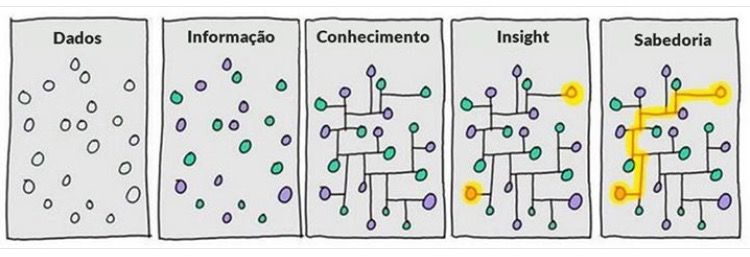
\includegraphics{dados_sabedoria.jpg}

Big Data é basicamente análise de dados. De fato isso não é nenhuma novidade. Há muitos e muitos anos a humanidade coleta dados para serem analisados. A grande inovação está em aliar métodos antigos e limitados de análise de dados aos modernos recursos de hardware de alto processamento. Ou seja, agora é possível transitar todos esses cálculos e análises por meio de softwares desenvolvidos especificamente para trabalharem com enormes quantidades de dados. Uma solução de Big Data funciona com algoritmos complexos que trabalham a informação de modo a obter como saída os mais diversos tipos de insights.

A Análise Descritiva é a fase inicial deste processo de estudo dos dados coletados. Utilizamos métodos de Estatística Descritiva para organizar, resumir e descrever os aspectos importantes de um conjunto de características observadas ou comparar tais características entre dois ou mais conjuntos. As ferramentas descritivas são os muitos tipos de gráficos e tabelas e também medidas de síntese como porcentagens, índices e médias.

Ao se condensar os dados, perde-se informação, pois não se têm as observações originais. Entretanto, esta perda de informação é pequena se comparada ao ganho que se tem com a clareza da interpretação proporcionada.

A descrição dos dados também tem como objetivo identificar anomalias, até mesmo resultante do registro incorreto de valores, e dados dispersos, aqueles que não seguem a tendência geral do restante do conjunto.

Não só nos artigos técnicos direcionados para pesquisadores, mas também nos artigos de jornais e revistas escritos para o público leigo, é cada vez mais frequente a utilização destes recursos de descrição para complementar a apresentação de um fato, justificar ou referendar um argumento.

Durante a pandemia da COVID-19 foram publicadas ótimas visualizações de dados de casos e mortes, mas a mais conhecida delas é o gráfico de John Burn-Murdoch no Financial Times. Esta é uma ótima visualização e ajudou a apresentar gráficos em escala logarítimica para um público amplo.

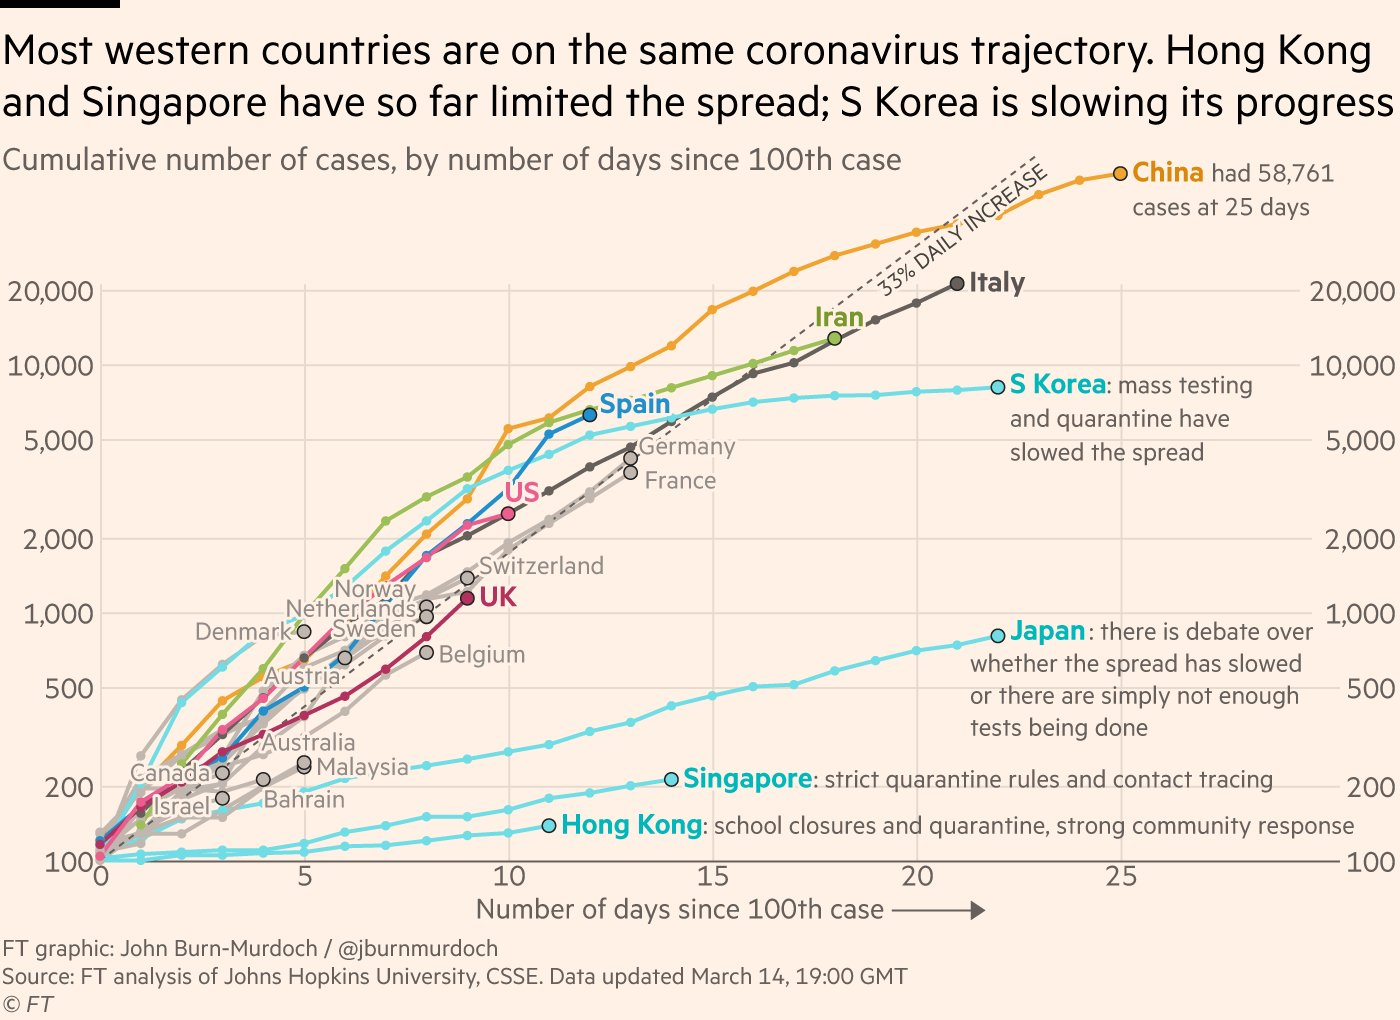
\includegraphics{financial_times.jpg}

Ao mesmo tempo em que o uso das ferramentas estatísticas vem crescendo, aumenta também o abuso de tais ferramentas. É muito comum vermos em jornais e revistas, até mesmo em periódicos científicos, gráficos - voluntariamente ou intencionalmente - enganosos e estatísticas obscuras para justificar argumentos polêmicos.

Neste capítulo iremos mergulhar no mundo da Análise de Descritiva de Dados, explorando estatísticas descritivas e análises gráficas com os pacotes mais atuais do software \(\texttt{R}\) \citep{R2020}.

\hypertarget{coleta-e-armazenamento-de-dados}{%
\section{Coleta e Armazenamento de Dados}\label{coleta-e-armazenamento-de-dados}}

\textbf{Contextualizando com um exemplo}

O primeiro caso da COVID-19 no Brasil foi confirmado em 25 de fevereiro de 2020, em São Paulo. Desde então o Governo Federal do Brasil reporta diariamente o número total de casos e mortes no país para cada Unidade da Federação, que corresponde aos 26 estados mais o Distrito Federal. No \href{https://github.com/wcota/covid19br}{github do Wesley Cota} \citep{CotaCovid19br2020} é possível extrair tais informações atualizadas para o dia anterior de forma sistematizada numa planilha de dados de maneira a realizar a entrada dos dados num programa de computador.

Para exemplificação, iremos extrair do \href{https://github.com/wcota/covid19br}{github do Wesley Cota} a planilha que possui informações agregadas para o Brasil e suas UFs. Este é o formato mais comum de uma base de dados, composta por linhas e colunas. Cada linha contém os dados de uma Unidade da Federação (elemento) e as informações (variáveis) esntão dispostas nas colunas. Dessa forma, a base de dados contém um número de linhas igual ao número de Unidades da Federação mais o total Brasil e um número de colunas igual ao número de variáveis sendo estudadas.

\begin{tabular}{l|r|r}
\hline
Estado & Casos & Mortes\\
\hline
TOTAL & 26616014 & 632946\\
\hline
AC & 105979 & 1899\\
\hline
AL & 269644 & 6478\\
\hline
AM & 549076 & 14024\\
\hline
AP & 157127 & 2059\\
\hline
BA & 1410619 & 28217\\
\hline
CE & 1183229 & 25542\\
\hline
DF & 640006 & 11230\\
\hline
ES & 934798 & 13701\\
\hline
GO & 1072457 & 25197\\
\hline
MA & 393535 & 10543\\
\hline
MG & 2880591 & 57894\\
\hline
MS & 443055 & 9992\\
\hline
MT & 656139 & 14444\\
\hline
PA & 667874 & 17458\\
\hline
PB & 521577 & 9832\\
\hline
PE & 731104 & 20736\\
\hline
PI & 352464 & 7466\\
\hline
PR & 2094041 & 41450\\
\hline
RJ & 1856969 & 70234\\
\hline
RN & 442435 & 7815\\
\hline
RO & 335746 & 6869\\
\hline
RR & 145883 & 2105\\
\hline
RS & 1932262 & 37185\\
\hline
SC & 1502015 & 20805\\
\hline
SE & 306977 & 6135\\
\hline
SP & 4749089 & 159615\\
\hline
TO & 281323 & 4021\\
\hline
\end{tabular}

Note que se usássemos uma base de dados que contém a evolução da doença por UF então teríamos uma combinação que seria uma linha para cada dia e cada estado, aumentando consideravelmente a dimensão da base.

\hypertarget{tipos-de-variuxe1veis}{%
\section{Tipos de Variáveis}\label{tipos-de-variuxe1veis}}

\textbf{Variável} é a característica de interesse que é medida em cada indivíduo da amostra ou população. Como o nome diz, seus valores variam de indivíduo para indivíduo. As variáveis podem ter valores numéricos ou não numéricos.

\hypertarget{variuxe1veis-quantitativas}{%
\section{Variáveis Quantitativas}\label{variuxe1veis-quantitativas}}

São as características que podem ser medidas em uma escala quantitativa, ou seja, apresentam valores numéricos que fazem sentido. Podem ser contínuas ou discretas.

\begin{itemize}
\tightlist
\item
  \textbf{Variáveis contínuas}: características mensuráveis que assumem valores em uma escala contínua (na reta real), para as quais valores não-inteiros (com casas decimais) fazem sentido. Usualmente devem ser medidas através de algum instrumento.

  \begin{itemize}
  \tightlist
  \item
    Exemplos: peso (balança), altura (régua), tempo (relógio), pressão arterial, idade.
  \end{itemize}
\item
  \textbf{Variáveis discretas}: características mensuráveis que podem assumir apenas um número finito ou infinito contável de valores e, assim, somente fazem sentido valores inteiros. Geralmente, são o resultado de contagens.

  \begin{itemize}
  \tightlist
  \item
    Exemplos: número de filhos, número de bactérias por litro de leite, número de casos de uma doença.
  \end{itemize}
\end{itemize}

\hypertarget{variuxe1veis-qualitativas-ou-categuxf3ricas}{%
\section{Variáveis Qualitativas (ou categóricas)}\label{variuxe1veis-qualitativas-ou-categuxf3ricas}}

São as características que não possuem valores quantitativos, mas, ao contrário, são definidas por várias categorias, ou seja, representam uma classificação dos indivíduos. Podem ser nominais ou ordinais.

\begin{itemize}
\tightlist
\item
  \textbf{Variáveis nominais}: não existe ordenação entre as categorias. Exemplos: sexo, cor dos olhos, fumante/não fumante, doente/sadio.
\item
  \textbf{Variáveis ordinais}: existe uma ordenação entre as categorias. Exemplos: escolaridade (1o, 2o, 3o graus), estágio da doença (inicial,intermediário, terminal), mês de observação (janeiro, fevereiro,\(\ldots\), dezembro).
\end{itemize}

Uma variável originalmente quantitativa pode ser coletada de forma qualitativa. Por exemplo, a variável idade, medida em anos completos, é quantitativa (contínua); mas, se for informada apenas a faixa etária (0 a 5 anos, 6 a 10 anos etc.), é qualitativa (ordinal). Outro exemplo é o peso dos lutadores de boxe, uma variável quantitativa (contínua) se trabalhamos com o valor obtido na balança, mas qualitativa (ordinal) se o classificarmos nas categorias do boxe (peso-pena, peso-leve, peso-pesado etc.).

Outro ponto importante é que nem sempre uma variável representada por números é quantitativa. O número do telefone de uma pessoa, o número da casa, o número de sua identidade. Às vezes o sexo do indivíduo é registrado na planilha de dados como 1 se macho e 2 se fêmea, por exemplo. Isto não significa que a variável sexo passou a ser quantitativa.

\hypertarget{medidas-de-tenduxeancia-central}{%
\section{Medidas de Tendência Central}\label{medidas-de-tenduxeancia-central}}

A tendência central de uma variável em um conjunto de dados é caracterizada pelo valor típico dessa variável. Essa é uma maneira de resumir a informação contida nos dados, pois escolheremos um valor para representar todos os outros. Assim, poderíamos perguntar, por exemplo, qual é a altura típica dos brasileiros adultos no final da década de 90 e compará-la com o valor típico da altura dos brasileiros no final da década de 80, a fim de verificar se os brasileiros estão se tornando, em geral, mais altos, mais baixos ou não sofreram nenhuma alteração em sua altura típica. Fazer essa comparação utilizando medidas-resumo (as alturas típicas em cada período) é bem mais sensato do que comparar os dois conjuntos de dados valor a valor, o que seria inviável. Mas, como identificar o valor típico de um conjunto de dados?

Existem três medidas que podem ser utilizadas para descrever a tendência central de um conjunto de dados: a média, a mediana e a moda. Apresentaremos essas três medidas e discutiremos suas vantagens e desvantagens.

\hypertarget{muxe9dia-aritmuxe9tica-simples}{%
\subsection{Média Aritmética Simples}\label{muxe9dia-aritmuxe9tica-simples}}

A média aritmética simples (que chamaremos apenas de média) é a medida de tendência central mais conhecida e usada para o resumo de dados. Essa popularidade pode ser devida à facilidade de cálculo e à idéia simples que ela nos sugere. De fato, se queremos um valor que represente a altura dos brasileiros adultos, por que não medir as alturas de uma amostra de brasileiros adultos, somar os valores e dividir esse ``bolo'' igualmente entre os participantes? Essa é a idéia da média aritmética.

Para apresentar a média, primeiramente vamos definir alguma notação. A princípio, essa notação pode parecer desnecessária, mas facilitará bastante nosso trabalho futuro.

\begin{equation*}
\text{Notação} 
    \begin{cases}
      n          & \text{tamanho da amostra} \\
      x_i        & \text{valor da $i$-ésima observação} \\
      \sum_{i=1}^n x & \text{soma de todas as observações} \\
      \bar x     & \text{símbolo que representa a média aritmética simples}
    \end{cases}
\end{equation*}

Assim,

\begin{equation*}
\bar x = \frac{\text{soma de todas as observações}}{{n}} = \frac{\sum_{i=1}^n x}{n}
\end{equation*}

Exemplo: No conjunto de dados (1.3, 0.7, 5.8, 2.4, 1.2), temos \(n=5\), \(x_1=\) 1.3, \(x_2=\) 0.7, \(x_3=\) 5.8, \(x_4=\) 2.4 e \(x_5=\) 1.2, portanto \(\sum_{i=1}^5 x_i=\) 1.3 + 0.7 + 5.8 + 2.4 + 1.2 \(=\) 11.4 e assim \(\bar x = \frac{11.4}{5}=2.28\).

Se esses seis valores representassem, por exemplo, as quantidades de peixe pescado (em toneladas) durante cinco dias da semana, a quantidade típica pescada por dia, naquela semana, seria 2,28 toneladas. Como estamos representando o valor típico pela média aritmética, podemos falar em quantidade média diária naquela semana.

Fazendo no \(\texttt{R}\):

\begin{Shaded}
\begin{Highlighting}[]
\FunctionTok{mean}\NormalTok{(}\FunctionTok{c}\NormalTok{(}\FloatTok{1.3}\NormalTok{, }\FloatTok{0.7}\NormalTok{, }\FloatTok{5.8}\NormalTok{, }\FloatTok{2.4}\NormalTok{, }\FloatTok{1.2}\NormalTok{))}
\end{Highlighting}
\end{Shaded}

\begin{verbatim}
## [1] 2.28
\end{verbatim}

\hypertarget{mediana}{%
\subsection{Mediana}\label{mediana}}

A mediana de um conjunto de dados é definida como sendo o ``valor do meio'' desse conjunto de dados, dispostos em ordem crescente, deixando metade dos valores acima dela e metade dos valores abaixo dela.

Como calcular a mediana? Basta seguir sua definição. Vejamos:

\begin{itemize}
\tightlist
\item
  \textbf{\(n\) é ímpar}: Existe apenas um ``valor do meio'', que é a mediana.

  \begin{itemize}
  \tightlist
  \item
    Seja o conjunto de dados (1.3, 0.7, 5.8, 2.4, 1.2).
  \item
    Ordenando os valores (0.7, 1.2, 1.3, 2.4, 5.8).
  \item
    O valor do meio é o 1.3.
  \item
    A mediana é o valor 1.3.
  \end{itemize}
\item
  \textbf{\(n\) é par}: Existem dois ``valores do meio''. A mediana é a média aritmética simples deles.

  \begin{itemize}
  \tightlist
  \item
    Seja o conjunto de dados (1.3, 0.7, 5.8, 2.4, 1.2, 2.1).
  \item
    Ordenando os valores (0.7, 1.2, 1.3, 2.1, 2.4, 5.8).
  \item
    Os valores do meio são 1.3 e 2.1.
  \item
    A mediana é (1.3+2.1)/2=1.7.
  \end{itemize}
\end{itemize}

Fazendo no \(\texttt{R}\):

\begin{Shaded}
\begin{Highlighting}[]
\FunctionTok{median}\NormalTok{(}\FunctionTok{c}\NormalTok{(}\FloatTok{1.3}\NormalTok{, }\FloatTok{0.7}\NormalTok{, }\FloatTok{5.8}\NormalTok{, }\FloatTok{2.4}\NormalTok{, }\FloatTok{1.2}\NormalTok{))}
\end{Highlighting}
\end{Shaded}

\begin{verbatim}
## [1] 1.3
\end{verbatim}

\begin{Shaded}
\begin{Highlighting}[]
\FunctionTok{median}\NormalTok{(}\FunctionTok{c}\NormalTok{(}\FloatTok{1.3}\NormalTok{, }\FloatTok{0.7}\NormalTok{, }\FloatTok{5.8}\NormalTok{, }\FloatTok{2.4}\NormalTok{, }\FloatTok{1.2}\NormalTok{, }\FloatTok{2.1}\NormalTok{))}
\end{Highlighting}
\end{Shaded}

\begin{verbatim}
## [1] 1.7
\end{verbatim}

Como medida de tendência central, a mediana é até mais intuitiva do que a média, pois representa, de fato, o centro (meio) do conjunto de valores ordenados. Assim como a média, o valor da mediana não precisa coincidir com algum dos valores do conjunto de dados. Em particular, quando os dados forem de natureza contínua, essa coincidência dificilmente ocorrerá.

\hypertarget{moda}{%
\subsection{Moda}\label{moda}}

Uma maneira alternativa de representar o que é ``típico'' é através do valor mais frequente da variável, chamado de moda.

Como calcular a moda? Basta verificar o valor que ``aparece'' mais vezes. Vejamos:

\begin{itemize}
\tightlist
\item
  No conjunto de dados (1, 2, 3, 3, 4, 5, 5, 5, 5, 5), há apenas uma moda, o valor \(5\), portanto o conjunto de dados é \textbf{unimodal}.
\item
  No conjunto de dados (1, 2, 2, 2, 2, 3, 4, 5, 6, 6, 6, 6, 7, 9), existem duas modas, os valores \(2\) e \(6\), portanto o conjunto de dados é \textbf{bimodal}.
\item
  Nem sempre a moda existe ou faz sentido, no conjunto de dados (1, 2, 3, 4, 5, 6, 7, 8, 9), não existe um valor mais frequente que os demais, portanto o conjunto de dados é \textbf{amodal}.
\end{itemize}

Para usar a função que calcula a moda (\(\texttt{Mode}\)) no \(\texttt{R}\) temos que instalar e carregar o pacote \(\texttt{pracma}\):

\begin{Shaded}
\begin{Highlighting}[]
\FunctionTok{library}\NormalTok{(pracma)}
\FunctionTok{Mode}\NormalTok{(}\FunctionTok{c}\NormalTok{(}\DecValTok{1}\NormalTok{,}\DecValTok{2}\NormalTok{,}\DecValTok{3}\NormalTok{,}\DecValTok{3}\NormalTok{,}\DecValTok{4}\NormalTok{,}\DecValTok{5}\NormalTok{,}\DecValTok{5}\NormalTok{,}\DecValTok{5}\NormalTok{,}\DecValTok{5}\NormalTok{,}\DecValTok{5}\NormalTok{))}
\end{Highlighting}
\end{Shaded}

\begin{verbatim}
## [1] 5
\end{verbatim}

\begin{Shaded}
\begin{Highlighting}[]
\FunctionTok{Mode}\NormalTok{(}\FunctionTok{c}\NormalTok{(}\DecValTok{1}\NormalTok{,}\DecValTok{2}\NormalTok{,}\DecValTok{2}\NormalTok{,}\DecValTok{2}\NormalTok{,}\DecValTok{2}\NormalTok{,}\DecValTok{3}\NormalTok{,}\DecValTok{4}\NormalTok{,}\DecValTok{5}\NormalTok{,}\DecValTok{6}\NormalTok{,}\DecValTok{6}\NormalTok{,}\DecValTok{6}\NormalTok{,}\DecValTok{6}\NormalTok{,}\DecValTok{7}\NormalTok{,}\DecValTok{9}\NormalTok{)) }\CommentTok{\# escolherá o menor valor, caso haja empate}
\end{Highlighting}
\end{Shaded}

\begin{verbatim}
## [1] 2
\end{verbatim}

\begin{Shaded}
\begin{Highlighting}[]
\FunctionTok{Mode}\NormalTok{(}\FunctionTok{c}\NormalTok{(}\DecValTok{1}\NormalTok{,}\DecValTok{2}\NormalTok{,}\DecValTok{3}\NormalTok{,}\DecValTok{4}\NormalTok{,}\DecValTok{5}\NormalTok{,}\DecValTok{6}\NormalTok{,}\DecValTok{7}\NormalTok{,}\DecValTok{8}\NormalTok{,}\DecValTok{9}\NormalTok{))}
\end{Highlighting}
\end{Shaded}

\begin{verbatim}
## [1] 1
\end{verbatim}

A moda é também a única das medidas de tendência central que faz sentido no caso de variáveis qualitativas. Assim, a categoria dessas variáveis que aparecer com maior freqüência é chamada de categoria modal.

\hypertarget{medidas-de-variabilidade}{%
\section{Medidas de Variabilidade}\label{medidas-de-variabilidade}}

As medidas de tendência central (média, mediana, moda) conseguem resumir em um único número, o valor que é ``típico'' no conjunto de dados. Mas, será que, somente com essas medidas, conseguimos descrever adequadamente o que ocorre em um conjunto de dados?

Vejamos um exemplo: quando pesamos algo em uma balança, esperamos que ela nos dê o verdadeiro peso daquilo que estamos pesando. No entanto, se fizermos várias medições do peso de um mesmo objeto em uma mesma balança, teremos diferentes valores para o peso deste objeto. Ou seja, existe variabilidade nas medições de peso fornecidas pela balança. Neste caso, quanto menor a variabilidade desses valores, mais precisa é a balança (considerando que a média das medidas de peso coincida como seu valor real). Observe na Figura abaixo, onde estão representadas as distribuições das medições do peso de uma esfera de 1000g, feitas por duas balanças (A e B). As duas balanças registram o mesmo peso médio de 1000g (média dos pesos de todas as medições feitas). Isto é, as duas balanças tipicamente acertam o verdadeiro peso da esfera. Porém, pela Figura, podemos notar que

\begin{itemize}
\tightlist
\item
  as medições da balança A \emph{variam pouco} em torno de 1000g: oscilam bastante entre cerca de 950g e 1050g (uma ``imprecisão'' de 50g)
\item
  as medições da balança B \emph{variam muito} em torno de 1000g: oscilam basicamente entre 900g e 1100g (uma ``imprecisão'' de 100g)
\end{itemize}

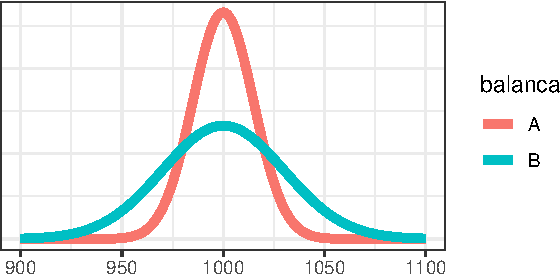
\includegraphics{inferencia_com_R_files/figure-latex/unnamed-chunk-10-1.pdf}

Dois conjuntos de dados podem ter a mesma medida de centro (valor típico), porém uma dispersão diferente em torno desse valor. Desse modo, além de uma medida que nos diga qual é o valor ``típico'' do conjunto de dados, precisamos de uma medida do grau de dispersão (variabilidade) dos dados em torno do valor típico.

O objetivo das medidas de variabilidade é quantificar esse grau de dispersão. Nesta seção, apresentaremos três dessas medidas (amplitude total, desvio-padrão e coeficiente de variação), discutindo suas vantagens e desvantagens. Em discussões posteriores, apresentaremos medidas de variabilidade alternativas.

\hypertarget{amplitude-total}{%
\subsection{Amplitude Total}\label{amplitude-total}}

A medida de variabilidade mais simples é a chamada amplitude total (AT), que é a diferença entre o valor máximo e o valor mínimo de um conjunto de dados.

\begin{equation*}
AT = \text{Máximo}-\text{Mínimo}
\end{equation*}

Exemplo: Medição do peso de uma esfera de 1000g em duas balanças (A e B).

\begin{longtable}[]{@{}lll@{}}
\toprule
Estatísticas & Balança A & Balança B \\
\midrule
\endhead
Mínimo & 945g & 895g \\
Máximo & 1040g & 1095g \\
AT & 1040-945=95g & 1095-895=200g \\
\bottomrule
\end{longtable}

A variabilidade das medições de peso da balança B é maior que a variabilidade das medições de peso da balança A (apesar do valor médio ser igual).

Embora seja uma medida simples de variabilidade, a amplitude total é um tanto grosseira, pois depende somente de dois valores do conjunto de dados (máximo e mínimo), não captando o que ocorre com os outros valores.

Fazendo no \(\texttt{R}\):

\begin{Shaded}
\begin{Highlighting}[]
\DecValTok{1040{-}945}
\end{Highlighting}
\end{Shaded}

\begin{verbatim}
## [1] 95
\end{verbatim}

\begin{Shaded}
\begin{Highlighting}[]
\DecValTok{1095{-}895}
\end{Highlighting}
\end{Shaded}

\begin{verbatim}
## [1] 200
\end{verbatim}

\hypertarget{desvio-padruxe3o}{%
\subsection{Desvio Padrão}\label{desvio-padruxe3o}}

Uma boa medida de dispersão deve considerar todos os valores do conjunto de dados e resumir o grau de dispersão desses valores em torno do valor típico.

Considerando a média como a medida de tendência central, podemos pensar em medir a dispersão (desvio) de cada valor do conjunto de dados em relação à ela. A medida mais simples de desvio entre duas quantidades é a diferença entre elas. Assim, para cada valor \(x_i\), teremos o seu desvio em relação à \(\bar x\) representado por \((x_i-\bar x)\).

Exemplo: No conjunto de dados 1, 1, 2, 3, 4, 4, 5, 6, 7, 7, relativo ao número de filhos de 10 mulheres, temos \(\bar x = 4\) filhos. Na tabela abaixo, a coluna 1 mostra esses 10 valores e a coluna 2 mostra o desvio de cada um deles até a média.

\begin{tabular}{l|l|l}
\hline
Coluna 1 (Xi) & Coluna 2 (Xi-Media) & Coluna 3 (Xi-Media)\textasciicircum{}2\\
\hline
1 & -3 & 9\\
\hline
1 & -3 & 9\\
\hline
2 & -2 & 4\\
\hline
3 & -1 & 1\\
\hline
4 & 0 & 0\\
\hline
4 & 0 & 0\\
\hline
5 & 1 & 1\\
\hline
6 & 2 & 4\\
\hline
7 & 3 & 9\\
\hline
7 & 3 & 9\\
\hline
Soma & 0 & 46\\
\hline
\end{tabular}

\textbf{A ideia do desvio padrão}

Como temos um desvio para cada elemento, poderíamos pensar em resumi-los em um desvio típico, a exemplo do que fizemos com a média. Porém, quando somarmos esses desvios para o cálculo do desvio médio, a soma dará sempre zero, como pode ser visto na coluna 2 do exemplo anterior. Isto ocorre com qualquer conjunto de dados, pois os desvios negativos sempre compensaram os positivos.

No entanto, os sinais dos desvios não são importantes para nossa medida de dispersão, já que estamos interessados na quantidade de dispersão e não na direção dela. Portanto, eliminaremos os sinais elevando os desvios ao quadrado, como mostrado na coluna 3. A soma desses desvios ao quadrado pode ser, então, dividida entre os participantes do ``bolo''. Na verdade, por razões absolutamente teóricas, dividiremos essa soma pelo total de participantes menos 1 \((n-1)\). Assim, usando a notação definida anteriormente, teremos

\begin{equation*}
\frac{\sum_{i=1}^n (x_i-\bar x)^2}{n-1}
\end{equation*}

Para os dados do exemplo, teremos \(46/(10-1)=5,11\). Esse valor pode ser visto como uma quase-média dos desvios ao quadrado e é chamado de \textbf{variância}.

A variância seria nossa medida de variabilidade se não fosse o fato de que ela está expressa em uma unidade diferente da unidade dos dados, pois, ao elevarmos os desvios ao quadrado, elevamos também as unidades de medida em que eles estão expressos. No caso dos dados do exemplo, medidos em número de filhos, a variância vale \(5,11\) ``filhos ao quadrado'', algo que não faz nenhum sentido.

Para eliminar esse problema, extraímos a raiz quadrada da variância e, finalmente, temos a nossa medida de variabilidade, que chamaremos desvio-padrão (DP).

\begin{equation*}
DP=\sqrt{\frac{\sum_{i=1}^n (x_i-\bar x)^2}{n-1}}
\end{equation*}

O desvio-padrão, como o nome já diz, representa o desvio típico dos dados em relação à média, escolhida como medida de tendência central. No exemplo, temos que o desvio padrão vale \(2,26\). Isto significa que a distância típica (padrão) de cada mãe até o número médio de filhos (4 filhos) é de 2,26 filhos. Quanto maior o desvio-padrão, mais diferentes entre si serão as quantidades de filhos de cada mãe.

O desvio-padrão, em alguns livros chamado de \(s\), é uma medida sempre positiva. Se observarmos a maneira como ele é calculado, veremos que não há como obter um valor
negativo.

Fazendo no \(\texttt{R}\):

\begin{Shaded}
\begin{Highlighting}[]
\FunctionTok{round}\NormalTok{(}\FunctionTok{var}\NormalTok{(}\FunctionTok{c}\NormalTok{(}\DecValTok{1}\NormalTok{,}\DecValTok{1}\NormalTok{,}\DecValTok{2}\NormalTok{,}\DecValTok{3}\NormalTok{,}\DecValTok{4}\NormalTok{,}\DecValTok{4}\NormalTok{,}\DecValTok{5}\NormalTok{,}\DecValTok{6}\NormalTok{,}\DecValTok{7}\NormalTok{,}\DecValTok{7}\NormalTok{)),}\DecValTok{2}\NormalTok{) }\CommentTok{\# função round() serve para arrendondar o número de dígitos}
\end{Highlighting}
\end{Shaded}

\begin{verbatim}
## [1] 5.11
\end{verbatim}

\begin{Shaded}
\begin{Highlighting}[]
\FunctionTok{round}\NormalTok{(}\FunctionTok{sd}\NormalTok{(}\FunctionTok{c}\NormalTok{(}\DecValTok{1}\NormalTok{,}\DecValTok{1}\NormalTok{,}\DecValTok{2}\NormalTok{,}\DecValTok{3}\NormalTok{,}\DecValTok{4}\NormalTok{,}\DecValTok{4}\NormalTok{,}\DecValTok{5}\NormalTok{,}\DecValTok{6}\NormalTok{,}\DecValTok{7}\NormalTok{,}\DecValTok{7}\NormalTok{)),}\DecValTok{2}\NormalTok{)}
\end{Highlighting}
\end{Shaded}

\begin{verbatim}
## [1] 2.26
\end{verbatim}

Exemplo: Os agentes de fiscalização de certo município realizam, periodicamente, uma vistoria nos bares e restaurantes para apurar possíveis irregularidades na venda de seus produtos. A seguir, são apresentados dados de uma vistoria sobre os pesos (em gramas) de uma amostra de 10 bifes, constantes de um cardápio de um restaurante como ``bife de 200 gramas''.

\begin{verbatim}
##  [1] 170 175 180 185 190 195 200 200 200 205
\end{verbatim}

Como podemos notar, nem todos os ``bifes de 200 gramas'' pesam realmente 200 gramas. Esta variação é natural e é devida ao processo de produção dos bifes. No entanto, esses bifes deveriam pesar cerca de 200 gramas e com pouca variação em torno desse valor. Com o auxílio do \(\texttt{R}\), calcularemos a média e o desvio-padrão.

\begin{Shaded}
\begin{Highlighting}[]
\FunctionTok{mean}\NormalTok{(}\FunctionTok{c}\NormalTok{(}\DecValTok{170}\NormalTok{,}\DecValTok{175}\NormalTok{,}\DecValTok{180}\NormalTok{,}\DecValTok{185}\NormalTok{,}\DecValTok{190}\NormalTok{,}\DecValTok{195}\NormalTok{,}\DecValTok{200}\NormalTok{,}\DecValTok{200}\NormalTok{,}\DecValTok{200}\NormalTok{,}\DecValTok{205}\NormalTok{))}
\end{Highlighting}
\end{Shaded}

\begin{verbatim}
## [1] 190
\end{verbatim}

\begin{Shaded}
\begin{Highlighting}[]
\FunctionTok{sd}\NormalTok{(}\FunctionTok{c}\NormalTok{(}\DecValTok{170}\NormalTok{,}\DecValTok{175}\NormalTok{,}\DecValTok{180}\NormalTok{,}\DecValTok{185}\NormalTok{,}\DecValTok{190}\NormalTok{,}\DecValTok{195}\NormalTok{,}\DecValTok{200}\NormalTok{,}\DecValTok{200}\NormalTok{,}\DecValTok{200}\NormalTok{,}\DecValTok{205}\NormalTok{))}
\end{Highlighting}
\end{Shaded}

\begin{verbatim}
## [1] 12.0185
\end{verbatim}

Os bifes desse restaurante pesam, em média, 190 gramas, com um desvio-padrão de 12 gramas. Ou seja, os pesos dos ``bifes de 200 gramas'' variam tipicamente entre 178 e 202 gramas. Analisando esses valores, concluímos que esse restaurante pode estar lesando a maior parte de seus clientes.

Para casos como esse, os agentes fiscalizadores podem estabelecer parâmetros (valores) para saber até quanto a média pode se desviar do valor correto e o quanto de variação eles podem permitir numa amostra para concluir que o processo de produção de bifes não possui problemas. Por exemplo, a média da amostra não poderia ser inferior a 198 gramas, com um desvio-padrão que não seja superior a 5\% dessa média.

Essas idéias são utilizadas no controle do processo de produção das indústrias, onde já se espera alguma variação entre as unidades produzidas. Porém, essa variação deve estar sob controle. Numa indústria farmacêutica, por exemplo, espera-se que os comprimidos de uma certa droga sejam produzidos com uma certa variação em sua composição (maior ou menor quantidade do princípio ativo), devido à própria maneira como os comprimidos são produzidos (máquinas, pessoas etc.). No entanto, esta variação deve ser pequena, para que não sejam produzidos comprimidos inócuos (com pouco do princípio ativo) ou com extra-dosagem do princípio ativo, o que, em ambos os casos, pode causar sérias complicações à saúde do paciente.

O desvio-padrão nos permite distinguir numericamente conjuntos de dados de mesmo tamanho, mesma média, mas que são visivelmente diferentes. Usando o desvio-padrão, também conseguimos representar numericamente a variabilidade das medições das balanças A e B, que, apesar de possuírem a mesma média, possuem variabilidades bastante diferentes.

Quando os conjuntos de dados a serem comparados possuem médias diferentes, a comparação da variabilidade desses conjuntos deve levar em conta essa diferença. Por esta e outras razões, definiremos uma terceira medida de variabilidade, o \textbf{coeficiente de variação}.

\hypertarget{coeficiente-de-variauxe7uxe3o}{%
\subsection{Coeficiente de Variação}\label{coeficiente-de-variauxe7uxe3o}}

Ao analisarmos o grau de dispersão de um conjunto de dados, poderemos nos deparar com uma questão do tipo: um desvio-padrão de 10 unidades é pequeno ou grande?

Vejamos:

\begin{itemize}
\tightlist
\item
  Se estivermos trabalhando com um conjunto de dados cuja média é 10.000, um desvio típico de 10 unidades em torno dessa média significa pouca dispersão;
\item
  Mas, se a média for igual a 100, um desvio típico de 10 unidades em torno dessa média significa muita dispersão.
\end{itemize}

Assim, antes de responder se um desvio-padrão de 10 unidades é grande ou pequeno, devemos avaliar sua magnitude em relação à média:

\begin{itemize}
\tightlist
\item
  No primeiro caso, o desvio-padrão corresponde a 0,1\% da média
\item
  No segundo caso, o desvio-padrão corresponde a 10\% da média
\end{itemize}

À essa razão entre o desvio-padrão e a média damos o nome de \textbf{Coeficiente de Variação}:

\begin{equation*}
CV=\frac{\text{Desvio Padrão}}{\text{Média}}
\end{equation*}

Quanto menor o Coeficiente de Variação de um conjunto de dados, menor é a sua variabilidade. O Coeficiente de Variação expressa o quanto da escala de medida, representada pela média, é ocupada pelo desvio-padrão.

O Coeficiente de Variação é uma medida adimensional, isto é, não depende da unidade de medida. Essa característica nos permite usá-lo para comparar a variabilidade de conjuntos de dados medidos em unidades diferentes, o que seria impossível usando o desvio-padrão.

Exemplo: Numa pesquisa na área de Saúde Ocupacional, deseja-se comparar a idade de motoristas e cobradores de ônibus da região metropolitana de Belo Horizonte. Algumas estatísticas descritivas são apresentadas na Tabela abaixo.

\begin{tabular}{l|r|r|r|r}
\hline
Grupo & n & Media & DP & CV\\
\hline
Motoristas & 150 & 35.6 & 5.08 & 0.143\\
\hline
Cobradores & 50 & 22.6 & 3.11 & 0.137\\
\hline
\end{tabular}

Os motoristas são, em média, 13 anos mais velhos do que os cobradores. Ao compararmos o grau de dispersão dos dois grupos usando o desvio-padrão, concluiríamos que os motoristas são menos homogêneos quanto à idade do que os cobradores. Ao fazermos isso, estamos esquecendo que, apesar de estarem em unidades iguais, as medidas de idade nos dois grupos variam em escalas diferentes. As idades dos motoristas variam em torno dos 35 anos e podem chegar até 18 anos (idade mínima para se conseguir a habilitação), numa amplitude de 17 unidades. Enquanto isso, as idades dos cobradores variam em torno de 22 anos e também só podem chegar até a 18 anos, uma amplitude de apenas 4 anos. Assim, os motoristas tem a possibilidade de ter um desvio-padrão maior do que o dos cobradores. Se levarmos em conta a escala de medida, usando o coeficiente de variação, veremos que os motoristas são somente um pouco mais heterogêneos (dispersos) quanto à idade do que os cobradores.

Fazendo no \(\texttt{R}\):

\begin{Shaded}
\begin{Highlighting}[]
\NormalTok{media}\OtherTok{=}\FunctionTok{c}\NormalTok{(}\FloatTok{35.6}\NormalTok{,}\FloatTok{22.6}\NormalTok{)}
\NormalTok{desvio}\OtherTok{=}\FunctionTok{c}\NormalTok{(}\FloatTok{5.08}\NormalTok{,}\FloatTok{3.11}\NormalTok{)}
\FunctionTok{round}\NormalTok{(desvio}\SpecialCharTok{/}\NormalTok{media,}\DecValTok{3}\NormalTok{)}
\end{Highlighting}
\end{Shaded}

\begin{verbatim}
## [1] 0.143 0.138
\end{verbatim}

\hypertarget{medidas-de-posiuxe7uxe3o}{%
\section{Medidas de Posição}\label{medidas-de-posiuxe7uxe3o}}

Quando falamos de posição ou colocação de um indivíduo em uma corrida ou em um teste como o Vestibular, frequentemente nos referimos ao seu posto, como 1º, 2º, 3º, 29º ou último lugar. Mas, para sabermos se uma dada colocação é ou não um bom resultado, precisamos informar quantos indivíduos participaram da corrida ou do Vestibular.

A medida de posição que veremos aqui, os percentis, solucionam este e outros problemas de posicionamento (ranking). A posição de um indivíduo no conjunto de dados é mostrada, pelo percentil, contando-se (em porcentagem) quantos indivíduos do conjunto têm valores menores que o deste indivíduo.

Como veremos, esta medida de posição pode ser usada para comparar a posição do indivíduo em diferentes conjuntos de dados, nos quais foram medidas as mesmas variáveis ou variáveis diferentes.

\hypertarget{percentis}{%
\subsection{Percentis}\label{percentis}}

Considere o trecho a seguir, sobre a posição do Brasil, entre os países do mundo, quanto à renda per capita:

\emph{O Brasil obviamente não é país rico, mas também não está entre os mais pobres. \(\ldots\) Mais de três quartos da população mundial vivem em países de renda per capita menor}

Neste caso, o posição do Brasil é dada pela quantidade de países que têm renda per capita menores que o Brasil, a saber três quartos ou \(75\%\). O mesmo tipo de raciocínio fazemos quando dizemos que certo aluno está entre os \(5\%\) melhores do colégio. Não precisamos nem saber quantos alunos tem o colégio ou em quantos países estão sendo consideradas as rendas. Aqui já houve uma padronização da posição usando-se a porcentagem de alunos ou países com desempenho ou renda abaixo do valor considerado. É este raciocínio que define os percentis.

\textbf{O percentil de ordem $K$ (onde $k$ é qualquer valor entre $0$ e $100$), denotado por $P_k$, é o valor tal que $K\%$ dos valores do conjunto de dados são menores ou iguais a ele.}

Assim, o percentil de ordem \(10\), o \(P_{10}\), é o valor da variável tal que \(10\%\) dos valores são menores ou iguais a ele; o percentil de ordem \(65\) deixa \(65\%\) dos dados menores ou iguais a ele etc.

Os percentil de ordem \(10,20,30,\ldots,90\) dividem o conjunto de dados em dez partes com mesmo número de observações e são chamados de \textbf{decis}.

Os percentis de ordem \(25,50\) e \(75\) dividem o conjunto de dados em quatro partes com o mesmo número de observações. Assim, estes três percentis recebem o nome de quartis -- \textbf{primeiro quartil (Q1), segundo quartil (Q2) e terceiro quartil (Q3)}, respectivamente. O segundo quartil é a já conhecida mediana.

Existem vários processos para calcular os percentis, usando interpolação. Vamos ficar com um método mais simples, mostrado na Figura a seguir. As diferenças serão muito pequenas e desaparecerão à medida que aumenta o número de dados.

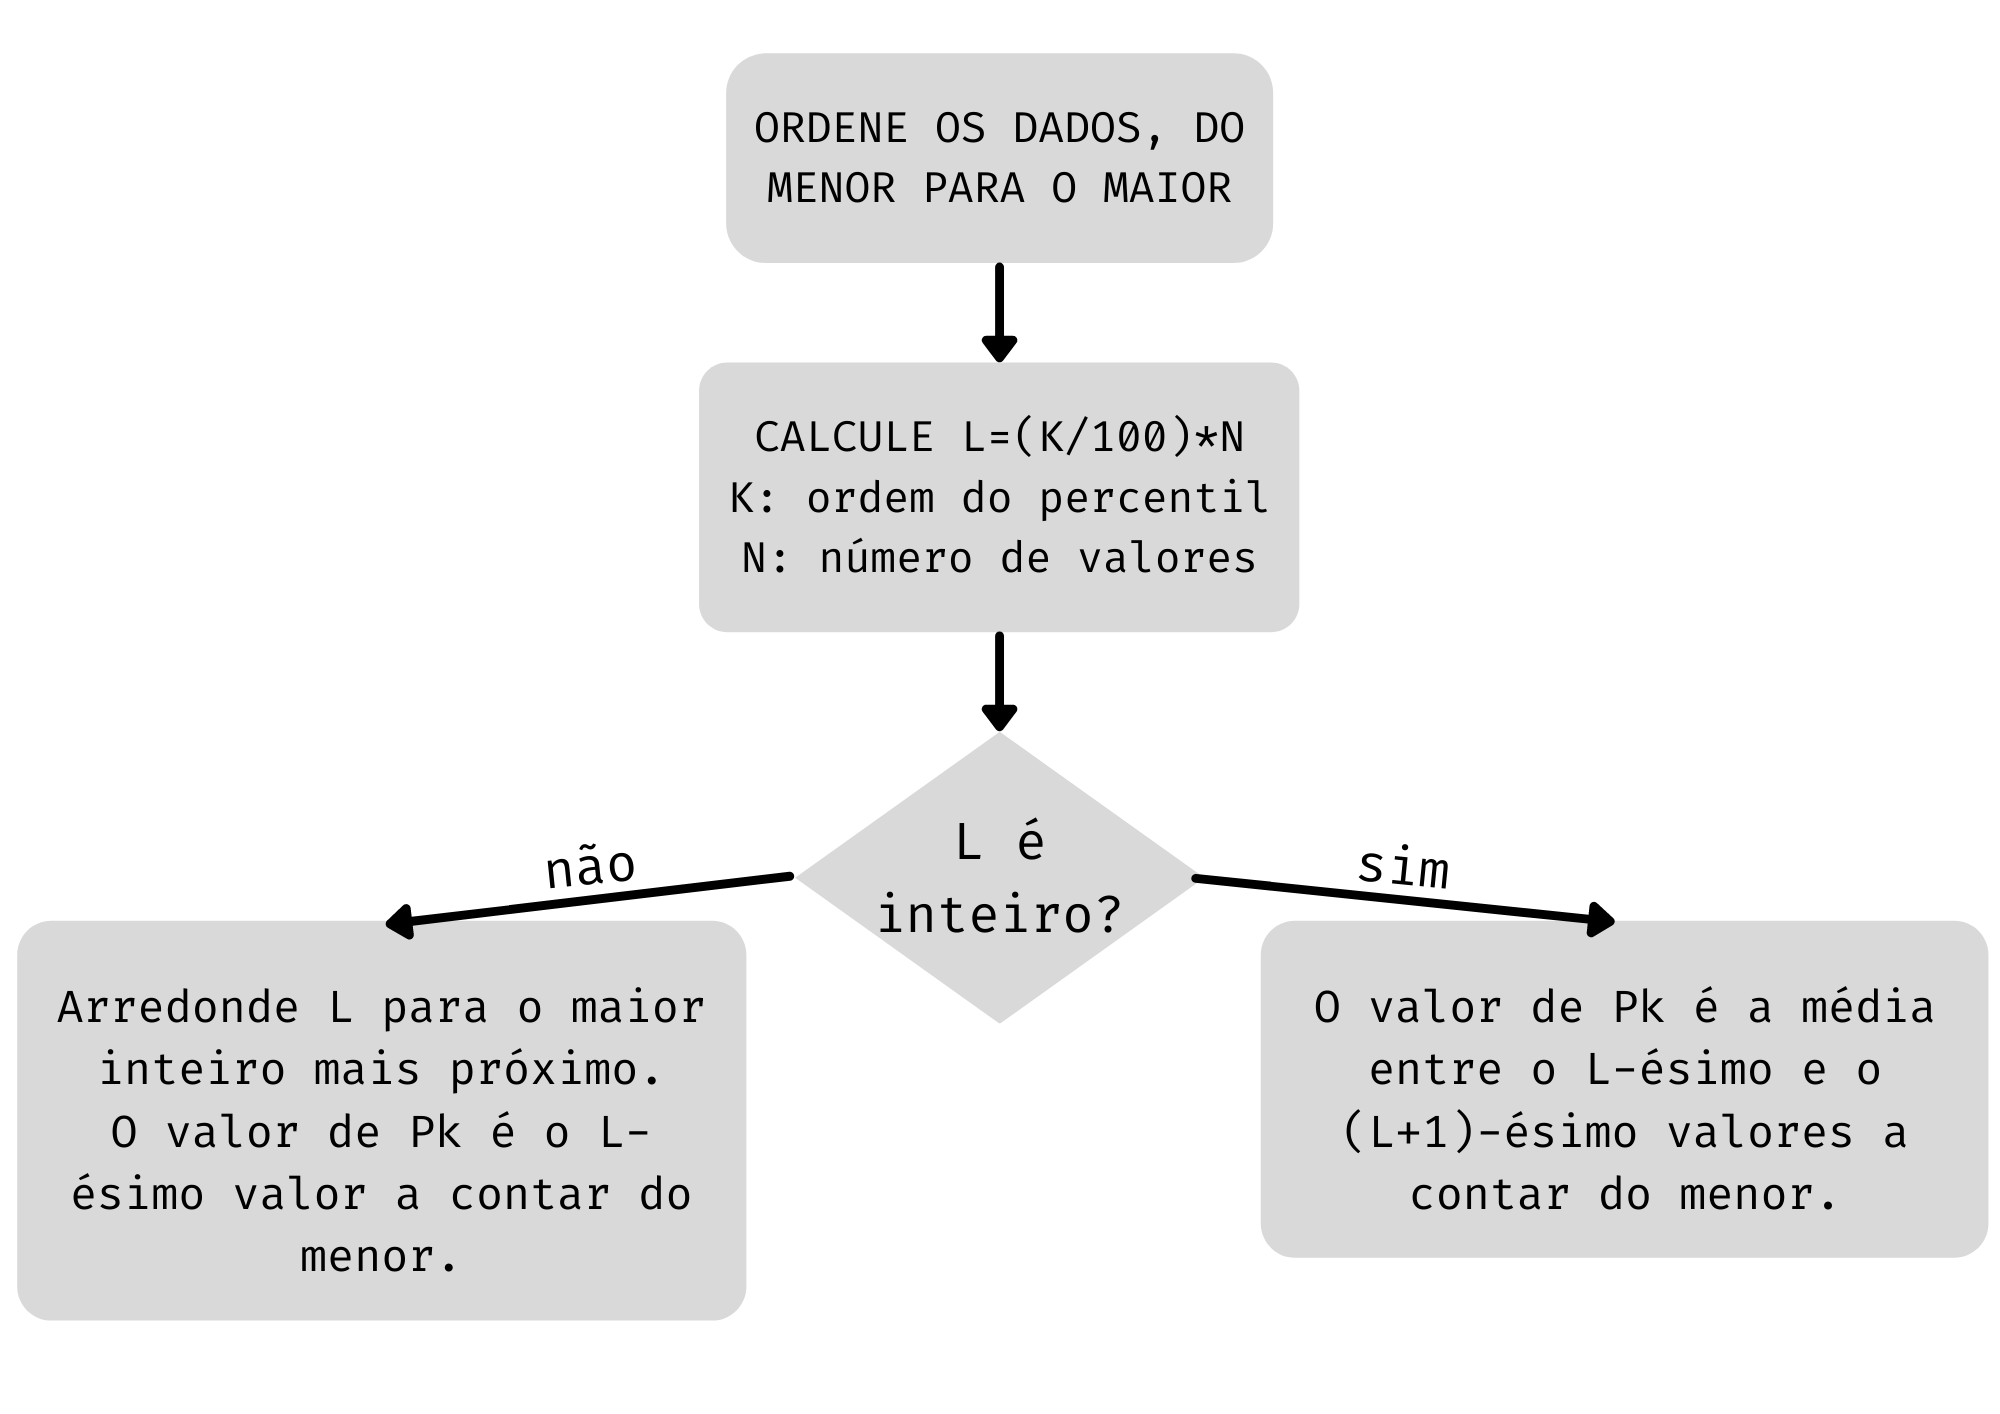
\includegraphics{fluxograma_percentil.png}

Considere as notas finais dos 40 candidatos ao curso de Direito no Vestibular de certa faculdade, já colocadas em ordem crescente:

\begin{verbatim}
##  [1] 40 41 42 42 44 47 48 48 49 49 51 52 53 58 59 62 63 64 65 66 67 68 69 70 75
## [26] 76 83 83 85 86 86 87 87 88 92 93 94 95 97 98
\end{verbatim}

Vamos calcular alguns percentis:

\begin{itemize}
\item
  Percentil de ordem \(10\): \(10\%\) de \(40=4\). Então o \(P_10\) = média(4º e 5º valores)=\((42+44)/2=43\).
\item
  Percentil de ordem \(95\): \(95\%\) de \(40=38\). Então o \(P_95\) = média(38º e 39º valores)=\((95+97)/2=96\).
\item
  Primeiro Quartil: \(25\%\) de \(40=10\). Então o Q1 = média(10º e 11º valores)=\((49+51)/2 = 50\).
\item
  Terceiro Quartil: \(75\%\) de \(40=30\). Então o Q3 = média(30º e 31º valores)=\((86+86)/2 = 86\).
\item
  Mediana: \(50\%\) de \(40=20\). Então mediana = média(20º e 21º valores)=\((66+67)/2 = 66,5\).
\end{itemize}

Fazendo no \(\texttt{R}\):

\begin{Shaded}
\begin{Highlighting}[]
\NormalTok{dados\_ex7}\OtherTok{=}\FunctionTok{c}\NormalTok{(}\DecValTok{40}\NormalTok{,}\DecValTok{41}\NormalTok{,}\DecValTok{42}\NormalTok{,}\DecValTok{42}\NormalTok{,}\DecValTok{44}\NormalTok{,}\DecValTok{47}\NormalTok{,}\DecValTok{48}\NormalTok{,}\DecValTok{48}\NormalTok{,}\DecValTok{49}\NormalTok{,}
            \DecValTok{49}\NormalTok{,}\DecValTok{51}\NormalTok{,}\DecValTok{52}\NormalTok{,}\DecValTok{53}\NormalTok{,}\DecValTok{58}\NormalTok{,}\DecValTok{59}\NormalTok{,}\DecValTok{62}\NormalTok{,}\DecValTok{63}\NormalTok{,}\DecValTok{64}\NormalTok{,}
            \DecValTok{65}\NormalTok{,}\DecValTok{66}\NormalTok{,}\DecValTok{67}\NormalTok{,}\DecValTok{68}\NormalTok{,}\DecValTok{69}\NormalTok{,}\DecValTok{70}\NormalTok{,}\DecValTok{75}\NormalTok{,}\DecValTok{76}\NormalTok{,}\DecValTok{83}\NormalTok{,}
            \DecValTok{83}\NormalTok{,}\DecValTok{85}\NormalTok{,}\DecValTok{86}\NormalTok{,}\DecValTok{86}\NormalTok{,}\DecValTok{87}\NormalTok{,}\DecValTok{87}\NormalTok{,}\DecValTok{88}\NormalTok{,}\DecValTok{92}\NormalTok{,}\DecValTok{93}\NormalTok{,}\DecValTok{94}\NormalTok{,}\DecValTok{95}\NormalTok{,}\DecValTok{97}\NormalTok{,}\DecValTok{98}\NormalTok{)}
\FunctionTok{quantile}\NormalTok{(dados,}\AttributeTok{probs=}\FunctionTok{c}\NormalTok{(}\FloatTok{0.1}\NormalTok{,}\FloatTok{0.95}\NormalTok{,}\FloatTok{0.25}\NormalTok{,}\FloatTok{0.75}\NormalTok{,}\FloatTok{0.5}\NormalTok{))}
\end{Highlighting}
\end{Shaded}

\begin{verbatim}
##    10%    95%    25%    75%    50% 
## 174.50 202.75 181.25 200.00 192.50
\end{verbatim}

Veja que os valores encontrados pelo \(\texttt{R}\) não coincidem com os calculados ``na mão'', isto porque, o \(\texttt{R}\) utiliza um método de interpolação para calcular valores que não estão presentes na amostra.

\hypertarget{referuxeancias}{%
\section{Referências}\label{referuxeancias}}

\hypertarget{anuxe1lise-gruxe1fica}{%
\chapter{Análise Gráfica}\label{anuxe1lise-gruxe1fica}}

Já sabemos que as variáveis de um estudo dividem-se em quatro tipos:

\begin{itemize}
\tightlist
\item
  \textbf{Qualitativas}:

  \begin{itemize}
  \tightlist
  \item
    nominais
  \item
    ordinais
  \end{itemize}
\item
  \textbf{Quantitativas}:

  \begin{itemize}
  \tightlist
  \item
    discretas
  \item
    contínuas
  \end{itemize}
\end{itemize}

Os dados gerados por esses tipos de variáveis são de naturezas diferentes e devem receber tratamentos diferentes. Portanto, vamos estudar as ferramentas mais adequadas para cada tipo de dados, separadamente.

\hypertarget{variuxe1veis-qualitativas---nominais-e-ordinais}{%
\section{Variáveis Qualitativas - Nominais e Ordinais}\label{variuxe1veis-qualitativas---nominais-e-ordinais}}

Na base de dados \(\texttt{mtcars}\), uma das duas variáveis qualitativas presentes é a categoria da transmissão (automática ou manual). Para organizar os dados provenientes de uma variável qualitativa, é usual fazer uma tabela de frequências, como a tabela abaixo, onde estão apresentadas as frequências com que ocorre cada um dos tipos de transmissão no total dos 32 carros observados. Cada categoria da variável transmissão (automática, manual) é representada numa linha da tabela. Há uma coluna com as contagens de carros em cada categoria (frequência absoluta) e outra com os percentuais que essas contagens representam no total de carros (frequência relativa). Esse tipo de tabela representa a distribuição de frequências dos carros segundo a variável transmissão.

Como a variável transmissão é qualitativa nominal, ou seja, não há uma ordem natural em suas categorias, a ordem das linhas da tabela pode ser qualquer uma. É comum a disposição das linhas pela ordem decrescente das frequências das classes.

\begin{tabular}{l>{\raggedleft\arraybackslash}p{2.5cm}>{\raggedleft\arraybackslash}p{2.5cm}}
\toprule
Transmissão & Frequência Absoluta & Frequência Relativa (\%)\\
\midrule
Automático & 19 & 59.38\\
Manual & 13 & 40.62\\
Total & 32 & 100.00\\
\bottomrule
\end{tabular}

Quando a variável tabelada for do tipo qualitativa ordinal, as linhas da tabela de frequências devem ser dispostas na ordem existente para as categorias. A tabela abaixo mostra a distribuição de
frequências das coletas segundo o mês de observação na base de dados \(\texttt{airquality}\), que é uma variável qualitativa ordinal. Nesse caso, podemos acrescentar mais duas colunas com as frequências acumuladas (absoluta e relativa), que mostram, para cada mês, a frequência das coletas até aquele mês. Por exemplo, até o mês de julho, foram coletadas 92 amostras, o que representa 60,13\% do total de amostras coletadas.

\begin{tabular}{l>{\raggedleft\arraybackslash}p{2.5cm}>{\raggedleft\arraybackslash}p{2.5cm}>{\raggedright\arraybackslash}p{2.5cm}>{\raggedright\arraybackslash}p{2.5cm}}
\toprule
Transmissão & Frequência Absoluta & Frequência Relativa (\%) & Frequência Absoluta Acumulada & Frequência Relativa Acumulada (\%)\\
\midrule
5 & 31 & 20.26 & 31 & 20.26\\
6 & 30 & 19.61 & 61 & 39.87\\
7 & 31 & 20.26 & 92 & 60.13\\
8 & 31 & 20.26 & 123 & 80.39\\
9 & 30 & 19.61 & 153 & 100\\
\addlinespace
Total & 153 & 100.00 & - & -\\
\bottomrule
\end{tabular}

Note que as frequências acumuladas não fazem sentido em distribuição de frequências de variáveis para as quais não existe uma ordem natural nas categorias, as qualitativas nominais.

A visualização da distribuição de frequências de uma variável fica mais fácil se fizermos um gráfico a partir da tabela de frequências. Existem vários tipos de gráficos, dependendo do tipo de variável a ser representada. Para as variáveis do tipo qualitativas, abordaremos dois tipos de gráficos: os de setores e os de barras.

Os gráficos de setores, mais conhecidos como gráficos de pizza ou torta, são construídos dividindo-se um círculo (pizza) em setores (fatias), um para cada categoria, que serão proporcionais à frequência daquela categoria.

A Figura a seguir mostra um gráfico de setores para a variável transmissão, construído a partir da primeira tabela de frequências. Através desse gráfico, fica mais fácil perceber que os carros automáticos são a grande maioria dos carros. Como esse gráfico contém todas as informações da tabela, pode substituí-la com a vantagem de tornar análise dessa variável mais agradável.

\begin{Shaded}
\begin{Highlighting}[]
\FunctionTok{library}\NormalTok{(ggplot2)}
\NormalTok{df }\OtherTok{=} \FunctionTok{data.frame}\NormalTok{(}\FunctionTok{table}\NormalTok{(mtcars}\SpecialCharTok{$}\NormalTok{am))}
\FunctionTok{levels}\NormalTok{(df}\SpecialCharTok{$}\NormalTok{Var1) }\OtherTok{=} \FunctionTok{c}\NormalTok{(}\StringTok{"Automático"}\NormalTok{,}\StringTok{"Manual"}\NormalTok{)}
\FunctionTok{ggplot}\NormalTok{(df, }\FunctionTok{aes}\NormalTok{(}\AttributeTok{x=}\StringTok{""}\NormalTok{, }\AttributeTok{y=}\NormalTok{Freq, }\AttributeTok{fill=}\NormalTok{Var1)) }\SpecialCharTok{+}
  \FunctionTok{geom\_bar}\NormalTok{(}\AttributeTok{stat=}\StringTok{"identity"}\NormalTok{) }\SpecialCharTok{+}
  \FunctionTok{coord\_polar}\NormalTok{(}\StringTok{"y"}\NormalTok{, }\AttributeTok{start=}\DecValTok{0}\NormalTok{) }\SpecialCharTok{+}
  \FunctionTok{theme\_void}\NormalTok{() }\SpecialCharTok{+}
  \FunctionTok{theme}\NormalTok{(}\AttributeTok{legend.title =} \FunctionTok{element\_blank}\NormalTok{())}
\end{Highlighting}
\end{Shaded}

\begin{center}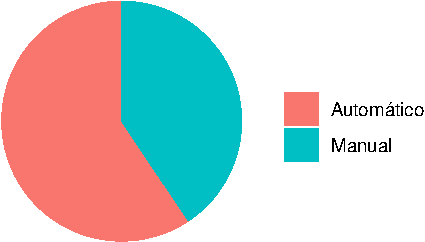
\includegraphics{inferencia_com_R_files/figure-latex/unnamed-chunk-24-1} \end{center}

Quando houver mais de duas categorias de uma variável nominal, a disposição no gráfico de setores deve ser pela ordem decrescente das frequências, no sentido horário. A categoria ``outros'', quando existir, deve ser sempre a última, mesmo não seja a de menor frequência.

As vantagens da representação gráfica das distribuições de frequências ficam ainda mais evidentes quando há a necessidade de comparar vários grupos com relação à variáveis que possuem muitas categorias, como veremos mais adiante.

Uma alternativa ao gráfico de setores é o gráfico de barras (colunas) como o da figura a seguir. Ao invés de dividirmos um círculo, dividimos uma barra. Note que, em ambos os gráficos, as frequências relativas das categorias devem somar 100\%. Aliás, esse é a idéia dos gráficos: mostrar como se dá a divisão (distribuição) do total de elementos (100\%) em partes (fatias).

\begin{Shaded}
\begin{Highlighting}[]
\NormalTok{df }\OtherTok{=} \FunctionTok{data.frame}\NormalTok{(}\FunctionTok{table}\NormalTok{(mtcars}\SpecialCharTok{$}\NormalTok{am))}
\FunctionTok{levels}\NormalTok{(df}\SpecialCharTok{$}\NormalTok{Var1) }\OtherTok{=} \FunctionTok{c}\NormalTok{(}\StringTok{"Automático"}\NormalTok{,}\StringTok{"Manual"}\NormalTok{)}
\FunctionTok{ggplot}\NormalTok{(df, }\FunctionTok{aes}\NormalTok{(}\AttributeTok{x=}\NormalTok{Var1, }\AttributeTok{y=}\NormalTok{Freq, }\AttributeTok{fill=}\NormalTok{Var1)) }\SpecialCharTok{+}
  \FunctionTok{geom\_bar}\NormalTok{(}\AttributeTok{stat=}\StringTok{"identity"}\NormalTok{) }\SpecialCharTok{+}
  \FunctionTok{geom\_text}\NormalTok{(}\FunctionTok{aes}\NormalTok{(}\AttributeTok{label =}\NormalTok{ Freq),}\AttributeTok{position=}\FunctionTok{position\_stack}\NormalTok{(}\AttributeTok{vjust =} \FloatTok{0.5}\NormalTok{)) }\SpecialCharTok{+}
  \FunctionTok{theme}\NormalTok{(}\AttributeTok{legend.title =} \FunctionTok{element\_blank}\NormalTok{(),}
        \AttributeTok{axis.title.x =} \FunctionTok{element\_blank}\NormalTok{(),}
        \AttributeTok{axis.ticks.x =} \FunctionTok{element\_blank}\NormalTok{(),}
        \AttributeTok{axis.title.y =} \FunctionTok{element\_blank}\NormalTok{())}
\end{Highlighting}
\end{Shaded}

\begin{center}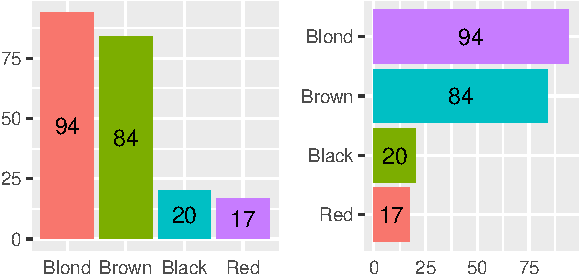
\includegraphics{inferencia_com_R_files/figure-latex/unnamed-chunk-25-1} \end{center}

Uma situação diferente ocorre quando desejamos comparar a distribuição de frequências de uma mesma variável em vários grupos, como por exemplo, a frequência de estudantes com olhos azuis entre todas as cores de cabelo na base de dados \(\texttt{HairEyeColor}\). Se quisermos usar o gráfico de setores para fazer essa comparação, devemos fazer quatro gráficos, um para cada cor de cabelo, com duas fatias cada um (olhos azuis e olhos não azuis). Uma alternativa é a construção de um gráfico de colunas (barras) como os gráficos das figuras a seguir, onde há uma barra para cada cor de cabelo representando a frequência de estudantes com olhos azuis e aquela cor de cabelo. Além de economizar espaço na apresentação, permite que as comparações sejam feitas de maneira mais rápida.

\begin{Shaded}
\begin{Highlighting}[]
\NormalTok{df }\OtherTok{=} \FunctionTok{data.frame}\NormalTok{(HairEyeColor[,,}\DecValTok{1}\NormalTok{] }\SpecialCharTok{+}\NormalTok{ HairEyeColor[,,}\DecValTok{2}\NormalTok{])}
\NormalTok{df }\OtherTok{=}\NormalTok{ df }\SpecialCharTok{\%\textgreater{}\%} \FunctionTok{filter}\NormalTok{(Eye }\SpecialCharTok{==} \StringTok{"Blue"}\NormalTok{)}
\NormalTok{p1 }\OtherTok{=}\NormalTok{ df }\SpecialCharTok{\%\textgreater{}\%} \FunctionTok{mutate}\NormalTok{(}\AttributeTok{name =} \FunctionTok{fct\_reorder}\NormalTok{(Hair, }\FunctionTok{desc}\NormalTok{(Freq))) }\SpecialCharTok{\%\textgreater{}\%}
  \FunctionTok{ggplot}\NormalTok{(}\FunctionTok{aes}\NormalTok{(}\AttributeTok{x=}\NormalTok{name, }\AttributeTok{y=}\NormalTok{Freq, }\AttributeTok{fill=}\NormalTok{name)) }\SpecialCharTok{+}
  \FunctionTok{geom\_bar}\NormalTok{(}\AttributeTok{position=}\StringTok{"dodge"}\NormalTok{, }\AttributeTok{stat=}\StringTok{"identity"}\NormalTok{) }\SpecialCharTok{+}
  \FunctionTok{geom\_text}\NormalTok{(}\FunctionTok{aes}\NormalTok{(}\AttributeTok{label =}\NormalTok{ Freq),}\AttributeTok{position=}\FunctionTok{position\_stack}\NormalTok{(}\AttributeTok{vjust =} \FloatTok{0.5}\NormalTok{)) }\SpecialCharTok{+}
  \FunctionTok{theme}\NormalTok{(}\AttributeTok{legend.position =} \StringTok{"none"}\NormalTok{,}
        \AttributeTok{axis.title.x =} \FunctionTok{element\_blank}\NormalTok{(),}
        \AttributeTok{axis.ticks.x =} \FunctionTok{element\_blank}\NormalTok{(),}
        \AttributeTok{axis.title.y =} \FunctionTok{element\_blank}\NormalTok{())}
\NormalTok{p2 }\OtherTok{=}\NormalTok{ df }\SpecialCharTok{\%\textgreater{}\%} \FunctionTok{mutate}\NormalTok{(}\AttributeTok{name =} \FunctionTok{fct\_reorder}\NormalTok{(Hair, Freq)) }\SpecialCharTok{\%\textgreater{}\%}
  \FunctionTok{ggplot}\NormalTok{(}\FunctionTok{aes}\NormalTok{(}\AttributeTok{x=}\NormalTok{name, }\AttributeTok{y=}\NormalTok{Freq, }\AttributeTok{fill=}\NormalTok{name)) }\SpecialCharTok{+}
  \FunctionTok{geom\_bar}\NormalTok{(}\AttributeTok{position=}\StringTok{"dodge"}\NormalTok{, }\AttributeTok{stat=}\StringTok{"identity"}\NormalTok{) }\SpecialCharTok{+}
  \FunctionTok{geom\_text}\NormalTok{(}\FunctionTok{aes}\NormalTok{(}\AttributeTok{label =}\NormalTok{ Freq),}\AttributeTok{position=}\FunctionTok{position\_stack}\NormalTok{(}\AttributeTok{vjust =} \FloatTok{0.5}\NormalTok{)) }\SpecialCharTok{+}
  \FunctionTok{coord\_flip}\NormalTok{() }\SpecialCharTok{+}
  \FunctionTok{theme}\NormalTok{(}\AttributeTok{legend.position =} \StringTok{"none"}\NormalTok{,}
        \AttributeTok{axis.title.x =} \FunctionTok{element\_blank}\NormalTok{(),}
        \AttributeTok{axis.ticks.x =} \FunctionTok{element\_blank}\NormalTok{(),}
        \AttributeTok{axis.title.y =} \FunctionTok{element\_blank}\NormalTok{())}
\NormalTok{gridExtra}\SpecialCharTok{::}\FunctionTok{grid.arrange}\NormalTok{(p1,p2,}\AttributeTok{ncol=}\DecValTok{2}\NormalTok{)}
\end{Highlighting}
\end{Shaded}

\begin{center}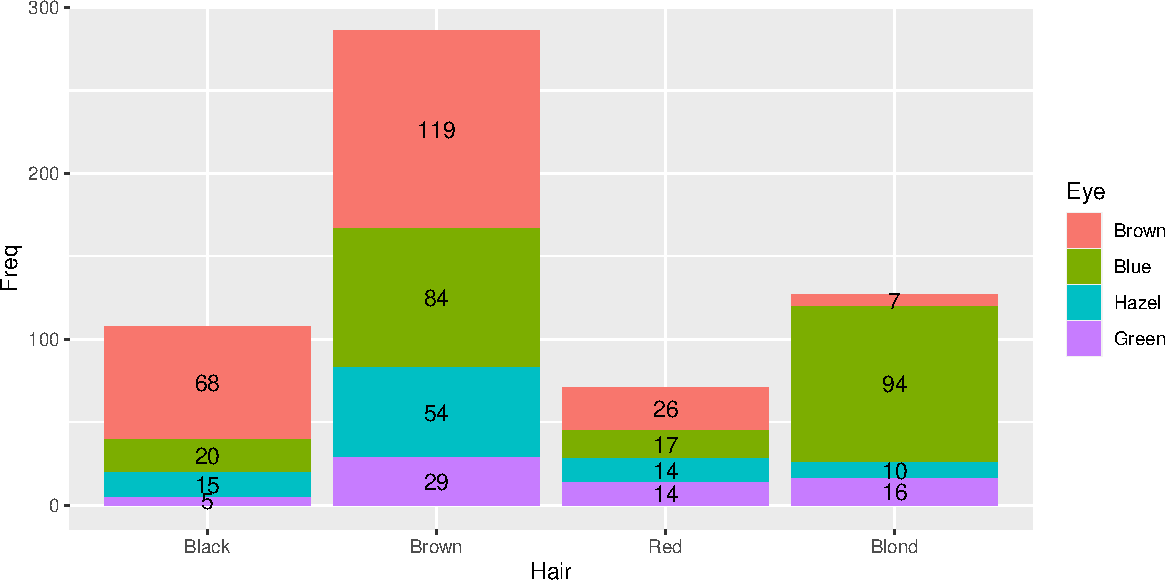
\includegraphics{inferencia_com_R_files/figure-latex/unnamed-chunk-26-1} \end{center}

A ordem dos grupos pode ser qualquer, ou aquela mais adequada para a presente análise. Frequentemente, encontramos as barras em ordem decrescente, já antecipando nossa intuição de ordenar os grupos de acordo com sua frequência para facilitar as comparações. Caso a variável fosse do tipo ordinal, a ordem das barras seria a ordem natural das categorias, como na tabela de frequências.

A figura abaixo mostra um gráfico de barras que pode ser usado da comparação da distribuição de frequências de uma mesma variável em vários grupos. É também uma alternativa ao uso de vários gráficos de setores, sendo, na verdade, a junção de dois gráficos com os das figuras acima num só gráfico. Porém, esse tipo de gráfico só deve ser usado quando não houver muitos grupos a serem comparados e a variável em estudo não tiver muitas categorias.

\begin{Shaded}
\begin{Highlighting}[]
\NormalTok{df }\OtherTok{=} \FunctionTok{data.frame}\NormalTok{(HairEyeColor[,,}\DecValTok{1}\NormalTok{] }\SpecialCharTok{+}\NormalTok{ HairEyeColor[,,}\DecValTok{2}\NormalTok{])}
\FunctionTok{ggplot}\NormalTok{(df,}\FunctionTok{aes}\NormalTok{(}\AttributeTok{x=}\NormalTok{Hair, }\AttributeTok{y=}\NormalTok{Freq, }\AttributeTok{fill=}\NormalTok{Eye)) }\SpecialCharTok{+}
  \FunctionTok{geom\_bar}\NormalTok{(}\AttributeTok{stat=}\StringTok{"identity"}\NormalTok{) }\SpecialCharTok{+}
  \FunctionTok{geom\_text}\NormalTok{(}\FunctionTok{aes}\NormalTok{(}\AttributeTok{label =}\NormalTok{ Freq),}\AttributeTok{position=}\FunctionTok{position\_stack}\NormalTok{(}\AttributeTok{vjust =} \FloatTok{0.5}\NormalTok{))}
\end{Highlighting}
\end{Shaded}

\begin{center}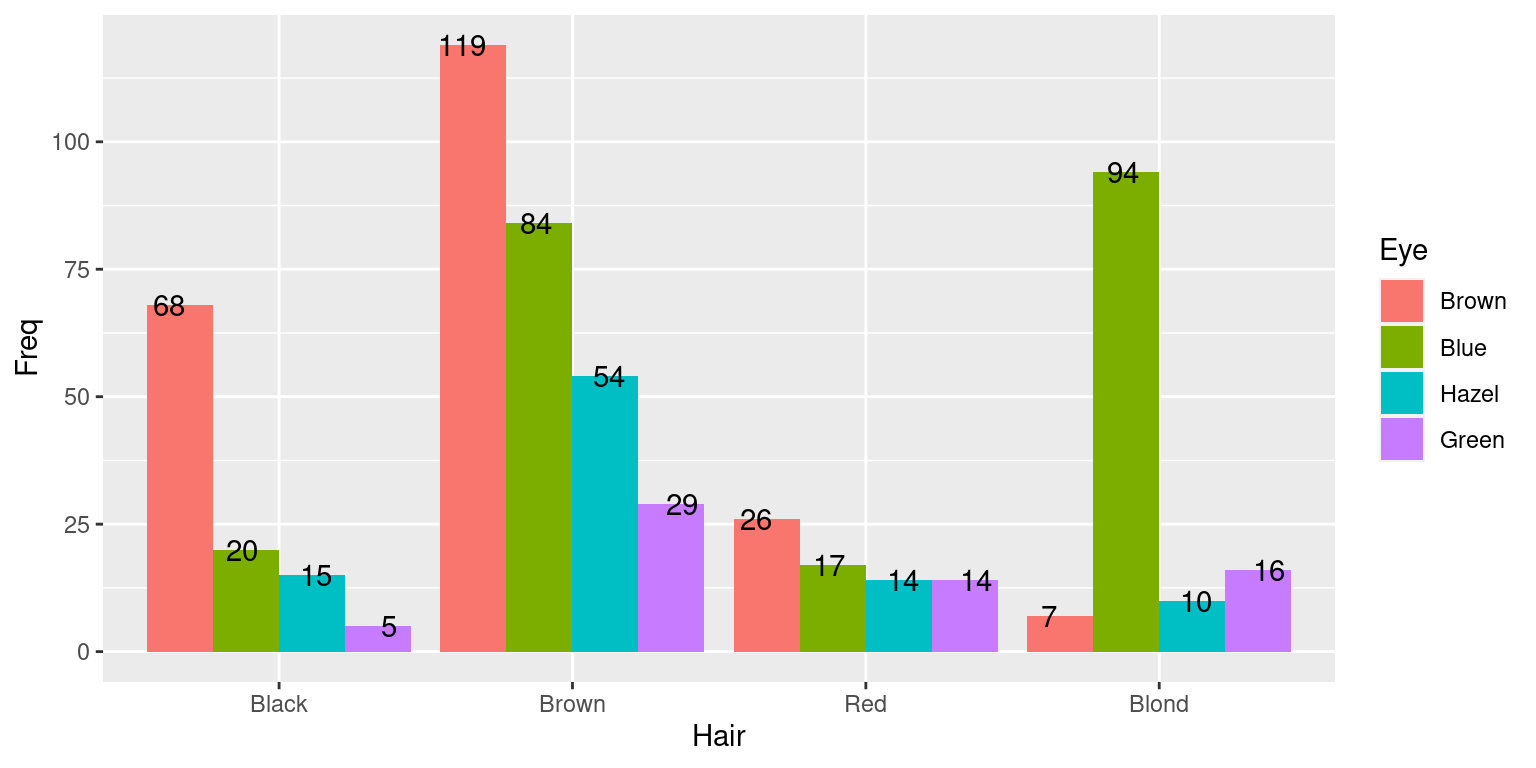
\includegraphics{inferencia_com_R_files/figure-latex/unnamed-chunk-27-1} \end{center}

Frequentemente, é necessário fazer comparações da distribuição de frequências de uma variável em vários grupos simultaneamente. Nesse caso, o uso de gráficos bem escolhidos e construídos torna a tarefa muito mais fácil. Na figura abaixo, está representada a distribuição de frequências da cor dos olhos segundo a variável cor do cabelo.

\begin{Shaded}
\begin{Highlighting}[]
\NormalTok{df }\OtherTok{=} \FunctionTok{data.frame}\NormalTok{(HairEyeColor[,,}\DecValTok{1}\NormalTok{] }\SpecialCharTok{+}\NormalTok{ HairEyeColor[,,}\DecValTok{2}\NormalTok{])}
\FunctionTok{ggplot}\NormalTok{(df,}\FunctionTok{aes}\NormalTok{(}\AttributeTok{x=}\NormalTok{Hair, }\AttributeTok{y=}\NormalTok{Freq, }\AttributeTok{fill=}\NormalTok{Eye)) }\SpecialCharTok{+}
  \FunctionTok{geom\_bar}\NormalTok{(}\AttributeTok{position=}\StringTok{"dodge"}\NormalTok{,}\AttributeTok{stat=}\StringTok{"identity"}\NormalTok{) }\SpecialCharTok{+}
  \FunctionTok{geom\_text}\NormalTok{(}\FunctionTok{aes}\NormalTok{(}\AttributeTok{label =}\NormalTok{ Freq),}\AttributeTok{position=}\FunctionTok{position\_dodge}\NormalTok{(}\AttributeTok{width =} \DecValTok{1}\NormalTok{))}
\end{Highlighting}
\end{Shaded}

\begin{center}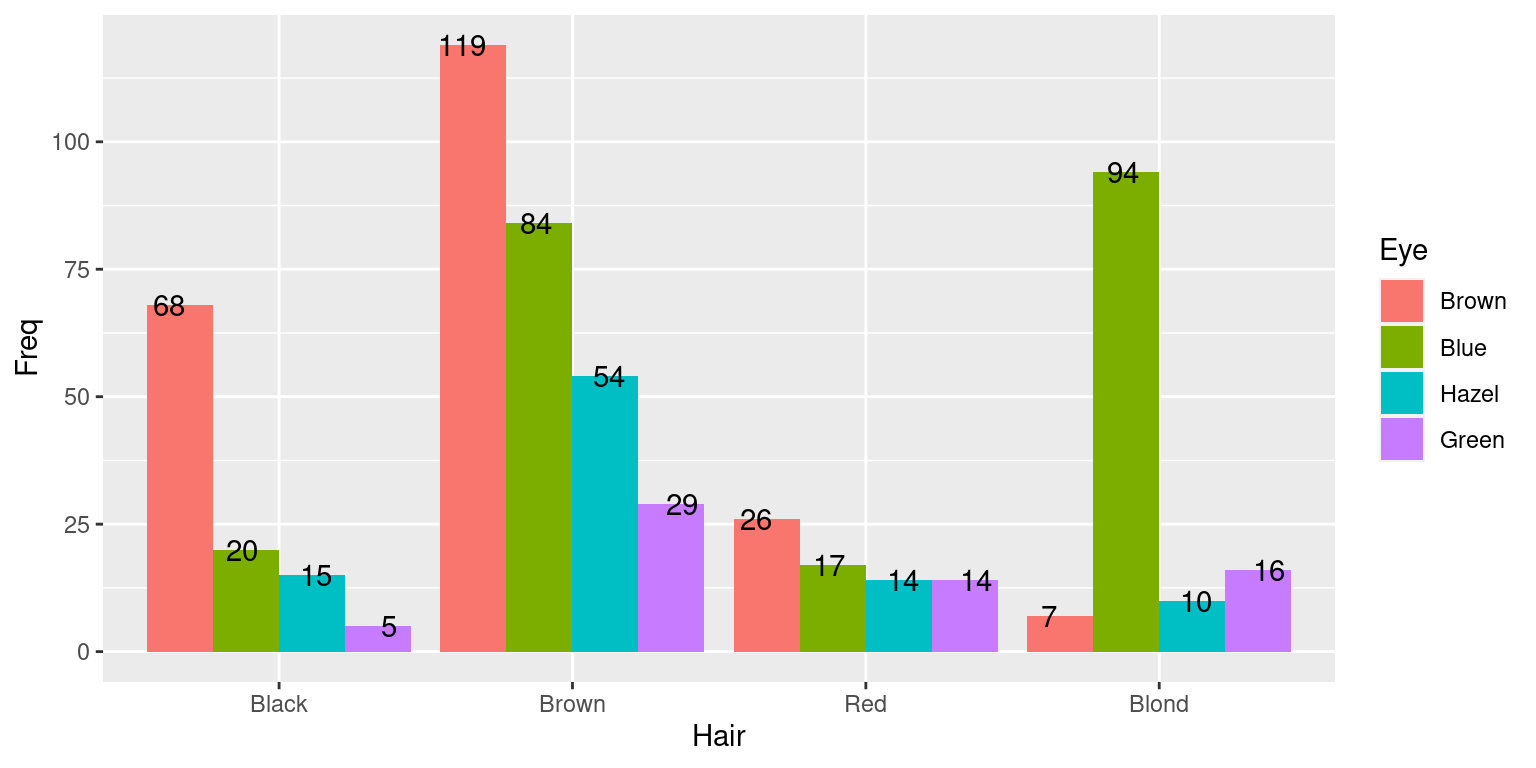
\includegraphics{inferencia_com_R_files/figure-latex/unnamed-chunk-28-1} \end{center}

\hypertarget{variuxe1veis-quantitativas-discretas}{%
\section{Variáveis Quantitativas Discretas}\label{variuxe1veis-quantitativas-discretas}}

Quando estamos trabalhando com uma variável discreta que assume poucos valores, podemos dar a ela o mesmo tratamento dado às variáveis qualitativas ordinais, assumindo que cada valor é uma classe e que existe uma ordem natural nessas classes.

Quando trabalhamos com uma variável discreta que pode assumir um grande número de valores distintos como, por exemplo, parte inteira da temperatura máxima, a construção da tabela de frequências e de gráficos considerando cada valor como uma categoria fica inviável. A solução é agrupar os valores em classes ao montar a tabela, como mostra a tabela abaixo.

\begin{tabular}{l>{\raggedleft\arraybackslash}p{2.5cm}>{\raggedleft\arraybackslash}p{2.5cm}>{\raggedright\arraybackslash}p{2.5cm}>{\raggedright\arraybackslash}p{2.5cm}}
\toprule
Temperatura & Frequência Absoluta & Frequência Relativa (\%) & Frequência Absoluta Acumulada & Frequência Relativa Acumulada (\%)\\
\midrule
56 a 67 & 21 & 15.67 & 21 & 15.67\\
67 a 78 & 47 & 35.07 & 68 & 50.75\\
78 a 89 & 66 & 49.25 & 134 & 100\\
Total & 134 & 99.99 & - & -\\
\bottomrule
\end{tabular}

A Figura abaixo mostra o gráfico da distribuição de frequências da temperatura medida por 236 dias consecutivos.

\begin{Shaded}
\begin{Highlighting}[]
\NormalTok{dt }\SpecialCharTok{\%\textgreater{}\%} \FunctionTok{filter}\NormalTok{(dt}\SpecialCharTok{$}\NormalTok{Variavel }\SpecialCharTok{!=} \StringTok{"Total"}\NormalTok{) }\SpecialCharTok{\%\textgreater{}\%} 
  \FunctionTok{ggplot}\NormalTok{(}\FunctionTok{aes}\NormalTok{(}\AttributeTok{x=}\NormalTok{Variavel, }\AttributeTok{y=}\NormalTok{Freq\_rel)) }\SpecialCharTok{+}
  \FunctionTok{geom\_bar}\NormalTok{(}\AttributeTok{position=}\StringTok{"dodge"}\NormalTok{,}\AttributeTok{stat=}\StringTok{"identity"}\NormalTok{) }\SpecialCharTok{+}
  \FunctionTok{labs}\NormalTok{(}\AttributeTok{x=}\StringTok{"Temperatura"}\NormalTok{,}\AttributeTok{y=}\StringTok{"Frequência Relativa (\%)"}\NormalTok{) }\SpecialCharTok{+}
  \FunctionTok{theme}\NormalTok{(}\AttributeTok{legend.position =} \StringTok{"none"}\NormalTok{)}
\end{Highlighting}
\end{Shaded}

\begin{center}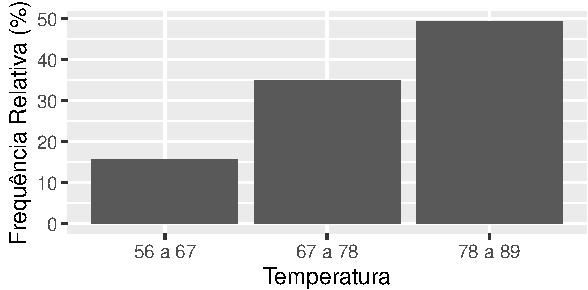
\includegraphics{inferencia_com_R_files/figure-latex/unnamed-chunk-30-1} \end{center}

\hypertarget{variuxe1veis-quantitativas-contuxednuas}{%
\section{Variáveis Quantitativas Contínuas}\label{variuxe1veis-quantitativas-contuxednuas}}

Quando a variável em estudo é do tipo contínua, que assume muitos valores distintos, o agrupamento dos dados em classes será sempre necessário na construção das tabelas de frequências. A tabela abaixo apresenta a distribuição de frequências para o peso dos carros.

\begin{tabular}{l>{\raggedleft\arraybackslash}p{2.5cm}>{\raggedleft\arraybackslash}p{2.5cm}>{\raggedright\arraybackslash}p{2.5cm}>{\raggedright\arraybackslash}p{2.5cm}}
\toprule
Temperatura & Frequência Absoluta & Frequência Relativa (\%) & Frequência Absoluta Acumulada & Frequência Relativa Acumulada (\%)\\
\midrule
1.5 |- 2 & 0 & 0.00 & 0 & 0\\
2 |- 2.5 & 0 & 0.00 & 0 & 0\\
2.5 |- 3 & 3 & 9.38 & 3 & 9.38\\
3 |- 3.5 & 10 & 31.25 & 13 & 40.62\\
3.5 |- 4 & 12 & 37.50 & 25 & 78.12\\
\addlinespace
4 |- 4.5 & 6 & 18.75 & 31 & 96.88\\
4.5 |- 5 & 1 & 3.12 & 32 & 100\\
5 |- 5.5 & 0 & 0.00 & 32 & 100\\
Total & 32 & 100.00 & - & -\\
\bottomrule
\end{tabular}

\hypertarget{histograma}{%
\section{Histograma}\label{histograma}}

A representação gráfica da distribuição de frequências de uma variável contínua é feita através de um gráfico chamado histograma, mostrado nas figuras abaixo com o peso de diamantes (\(\texttt{diamonds}\)). O histograma nada mais é do que o gráfico de barras verticais, porém construído com as barras unidas, devido ao caráter contínuo dos valores da variável.

\begin{Shaded}
\begin{Highlighting}[]
\FunctionTok{library}\NormalTok{(ggplot2)}
\NormalTok{p1}\OtherTok{=}\FunctionTok{ggplot}\NormalTok{(diamonds,}\FunctionTok{aes}\NormalTok{(carat)) }\SpecialCharTok{+}
  \FunctionTok{geom\_histogram}\NormalTok{(}\AttributeTok{color =} \StringTok{"white"}\NormalTok{) }\SpecialCharTok{+}
  \FunctionTok{labs}\NormalTok{(}\AttributeTok{y =} \StringTok{"Frequência Absoluta"}\NormalTok{)}
\NormalTok{p2}\OtherTok{=}\FunctionTok{ggplot}\NormalTok{(diamonds,}\FunctionTok{aes}\NormalTok{(carat)) }\SpecialCharTok{+}
  \FunctionTok{geom\_histogram}\NormalTok{(}\FunctionTok{aes}\NormalTok{(}\AttributeTok{y =}\NormalTok{ (..count..)}\SpecialCharTok{/}\FunctionTok{sum}\NormalTok{(..count..)}\SpecialCharTok{*}\DecValTok{100}\NormalTok{),}\AttributeTok{color =} \StringTok{"white"}\NormalTok{) }\SpecialCharTok{+}
  \FunctionTok{labs}\NormalTok{(}\AttributeTok{y =} \StringTok{"Frequência Relativa (\%)"}\NormalTok{)}
\NormalTok{gridExtra}\SpecialCharTok{::}\FunctionTok{grid.arrange}\NormalTok{(p1,p2,}\AttributeTok{ncol=}\DecValTok{2}\NormalTok{)}
\end{Highlighting}
\end{Shaded}

\begin{center}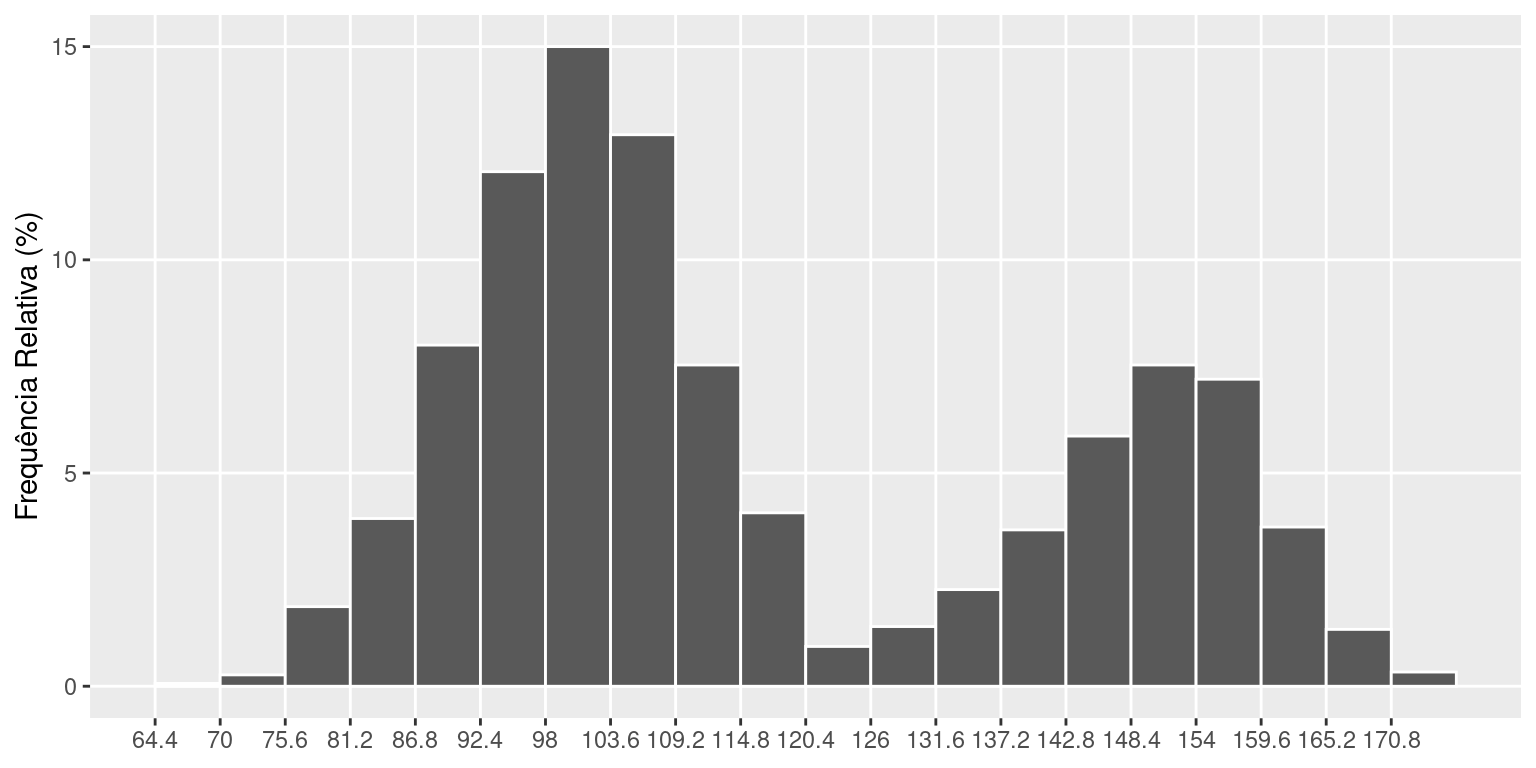
\includegraphics{inferencia_com_R_files/figure-latex/unnamed-chunk-32-1} \end{center}

Os histogramas das figuras acima têm exatamente a mesma forma, apesar de serem construídos usando as frequências absolutas e relativas, respectivamente. O objetivo dessas figuras é mostrar que a escolha do tipo de frequência a ser usada não muda a forma da distribuição. Entretanto, o uso da frequência relativa torna o histograma comparável a outros histogramas, mesmo que os conjuntos de dados tenham tamanhos diferentes (desde a mesma escala seja usada!)

Para o desenvolvimento do histograma:

\begin{itemize}
\tightlist
\item
  Calcule a amplitude dos dados
\item
  Defina a quantidade de classes (as barras verticais). Não existe uma regra, porém uma boa aproximação seria calcular a raiz quadrada da quantidade de dados (\(\sqrt n\))
\item
  Calcule o intervalo das classes dividindo a amplitude pela quantidade de classes
\item
  Determine os limites das classes. Selecione o valor mínimo dos dados (se for mais viável, ele pode ser arredondado para baixo) e soma o valor do intervalo de classe para obter o limite superior
\item
  Faça o passo anterior para todas as classes
\item
  Calcule a frequência dos dados que pertence a cada intervalo
\end{itemize}

Este é o passo a passo básico para a elaboração de um Histograma, que seja capaz de lhe trazer informações precisas sobre a frequência com que algo acontece em um determinado contexto.

Ao estudarmos a distribuição de frequências de uma variável quantitativa, seja em um grupo apenas ou comparando vários grupos, devemos verificar basicamente três características:

\begin{itemize}
\tightlist
\item
  Tendência Central;
\item
  Variabilidade;
\item
  Forma.
\end{itemize}

Tais características podem ser quantificadas através das medidas de síntese numérica ou visualizadas a partir do histograma.

\hypertarget{tenduxeancia-central}{%
\subsection{Tendência Central}\label{tenduxeancia-central}}

A tendência central da distribuição de frequências de uma variável é caracterizada pelo valor (ou faixa de valores) ``típico'' da variável.

Uma das maneiras de representar o que é ``típico'' é através do valor mais frequente da variável, chamado de moda. Ou, no caso da tabela de frequências, a classe de maior frequência, chamada de classe modal. No histograma, esta classe corresponde àquela com barra mais alta (``pico'').

\begin{center}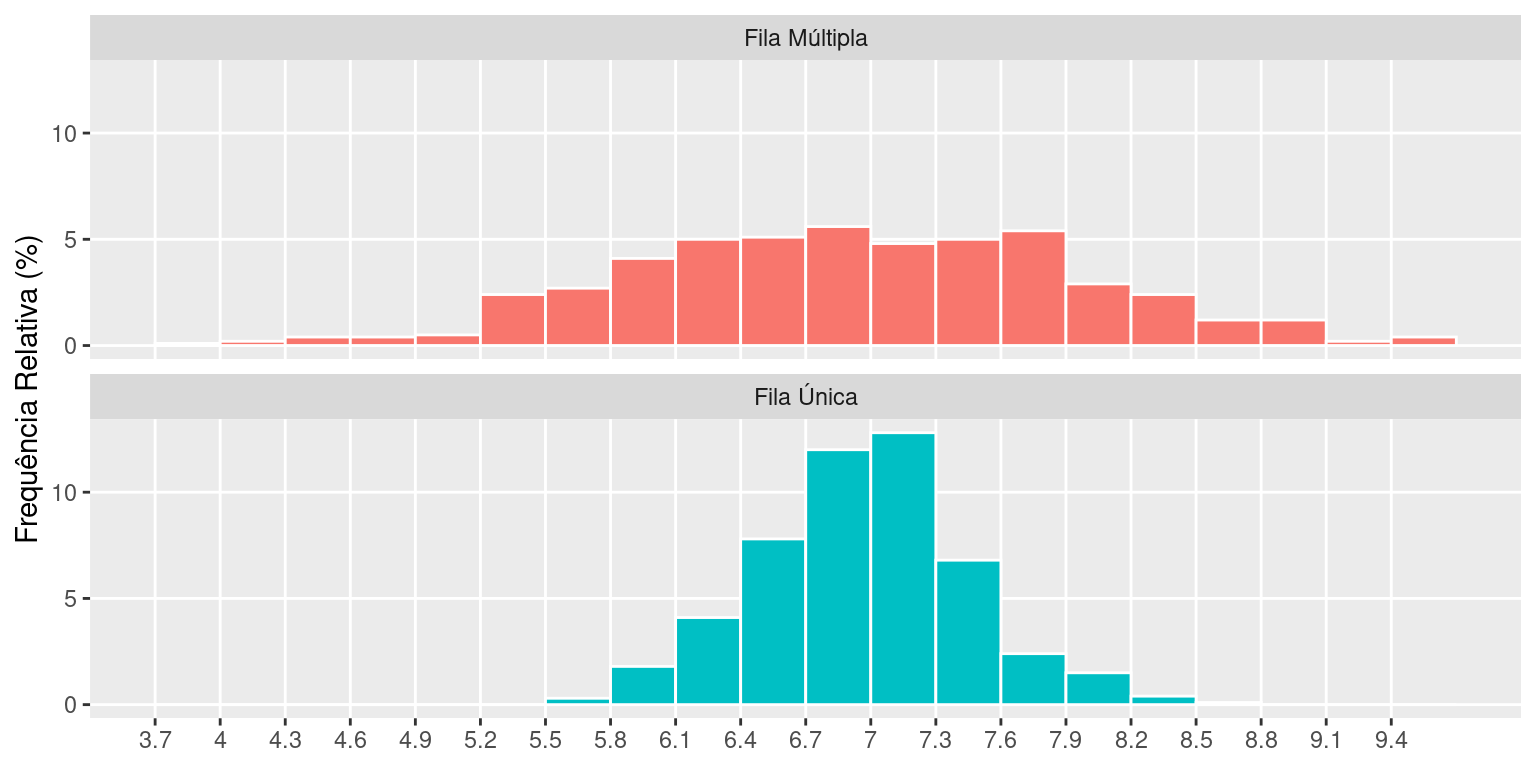
\includegraphics{inferencia_com_R_files/figure-latex/unnamed-chunk-33-1} \end{center}

No exemplo acima, a classe modal é a que vai de 97.9 até 103.5. Assim, os dados repousam, tipicamente entre esses valores. Entretanto, temos dois picos.

Geralmente, um histograma bimodal indica a existência de dois grupos, com valores centrados em dois pontos diferentes do eixo de valores. Uma distribuição de frequências pode também ser amodal, ou seja, todos os valores são igualmente frequentes. Ou também unimodal, quando os valores estão concentrados somente em um ponto/classe.

\hypertarget{variabilidade}{%
\subsection{Variabilidade}\label{variabilidade}}

Para descrever adequadamente a distribuição de frequências de uma variável quantitativa, além da informação do valor representativo da variável (tendência central), é necessário dizer também o quanto estes valores variam, ou seja, o quão dispersos eles são.

De fato, somente a informação sobre a tendência central de um conjunto de dados não consegue representá-lo adequadamente. A Figura abaixo mostra um histograma para os tempos de espera de 1000 clientes de dois bancos, um com fila única e outro com fila múltipla, com o mesmo número de atendentes. Os tempos de espera nos dois bancos têm a mesma tendência central de 7 minutos. Entretanto, os dois conjuntos de dados são claramente diferentes, pois os valores são muito mais dispersos no banco com fila múltipla. Assim, quando entramos num fila única, esperamos ser atendidos em cerca de 7 minutos, com uma variação de, no máximo, meio minuto a mais ou a menos. Na fila múltipla, a variação é maior, indicando-se que tanto pode-se esperar muito mais ou muito menos que o valor típico de 7 minutos.

\begin{center}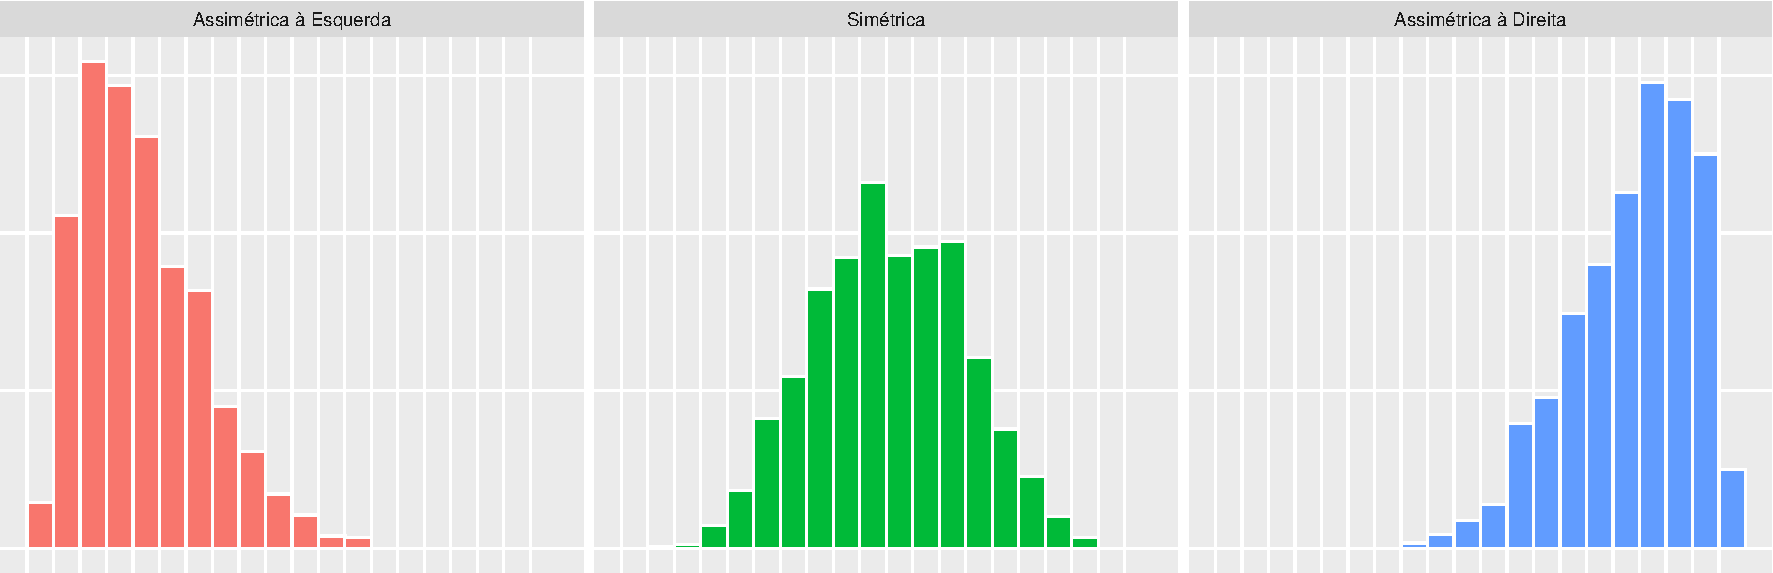
\includegraphics{inferencia_com_R_files/figure-latex/unnamed-chunk-34-1} \end{center}

\hypertarget{forma}{%
\subsection{Forma}\label{forma}}

A distribuição de frequências de uma variável pode ter várias formas, mas existem três formas básicas, apresentadas na figura abaixo através de histogramas.

\begin{center}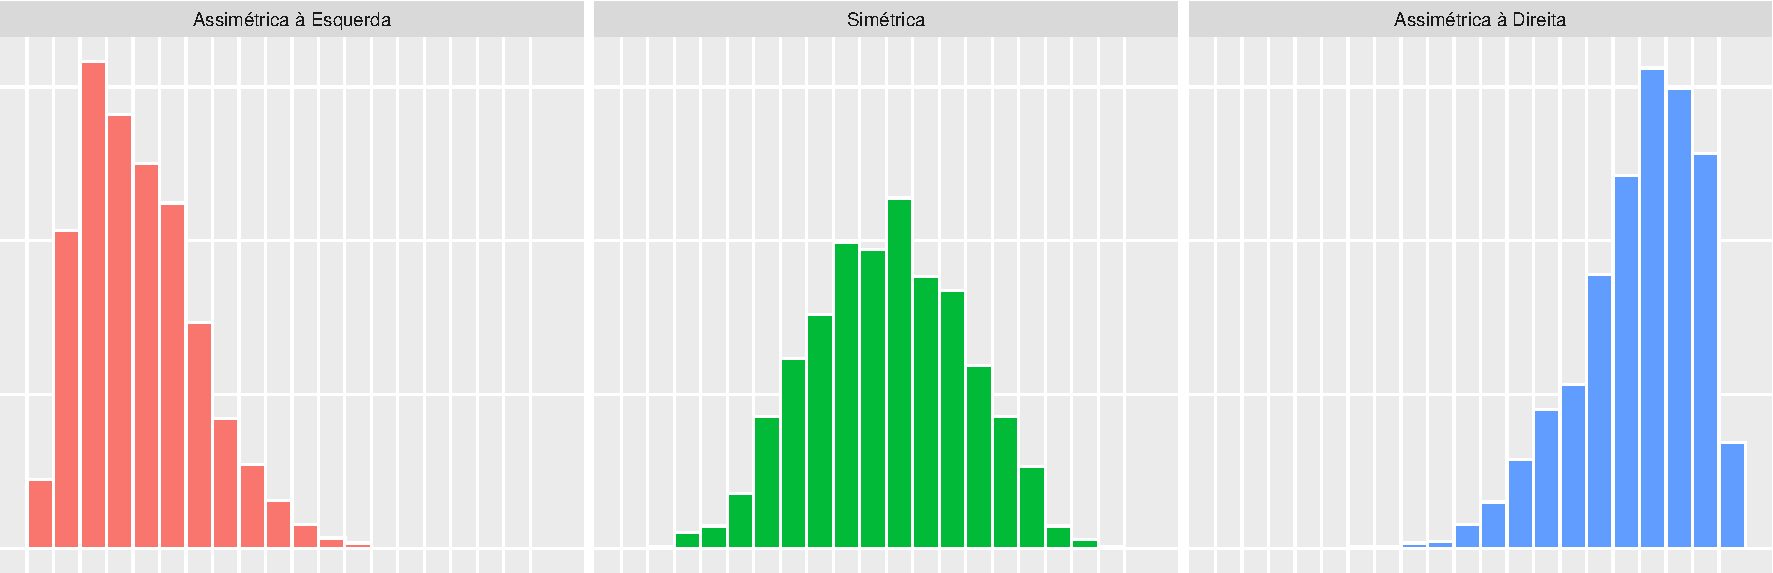
\includegraphics{inferencia_com_R_files/figure-latex/unnamed-chunk-35-1} \end{center}

Quando uma distribuição é simétrica em torno de um valor (o mais frequente), significa que as observações estão igualmente distribuídas em torno desse valor (metade acima e metade abaixo).

A assimetria de uma distribuição pode ocorrer de duas formas:

\begin{itemize}
\tightlist
\item
  quando os valores concentram-se à esquerda (assimetria com concentração à esquerda ou assimetria com cauda à direita);
\item
  quando os valores concentram-se à direita (assimetria com concentração à direita ou com assimetria cauda à esquerda);
\end{itemize}

Ao definir a assimetria de uma distribuição, algumas pessoas preferem se referir ao lado onde está a concentração dos dados. Porém, outras pessoas preferem se referir ao lado onde está ``faltando'' dados (cauda). As duas denominações são alternativas.

Em alguns casos, apenas o conhecimento da forma da distribuição de frequências de uma variável já nos fornece uma boa informação sobre o comportamento dessa variável. Por exemplo, o que você acharia se soubesse que a distribuição de frequências das notas da primeira prova da disciplina de Estatística que você está cursando é, geralmente, assimétrica com concentração à direita? Como você acha que é a forma da distribuição de frequências da renda no Brasil?

\hypertarget{boxplot}{%
\section{Boxplot}\label{boxplot}}

O Boxplot é um gráfico proposto para a detecção de valores discrepantes (outliers), que são aqueles valores muito diferentes do restante do conjunto de dados.

Esses valores discrepantes podem representar erros no processo de coleta ou de processamento dos dados, e, nesse caso, devem ser corrigidos ou excluídos do banco de dados. No entanto, os outliers podem ser valores corretos, que, por alguma razão, são muito diferentes dos demais valores. Nesse caso, a análise desses dados deve ser cuidadosa, pois, como sabemos, algumas estatísticas descritivas, como a média e o desvio-padrão, são influenciadas por valores extremos.

Na construção do Boxplot, utilizamos alguns percentis (mediana, primeiro e terceiro quartis), que são pouco influenciados por valores extremos. Além disso, precisamos saber quais são os valores mínimo e máximo do conjunto de dados.

O Boxplot é constituído por uma caixa atravessada por uma linha, construído usando um eixo com uma escala de valores, como mostra a figura abaixo. Como sabemos, entre o primeiro e o terceiro quartis, temos 50\% dos dados. Podemos pensar, então, que essa caixa contém metade dos dados do conjunto.

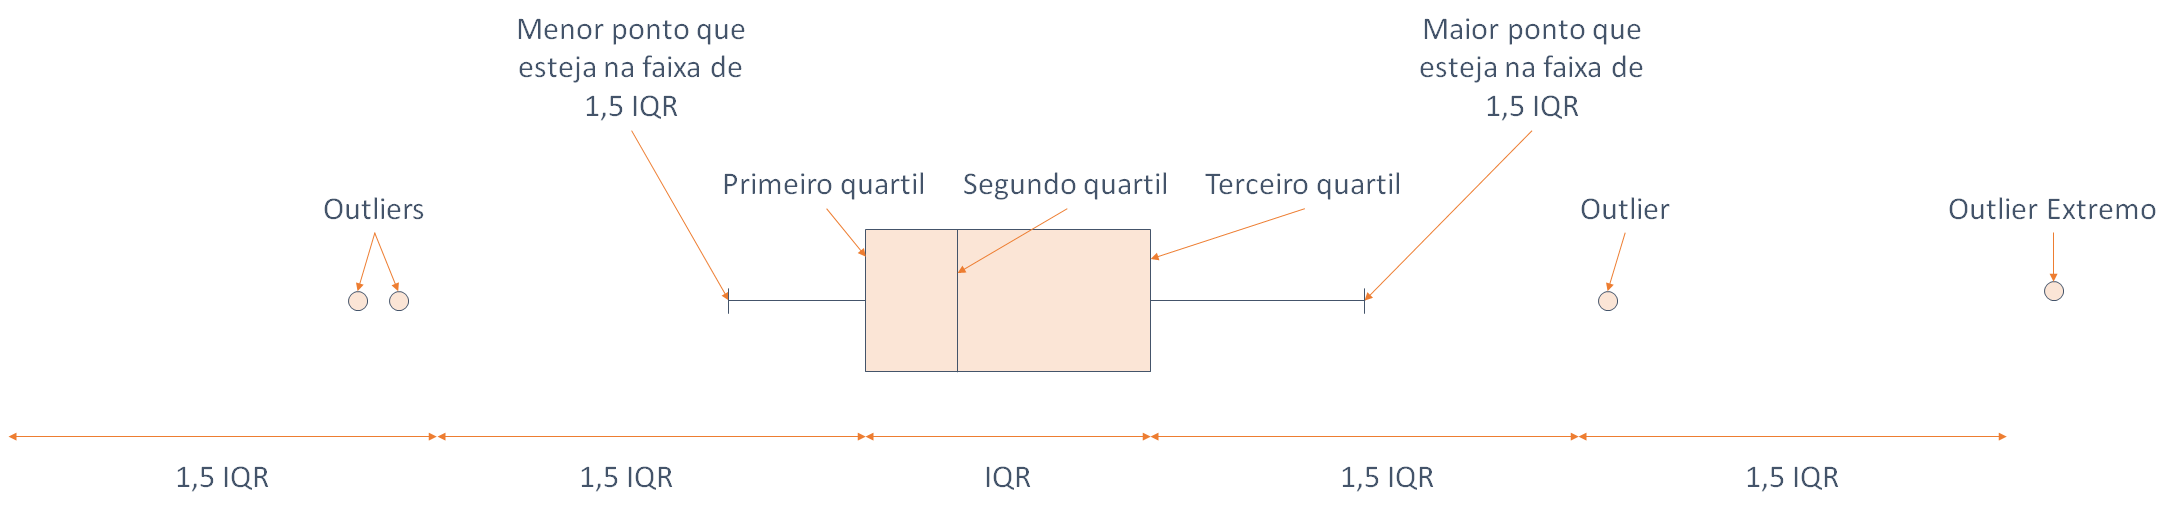
\includegraphics{Boxplot exemplo.png}

Como um gráfico tem que representar todos os valores do conjunto de dados, precisamos representar os outros 50\%, sendo 25\% abaixo do Q1 e 25\% acima do Q3. Esses valores serão representados pelas duas linhas que saem das extremidades da caixa. Cada uma das linhas é traçada, a partir das extremidades da caixa, até que encontre o valor máximo ou mínimo; ou atinja o comprimento máximo de 1,5 vezes a altura da caixa (IQR). O que acontecer primeiro.

No exemplo da imagem acima o segundo caso aconteceu, assim os valores que ainda não foram representados devem ser devidamente marcados em suas respectivas posições na escala de valores. Esses valores são considerados outliers pelo critério do boxplot. Obviamente, o limite superior do boxplot não coincidiu com o valor máximo do conjunto de dados, que foi considerado um valor discrepante (outlier).

Além da detecção de valores discrepantes, o boxplot pode ser muito útil na análise da distribuição dos valores de um conjunto de dados. Através do boxplot, podemos:

\begin{itemize}
\tightlist
\item
  identificar a forma da distribuição (simétrica ou assimétrica);
\item
  avaliar e comparar a tendência central (mediana) de dois ou mais conjuntos de dados;
\item
  comparar a variabilidade de dois ou mais conjuntos de dados
\end{itemize}

Para avaliar a forma da distribuição, devemos observar o deslocamento da caixa em relação a linha do boxplot. Lembrando que a caixa do boxplot contém 50\% dos dados, o seu deslocamento na linha nos informa onde estão concentrados os dados.

Se a caixa está mais deslocada para um dos lados da linha, significa que metade dos dados estão concentrados naquele lado da escala de valores e, assim, a distribuição é assimétrica. Se a caixa está praticamente no meio da linha, dividindo-a em duas partes iguais, é distribuição será considerada simétrica.

\begin{center}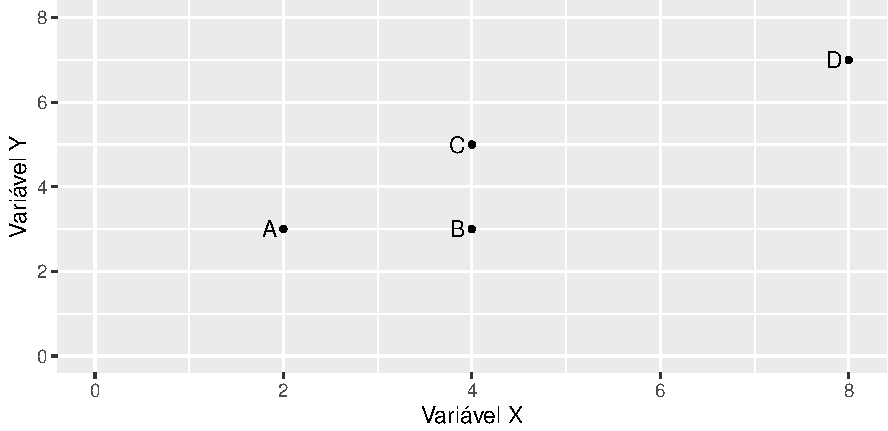
\includegraphics{inferencia_com_R_files/figure-latex/unnamed-chunk-37-1} \end{center}

\hypertarget{diagrama-de-dispersuxe3o}{%
\section{Diagrama de Dispersão}\label{diagrama-de-dispersuxe3o}}

O diagrama de dispersão é um gráfico onde pontos no espaço cartesiano XY são usados para representar simultaneamente os valores de duas variáveis quantitativas medidas em cada indivíduo do conjunto de dados.

O Quadro e a Figura abaixo mostram um esquema do desenho do diagrama de dispersão. Neste exemplo, foram medidos os valores de duas variáveis quantitativas, X e Y, em quatro indivíduos. O eixo horizontal do gráfico representa a variável X e o eixo vertical representa a variável Y.

\begin{tabular}{l>{\raggedleft\arraybackslash}p{2.5cm}>{\raggedleft\arraybackslash}p{2.5cm}>{}p{2.5cm}>{}p{2.5cm}}
\toprule
Indivíduos & Variável X & Variável Y\\
\midrule
A & 2 & 3\\
B & 4 & 3\\
C & 4 & 5\\
D & 8 & 7\\
\bottomrule
\end{tabular}

\begin{center}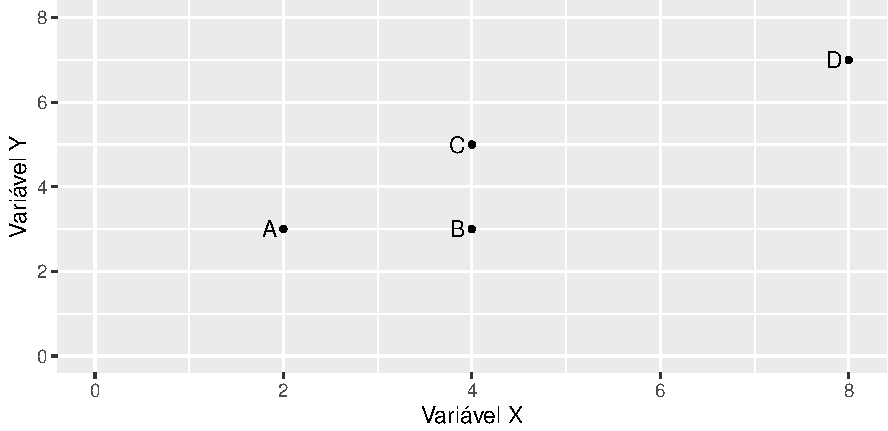
\includegraphics{inferencia_com_R_files/figure-latex/unnamed-chunk-38-1} \end{center}

O diagrama de dispersão é usado principalmente para visualizar a relação/associação entre duas variáveis, mas também para é muito útil para:

\begin{itemize}
\tightlist
\item
  Comparar o efeito de dois tratamentos no mesmo indivíduo
\item
  Verificar o efeito tipo antes/depois de um tratamento
\end{itemize}

A seguir, veremos dois exemplos da utilização do diagrama de dispersão. O primeiro refere-se ao estudo da associação entre duas variáveis. O segundo utiliza o diagrama de dispersão para comparar o efeito da aplicação de um tratamento, comparando as medidas antes e depois da medicação.

\hypertarget{exemplo-1}{%
\subsection{Exemplo 1}\label{exemplo-1}}

Um produtor de morangos para exportação deseja produzir frutos grandes, pois frutos pequenos têm pouco valor mesmo no mercado interno. Além disso, os frutos, mesmo grandes, não devem ter tamanhos muito diferentes entre si. O produtor suspeita que uma dos fatores que altera o tamanho dos frutos é o número de frutos por árvore.

Para investigar a relação entre o número de frutos que uma planta produz e o peso destes frutos, ele observou dados de 10 morangueiros na primeira safra (Quadro abaixo) e gerou o Diagrama de Dispersão apresentado abaixo.

\begin{table}
\centering\begingroup\fontsize{5}{7}\selectfont

\begin{tabular}{>{\raggedleft\arraybackslash}p{0.7cm}>{\raggedleft\arraybackslash}p{0.7cm}>{\raggedleft\arraybackslash}p{0.7cm}>{\raggedleft\arraybackslash}p{0.7cm}>{\raggedleft\arraybackslash}p{0.7cm}>{\raggedleft\arraybackslash}p{0.7cm}>{\raggedleft\arraybackslash}p{0.7cm}>{\raggedleft\arraybackslash}p{0.7cm}>{\raggedleft\arraybackslash}p{0.7cm}>{\raggedleft\arraybackslash}p{0.7cm}>{\raggedleft\arraybackslash}p{0.7cm}>{\raggedleft\arraybackslash}p{0.7cm}>{\raggedleft\arraybackslash}p{0.7cm}>{\raggedleft\arraybackslash}p{0.7cm}>{\raggedleft\arraybackslash}p{0.7cm}>{\raggedleft\arraybackslash}p{0.7cm}}
\toprule
Planta & Quantidade &  &  &  &  &  &  &  &  &  &  &  &  &  & \\
\midrule
1001 & 5 & 15.15 & 15.45 & 15.63 & 15.65 & 16.38 & NA & NA & NA & NA & NA & NA & NA & NA & NA\\
1002 & 6 & 14.00 & 14.50 & 15.35 & 15.86 & 15.94 & 16.13 & NA & NA & NA & NA & NA & NA & NA & NA\\
1003 & 7 & 13.67 & 13.76 & 14.06 & 14.11 & 14.54 & 14.89 & 15.50 & NA & NA & NA & NA & NA & NA & NA\\
1004 & 8 & 11.00 & 11.50 & 12.39 & 12.39 & 12.90 & 14.50 & 15.50 & 16.56 & NA & NA & NA & NA & NA & NA\\
1005 & 9 & 10.24 & 11.12 & 12.05 & 12.37 & 13.48 & 13.80 & 14.04 & 15.39 & 16.00 & NA & NA & NA & NA & NA\\
\addlinespace
1006 & 10 & 9.00 & 9.32 & 10.67 & 11.56 & 11.67 & 12.56 & 12.83 & 12.84 & 13.43 & 15.09 & NA & NA & NA & NA\\
1007 & 11 & 7.82 & 8.56 & 8.74 & 9.57 & 11.08 & 11.92 & 12.13 & 12.50 & 14.14 & 14.20 & 14.00 & NA & NA & NA\\
1008 & 12 & 7.25 & 9.41 & 10.15 & 10.33 & 10.80 & 10.95 & 11.13 & 11.48 & 11.49 & 12.86 & 13.37 & 15.04 & NA & NA\\
1009 & 13 & 6.95 & 7.61 & 8.53 & 10.00 & 10.94 & 11.04 & 11.43 & 11.63 & 11.97 & 12.02 & 12.74 & 13.53 & 14.00 & NA\\
1010 & 14 & 7.00 & 8.00 & 9.00 & 10.00 & 10.00 & 10.50 & 11.00 & 11.16 & 11.17 & 11.70 & 12.45 & 12.89 & 13.47 & 13.54\\
\bottomrule
\end{tabular}
\endgroup{}
\end{table}

\begin{Shaded}
\begin{Highlighting}[]
\FunctionTok{library}\NormalTok{(ggplot2)}
\FunctionTok{library}\NormalTok{(tidyr)}
\NormalTok{aux }\OtherTok{=} \FunctionTok{matrix}\NormalTok{(}\FunctionTok{c}\NormalTok{(}\FloatTok{15.15}\NormalTok{,}\FloatTok{15.45}\NormalTok{,}\FloatTok{15.63}\NormalTok{,}\FloatTok{15.65}\NormalTok{,}\FloatTok{16.38}\NormalTok{,}\ConstantTok{NA}\NormalTok{,}\ConstantTok{NA}\NormalTok{,}\ConstantTok{NA}\NormalTok{,}\ConstantTok{NA}\NormalTok{,}\ConstantTok{NA}\NormalTok{,}\ConstantTok{NA}\NormalTok{,}\ConstantTok{NA}\NormalTok{,}\ConstantTok{NA}\NormalTok{,}\ConstantTok{NA}\NormalTok{,}
               \DecValTok{14}\NormalTok{,}\FloatTok{14.5}\NormalTok{,}\FloatTok{15.35}\NormalTok{,}\FloatTok{15.86}\NormalTok{,}\FloatTok{15.94}\NormalTok{,}\FloatTok{16.13}\NormalTok{,}\ConstantTok{NA}\NormalTok{,}\ConstantTok{NA}\NormalTok{,}\ConstantTok{NA}\NormalTok{,}\ConstantTok{NA}\NormalTok{,}\ConstantTok{NA}\NormalTok{,}\ConstantTok{NA}\NormalTok{,}\ConstantTok{NA}\NormalTok{,}\ConstantTok{NA}\NormalTok{,}
               \FloatTok{13.67}\NormalTok{,}\FloatTok{13.76}\NormalTok{,}\FloatTok{14.06}\NormalTok{,}\FloatTok{14.11}\NormalTok{,}\FloatTok{14.54}\NormalTok{,}\FloatTok{14.89}\NormalTok{,}\FloatTok{15.5}\NormalTok{,}\ConstantTok{NA}\NormalTok{,}\ConstantTok{NA}\NormalTok{,}\ConstantTok{NA}\NormalTok{,}\ConstantTok{NA}\NormalTok{,}\ConstantTok{NA}\NormalTok{,}\ConstantTok{NA}\NormalTok{,}\ConstantTok{NA}\NormalTok{,}
               \DecValTok{11}\NormalTok{,}\FloatTok{11.5}\NormalTok{,}\FloatTok{12.39}\NormalTok{,}\FloatTok{12.39}\NormalTok{,}\FloatTok{12.9}\NormalTok{,}\FloatTok{14.5}\NormalTok{,}\FloatTok{15.5}\NormalTok{,}\FloatTok{16.56}\NormalTok{,}\ConstantTok{NA}\NormalTok{,}\ConstantTok{NA}\NormalTok{,}\ConstantTok{NA}\NormalTok{,}\ConstantTok{NA}\NormalTok{,}\ConstantTok{NA}\NormalTok{,}\ConstantTok{NA}\NormalTok{,}
               \FloatTok{10.24}\NormalTok{,}\FloatTok{11.12}\NormalTok{,}\FloatTok{12.05}\NormalTok{,}\FloatTok{12.37}\NormalTok{,}\FloatTok{13.48}\NormalTok{,}\FloatTok{13.8}\NormalTok{,}\FloatTok{14.04}\NormalTok{,}\FloatTok{15.39}\NormalTok{,}\DecValTok{16}\NormalTok{,}\ConstantTok{NA}\NormalTok{,}\ConstantTok{NA}\NormalTok{,}\ConstantTok{NA}\NormalTok{,}\ConstantTok{NA}\NormalTok{,}\ConstantTok{NA}\NormalTok{,}
               \DecValTok{9}\NormalTok{,}\FloatTok{9.32}\NormalTok{,}\FloatTok{10.67}\NormalTok{,}\FloatTok{11.56}\NormalTok{,}\FloatTok{11.67}\NormalTok{,}\FloatTok{12.56}\NormalTok{,}\FloatTok{12.83}\NormalTok{,}\FloatTok{12.84}\NormalTok{,}\FloatTok{13.43}\NormalTok{,}\FloatTok{15.09}\NormalTok{,}\ConstantTok{NA}\NormalTok{,}\ConstantTok{NA}\NormalTok{,}\ConstantTok{NA}\NormalTok{,}\ConstantTok{NA}\NormalTok{,}
               \FloatTok{7.82}\NormalTok{,}\FloatTok{8.56}\NormalTok{,}\FloatTok{8.74}\NormalTok{,}\FloatTok{9.57}\NormalTok{,}\FloatTok{11.08}\NormalTok{,}\FloatTok{11.92}\NormalTok{,}\FloatTok{12.13}\NormalTok{,}\FloatTok{12.5}\NormalTok{,}\FloatTok{14.14}\NormalTok{,}\FloatTok{14.2}\NormalTok{,}\DecValTok{14}\NormalTok{,}\ConstantTok{NA}\NormalTok{,}\ConstantTok{NA}\NormalTok{,}\ConstantTok{NA}\NormalTok{,}
               \FloatTok{7.25}\NormalTok{,}\FloatTok{9.41}\NormalTok{,}\FloatTok{10.15}\NormalTok{,}\FloatTok{10.33}\NormalTok{,}\FloatTok{10.8}\NormalTok{,}\FloatTok{10.95}\NormalTok{,}\FloatTok{11.13}\NormalTok{,}\FloatTok{11.48}\NormalTok{,}\FloatTok{11.49}\NormalTok{,}\FloatTok{12.86}\NormalTok{,}\FloatTok{13.37}\NormalTok{,}\FloatTok{15.04}\NormalTok{,}\ConstantTok{NA}\NormalTok{,}\ConstantTok{NA}\NormalTok{,}
               \FloatTok{6.95}\NormalTok{,}\FloatTok{7.61}\NormalTok{,}\FloatTok{8.53}\NormalTok{,}\DecValTok{10}\NormalTok{,}\FloatTok{10.94}\NormalTok{,}\FloatTok{11.04}\NormalTok{,}\FloatTok{11.43}\NormalTok{,}\FloatTok{11.63}\NormalTok{,}\FloatTok{11.97}\NormalTok{,}\FloatTok{12.02}\NormalTok{,}\FloatTok{12.74}\NormalTok{,}\FloatTok{13.53}\NormalTok{,}\DecValTok{14}\NormalTok{,}\ConstantTok{NA}\NormalTok{,}
               \DecValTok{7}\NormalTok{,}\DecValTok{8}\NormalTok{,}\DecValTok{9}\NormalTok{,}\DecValTok{10}\NormalTok{,}\DecValTok{10}\NormalTok{,}\FloatTok{10.5}\NormalTok{,}\DecValTok{11}\NormalTok{,}\FloatTok{11.16}\NormalTok{,}\FloatTok{11.17}\NormalTok{,}\FloatTok{11.7}\NormalTok{,}\FloatTok{12.45}\NormalTok{,}\FloatTok{12.89}\NormalTok{,}\FloatTok{13.47}\NormalTok{,}\FloatTok{13.54}\NormalTok{),}
             \AttributeTok{nrow=}\DecValTok{10}\NormalTok{,}\AttributeTok{ncol =} \DecValTok{14}\NormalTok{,}\AttributeTok{byrow =}\NormalTok{ T)}
\NormalTok{dados }\OtherTok{=} \FunctionTok{data.frame}\NormalTok{(}\AttributeTok{ID\_Morangueiro =} \DecValTok{1001}\SpecialCharTok{:}\DecValTok{1010}\NormalTok{,}
                   \AttributeTok{Qtd\_Frutos =} \DecValTok{5}\SpecialCharTok{:}\DecValTok{14}\NormalTok{,aux)}
\NormalTok{dados }\SpecialCharTok{\%\textgreater{}\%} 
  \FunctionTok{pivot\_longer}\NormalTok{(}\FunctionTok{starts\_with}\NormalTok{(}\StringTok{"X"}\NormalTok{)) }\SpecialCharTok{\%\textgreater{}\%} 
  \FunctionTok{ggplot}\NormalTok{(}\FunctionTok{aes}\NormalTok{(}\AttributeTok{x =}\NormalTok{ Qtd\_Frutos, }\AttributeTok{y =}\NormalTok{ value)) }\SpecialCharTok{+}
  \FunctionTok{geom\_point}\NormalTok{(}\AttributeTok{size =} \DecValTok{1}\NormalTok{) }\SpecialCharTok{+}
  \FunctionTok{scale\_x\_discrete}\NormalTok{(}\AttributeTok{limits=}\DecValTok{5}\SpecialCharTok{:}\DecValTok{14}\NormalTok{) }\SpecialCharTok{+}
  \FunctionTok{labs}\NormalTok{(}\AttributeTok{x =} \StringTok{"Quantidade de Frutos"}\NormalTok{,}\AttributeTok{y =} \StringTok{"Peso do Fruto (g)"}\NormalTok{)}
\end{Highlighting}
\end{Shaded}

\begin{center}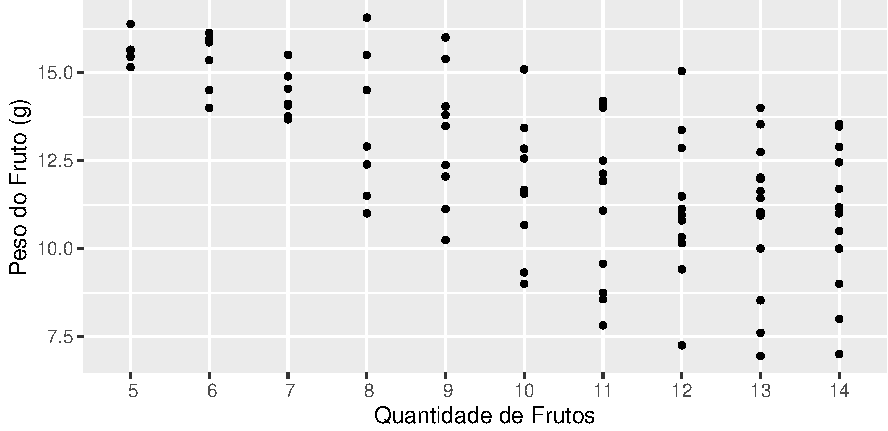
\includegraphics{inferencia_com_R_files/figure-latex/unnamed-chunk-41-1} \end{center}

O diagrama de dispersão mostra-nos dois fatos. O primeiro, que há um decréscimo no valor médio do peso do fruto por árvore à medida que cresce o número de frutos na árvore. Ou seja, não é vantagem uma árvore produzir muitos frutos, pois eles tenderão a ser muito pequenos.

O segundo fato que percebemos é que, com o aumento no número de frutos na árvore, cresce também a variabilidade no peso, gerando tanto frutos muito grandes, como muito pequenos.

Assim, conclui-se que não é vantagem ter poucas plantas produzindo muito frutos, mas sim muitas plantas produzindo poucos frutos, mas grandes e uniformes. Uma análise mais detalhada poderá determinar o número ideal de frutos por árvore, aquele que maximiza o peso médio e, ao mesmo tempo, minimiza a variabilidade do peso.

\hypertarget{exemplo-2}{%
\subsection{Exemplo 2}\label{exemplo-2}}

Captopril é um remédio destinado a baixar a pressão sistólica. Para testar seu efeito, ele foi ministrado a 12 pacientes, tendo sido medida a pressão sistólica antes e depois da medicação.

\begin{tabular}{l>{\raggedleft\arraybackslash}p{2.5cm}>{\raggedleft\arraybackslash}p{2.5cm}>{}p{2.5cm}>{}p{2.5cm}}
\toprule
Paciente & Antes & Depois\\
\midrule
A & 200 & 191\\
B & 174 & 170\\
C & 198 & 177\\
D & 170 & 167\\
E & 179 & 159\\
\addlinespace
F & 182 & 151\\
G & 193 & 176\\
H & 209 & 183\\
I & 185 & 159\\
J & 155 & 145\\
\addlinespace
K & 169 & 146\\
L & 210 & 177\\
\bottomrule
\end{tabular}

Os mesmos indivíduos foram utilizados nas duas amostras (Antes/depois). Assim, é natural compararmos a pressão sistólica para cada indivíduo, comparando a pressão sistólica depois e antes. Para todos os pacientes, a pressão sistólica depois do Captopril é menor do que antes da medicação. Mas como podemos ``ver'' se estas diferenças são grandes? Com a ajuda do diagrama de dispersão mostrado na figura abaixo.

\begin{Shaded}
\begin{Highlighting}[]
\NormalTok{dados }\OtherTok{=} \FunctionTok{data.frame}\NormalTok{(}\AttributeTok{Paciente =}\NormalTok{ LETTERS[}\DecValTok{1}\SpecialCharTok{:}\DecValTok{12}\NormalTok{],}
                   \AttributeTok{Antes =} \FunctionTok{c}\NormalTok{(}\DecValTok{200}\NormalTok{, }\DecValTok{174}\NormalTok{, }\DecValTok{198}\NormalTok{, }\DecValTok{170}\NormalTok{, }\DecValTok{179}\NormalTok{, }\DecValTok{182}\NormalTok{, }\DecValTok{193}\NormalTok{, }\DecValTok{209}\NormalTok{, }\DecValTok{185}\NormalTok{, }\DecValTok{155}\NormalTok{, }\DecValTok{169}\NormalTok{, }\DecValTok{210}\NormalTok{),}
                   \AttributeTok{Depois =} \FunctionTok{c}\NormalTok{(}\DecValTok{191}\NormalTok{, }\DecValTok{170}\NormalTok{, }\DecValTok{177}\NormalTok{, }\DecValTok{167}\NormalTok{, }\DecValTok{159}\NormalTok{, }\DecValTok{151}\NormalTok{, }\DecValTok{176}\NormalTok{, }\DecValTok{183}\NormalTok{, }\DecValTok{159}\NormalTok{, }\DecValTok{145}\NormalTok{, }\DecValTok{146}\NormalTok{, }\DecValTok{177}\NormalTok{))}

\NormalTok{dados }\SpecialCharTok{\%\textgreater{}\%}
  \FunctionTok{ggplot}\NormalTok{(}\FunctionTok{aes}\NormalTok{(}\AttributeTok{x =}\NormalTok{ Antes, }\AttributeTok{y =}\NormalTok{ Depois)) }\SpecialCharTok{+}
  \FunctionTok{geom\_point}\NormalTok{(}\AttributeTok{size =} \DecValTok{1}\NormalTok{) }\SpecialCharTok{+}
  \FunctionTok{ylim}\NormalTok{(}\DecValTok{140}\NormalTok{,}\DecValTok{220}\NormalTok{) }\SpecialCharTok{+} \FunctionTok{xlim}\NormalTok{(}\DecValTok{140}\NormalTok{,}\DecValTok{220}\NormalTok{) }\SpecialCharTok{+}
  \FunctionTok{geom\_abline}\NormalTok{(}\AttributeTok{slope =} \DecValTok{1}\NormalTok{, }\AttributeTok{intercept =} \DecValTok{0}\NormalTok{) }\SpecialCharTok{+}
  \FunctionTok{geom\_text}\NormalTok{(}\FunctionTok{aes}\NormalTok{(}\AttributeTok{x =} \DecValTok{200}\NormalTok{, }\AttributeTok{y =} \DecValTok{160}\NormalTok{), }\AttributeTok{label =} \StringTok{"Depois \textless{} Antes"}\NormalTok{) }\SpecialCharTok{+}
  \FunctionTok{geom\_text}\NormalTok{(}\FunctionTok{aes}\NormalTok{(}\AttributeTok{x =} \DecValTok{160}\NormalTok{, }\AttributeTok{y =} \DecValTok{200}\NormalTok{), }\AttributeTok{label =} \StringTok{"Depois \textgreater{} Antes"}\NormalTok{) }\SpecialCharTok{+}
  \FunctionTok{geom\_text}\NormalTok{(}\FunctionTok{aes}\NormalTok{(}\AttributeTok{x =} \DecValTok{210}\NormalTok{, }\AttributeTok{y =} \DecValTok{210}\NormalTok{), }\AttributeTok{label =} \StringTok{"Depois = Antes"}\NormalTok{)}
\end{Highlighting}
\end{Shaded}

\begin{center}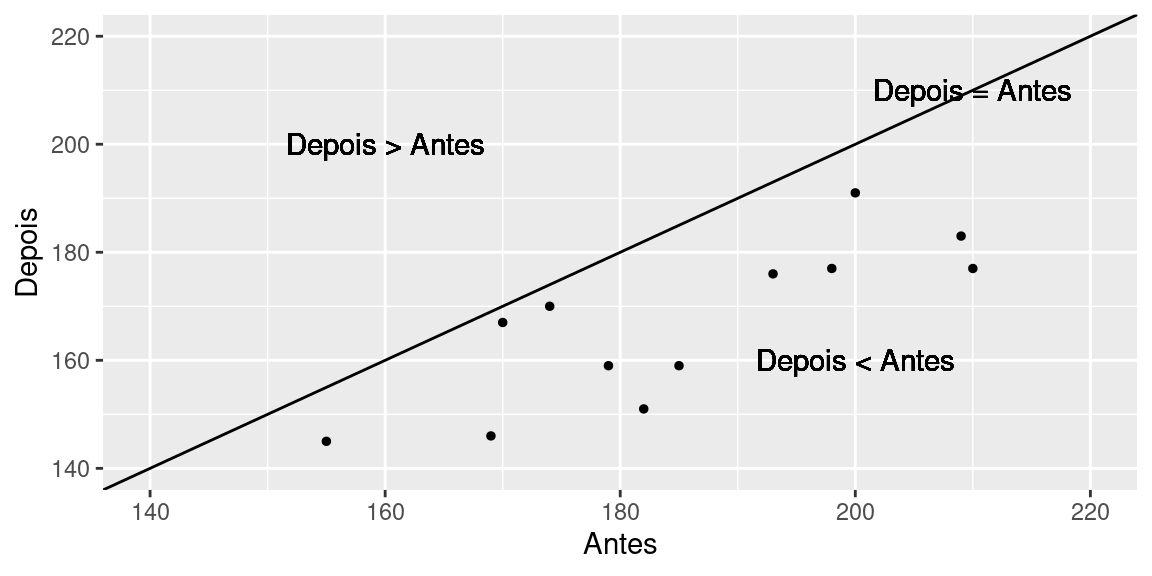
\includegraphics{inferencia_com_R_files/figure-latex/unnamed-chunk-43-1} \end{center}

Cada ponto no diagrama de dispersão corresponde às medidas de pressão sistólica de um paciente, medida antes e depois da medicação. A linha marcada no diagrama corresponde à situação onde a pressão sistólica não se alterou depois do paciente tomar o Captopril. Veja que todos os pontos estão abaixo desta linha, ou seja para todos os pacientes o Captopril fez efeito. Grande parte destes pontos está bem distante da linha, mostrando que a redução na pressão sistólica depois do uso do medicamento não foi pequena.

\hypertarget{suxe9ries-temporais}{%
\section{Séries Temporais}\label{suxe9ries-temporais}}

Séries temporais (ou séries históricas) são um conjunto de observações de uma mesma variável quantitativa (discreta ou contínua) feitas ao longo do tempo. O conjunto de novos casos da COVID-19 é um exemplo de série temporal.

Um dos objetivos do estudo de séries temporais é conhecer o comportamento da série ao longo do tempo (aumento, estabilidade ou declínio dos valores). Em alguns estudos, esse conhecimento pode ser usado para se fazer previsões de valores futuros com base no comportamento dos valores passados.

A representação gráfica de uma série temporal é feita através do gráfico de linha, como exemplificado nas figuras abaixo. No eixo horizontal do gráfico de linha, está o indicador de tempo e, no eixo vertical, a variável a ser representada.

\begin{Shaded}
\begin{Highlighting}[]
\FunctionTok{library}\NormalTok{(tsibble)}
\FunctionTok{library}\NormalTok{(lubridate)}
\FunctionTok{library}\NormalTok{(dplyr)}

\NormalTok{dados }\OtherTok{=} \FunctionTok{read.csv}\NormalTok{(}\StringTok{"https://raw.githubusercontent.com/wcota/covid19br/master/cases{-}brazil{-}states.csv"}\NormalTok{)}

\NormalTok{dados }\SpecialCharTok{\%\textgreater{}\%}
  \FunctionTok{mutate}\NormalTok{(}\AttributeTok{date =} \FunctionTok{as\_date}\NormalTok{(date)) }\SpecialCharTok{\%\textgreater{}\%} 
  \FunctionTok{as\_tsibble}\NormalTok{(}\AttributeTok{key =}\NormalTok{ state, }\AttributeTok{index =}\NormalTok{ date) }\SpecialCharTok{\%\textgreater{}\%} 
  \FunctionTok{filter}\NormalTok{(state }\SpecialCharTok{==} \StringTok{"TOTAL"}\NormalTok{) }\SpecialCharTok{\%\textgreater{}\%} 
  \FunctionTok{select}\NormalTok{(date, newCases) }\SpecialCharTok{\%\textgreater{}\%}
  \FunctionTok{ggplot}\NormalTok{(}\FunctionTok{aes}\NormalTok{(}\AttributeTok{x =}\NormalTok{ date, }\AttributeTok{y =}\NormalTok{ newCases)) }\SpecialCharTok{+}
  \FunctionTok{geom\_line}\NormalTok{() }\SpecialCharTok{+}
  \FunctionTok{labs}\NormalTok{(}\AttributeTok{title =} \StringTok{"Evolução dos casos de COVID{-}19 no Brasil"}\NormalTok{,}
       \AttributeTok{y =} \StringTok{"Novos Casos"}\NormalTok{, }\AttributeTok{x =} \StringTok{"Data"}\NormalTok{)}
\end{Highlighting}
\end{Shaded}

\begin{center}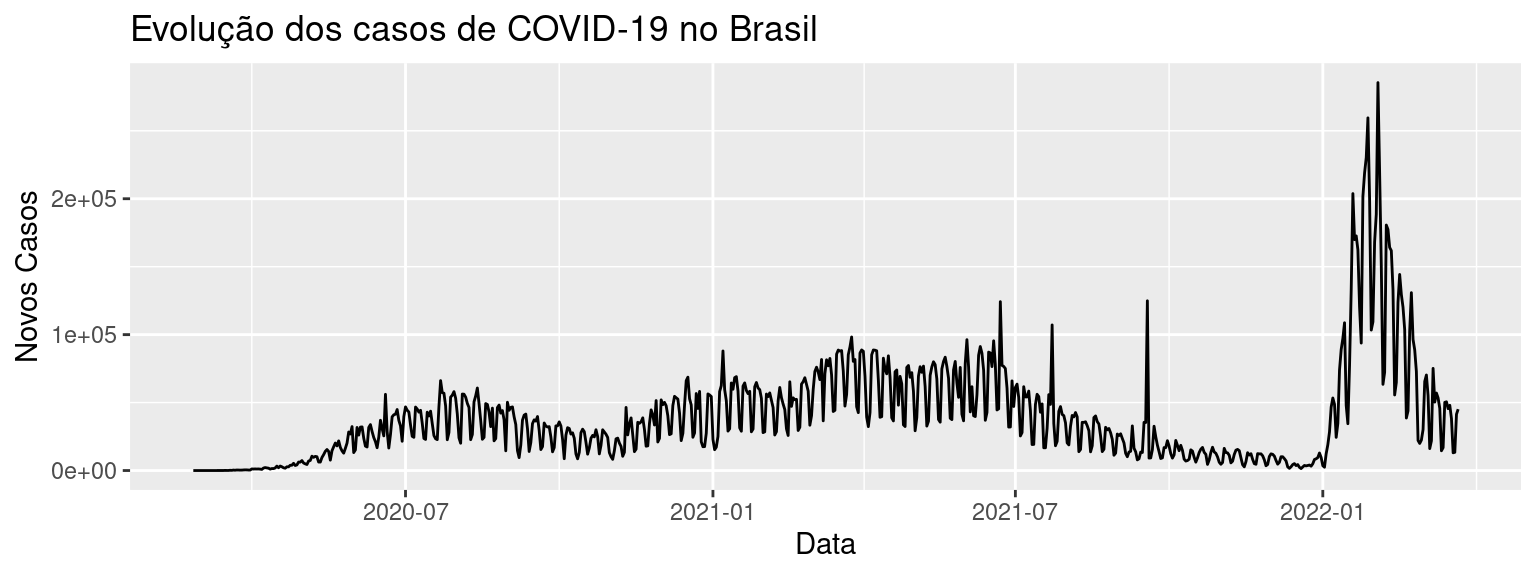
\includegraphics{inferencia_com_R_files/figure-latex/unnamed-chunk-44-1} \end{center}

De maneira geral, um gráfico de linhas deve ser construído de modo que:

\begin{itemize}
\tightlist
\item
  O início do eixo vertical seja o valor mínimo possível para a variável que está sendo representada, para evitar as distorções
\item
  O final do eixo vertical seja tal que a série fica centrada em relação ao eixo vertical
\item
  Os tamanhos dos eixos sejam o mais parecidos possível
\end{itemize}

\hypertarget{gruxe1fico-de-radar}{%
\section{Gráfico de Radar}\label{gruxe1fico-de-radar}}

O gráfico de radar é um diagrama e/ou gráfico que consiste de uma sequência de raios equi-angulares, com cada raio representando uma das variáveis. O comprimento de cada raio é proporcional à magnitude da variável para o ponto de dados em relação à máxima magnitude da variável em todos os pontos. Uma linha é desenhada ligando os valores de cada raio. Isso dá ao diagrama uma aparência de estrela, o que deu origem a um dos nomes mais populares para este gráfico. O gráfico de estrela pode ser usado para responder as seguintes questões:

\begin{itemize}
\tightlist
\item
  Que observações são mais semelhantes, por exemplo, existem clusters de observações?
\item
  Existem exceções?
\end{itemize}

Gráficos de radar oferecem uma maneira útil de exibir observações multivariáveis com um número arbitrário de variáveis. Cada estrela representa uma única observação. Normalmente, os gráficos de radar são gerados em um formato multi-diagrama com muitas estrelas em cada página, cada estrela representando uma observação. É um pouco mais fácil de ver padrões em dados se as observações forem organizadas em alguma ordem não-arbitrária (se as variáveis forem atribuídas aos raios da estrela em uma ordem significativa).

Uma aplicação de gráficos de radar é o controle de melhoria de qualidade para apresentar as métricas de desempenho de qualquer programa em curso. Eles também são usados em esportes para representar os pontos fortes e fracos de jogadores, onde eles são geralmente chamados de gráficos de aranha. No exemplo abaixo vemos a performance de três alunos (a,b,c) em relação as dimensões matemática, inglês, biologia, música e R.

\begin{Shaded}
\begin{Highlighting}[]
\FunctionTok{library}\NormalTok{(fmsb)}

\NormalTok{dados }\OtherTok{=} \FunctionTok{as.data.frame}\NormalTok{(}\FunctionTok{matrix}\NormalTok{(}\FunctionTok{sample}\NormalTok{(}\DecValTok{0}\SpecialCharTok{:}\DecValTok{20}\NormalTok{, }\DecValTok{15}\NormalTok{, }\AttributeTok{replace=}\NormalTok{F), }\AttributeTok{ncol=}\DecValTok{5}\NormalTok{))}
\FunctionTok{colnames}\NormalTok{(dados) }\OtherTok{=} \FunctionTok{c}\NormalTok{(}\StringTok{"matemática"}\NormalTok{, }\StringTok{"inglês"}\NormalTok{, }\StringTok{"biologia"}\NormalTok{, }\StringTok{"música"}\NormalTok{ ,}\StringTok{"R"}\NormalTok{)}
\FunctionTok{rownames}\NormalTok{(dados) }\OtherTok{=} \FunctionTok{paste}\NormalTok{(}\StringTok{"aluno"}\NormalTok{, letters[}\DecValTok{1}\SpecialCharTok{:}\DecValTok{3}\NormalTok{])}

\NormalTok{dados }\OtherTok{=} \FunctionTok{rbind}\NormalTok{(}\FunctionTok{rep}\NormalTok{(}\DecValTok{20}\NormalTok{,}\DecValTok{5}\NormalTok{), }\FunctionTok{rep}\NormalTok{(}\DecValTok{0}\NormalTok{,}\DecValTok{5}\NormalTok{), dados)}
 
\FunctionTok{radarchart}\NormalTok{(dados)}
\end{Highlighting}
\end{Shaded}

\begin{center}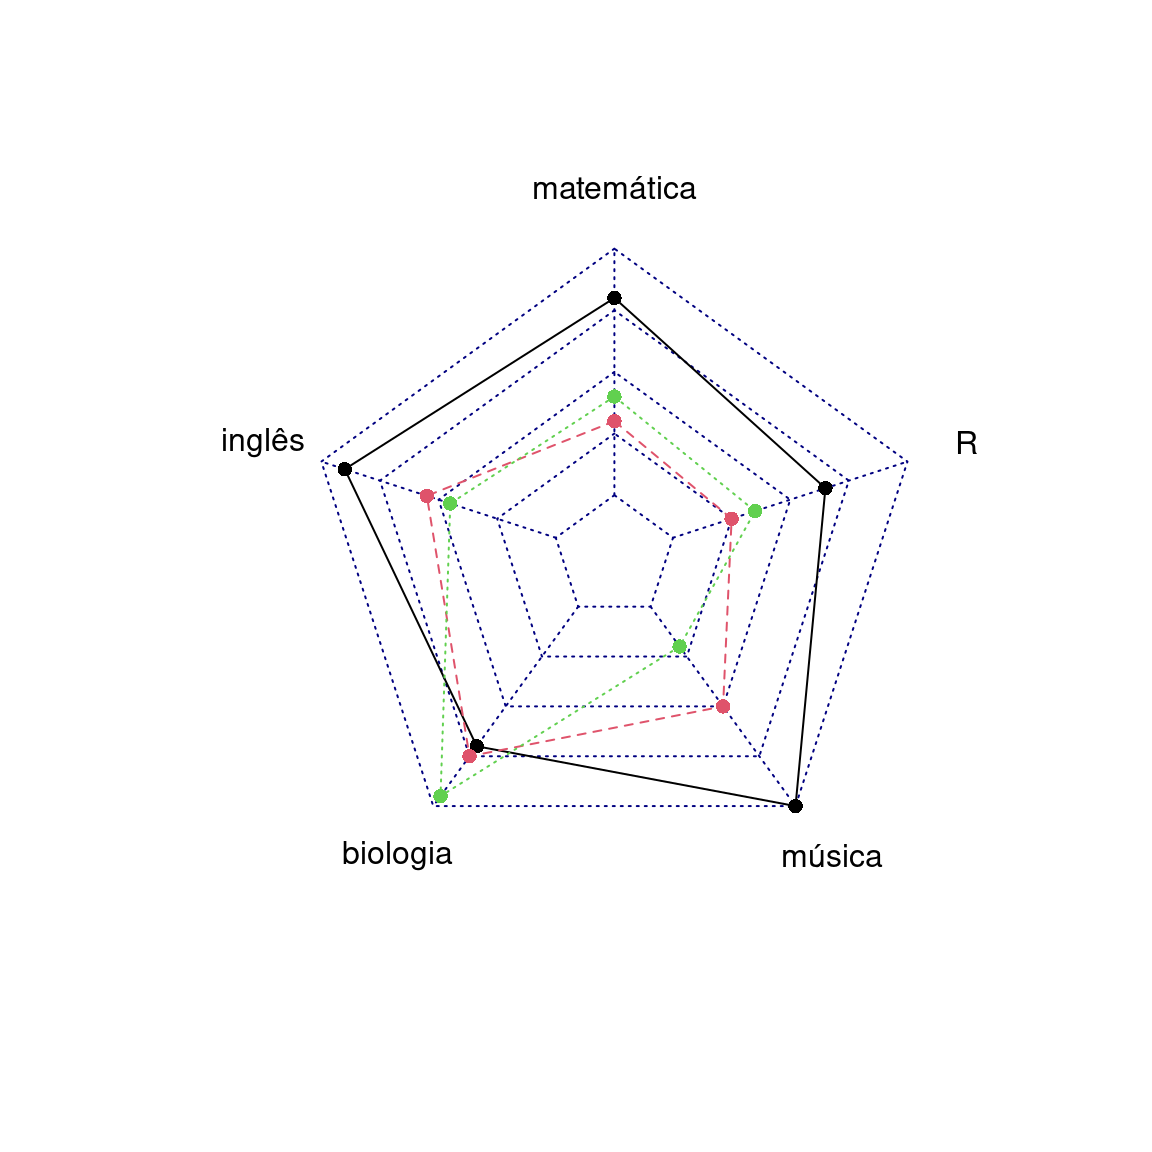
\includegraphics{inferencia_com_R_files/figure-latex/unnamed-chunk-45-1} \end{center}

\hypertarget{conceitos-buxe1sicos}{%
\chapter{Conceitos Básicos}\label{conceitos-buxe1sicos}}

No estudo da inferência estatística, o objetivo principal é obter informações sobre uma população a partir das informações de uma amostra e aqui vamos precisar de definições mais formais de população e amostra. Para facilitar a compreensão destes conceitos, apresentamos o exemplo abaixo a título de ilustração

Em um estudo antropométrico em nível nacional, uma amostra de 5000 adultos é selecionada dentre os adultos brasileiros e uma das variáveis de estudo é a altura.

Neste exemplo, a população é o conjunto de todos os brasileiros adultos. No entanto, o interesse (um deles, pelo menos) está na altura dos brasileiros. Assim, nesse estudo, a cada sujeito da população associamos um número correspondente a sua altura. Se determinado sujeito é sorteado para entrar na amostra, o que nos interessa é esse número, ou seja, sua altura.

Como sabemos, essa é a definição de variável aleatória: uma função que associa a cada ponto do espaço amostral um número real. Dessa forma, a nossa população pode ser representada pela variável aleatória \(X\) = ``altura do adulto brasileiro''. Como essa é uma v.a. contínua, a ela está associada uma função de densidade de probabilidade \(f\) e da literatura, sabemos que é razoável supor que essa densidade seja a densidade normal. Assim, nossa população, nesse caso, é representada por uma v.a. \(X\sim N(\mu; \sigma^2)\). Conhecendo os valores de \(\mu\) e \(\sigma\) teremos informações completas sobre a nossa população.

Uma forma de obtermos os valores de \(\mu\) e \(\sigma\) é medindo as alturas de todos os brasileiros adultos. Mas esse seria um procedimento caro e demorado. Uma solução, então, é retirar uma amostra (subonjunto) da população e estudar essa amostra. Suponhamos que essa amostra seja retirada com reposição e que os sorteios sejam feitos de forma independente, isto é, o resultado de cada extração não altera o resultado das demais extrações. Ao sortearmos o primeiro elemento, estamos realizando um experimento que dá origem a v.a. \(X_1=\) altura do primeiro elemento; o segundo elemento dá origem a v.a. \(X_2=\) ``altura do segundo elemento'' e assim por diante. Como as extrações são feitas com reposição, todas as v.a. \(X_1, X_2, \ldots\) têm a mesma distribuição, que reflete a distribuição da altura de todos os brasileiros adultos. Para uma amostra específica, temos os valores observados \(x_1, x_2, \ldots\) dessas variáveis aleatórias.

\hypertarget{populauxe7uxe3o}{%
\section{População}\label{populauxe7uxe3o}}

A inferência estatística trata do problema de se obter informação sobre uma população a partir de uma amostra. Embora a população real possa ser constituída de pessoas, empresas, animais etc., as pesquisas estatísticas buscam informações sobre determinadas características dos sujeitos, características essas que podem ser representadas por números. Sendo assim, a cada sujeito da população está associado um número, o que nos permite apresentar a seguinte definição.

\textbf{População:} \emph{A população de uma pesquisa estatística pode ser representada por uma variável aleatória $X$ que descreve a característica de interesse.}

Os métodos de inferência nos permitirão obter estimativas dos parâmetros (característica de interesse) de tal variável aleatória, que pode ser contínua ou discreta.

\hypertarget{amostra}{%
\section{Amostra}\label{amostra}}

Embora existam vários métodos de seleção de amostras, nosso foco é a amostragem aleatória simples. Segundo tal método, toda amostra de mesmo tamanho \(n\) tem igual chance (probabilidade) de ser sorteada. É possível extrair amostras aleatórias simples com e sem reposição. No entanto, para populações grandes - ou infinitas - extrações com e sem reposição não levam a resultados muito diferentes. Assim, no estudo da Inferência Estatística, estaremos lidando sempre com amostragem aleatória simples com reposição. Este método de seleção atribui a cada elemento da população a mesma probabilidade de ser selecionado e esta probabilidade se mantém constante ao longo do processo de seleção da amostra (se as extrações fossem sem reposição isso não aconteceria). No restante desse curso omitiremos a expressão ``com reposição'', ou seja, o termo amostragem (ou amostra) aleatória simples sempre se referirá a amostragem com reposição. Por simplicidade, muitas vezes abreviaremos o termo amostra aleatória simples por aas.

Uma forma de se obter uma amostra aleatória simples é escrever os números ou nomes dos elementos da população em cartões iguais, colocar estes cartões em uma urna misturando-os bem e fazer os sorteios necessários, tendo o cuidado de colocar cada cartão sorteado na urna antes do próximo sorteio. Na prática, em geral são usados programas de computador, uma vez que as populações tendem a ser muito grandes.

Agora vamos formalizar o processo de seleção de uma amostra aleatória simples, de forma a relacioná-lo com os problemas de inferência estatística que iremos estudar. Seja uma população representada por uma variável aleatória \(X\). De tal população será sorteada uma amostra aleatória simples com reposição de tamanho \(n\). Como visto nos exemplos anteriores, cada sorteio dá origem a uma variável aleatória \(X_i\) e, como os sorteios são com reposição, todas essas variáveis têm a mesma distribuição de \(X\). Isso nos leva a seguinte definição.

\textbf{Amostra:} \emph{Uma amostra aleatória simples (aas) de tamanho $n$ de uma v.a. $X$ (população) é um conjunto de $n$ v.a. $X_1, X_2, \ldots, X_n$ independentes e identicamente
distribuídas (i.i.d.).}

É interessante notar a convenção usual: o valor observado de uma v.a. \(X\) é representado pela letra minúscula correspondente. Assim, depois do sorteio de uma aas de tamanho \(n\), temos valores observados \(x_1, x_2, \ldots, x_n\) das respectivas variáveis aleatórias.

\hypertarget{estatuxedsticas-e-paruxe2metros}{%
\section{Estatísticas e Parâmetros}\label{estatuxedsticas-e-paruxe2metros}}

Obtida uma aas, é possível calcular diversas características desta amostra, como, por exemplo, a média, a mediana, a variância, etc. Qualquer uma destas características é uma função de \(X_1, X_2, \ldots, X_n\) e, portanto, o seu valor depende da amostra sorteada. Sendo assim, cada uma dessas características ou funções é também uma v.a.. Por exemplo, a média amostral é a v.a. definida por \[\bar X = \frac{X_1+X_2+\ldots+X_n}{n}.\]

Temos, então, a seguinte definição:

\textbf{Estatística:} \emph{Uma estatística amostral ou estimador $T$ é qualquer função da
amostra $X_1, X_2, \ldots, X_n$, isto é, $T = g(X_1, X_2, \ldots, X_n)$ onde $g$ é uma função qualquer.}

As estatísticas amostrais que estaremos considerando neste curso são:

\begin{itemize}
\tightlist
\item
  média amostral: \(\bar X = \frac{1}{n}\sum_{i=1}^n X_i\)
\item
  variância amostral: \(S^2=\frac{1}{n-1}\sum_{i=1}^n (X_i-\bar X)^2\)
\end{itemize}

Para uma amostra específica, o valor obido para o estimador será denominado estimativa e, em geral, serão representadas por letras minúsculas. Por exemplo, temos as seguintes notações correspondentes a média amostral e a variância: \(\bar x\) e \(s^2\).

Outras estatísticas possíveis são o mínimo amostral, o máximo amostral, a amplitude amostral, etc.

De forma análoga, temos as características de interesse da população. No entanto, para diferenciar entre as duas situações (população e amostra), atribuimos nomes diferentes.

\textbf{Parâmetro:} \emph{Um parâmetro é uma característica da população.}

Assim, se a população é representada pela v.a. \(X\), alguns parâmetros são a esperança \(E(X)\) e a variância \(V(X)\). Com relação as características mais usuais, vamos usar a seguinte notação:

\begin{longtable}[]{@{}lll@{}}
\toprule
Característica & Parâmetro (população) & Estatística (amostra) \\
\midrule
\endhead
Média & \(\mu\) & \(\bar X\) \\
Variância & \(\sigma^2\) & \(S^2\) \\
Número de elementos & \(N\) & \(n\) \\
\bottomrule
\end{longtable}

\hypertarget{distribuiuxe7uxf5es-amostrais}{%
\section{Distribuições Amostrais}\label{distribuiuxe7uxf5es-amostrais}}

Nos problemas de inferência, estamos interessados em estimar um parâmetro \(\theta\) da população (por exemplo, a média populacional) através de uma aas \(X_1, X_2, \ldots, X_n\). Para isso, usamos uma estatística \(T\) (por exemplo, a média amostral) e, com base no valor obtido para \(T\) a partir de uma particular amostra, iremos tomar as decisões que o problema exige. Já foi dito que \(T\) é uma v.a., uma vez que depende da amostra sorteada; amostras diferentes fornecerão diferentes valores para \(T\).

Consideremos o seguinte exemplo, onde nossa população é o conjunto \(\{1,3,6,8\}\), isto é, este é o conjunto dos valores da característica de interesse da população em estudo. Assim, para esta população, ou seja, para essa v.a. \(X\) temos \(E(X)=\) 4.5 e \(V(X)=\) 7.25.

Suponha que dessa população iremos extrair uma aas de tamanho 2 e a estatística que iremos calcular é a média amostral. Algumas possibilidades de amostra são \(\{1,1\}\), \(\{1,3\}\), \(\{6,8\}\), para as quais os valores da média amostral são \(1\), \(2\) e \(7\), respectivamente. Podemos ver, então, que há uma variabilidade nos valores da estatística e, assim, seria interessante que conhecêssemos tal variabilidade. Conhecendo tal variabilidade, temos condições de saber ``quão infelizes'' podemos ser no sorteio da amostra. No exemplo acima, as amostras \(\{1,1\}\) e \(\{8,8\}\) são as que têm média amostral mais afastada da verdadeira média populacional. Se esses valores tiverem chance muito mais alta do que os valores mais próximos de \(E(X)\), podemos ter sérios problemas.

Para conhecer o comportamento (distribuição) da média amostral, teríamos que conhecer todos os possíveis valores de \(X\), o que equivaleria a conhecer todas as possíveis amostras de tamanho 2 de tal população. Nesse exemplo, como só temos 4 elementos na população, a obtenção de todas as aas de tamanho 2 não é difícil. No entanto, para um número um pouco maior dele elementos, ou quando não conhecemos todo o espaço amostral, essa tarefa se torna complexa.

\textbf{Distribuição de Probabilidade:}\emph{A função de distribuição amostral de uma estatística $T$ é a função de distribuição de probabilidades de $T$ ao longo de todas as possíveis amostras de tamanho $n$.}

Em outras palavras, uma distribuição amostral é a distribuição de probabilidades de uma medida estatística baseada em uma amostra aleatória. Ao retirar uma amostra aleatória de uma população estaremos considerando cada valor da amostra como um valor de uma variável aleatória cuja distribuição de probabilidade é a mesma da população no instante da retirada desse elemento para a amostra. Em consequência do fato de os valores de amostra serem aleatórios, decorre que qualquer quantidade calculada em função dos elementos da amostra também será uma variável aleatória.

Podemos ver que a obtenção da distribuição amostral de qualquer estatística \(T\) é um processo tão ou mais complicado do que trabalhar com a população inteira. Na prática, o que temos é uma única amostra e com esse resultado é que temos que tomar as decisões pertinentes ao problema em estudo. Esta tomada de decisão, no entanto, será facilitada se conhecermos resultados teóricos sobre o comportamento da distribuição amostral.

\hypertarget{propriedades-dos-estimadores}{%
\section{Propriedades dos Estimadores}\label{propriedades-dos-estimadores}}

Vimos anteriormente que, dada uma população, existem muitas e muitas aas de tamanho \(n\) que podem ser sorteadas. Cada uma dessas amostras resulta em um valor diferente da estatística de interesse (\(\bar X\) e \(S^2\), por exemplo). O que esses resultados estão mostrando é como esses diferentes valores se comportam em relação ao verdadeiro (mas desconhecido) valor do parâmetro.

Considere a Figura abaixo, onde o alvo representa o valor do parâmetro e os ``tiros'', indicados pelos símbolo x, representam os diferentes valores amostrais da estatística de interesse.

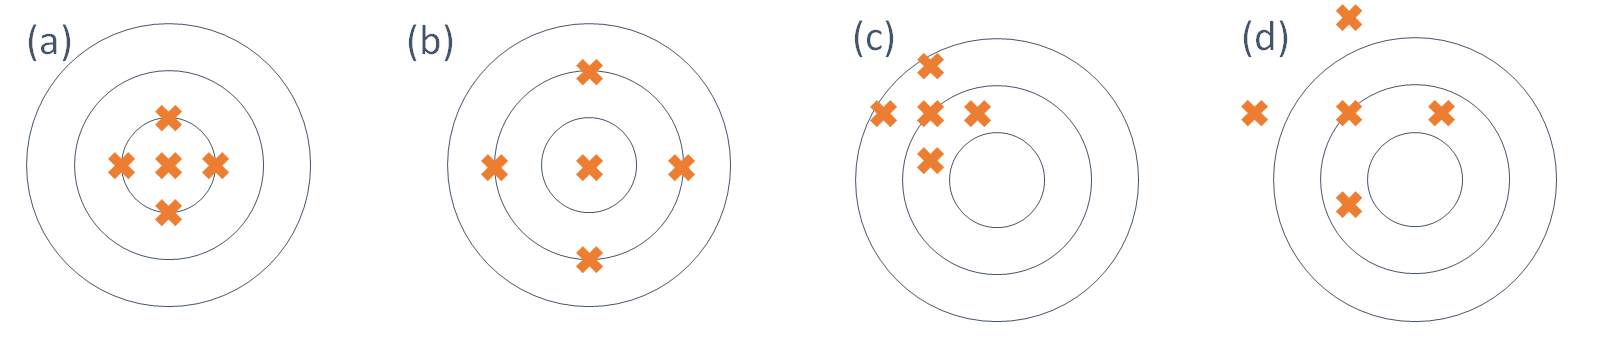
\includegraphics{Estimadores_exemplo.png}

Nas partes (a) e (b) da figura, os tiros estão em torno do alvo, enquanto nas partes (c) e (d) isso não acontece. Comparando as partes (a) e (b), podemos ver que na parte (a) os tiros estão mais concentrados em torno do alvo, isto é, têm menor dispersão. Isso reflete uma pontaria mais certeira do atirador em (a). Analogamente, nas partes (c) e (d), embora ambos os atiradores estejam com a mira deslocada, os tiros do atirador (c) estão mais concentrados em torno de um alvo; o deslocamento poderia até ser resultado de um desalinhamento da arma. Já o atirador (d), além de estar com o alvo deslocado, ele tem os tiros mais espalhados, o que reflete menor precisão.

Traduzindo esta situação para o contexto de estimadores e suas propriedades, temos o seguinte: nas partes (a) e (b), temos dois estimadores que fornecem estimativas centradas em torno do verdadeiro valor do parâmetro, ou seja, as diferentes amostras fornecem valores distribuídos em torno do verdadeiro valor do parâmetro. A diferença é que em (b) esses valores estão mais dispersos e, assim, temos mais chance de obter uma amostra ``infeliz'', ou seja, uma amostra que forneça um resultado muito afastado do valor do parâmetro. Essas duas propriedades estão associadas a esperança e a variância do estimador, que são medidas de centro e dispersão, respectivamente. Nas partes (c) e (d), as estimativas estão centradas em torno de um valor diferente do parâmetro de interesse e na parte (d), a dispersão é maior.

Temos, assim, ilustrados os seguintes conceitos:

\textbf{Viés:}\emph{Um estimador $T$ é dito um estimador não-viesado do parâmetro $\theta$ se $E(T)=\theta$.}

Essa esperança é calculada ao longo de todas as possíveis amostras, ou seja, é a esperança da distribuição amostral de \(T\). Nas partes (a) e (b) da Figura os estimadores são não-viesados e nas partes (c) e (d), os estimadores são viesados.

Com relação aos estimadores \(bar X\), \(S^2\) e \(\hat \sigma^2\), veremos formalmente que os dois primeiros são não-viesados para estimar a média e a variância populacionais, respectivamente, enquanto \(\hat \sigma^2\) é viesado para estimar a variância populacional. Essa é a razão para se usar \(S^2\), e não \(\hat \sigma^2\).

\textbf{Eficiência:}\emph{Se $T_1$ e $T_2$ são dois estimadores não-viesados do parâmetro $\theta$, diz-se que $T_1$ é mais eficiente que $T_2$ se $V(T_1)<V(T_2)$.}

Na Figura, o estimador da parte (a) é mais eficiente que o estimador da parte (b). Uma outra propriedade dos estimadores está relacionada a idéia bastante intuitiva de que a medida que se aumenta o tamanho da amostra, mais perto devemos ficar do verdadeiro valor do parâmetro.

\textbf{Consistência:}\emph{Um estimador $T$ de um parâmetro $\theta$ é consistente se:}

\begin{itemize}
\tightlist
\item
  \(\lim_{n\to\infty} E(\hat\theta)=\theta\)
\item
  \(\lim_{n\to\infty} V(\hat\theta)=0\)
\end{itemize}

\hypertarget{distribuiuxe7uxf5es-amostrais-1}{%
\chapter{Distribuições Amostrais}\label{distribuiuxe7uxf5es-amostrais-1}}

Uma distribuição amostral é a distribuição de probabilidades de uma medida estatística baseada em uma amostra aleatória. Ao retirar uma amostra aleatória de uma população estaremos considerando cada valor da amostra como um valor de uma variável aleatória cuja distribuição de probabilidade é a mesma da população no instante da retirada desse elemento para a amostra. Em consequência do fato de os valores de amostra serem aleatórios, decorre que qualquer quantidade calculada em função dos elementos da amostra também será uma variável aleatória

\hypertarget{distribuiuxe7uxe3o-da-muxe9dia-amostral}{%
\section{Distribuição da Média Amostral}\label{distribuiuxe7uxe3o-da-muxe9dia-amostral}}

Considere \(X_1,\ldots,X_n\) uma amostra aleatória de uma distribuição normal com média \(\mu\) e variância \(\sigma^2\).

Tomamos, por exemplo, o problema de estimar quantas horas adicionais de sono são garantidas a um indivíduo após ingerir uma determinada droga. Além disso, suponha que a droga é testada em 20 indivíduos de modo que a média amostral seja \(\bar X=0,8\) horas. Porém, se o estudo for repetido com outros 20 participantes podemos ter outros resultados para a média amostral. Por exemplo, podemos ter \(\bar X=1,3\). E, repetindo o estudo novamente, poderíamos ter \(\bar X=-0,2\). Em termos estatísticos, haverá variação entre as médias amostrais.

Este problema poderia ser resolvido se repetíssemos o estudo infinitas vezes, porém isto é inviável.

Quando as observações são amostradas aleatoriamente de uma distribuição normal, a média amostral também tem uma distribuição normal. Isto é, quando \(n\) observações são amostradas aleatoriamente de uma distribuição normal com média \(\mu\) e variância \(\sigma^2\), a média amostral tem distribuição normal com média \(\mu\) e variância \(\frac{\sigma^2}{n}\). Ou seja, se

\[X\sim N(\mu,\sigma^2)\text{, então} \bar X \sim N\left(\mu,\frac{\sigma^2}{n}\right).\]

\hypertarget{visualizando}{%
\subsection{Visualizando}\label{visualizando}}

Considere uma população normal com média \(\mu=10\) e variância \(\sigma^2=4\). Vamos realizar um estudo de simulação para a distribuição da média amostral considerando amostras de tamanho 20 dessa população.

Primeiramente, considere que são retiradas 15 amostras de tamanho 20 dessa população.

\begin{Shaded}
\begin{Highlighting}[]
\FunctionTok{library}\NormalTok{(ggplot2)}
\NormalTok{n }\OtherTok{=} \DecValTok{15}
\NormalTok{matriz\_aux }\OtherTok{=} \FunctionTok{matrix}\NormalTok{(}\ConstantTok{NA}\NormalTok{,}\AttributeTok{nrow=}\DecValTok{20}\NormalTok{,}\AttributeTok{ncol=}\NormalTok{n)}
\ControlFlowTok{for}\NormalTok{(j }\ControlFlowTok{in} \DecValTok{1}\SpecialCharTok{:}\FunctionTok{ncol}\NormalTok{(matriz\_aux))\{matriz\_aux[,j]}\OtherTok{=}\FunctionTok{rnorm}\NormalTok{(}\DecValTok{20}\NormalTok{,}\AttributeTok{mean=}\DecValTok{10}\NormalTok{,}\AttributeTok{sd=}\DecValTok{2}\NormalTok{)\}}
\NormalTok{medias }\OtherTok{=} \FunctionTok{data.frame}\NormalTok{(}\AttributeTok{x=}\DecValTok{1}\SpecialCharTok{:}\FunctionTok{ncol}\NormalTok{(matriz\_aux),}\AttributeTok{y=}\FunctionTok{colMeans}\NormalTok{(matriz\_aux))}
\FunctionTok{ggplot}\NormalTok{(medias,}\FunctionTok{aes}\NormalTok{(y)) }\SpecialCharTok{+}
  \FunctionTok{geom\_histogram}\NormalTok{(}\AttributeTok{color =} \StringTok{"white"}\NormalTok{) }\SpecialCharTok{+}
  \FunctionTok{theme}\NormalTok{(}\AttributeTok{axis.title =} \FunctionTok{element\_blank}\NormalTok{())}
\end{Highlighting}
\end{Shaded}

\begin{center}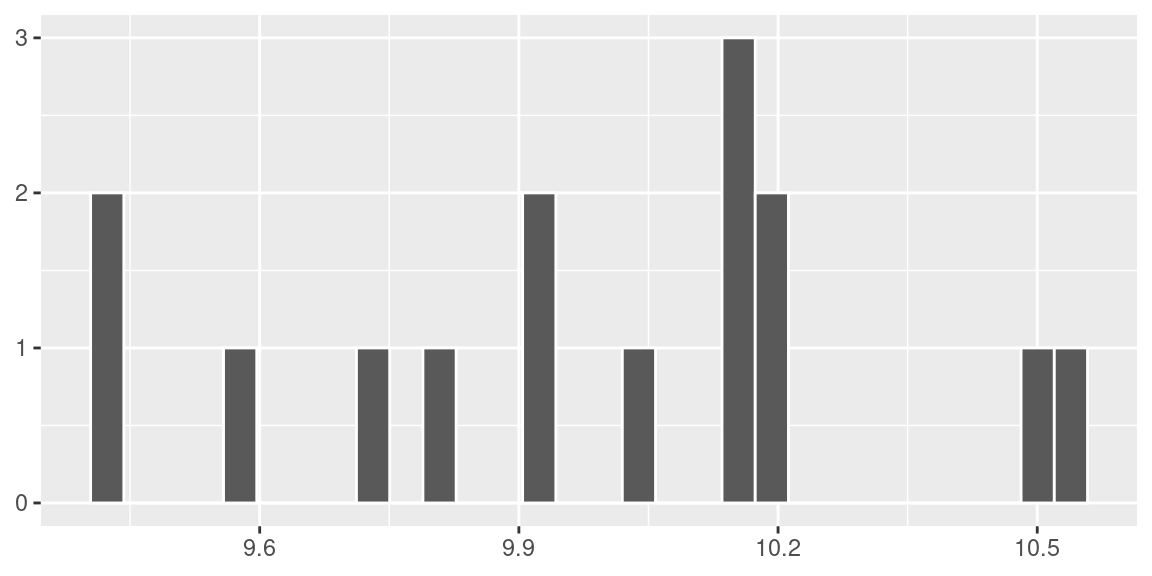
\includegraphics{inferencia_com_R_files/figure-latex/unnamed-chunk-48-1} \end{center}

Nessa simulação obtivemos \(\bar x =\) 10.05 e \(s =\) 0.36.

Suponha agora que façamos o mesmo processo, porém ao invés de considerarmos 15 amostras de tamanho 20, consideramos 200 amostras.

\begin{Shaded}
\begin{Highlighting}[]
\NormalTok{n }\OtherTok{=} \DecValTok{200}
\NormalTok{matriz\_aux }\OtherTok{=} \FunctionTok{matrix}\NormalTok{(}\ConstantTok{NA}\NormalTok{,}\AttributeTok{nrow=}\DecValTok{20}\NormalTok{,}\AttributeTok{ncol=}\NormalTok{n)}
\ControlFlowTok{for}\NormalTok{(j }\ControlFlowTok{in} \DecValTok{1}\SpecialCharTok{:}\FunctionTok{ncol}\NormalTok{(matriz\_aux))\{matriz\_aux[,j]}\OtherTok{=}\FunctionTok{rnorm}\NormalTok{(}\DecValTok{20}\NormalTok{,}\AttributeTok{mean=}\DecValTok{10}\NormalTok{,}\AttributeTok{sd=}\DecValTok{2}\NormalTok{)\}}
\NormalTok{medias }\OtherTok{=} \FunctionTok{data.frame}\NormalTok{(}\AttributeTok{x=}\DecValTok{1}\SpecialCharTok{:}\FunctionTok{ncol}\NormalTok{(matriz\_aux),}\AttributeTok{y=}\FunctionTok{colMeans}\NormalTok{(matriz\_aux))}
\FunctionTok{ggplot}\NormalTok{(medias,}\FunctionTok{aes}\NormalTok{(y)) }\SpecialCharTok{+}
  \FunctionTok{geom\_histogram}\NormalTok{(}\AttributeTok{color =} \StringTok{"white"}\NormalTok{) }\SpecialCharTok{+}
  \FunctionTok{theme}\NormalTok{(}\AttributeTok{axis.title =} \FunctionTok{element\_blank}\NormalTok{())}
\end{Highlighting}
\end{Shaded}

\begin{center}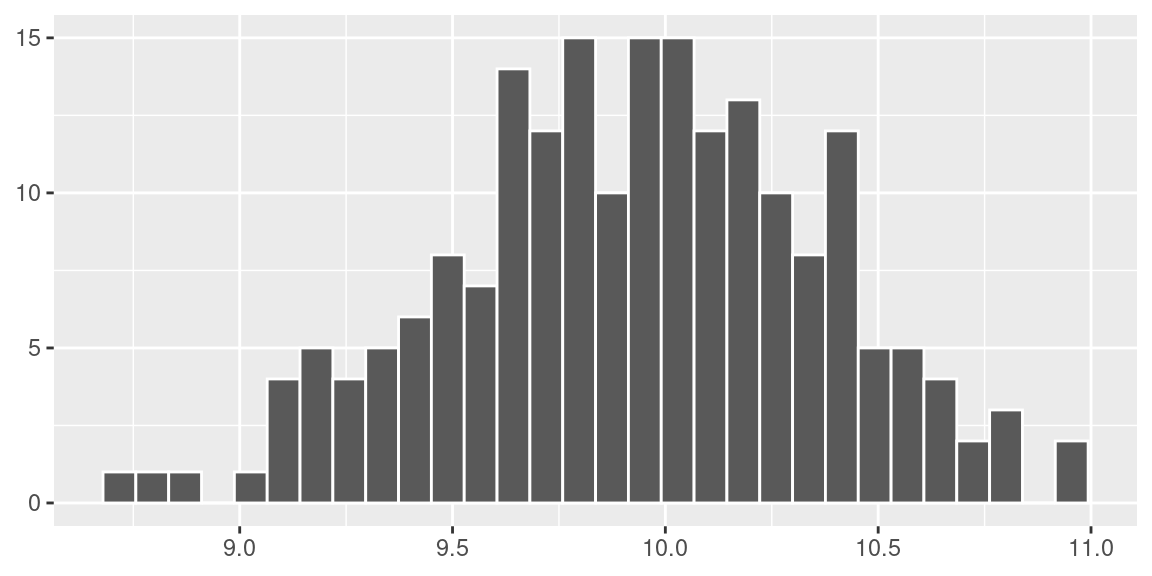
\includegraphics{inferencia_com_R_files/figure-latex/unnamed-chunk-49-1} \end{center}

Agora, obtivemos \(\bar x =\) 10 e \(s =\) 0.45.

Realizando o mesmo experimento, porém agora considerando 10000 amostras de tamanho 20, a distribuição da média amostral pode ser vista segundo o histograma abaixo.

\begin{Shaded}
\begin{Highlighting}[]
\NormalTok{n }\OtherTok{=} \DecValTok{10000}
\NormalTok{matriz\_aux }\OtherTok{=} \FunctionTok{matrix}\NormalTok{(}\ConstantTok{NA}\NormalTok{,}\AttributeTok{nrow=}\DecValTok{20}\NormalTok{,}\AttributeTok{ncol=}\NormalTok{n)}
\ControlFlowTok{for}\NormalTok{(j }\ControlFlowTok{in} \DecValTok{1}\SpecialCharTok{:}\FunctionTok{ncol}\NormalTok{(matriz\_aux))\{matriz\_aux[,j]}\OtherTok{=}\FunctionTok{rnorm}\NormalTok{(}\DecValTok{20}\NormalTok{,}\AttributeTok{mean=}\DecValTok{10}\NormalTok{,}\AttributeTok{sd=}\DecValTok{2}\NormalTok{)\}}
\NormalTok{medias }\OtherTok{=} \FunctionTok{data.frame}\NormalTok{(}\AttributeTok{x=}\DecValTok{1}\SpecialCharTok{:}\FunctionTok{ncol}\NormalTok{(matriz\_aux),}\AttributeTok{y=}\FunctionTok{colMeans}\NormalTok{(matriz\_aux))}
\FunctionTok{ggplot}\NormalTok{(medias,}\FunctionTok{aes}\NormalTok{(y)) }\SpecialCharTok{+}
  \FunctionTok{geom\_histogram}\NormalTok{(}\AttributeTok{color =} \StringTok{"white"}\NormalTok{) }\SpecialCharTok{+}
  \FunctionTok{theme}\NormalTok{(}\AttributeTok{axis.title =} \FunctionTok{element\_blank}\NormalTok{())}
\end{Highlighting}
\end{Shaded}

\begin{center}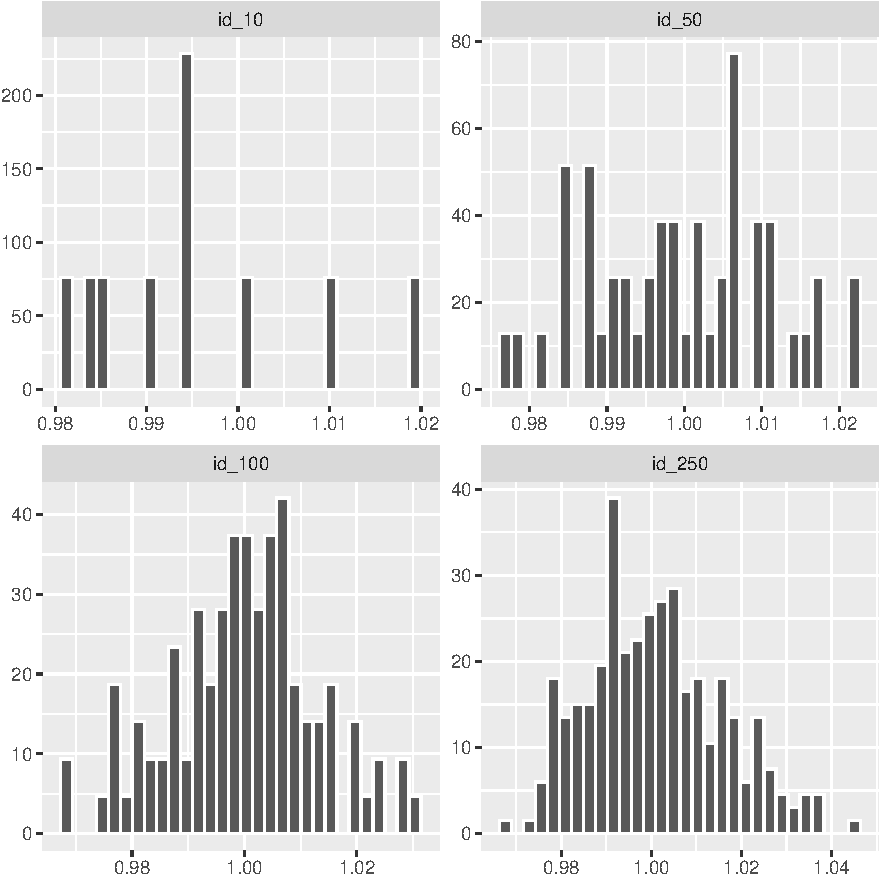
\includegraphics{inferencia_com_R_files/figure-latex/unnamed-chunk-50-1} \end{center}

Para este caso, a média das médias amostrais foi \(\bar x=\) 10 e o desvio padrão foi \(s =\) 0.45. Então, empiricamente, podemos perceber que a distribuição da média amostral se aproxima de uma distribuição normal com média \(\mu=10\) e desvio padrão \(\frac{\sigma}{\sqrt{n}}=\frac{2}{\sqrt{20}}=0,4472\).

\hypertarget{prova}{%
\subsection{Prova}\label{prova}}

Para provar que se \(X\sim N(\mu,\sigma^2)\), então \(\bar X \sim N(\mu,\frac{\sigma^2}{n})\), vamos precisar de somente três passos.

\begin{enumerate}
\def\labelenumi{\arabic{enumi}.}
\tightlist
\item
  Dado que \(\bar X = \frac{1}{n}\sum_{i=1}^{n}X_i\), onde \(X_1,\ldots,X_n\) é uma amostra aleatória de tamanho \(n\) de uma população Normal sabemos que combinação linear de Normais resulta em também uma distribuição Normal, portanto daqui temos que \(\bar X \sim Normal\);
\item
  Se \(\bar X = \frac{1}{n}\sum_{i=1}^{n}X_i\), então \[E\left[\bar X\right] = E\left[\frac{1}{n}\sum_{i=1}^{n}X_i\right]=\frac{1}{n}\sum_{i=1}^{n}E\left[X_i\right]=\frac{n\mu}{n}=\mu\]
\item
  Por fim, se \(\bar X = \frac{1}{n}\sum_{i=1}^{n}X_i\), então como os \(X_i\)'s são independentes \[V \left[\bar X\right] = V\left[\frac{1}{n}\sum_{i=1}^{n}X_i\right]=\frac{1}{n^2}\sum_{i=1}^{n}V\left[X_i\right]=\frac{n\sigma^2}{n^2}=\frac{\sigma^2}{n}\]
\end{enumerate}

\hypertarget{teorema-central-do-limite}{%
\section{Teorema Central do Limite}\label{teorema-central-do-limite}}

Os resultados vistos anteriormente são válidos para populações normais, isto é, se uma população é normal com média \(\mu\) e variância \(\sigma^2\), então a distribuição amostral de \(\bar X\) é também normal com média \(\mu\) e variância \(\frac{\sigma^2}{n}\), onde \(n\) é o tamanho da amostra. O Teorema Central do Limite (TCL) nos fornece um resultado análogo para qualquer distribuição populacional, desde que o tamanho da amostra seja suficientemente grande.

Seja \(X_1,\ldots,X_n\) uma amostra aleatória simples de uma população \(X\) tal que \(E(X)=\mu\) e \(V(X)=\sigma^2\). Então, a distribuição de \(\bar X\) converge para a distribuição Normal com média \(\mu\) e variância \(\frac{\sigma^2}{n}\) quando \(n\rightarrow \infty\). Equivalentemente, \[\frac{\bar X-\mu}{\frac{\sigma}{\sqrt{n}}}\rightarrow N(0,1)\]

A interpretação prática do TCL é a seguinte: para amostras ``grandes'' de qualquer população, podemos aproximar a distribuição amostral de \(\bar X\) por uma distribuição normal com a mesma média populacional e variância igual à variância populacional dividida pelo tamanho da amostra.

Quão grande deve ser a amostra para se obter uma boa aproximação depende das características da distribuição populacional. Se a distribuição populacional não se afastar muito de uma distribuição normal, a aproximação será boa, mesmo para tamanhos pequenos de amostra. Em termos práticos, esse teorema é de extrema importância, daí ser chamado de Teorema Central e, em geral, amostras de tamanho \(n>30\) já fornecem uma aproximação razoável.

\hypertarget{visualizando-1}{%
\subsection{Visualizando}\label{visualizando-1}}

Considere uma população exponencial com média \(\mu=1\), ou seja, uma população distribuída segundo uma exponencial com parâmetro \(\lambda=1\).

O gráfico superior representa a distribuição populacional e os histogramas representam a distribuição amostral de \(\bar X\) ao longo de 5000 amostras de tamanhos 10, 50, 100 e 250. Assim, podemos ver que, embora a população seja completamente diferente da normal, a distribuição amostral de \(\bar X\) vai se tornando cada vez mais próxima da normal à medida que \(n\) aumenta.

\begin{Shaded}
\begin{Highlighting}[]
\NormalTok{matriz\_aux\_10 }\OtherTok{=} \FunctionTok{matrix}\NormalTok{(}\ConstantTok{NA}\NormalTok{,}\AttributeTok{nrow=}\DecValTok{5000}\NormalTok{,}\AttributeTok{ncol=}\DecValTok{10}\NormalTok{)}
\NormalTok{matriz\_aux\_50 }\OtherTok{=} \FunctionTok{matrix}\NormalTok{(}\ConstantTok{NA}\NormalTok{,}\AttributeTok{nrow=}\DecValTok{5000}\NormalTok{,}\AttributeTok{ncol=}\DecValTok{50}\NormalTok{)}
\NormalTok{matriz\_aux\_100 }\OtherTok{=} \FunctionTok{matrix}\NormalTok{(}\ConstantTok{NA}\NormalTok{,}\AttributeTok{nrow=}\DecValTok{5000}\NormalTok{,}\AttributeTok{ncol=}\DecValTok{100}\NormalTok{)}
\NormalTok{matriz\_aux\_250 }\OtherTok{=} \FunctionTok{matrix}\NormalTok{(}\ConstantTok{NA}\NormalTok{,}\AttributeTok{nrow=}\DecValTok{5000}\NormalTok{,}\AttributeTok{ncol=}\DecValTok{250}\NormalTok{)}
\ControlFlowTok{for}\NormalTok{(j }\ControlFlowTok{in} \DecValTok{1}\SpecialCharTok{:}\FunctionTok{ncol}\NormalTok{(matriz\_aux\_10))\{matriz\_aux\_10[,j]}\OtherTok{=}\FunctionTok{rexp}\NormalTok{(}\DecValTok{5000}\NormalTok{,}\AttributeTok{rate=}\DecValTok{1}\NormalTok{)\}}
\ControlFlowTok{for}\NormalTok{(j }\ControlFlowTok{in} \DecValTok{1}\SpecialCharTok{:}\FunctionTok{ncol}\NormalTok{(matriz\_aux\_50))\{matriz\_aux\_50[,j]}\OtherTok{=}\FunctionTok{rexp}\NormalTok{(}\DecValTok{5000}\NormalTok{,}\AttributeTok{rate=}\DecValTok{1}\NormalTok{)\}}
\ControlFlowTok{for}\NormalTok{(j }\ControlFlowTok{in} \DecValTok{1}\SpecialCharTok{:}\FunctionTok{ncol}\NormalTok{(matriz\_aux\_100))\{matriz\_aux\_100[,j]}\OtherTok{=}\FunctionTok{rexp}\NormalTok{(}\DecValTok{5000}\NormalTok{,}\AttributeTok{rate=}\DecValTok{1}\NormalTok{)\}}
\ControlFlowTok{for}\NormalTok{(j }\ControlFlowTok{in} \DecValTok{1}\SpecialCharTok{:}\FunctionTok{ncol}\NormalTok{(matriz\_aux\_250))\{matriz\_aux\_250[,j]}\OtherTok{=}\FunctionTok{rexp}\NormalTok{(}\DecValTok{5000}\NormalTok{,}\AttributeTok{rate=}\DecValTok{1}\NormalTok{)\}}
\NormalTok{medias\_10 }\OtherTok{=} \FunctionTok{data.frame}\NormalTok{(}\AttributeTok{x=}\DecValTok{1}\SpecialCharTok{:}\FunctionTok{ncol}\NormalTok{(matriz\_aux\_10),}\AttributeTok{y=}\FunctionTok{colMeans}\NormalTok{(matriz\_aux\_10),}\AttributeTok{label=}\StringTok{"id\_10"}\NormalTok{)}
\NormalTok{medias\_50 }\OtherTok{=} \FunctionTok{data.frame}\NormalTok{(}\AttributeTok{x=}\DecValTok{1}\SpecialCharTok{:}\FunctionTok{ncol}\NormalTok{(matriz\_aux\_50),}\AttributeTok{y=}\FunctionTok{colMeans}\NormalTok{(matriz\_aux\_50),}\AttributeTok{label=}\StringTok{"id\_50"}\NormalTok{)}
\NormalTok{medias\_100 }\OtherTok{=} \FunctionTok{data.frame}\NormalTok{(}\AttributeTok{x=}\DecValTok{1}\SpecialCharTok{:}\FunctionTok{ncol}\NormalTok{(matriz\_aux\_100),}\AttributeTok{y=}\FunctionTok{colMeans}\NormalTok{(matriz\_aux\_100),}\AttributeTok{label=}\StringTok{"id\_100"}\NormalTok{)}
\NormalTok{medias\_250 }\OtherTok{=} \FunctionTok{data.frame}\NormalTok{(}\AttributeTok{x=}\DecValTok{1}\SpecialCharTok{:}\FunctionTok{ncol}\NormalTok{(matriz\_aux\_250),}\AttributeTok{y=}\FunctionTok{colMeans}\NormalTok{(matriz\_aux\_250),}\AttributeTok{label=}\StringTok{"id\_250"}\NormalTok{)}
\NormalTok{tudo }\OtherTok{=} \FunctionTok{rbind}\NormalTok{(medias\_10,medias\_50,medias\_100,medias\_250)}
\NormalTok{tudo}\SpecialCharTok{$}\NormalTok{label }\OtherTok{=} \FunctionTok{factor}\NormalTok{(tudo}\SpecialCharTok{$}\NormalTok{label, }\AttributeTok{levels =} \FunctionTok{c}\NormalTok{(}\StringTok{"id\_10"}\NormalTok{, }\StringTok{"id\_50"}\NormalTok{, }\StringTok{"id\_100"}\NormalTok{, }\StringTok{"id\_250"}\NormalTok{))}
\FunctionTok{ggplot}\NormalTok{(tudo,}\FunctionTok{aes}\NormalTok{(y)) }\SpecialCharTok{+}
  \FunctionTok{geom\_histogram}\NormalTok{(}\FunctionTok{aes}\NormalTok{(}\AttributeTok{y=}\NormalTok{..density..),}\AttributeTok{color =} \StringTok{"white"}\NormalTok{) }\SpecialCharTok{+}
  \FunctionTok{facet\_wrap}\NormalTok{(}\SpecialCharTok{\textasciitilde{}}\NormalTok{label, }\AttributeTok{scales =} \StringTok{"free"}\NormalTok{) }\SpecialCharTok{+}
  \FunctionTok{theme}\NormalTok{(}\AttributeTok{axis.title =} \FunctionTok{element\_blank}\NormalTok{())}
\end{Highlighting}
\end{Shaded}

\begin{center}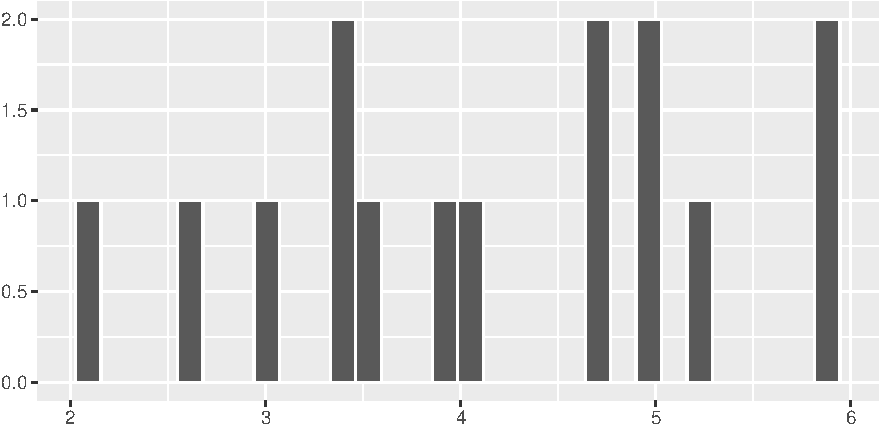
\includegraphics{inferencia_com_R_files/figure-latex/unnamed-chunk-51-1} \end{center}

\hypertarget{distribuiuxe7uxe3o-da-variuxe2ncia-amostral}{%
\section{Distribuição da Variância Amostral}\label{distribuiuxe7uxe3o-da-variuxe2ncia-amostral}}

Já vimos que a estatística \[S^2=\frac{1}{n-1}\sum_{i=1}^{n}\left(X_i-\bar X\right)^2\] é um estimador não viciado da variância \(\sigma^2\), portanto \[E(S^2)=\sigma^2\]. Vamos estudar agora a distribuição amostral de \(S^2\) e para isso precisamos estudar a distribuição qui-quadrado.

\hypertarget{distribuiuxe7uxe3o-qui-quadrado}{%
\subsection{Distribuição Qui-quadrado}\label{distribuiuxe7uxe3o-qui-quadrado}}

Se \(X\) é uma variável aleatória com densidade

\[f_X(x)=\frac{1}{\Gamma\big({\frac{k}{2}}\big)}\big(\frac{1}{2}\big)^{\frac{k}{2}}x^{\frac{k}{2}-1}e^{-\frac{x}{2}},k>0,x>0,\]

onde \(\Gamma(w)=\int_0^\infty x^{w-1}e^{-x}dx, w>0\). Então, \(X\) tem uma distribuição qui-quadrado com \(k\) graus de liberdade, onde o parâmetro \(k\) é um número inteiro.

Para entender a ideia de graus de liberdade, consideremos um conjunto de dados qualquer. Graus de liberdade é o número de valores deste conjunto de dados que podem variar após terem sido impostas certas restrições a todos os valores. Por exemplo, consideremos que 10 estudantes obtiveram em um teste média 8. Assim, a soma das 10 notas deve ser 80 (restrição). Portanto, neste caso, temos um grau de liberdade de \(10-1=9\), pois 9 notas podem variar livremente desde que a soma seja 80, no entanto 1 nota sempre será {[}80-(soma das 9 outras notas){]}.

Temos também que se as variáveis aleatórias \(X_i\), \(i=1,2,\ldots,n\) são independentes e normalmente distribuídas com médias \(\mu_i\) e variâncias \(\sigma^2_i\), isto é \(X_i\sim N(\mu_i,\sigma^2_i)\), então

\[U=\sum_{i=1}^{n}\left(\frac{X_i-\mu}{\sigma^2}\right)^2\]

tem uma distribuição qui-quadrado com \(n\) graus de liberdade.

Além disso, se \(X_1,\ldots,X_n\) é uma a.a. de uma distribuição normal padrão, então, valem as seguintes propriedades:

\begin{enumerate}
\def\labelenumi{(\roman{enumi})}
\item
  \(\bar X\) e \(\sum_{i=1}^{n}(X_i-\bar X)^2\) são independentes;
\item
  \(\sum_{i=1}^{n}(X_i-\bar X)^2\) tem uma distribuição qui-quadrado com \(n-1\) graus de liberdade.
\end{enumerate}

Assim, chegamos que se \(S^2\) é a variância amostral de uma amostra aleatória \(X_1,\ldots,X_n\) de uma distribuição normal com média \(\mu\) e variância \(\sigma^2\), então

\[U=\frac{(n-1)S^2}{\sigma^2}\sim \chi^2_{n-1},\]

ou seja, \(U\) tem uma distribuição qui-quadrado com \(n-1\) graus de liberdade.

\hypertarget{visualizando-2}{%
\subsection{Visualizando}\label{visualizando-2}}

Analogamente ao estudo de simulação realizado no caso da média amostral, considere uma população normal com média \(\mu=10\) e variância \(\sigma^2=4\).

Primeiramente, considere que são retiradas 15 amostras de tamanho 20 dessa população.

\begin{Shaded}
\begin{Highlighting}[]
\NormalTok{n }\OtherTok{=} \DecValTok{15}
\NormalTok{matriz\_aux }\OtherTok{=} \FunctionTok{matrix}\NormalTok{(}\ConstantTok{NA}\NormalTok{,}\AttributeTok{nrow=}\DecValTok{20}\NormalTok{,}\AttributeTok{ncol=}\NormalTok{n)}
\ControlFlowTok{for}\NormalTok{(j }\ControlFlowTok{in} \DecValTok{1}\SpecialCharTok{:}\FunctionTok{ncol}\NormalTok{(matriz\_aux))\{matriz\_aux[,j]}\OtherTok{=}\FunctionTok{rnorm}\NormalTok{(}\DecValTok{20}\NormalTok{,}\AttributeTok{mean=}\DecValTok{10}\NormalTok{,}\AttributeTok{sd=}\DecValTok{2}\NormalTok{)\}}
\NormalTok{variancias }\OtherTok{=} \FunctionTok{data.frame}\NormalTok{(}\AttributeTok{x=}\DecValTok{1}\SpecialCharTok{:}\FunctionTok{ncol}\NormalTok{(matriz\_aux),}\AttributeTok{y=}\FunctionTok{apply}\NormalTok{(matriz\_aux,}\DecValTok{2}\NormalTok{,var))}
\FunctionTok{ggplot}\NormalTok{(variancias,}\FunctionTok{aes}\NormalTok{(y)) }\SpecialCharTok{+}
  \FunctionTok{geom\_histogram}\NormalTok{(}\AttributeTok{color =} \StringTok{"white"}\NormalTok{) }\SpecialCharTok{+}
  \FunctionTok{theme}\NormalTok{(}\AttributeTok{axis.title =} \FunctionTok{element\_blank}\NormalTok{())}
\end{Highlighting}
\end{Shaded}

\begin{center}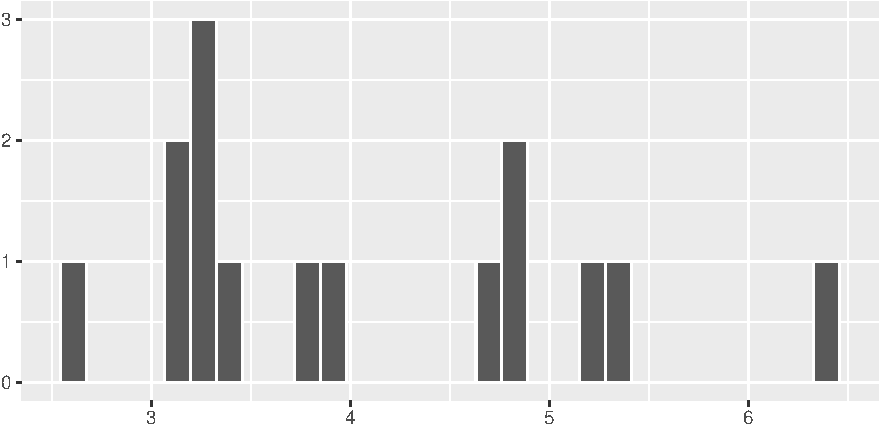
\includegraphics{inferencia_com_R_files/figure-latex/unnamed-chunk-52-1} \end{center}

Nessa simulação obtivemos a média das variâncias igual a 4.07 e a variância das variâncias igual a 1.15.

Suponha agora que façamos o mesmo processo, porém ao invés de considerarmos 15 amostras de tamanho 20, consideramos 1000 amostras.

\begin{Shaded}
\begin{Highlighting}[]
\NormalTok{n }\OtherTok{=} \DecValTok{1000}
\NormalTok{matriz\_aux }\OtherTok{=} \FunctionTok{matrix}\NormalTok{(}\ConstantTok{NA}\NormalTok{,}\AttributeTok{nrow=}\DecValTok{20}\NormalTok{,}\AttributeTok{ncol=}\NormalTok{n)}
\ControlFlowTok{for}\NormalTok{(j }\ControlFlowTok{in} \DecValTok{1}\SpecialCharTok{:}\FunctionTok{ncol}\NormalTok{(matriz\_aux))\{matriz\_aux[,j]}\OtherTok{=}\FunctionTok{rnorm}\NormalTok{(}\DecValTok{20}\NormalTok{,}\AttributeTok{mean=}\DecValTok{10}\NormalTok{,}\AttributeTok{sd=}\DecValTok{2}\NormalTok{)\}}
\NormalTok{variancias }\OtherTok{=} \FunctionTok{data.frame}\NormalTok{(}\AttributeTok{x=}\DecValTok{1}\SpecialCharTok{:}\FunctionTok{ncol}\NormalTok{(matriz\_aux),}\AttributeTok{y=}\FunctionTok{apply}\NormalTok{(matriz\_aux,}\DecValTok{2}\NormalTok{,var))}
\FunctionTok{ggplot}\NormalTok{(variancias,}\FunctionTok{aes}\NormalTok{(y)) }\SpecialCharTok{+}
  \FunctionTok{geom\_histogram}\NormalTok{(}\AttributeTok{color =} \StringTok{"white"}\NormalTok{) }\SpecialCharTok{+}
  \FunctionTok{theme}\NormalTok{(}\AttributeTok{axis.title =} \FunctionTok{element\_blank}\NormalTok{())}
\end{Highlighting}
\end{Shaded}

\begin{center}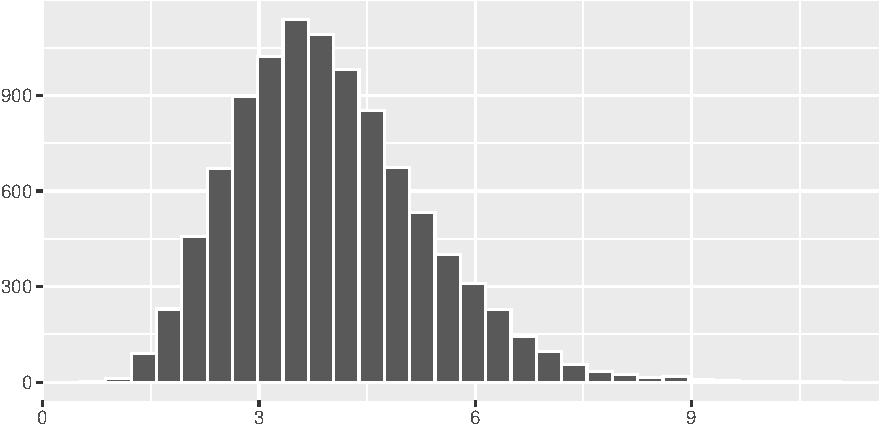
\includegraphics{inferencia_com_R_files/figure-latex/unnamed-chunk-53-1} \end{center}

Neste caso a média das variâncias foi igual a 4.03 e a variância das variâncias igual a 1.72.

Realizando o mesmo experimento, porém agora considerando 10000 amostras de tamanho 20, a distribuição da variância amostral pode ser vista segundo o histograma abaixo.

\begin{Shaded}
\begin{Highlighting}[]
\NormalTok{n }\OtherTok{=} \DecValTok{10000}
\NormalTok{matriz\_aux }\OtherTok{=} \FunctionTok{matrix}\NormalTok{(}\ConstantTok{NA}\NormalTok{,}\AttributeTok{nrow=}\DecValTok{20}\NormalTok{,}\AttributeTok{ncol=}\NormalTok{n)}
\ControlFlowTok{for}\NormalTok{(j }\ControlFlowTok{in} \DecValTok{1}\SpecialCharTok{:}\FunctionTok{ncol}\NormalTok{(matriz\_aux))\{matriz\_aux[,j]}\OtherTok{=}\FunctionTok{rnorm}\NormalTok{(}\DecValTok{20}\NormalTok{,}\AttributeTok{mean=}\DecValTok{10}\NormalTok{,}\AttributeTok{sd=}\DecValTok{2}\NormalTok{)\}}
\NormalTok{variancias }\OtherTok{=} \FunctionTok{data.frame}\NormalTok{(}\AttributeTok{x=}\DecValTok{1}\SpecialCharTok{:}\FunctionTok{ncol}\NormalTok{(matriz\_aux),}\AttributeTok{y=}\FunctionTok{apply}\NormalTok{(matriz\_aux,}\DecValTok{2}\NormalTok{,var))}
\FunctionTok{ggplot}\NormalTok{(variancias,}\FunctionTok{aes}\NormalTok{(y)) }\SpecialCharTok{+}
  \FunctionTok{geom\_histogram}\NormalTok{(}\AttributeTok{color =} \StringTok{"white"}\NormalTok{) }\SpecialCharTok{+}
  \FunctionTok{theme}\NormalTok{(}\AttributeTok{axis.title =} \FunctionTok{element\_blank}\NormalTok{())}
\end{Highlighting}
\end{Shaded}

\begin{center}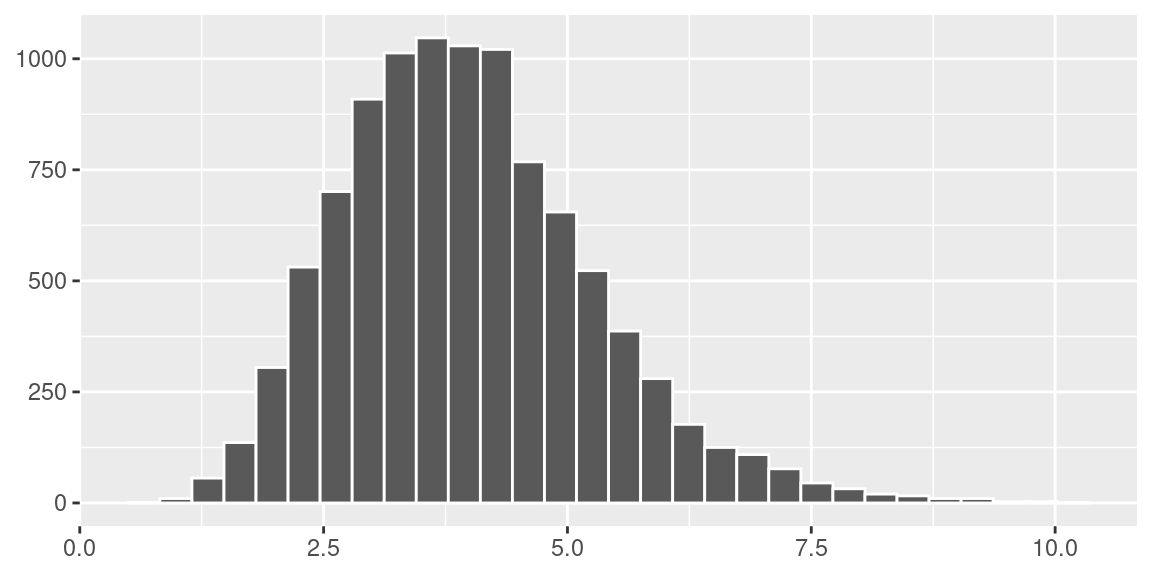
\includegraphics{inferencia_com_R_files/figure-latex/unnamed-chunk-54-1} \end{center}

Neste caso, a média das variâncias é 3.99 e a variância é 1.68. Então, realmente, podemos perceber que a distribuição da variância amostral se aproxima de uma distribuição qui-quadrado com média \(\mu=4\) e variância \(\frac{2\sigma^4}{n-1}=\frac{2\times 16}{19}=1,684\).

Destas propriedades temos que \[V(S^2)=\frac{2\sigma^4}{n-1}.\]

\hypertarget{distribuiuxe7uxe3o-da-proporuxe7uxe3o-amostral}{%
\section{Distribuição da Proporção Amostral}\label{distribuiuxe7uxe3o-da-proporuxe7uxe3o-amostral}}

Considere uma população em que cada elemento é classificado de acordo com a presença ou ausência de determinada característica. Por exemplo, podemos pensar em eleitores escolhendo entre 2 candidatos, pessoas classificadas de acordo com o sexo, trabalhadores classificados como trabalhador com carteira assinada ou não, e assim por diante. Em termos de variável aleatória, essa população é representada por uma v.a. de Bernoulli, isto é:

\[
X=\begin{cases}
1,~\text{se elemento possui a característica de interesse}\\
0,~\text{se elemento não possui a caracaterística de interesse}
\end{cases}
\]

Vamos denotar por \(p\) a proporção de elementos da população que possuem a característica de interesse. Então, \(P(X = 1) = p\), \(E(X) = p\) e \(V(X) = p(1 -p)\). Em geral, esse parâmetro é desconhecido e precisamos estimá-lo a partir de uma amostra.

Suponha, então, que dessa população seja extraída uma amostra aleatória simples \(X_1, X_2, \ldots , X_n\) com reposição. Essas \(n\) extrações correspondem a \(n\) variáveis aleatórias de Bernoulli independentes e, como sabemos, \(S_n =\sum_{i=1}^n X_i\) tem distribuição binomial com parâmetros \(n\) e \(p\).

Note que \(S_n\) dá o número total de ``sucessos'' nas \(n\) repetições, onde ``sucesso'', neste caso, representa a presença da característica de interesse. Os valores possíveis de \(S_n\) são \(0, 1, 2,\ldots , n\). Com relação à proporção \(\hat P\) de elementos na amostra que possuem a característica de interesse, temos que

\[\hat P = \frac{S_n}{n}=\frac{X_1+X_2+\ldots+X_n}{n}\]

e os valores possíveis de \(\hat P\) são \(0,\frac{1}{n},\frac{2}{n},\ldots,\frac{n-1}{n},1\) com

\[P\left(\hat P = \frac{k}{n}\right)=P(S_n=k).\]
Como a proporção amostral é uma média de uma amostra aleatória simples de uma população com distribuição de Bernoulli com parâmetro \(p\), o Teorema Limite Central nos diz, então, que a distribuição da proporção amostral se aproxima de uma normal com média \(p\) e variância \(\frac{p(1-p)}{n}\). Isto é,

\[\hat p \sim N\left(p,\frac{p(1-p)}{n}\right).\]

Como essa aproximação é uma conseqüência direta da aproximação normal da binomial, as mesmas regras continuam valendo: a aproximação deve ser feita se \(np \geq 5\) e \(n(1 - p) \geq 5\).

\hypertarget{visualizando-3}{%
\subsection{Visualizando}\label{visualizando-3}}

Considere uma população bernoulli com \(p=0,3\). Vamos realizar um estudo de simulação para a distribuição da proporção amostral considerando amostras de tamanho 20 dessa população.

Primeiramente, considere que são retiradas 15 amostras de tamanho 20 dessa população.

\begin{Shaded}
\begin{Highlighting}[]
\FunctionTok{library}\NormalTok{(ggplot2)}
\NormalTok{n }\OtherTok{=} \DecValTok{15}
\NormalTok{matriz\_aux }\OtherTok{=} \FunctionTok{matrix}\NormalTok{(}\ConstantTok{NA}\NormalTok{,}\AttributeTok{nrow=}\DecValTok{20}\NormalTok{,}\AttributeTok{ncol=}\NormalTok{n)}
\ControlFlowTok{for}\NormalTok{(j }\ControlFlowTok{in} \DecValTok{1}\SpecialCharTok{:}\FunctionTok{ncol}\NormalTok{(matriz\_aux))\{matriz\_aux[,j]}\OtherTok{=}\FunctionTok{rbinom}\NormalTok{(}\DecValTok{20}\NormalTok{,}\DecValTok{1}\NormalTok{,}\AttributeTok{prob=}\FloatTok{0.3}\NormalTok{)\}}
\NormalTok{medias }\OtherTok{=} \FunctionTok{data.frame}\NormalTok{(}\AttributeTok{x=}\DecValTok{1}\SpecialCharTok{:}\FunctionTok{ncol}\NormalTok{(matriz\_aux),}\AttributeTok{y=}\FunctionTok{colMeans}\NormalTok{(matriz\_aux))}
\FunctionTok{ggplot}\NormalTok{(medias,}\FunctionTok{aes}\NormalTok{(y)) }\SpecialCharTok{+}
  \FunctionTok{geom\_histogram}\NormalTok{(}\AttributeTok{color =} \StringTok{"white"}\NormalTok{, }\AttributeTok{bins =} \DecValTok{15}\NormalTok{) }\SpecialCharTok{+}
  \FunctionTok{theme}\NormalTok{(}\AttributeTok{axis.title =} \FunctionTok{element\_blank}\NormalTok{())}
\end{Highlighting}
\end{Shaded}

\begin{center}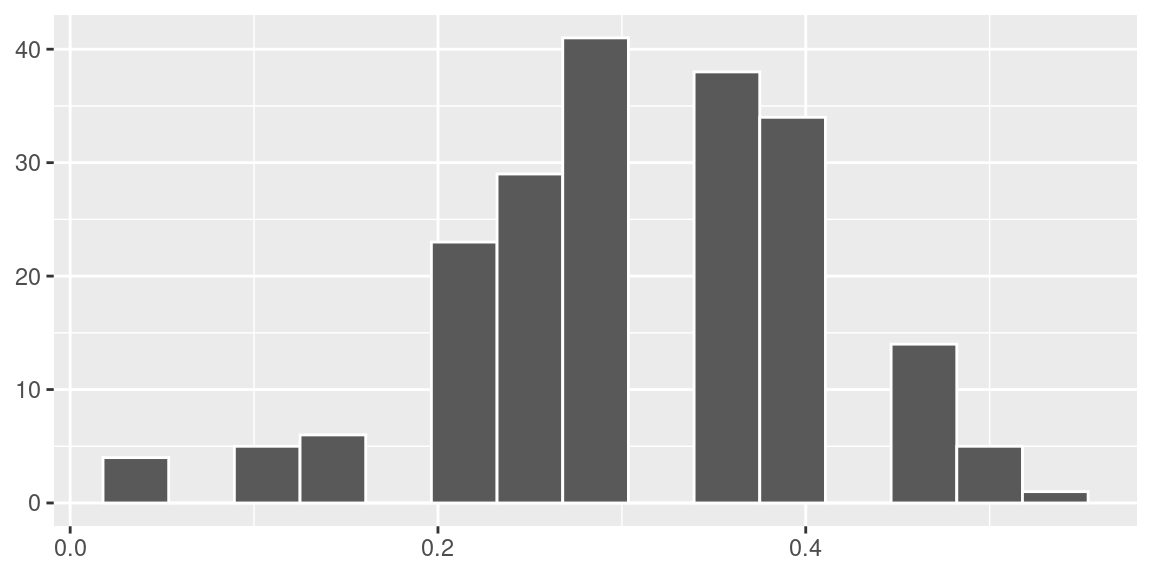
\includegraphics{inferencia_com_R_files/figure-latex/unnamed-chunk-55-1} \end{center}

Nessa simulação obtivemos \(\hat p =\) 0.29.

Suponha agora que façamos o mesmo processo, porém ao invés de considerarmos 15 amostras de tamanho 20, consideramos 200 amostras.

\begin{Shaded}
\begin{Highlighting}[]
\NormalTok{n }\OtherTok{=} \DecValTok{200}
\NormalTok{matriz\_aux }\OtherTok{=} \FunctionTok{matrix}\NormalTok{(}\ConstantTok{NA}\NormalTok{,}\AttributeTok{nrow=}\DecValTok{20}\NormalTok{,}\AttributeTok{ncol=}\NormalTok{n)}
\ControlFlowTok{for}\NormalTok{(j }\ControlFlowTok{in} \DecValTok{1}\SpecialCharTok{:}\FunctionTok{ncol}\NormalTok{(matriz\_aux))\{matriz\_aux[,j]}\OtherTok{=}\FunctionTok{rbinom}\NormalTok{(}\DecValTok{20}\NormalTok{,}\DecValTok{1}\NormalTok{,}\AttributeTok{prob=}\FloatTok{0.3}\NormalTok{)\}}
\NormalTok{medias }\OtherTok{=} \FunctionTok{data.frame}\NormalTok{(}\AttributeTok{x=}\DecValTok{1}\SpecialCharTok{:}\FunctionTok{ncol}\NormalTok{(matriz\_aux),}\AttributeTok{y=}\FunctionTok{colMeans}\NormalTok{(matriz\_aux))}
\FunctionTok{ggplot}\NormalTok{(medias,}\FunctionTok{aes}\NormalTok{(y)) }\SpecialCharTok{+}
  \FunctionTok{geom\_histogram}\NormalTok{(}\AttributeTok{color =} \StringTok{"white"}\NormalTok{, }\AttributeTok{bins =} \DecValTok{15}\NormalTok{) }\SpecialCharTok{+}
  \FunctionTok{theme}\NormalTok{(}\AttributeTok{axis.title =} \FunctionTok{element\_blank}\NormalTok{())}
\end{Highlighting}
\end{Shaded}

\begin{center}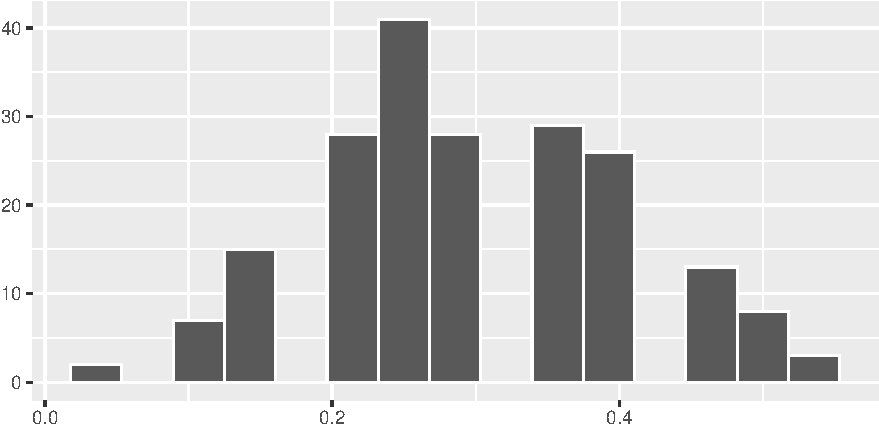
\includegraphics{inferencia_com_R_files/figure-latex/unnamed-chunk-56-1} \end{center}

Agora, obtivemos \(\hat p =\) 0.29.

Realizando o mesmo experimento, porém agora considerando 10000 amostras de tamanho 20, a distribuição da média amostral pode ser vista segundo o histograma abaixo.

\begin{Shaded}
\begin{Highlighting}[]
\NormalTok{n }\OtherTok{=} \DecValTok{10000}
\NormalTok{matriz\_aux }\OtherTok{=} \FunctionTok{matrix}\NormalTok{(}\ConstantTok{NA}\NormalTok{,}\AttributeTok{nrow=}\DecValTok{20}\NormalTok{,}\AttributeTok{ncol=}\NormalTok{n)}
\ControlFlowTok{for}\NormalTok{(j }\ControlFlowTok{in} \DecValTok{1}\SpecialCharTok{:}\FunctionTok{ncol}\NormalTok{(matriz\_aux))\{matriz\_aux[,j]}\OtherTok{=}\FunctionTok{rbinom}\NormalTok{(}\DecValTok{20}\NormalTok{,}\DecValTok{1}\NormalTok{,}\AttributeTok{prob=}\FloatTok{0.3}\NormalTok{)\}}
\NormalTok{medias }\OtherTok{=} \FunctionTok{data.frame}\NormalTok{(}\AttributeTok{x=}\DecValTok{1}\SpecialCharTok{:}\FunctionTok{ncol}\NormalTok{(matriz\_aux),}\AttributeTok{y=}\FunctionTok{colMeans}\NormalTok{(matriz\_aux))}
\FunctionTok{ggplot}\NormalTok{(medias,}\FunctionTok{aes}\NormalTok{(y)) }\SpecialCharTok{+}
  \FunctionTok{geom\_histogram}\NormalTok{(}\AttributeTok{color =} \StringTok{"white"}\NormalTok{, }\AttributeTok{bins =} \DecValTok{15}\NormalTok{) }\SpecialCharTok{+}
  \FunctionTok{theme}\NormalTok{(}\AttributeTok{axis.title =} \FunctionTok{element\_blank}\NormalTok{())}
\end{Highlighting}
\end{Shaded}

\begin{center}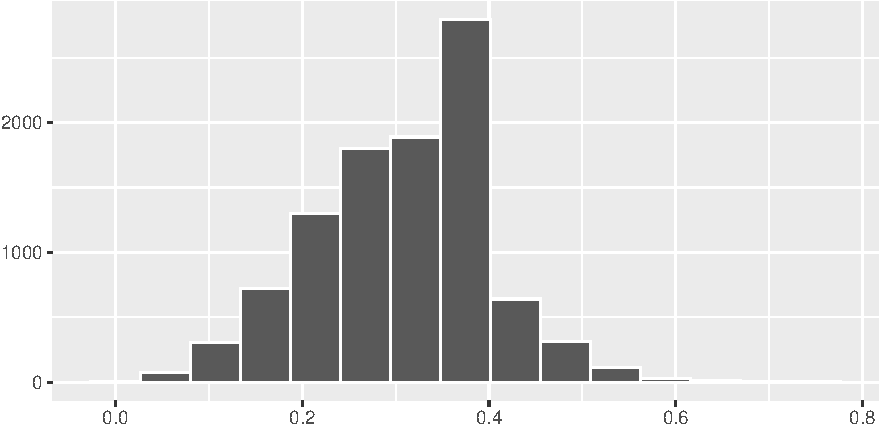
\includegraphics{inferencia_com_R_files/figure-latex/unnamed-chunk-57-1} \end{center}

Para este caso, a média das proporções amostrais foi \(\hat p=\) 0.3. Então, empiricamente, podemos perceber que a distribuição da média amostral se aproxima de uma distribuição normal com média \(\mu=0,3\) e desvio padrão \(\frac{p(1-p)}{\sqrt{n}}=\frac{0.21}{\sqrt{20}}=0,0105\).

\hypertarget{intervalo-de-confianuxe7a}{%
\chapter{Intervalo de Confiança}\label{intervalo-de-confianuxe7a}}

\hypertarget{ideia-geral}{%
\section{Ideia Geral}\label{ideia-geral}}

Neste capítulo você aprenderá um método muito importante de estimação de parâmetros. Vimos anteriormente que a média amostral \(\bar X\) é um bom estimador da média populacional \(\mu\). Mas vimos, também, que existe uma variabilidade nos valores de \(\bar X\), ou seja, cada amostra dá origem a um valor diferente do estimador. Uma maneira de informar sobre esta variabilidade é através da estimação por intervalos.

O objetivo central da inferência estatística é obter informações para uma população a partir do conhecimento de uma única amostra. Em geral, a população é representada por uma variável aleatória \(X\), com função de distribuição ou densidade de probabilidade \(f_X\) . Dessa população, então, extrai-se uma amostra aleatória simples com reposição, que dá origem a um conjunto \(X_1, X_2, \ldots, X_n\) de \(n\) variáveis aleatórias independentes e identicamente distribuídas, todas com a mesma distribuição \(f_X\).

Se \(f_X\) depende de um ou mais parâmetros, temos que usar a informação obtida a partir da amostra para estimar esses parâmetros, de forma a conhecermos a distribuição. Vimos, por exemplo, que a média amostral \(\bar X\) é um bom estimador da média populacional \(\mu\), no sentido de que ela tende a ``acertar o alvo'' da verdadeira média populacional, isto é, a média amostral é um estimador não-viesado da média populacional. Mas vimos, também, que existe uma variabilidade nos valores de \(\bar X\), ou seja, cada amostra dá origem a um valor diferente do estimador. Para algumas amostras, \(\bar X\) será maior que \(\mu\), para outras será menor e para outras será igual.

Na prática, temos apenas uma amostra e, assim, é importante que se dê alguma informação sobre essa possível variabilidade do estimador. Ou seja, é importante informar o valor do estimador \(\hat \theta\) obtido com uma amostra específica, mas é importante informar também que o verdadeiro valor do parâmetro \(\theta\) poderia estar num determinado intervalo, digamos, no intervalo \(\left[\hat\theta-\varepsilon,\hat\theta+\varepsilon\right]\). Dessa forma, estamos informando a nossa margem de erro no processo de estimação; essa margem de erro é consequência do processo de seleção aleatória da amostra.

O que vamos estudar agora é como obter esse intervalo, de modo a ``acertar na maioria das vezes'', isto é, queremos um procedimento que garanta que, na maioria das vezes (ou das amostras possíveis), o intervalo obtido conterá o verdadeiro valor do parâmetro. A expressão ``na maioria das vezes'' será traduzida como ``probabilidade alta''. Dessa forma, estaremos lidando com afirmativas do seguinte tipo:

\textbf{Com probabilidade alta (em geral, indicada por $1-\alpha$), o intervalo $\left[\hat\theta-\varepsilon,\hat\theta+\varepsilon\right]$ conterá o verdadeiro valor do parâmetro $\theta$.}

A interpretação correta de tal afirmativa é a seguinte: se \(1-\alpha=0,95\), por exemplo, então isso significa que o procedimento de construção do intervalo é tal que, em 95\% das possíveis amostras, o intervalo \(\left[\hat\theta-\varepsilon,\hat\theta+\varepsilon\right]\) obtido conterá o verdadeiro valor do parâmetro.

Note, no exemplo abaixo, que cada amostra resulta em um intervalo diferente, mas em média, em 95\% das amostras, o intervalo contém o verdadeiro valor do parâmetro (em vermelho).

\begin{center}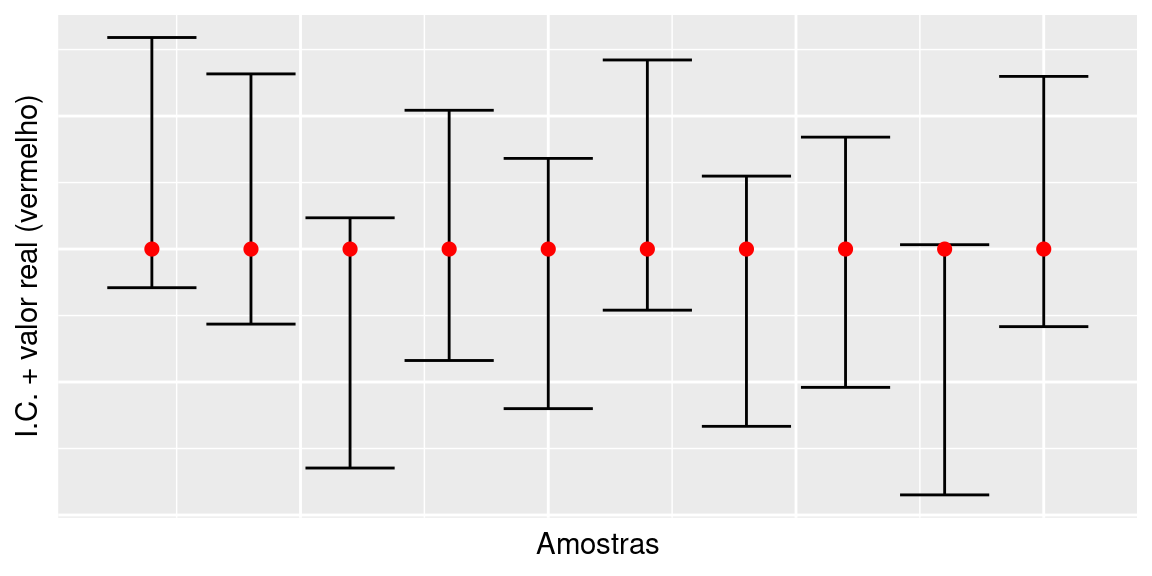
\includegraphics{inferencia_com_R_files/figure-latex/unnamed-chunk-58-1} \end{center}

O valor \(1 - \alpha\) é chamado nível de confiança, enquanto o valor \(\alpha\) é conhecido como nível de significância. O intervalo \(\left[\hat\theta-\varepsilon;\hat\theta + \varepsilon\right]\) é chamado de intervalo de confiança de nível de confiança \(1 - \alpha\).

Tendo clara a interpretação do intervalo de confiança, podemos resumir a frase acima da seguinte forma:

\[P\left(\theta\in[\hat\theta-\varepsilon;\hat\theta+\varepsilon]\right)=1-\alpha\]

Mais uma vez, a probabilidade se refere à probabilidade dentre as diversas possíveis amostras, ou seja, a probabilidade está associada à distribuição amostral de \(\hat \theta\). Note que os limites do intervalo dependem de \(\hat theta\), que depende da amostra sorteada, ou seja, os limites do intervalo de confiança são variáveis aleatórias. Cada amostra dá origem a um intervalo diferente, mas o procedimento de obtenção dos intervalos garante probabilidade \(1 - \alpha\) de acerto.

\hypertarget{i.c.-para-a-muxe9dia-de-uma-normal-com-variuxe2ncia-conhecida}{%
\section{I.C. para a média de uma Normal com variância conhecida}\label{i.c.-para-a-muxe9dia-de-uma-normal-com-variuxe2ncia-conhecida}}

Vamos agora introduzir os métodos para obtenção do intervalo de confiança para a média de uma população. Como visto, a média populacional é um parâmetro importante que pode ser muito bem estimado pela média amostral \(\bar X\). Para apresentar as idéias básicas, vamos considerar um contexto que é pouco frequente na prática. O motivo para isso é que, em termos didáticos, a apresentação é bastante simples. Como o fundamento é o mesmo para contextos mais gerais, essa abordagem se justifica.

Consideremos uma população descrita por uma variável aleatória normal com média \(\mu\) e variância \(\sigma^2\): \(X\sim N(\mu,\sigma^2)\). Vamos supor que o valor de \(\sigma^2\) seja conhecido e que nosso interesse seja estimar a média \(\mu\) a partir de uma amostra aleatória simples \(X_1,\ldots,X_n\). Como visto anteriormente, a distribuição amostral de \(\bar X\) é normal com média \(\mu\) e variância \(\frac{\sigma^2}{n}\), ou seja

\[X\sim N(\mu,\sigma^2)\rightarrow \bar X \sim N\left(\mu,\frac{\sigma^2}{n}\right)\]

Da definição de distribuição amostral, isso significa que os diferentes valores de \(\bar X\) obtidos a partir das diferentes possíveis amostras se distribuem normalmente em torno de \(\mu\) com variância \(\frac{\sigma^2}{n}\).

Das propriedades da distribuição normal, resulta que

\[Z=\frac{\bar X-\mu}{\sqrt{\frac{\sigma^2}{n}}}\sim N(0,1),\]

ou equivalentemente,

\[Z=\sqrt{n}\frac{\bar X-\mu}{\sigma}\sim N(0,1).\]

\hypertarget{construindo-o-intervalo-de-confianuxe7a}{%
\subsection{Construindo o intervalo de confiança}\label{construindo-o-intervalo-de-confianuxe7a}}

Vamos indicar por \(z_\alpha\) a abscissa da curva normal padrão que deixa probabilidade (área) igual a \(\alpha\) acima dela. Veja a Figura abaixo. Temos, então, que \(P(Z > z_\alpha)= \alpha\). Essa abscissa \(z_\alpha\) é normalmente chamada de valor crítico.

\begin{center}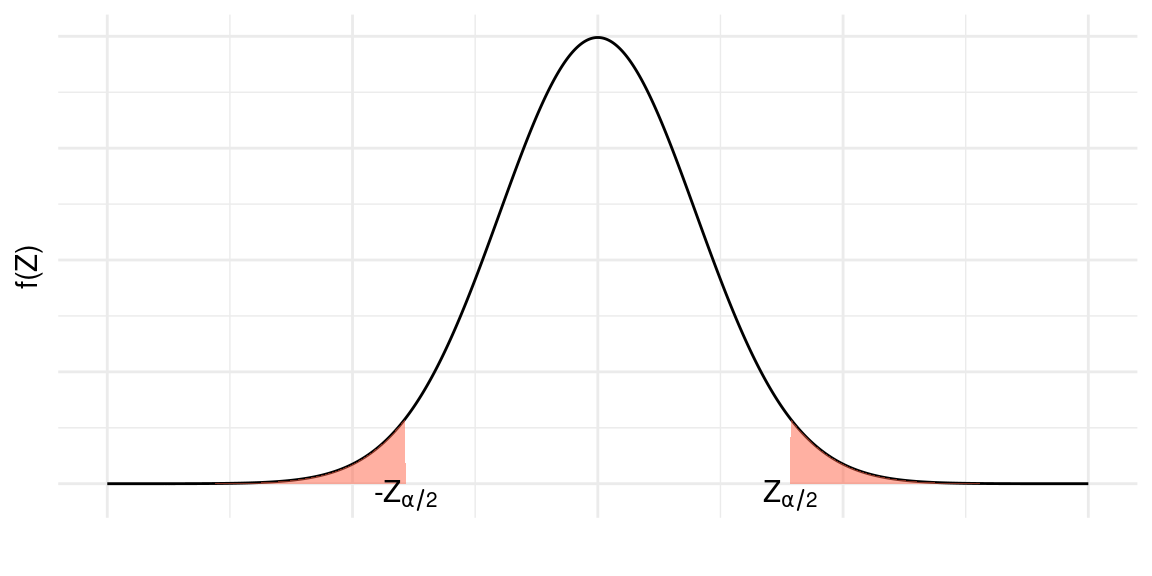
\includegraphics{inferencia_com_R_files/figure-latex/unnamed-chunk-59-1} \end{center}

Consideremos, agora, o valor crítico \(z_\frac{\alpha}{2}\), veja a Figura abaixo. Daí podemos ver que, se \(Z\sim N(0,1)\), então

\[P\left(-z_\frac{\alpha}{2}\leq Z \leq z_\frac{\alpha}{2}\right)=1-\alpha\]

\begin{center}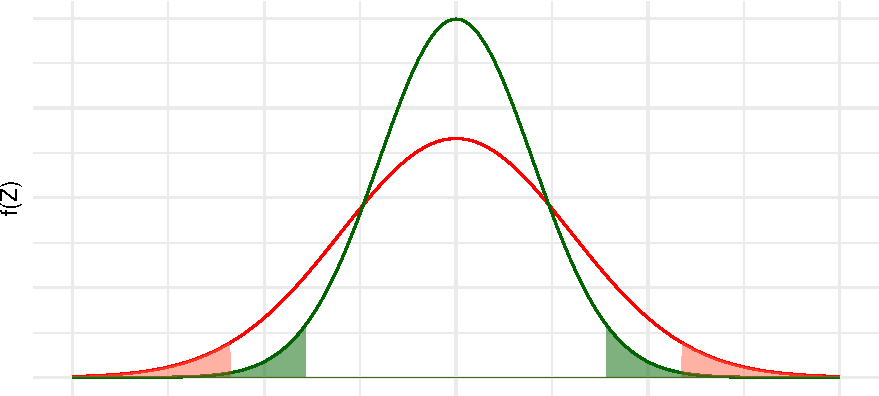
\includegraphics{inferencia_com_R_files/figure-latex/unnamed-chunk-60-1} \end{center}

Note que isso vale para a distribuição normal padrão, em geral. Então, usando os resultados anteriories obtemos que

\[P\left(-z_\frac{\alpha}{2}\leq \sqrt{n}\frac{\bar X-\mu}{\sigma} \leq z_\frac{\alpha}{2}\right)=1-\alpha\]

Mas isso é equivalente a

\[P\left(-z_{\frac{\alpha}{2}}\frac{\sigma}{\sqrt{n}}\leq \bar X-\mu \leq z_{\frac{\alpha}{2}}\frac{\sigma}{\sqrt{n}}\right)= 1-\alpha\]

\[P\left(-\bar X-z_{\frac{\alpha}{2}}\frac{\sigma}{\sqrt{n}}\leq -\mu \leq -\bar X + z_{\frac{\alpha}{2}}\frac{\sigma}{\sqrt{n}}\right)= 1-\alpha\]

\[P\left(\bar X - z_{\frac{\alpha}{2}}\frac{\sigma}{\sqrt{n}} \leq \mu \leq \bar X+z_{\frac{\alpha}{2}}\frac{\sigma}{\sqrt{n}}\right) = 1-\alpha\]

Note que a última expressão nos diz que

\[P\left(\mu \in \left[\bar X-z_{\frac{\alpha}{2}}\frac{\sigma}{\sqrt{n}};\bar X+z_{\frac{\alpha}{2}}\frac{\sigma}{\sqrt{n}}\right]\right)=1-\alpha\]

Mas essa é exatamente a forma geral de um intervalo de confiança, conforme explicitado. Temos, então, a seguinte conclusão:

Seja \(X\sim N(\mu, \sigma^2)\) uma população normal com variância \(\sigma^2\) conhecida. Se \(X_1, X_2,\ldots , X_n\) é uma amostra aleatória dessa população, então o intervalo de confiança de nível de confiança \(1-\alpha\) para a média populacional \(\mu\) é dado por

\[\left[\bar X-z_{\frac{\alpha}{2}}\frac{\sigma}{\sqrt{n}};\bar X+z_{\frac{\alpha}{2}}\frac{\sigma}{\sqrt{n}}\right],\]

onde \(z_{\frac{\alpha}{2}}\) é a abscissa da curva normal padrão que deixa a área \(\frac{\alpha}{2}\) acima dela.

\hypertarget{margem-de-erro}{%
\subsection{Margem de Erro}\label{margem-de-erro}}

O intervalo de confiança para \(\mu\) pode ser escrito na forma \(\left[\bar X - \varepsilon;\bar X + \varepsilon \right]\) onde \(\varepsilon=z_{\frac{\alpha}{2}}\frac{\sigma}{\sqrt{n}}\) é a margem de erro.

Analisando a margem de erro, podemos ver que ela depende diretamente do valor crítico e do desvio padrão populacional e é inversamente proporcional ao tamanho da amostra.

Na Figura abaixo ilustra-se a relação de dependência da margem de erro em relação ao desvio padrão populacional \(\sigma\). Temos aí duas distribuições amostrais centradas na mesma média e baseadas em amostras de mesmo tamanho. Nas duas distribuições a área total das caudas sombreadas é \(\alpha\), de modo que o intervalo limitado pelas linhas verticais é o intervalo de confiança de nível de confiança \(1-\alpha\). Para a distribuição mais dispersa, isto é, com \(\sigma\) maior, o comprimento do intervalo é maior. Esse resultado deve ser intuitivo: se há mais variabilidade na população, a nossa margem de erro tem que ser maior, mantidas fixas as outras condições (tamanho de amostra e nível de confiança).

\begin{center}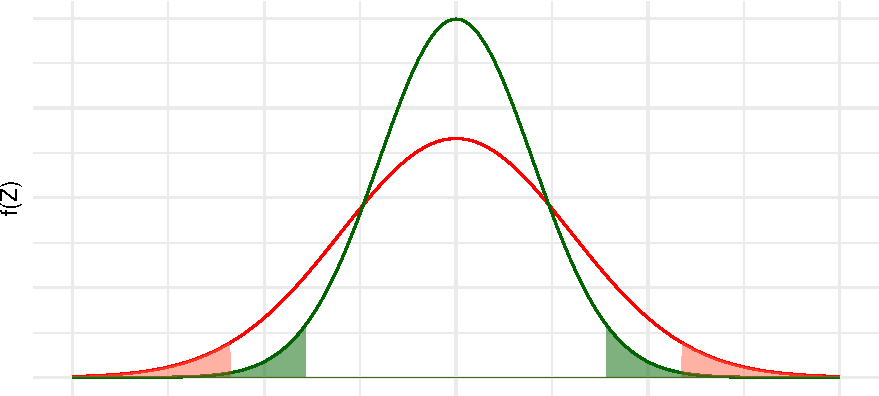
\includegraphics{inferencia_com_R_files/figure-latex/unnamed-chunk-61-1} \end{center}

Por outro lado, se mantivermos fixos o tamanho da amostra e o desvio padrão populacional, é razoável também esperar que a margem de erro seja maior para um nível de confiança maior. Ou seja, se queremos aumentar a probabilidade de acerto, é razoável que o intervalo seja maior. Aumentar a probabilidade de acerto significa aumentar o nível de confiança, o que acarreta em um valor crítico \(z_{\frac{\alpha}{2}}\) maior.

Finalmente, mantidos o mesmo desvio padrão populacional e o mesmo nível de confiança, quanto maior o tamanho da amostra, mais perto vamos ficando da população e, assim, vai diminuindo a nossa margem de erro.

\hypertarget{determinauxe7uxe3o-do-tamanho-da-amostra}{%
\subsection{Determinação do tamanho da amostra}\label{determinauxe7uxe3o-do-tamanho-da-amostra}}

XXX

\hypertarget{i.c.-para-a-muxe9dia-de-uma-normal-com-variuxe2ncia-desconhecida}{%
\section{I.C. para a média de uma Normal com variância desconhecida}\label{i.c.-para-a-muxe9dia-de-uma-normal-com-variuxe2ncia-desconhecida}}

Nesta seção você completará seu estudo básico sobre intervalos de confiança para a média de uma população, analisando o problema de estimação da média de uma população normal quando não se conhece a variância desta população. Você verá que, neste caso, é necessário estimar essa variância e isso introduz mais uma fonte de variabilidade nas nossas estimativas: com uma única amostra, temos que estimar a média e a variância da população. O procedimento é simples e análogo aos casos anteriores vistos nos capítulos amteriores; o que muda é a distribuição amostral do estimador \(\bar X\). Em vez de usarmos a distribuição normal para determinar os valores críticos, usaremos a distribuição \(t\) de Student.

Considere uma população descrita por uma variável aleatória normal com média \(\mu\) e variância \(\sigma^2\): \(X\sim N(\mu,\sigma^2)\). Nosso interesse é estimar a média \(\mu\) a partir de uma amostra aleatória simples \(X_1,X_2,\ldots,X_n\). Como visto anteriormente, a distribuição amostral de \(\bar X\) é normal com média \(\mu\) e variância \(\frac{\sigma^2}{n}\), ou seja

\[X\sim N(\mu,\sigma^2)\rightarrow \bar X \sim N\left(\mu,\frac{\sigma^2}{n}\right)\]
No entanto, agora, a variância \(\sigma^2\) não é conhecida. Neste caso, temos que estimá-la (\(S^2\)) com os dados amostrais. Foi demostrado que

\[S^2=\frac{1}{n-1}\sum_{i=1}^{n}(X_i-\bar X)^2=\frac{1}{n-1}\left[\sum_{i=1}^{n}X_i^2-n\bar X^2\right]\]

é um estimador não viesado para \(\sigma^2\). Isso significa que, se calculássemos o valor de \(S^2\) para cada uma das possíveis amostras aleatórias simples de tamanho \(n\), a média desses valores seria igual a \(\sigma^2\). Dessa forma, \(S^2\) é um ``bom'' estimador de \(\sigma^2\) e podemos usá-lo como uma estimativa pontual de \(\sigma^2\). Como o desvio padrão é a raiz quadrada da variância, é natural perguntar: \(S\) é um ``bom'' estimador de \(\sigma\), ou seja, \(S\) é um estimador não-viesado de \(\sigma\)? A resposta é NÃO, mas, para grandes amostras, o viés é pequeno, de modo que, em geral, usa-se \(S\) como estimador de \(\sigma\). Sendo assim, é natural pensarmos em substituir o valor de \(\sigma\) por \(S\) na expressão da Normal \(Z\) e utilizarmos a estatística

\[T=\sqrt{n}\frac{\bar X-\mu}{S}\]

na construção de intervalos de confiança para \(\mu\). Isso é exatamente o que faremos, mas, ao introduzirmos \(S\) no lugar de \(\sigma\), a distribuição amostral de \(T\) deixa de ser normal e passa a ser uma distribuição \(t\) de Student.

O intervalo de confiança para a média de uma população normal com variância desconhecida é obtido com base no seguinte resultado:

\[T=\sqrt{n}\frac{\bar X-\mu}{S}\sim t_{n-1},\]

onde \(S^2=\frac{1}{n-1}\sum_{i=1}^{n}(X_i-\bar X)^2=\frac{1}{n-1}\left[\sum_{i=1}^{n}X_i^2-n\bar X^2\right].\)

O número de graus de liberdade \(gl=n-1\) resulta do fato de que, na soma que define \(S^2\), há apenas \(n-1\) parcelas independentes, ou seja, dados \(S^2\) e \(n-1\) das parcelas \((X_i - \bar X)^2\), a \(n\)-ésima parcela fica automaticamente determinada.

\hypertarget{construindo-o-intervalo-de-confianuxe7a-1}{%
\subsection{Construindo o intervalo de confiança}\label{construindo-o-intervalo-de-confianuxe7a-1}}

Vamos indicar por \(t_\alpha\) a abscissa da curva t-student que deixa probabilidade (área) igual a \(\alpha\) acima dela, portanto \(t_\frac{\alpha}{2}\) deixa \(\frac{\alpha}{2}\) acima. Veja a Figura abaixo. Temos, então, que \(P(T > t_\frac{\alpha}{2})= \frac{\alpha}{2}\). Essa abscissa \(t_\frac{\alpha}{2}\) é normalmente chamada de valor crítico.

\begin{center}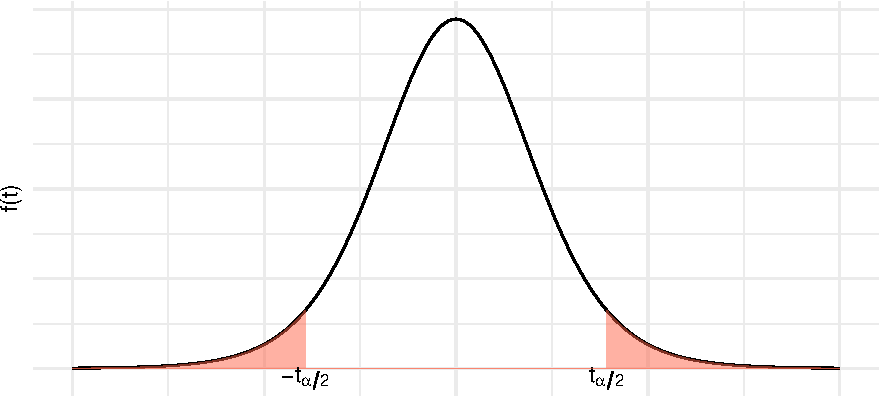
\includegraphics{inferencia_com_R_files/figure-latex/unnamed-chunk-62-1} \end{center}

Usando a simetria da densidade \(t\), temos o seguinte resultado:

\[P\left(-t_{n,\alpha/2}\leq t_{n} \leq t_{n,\alpha/2}\right)=1-\alpha\]

Note que isso vale para a distribuição \(t\) de student, em geral. Então, usando os resultados anteriores obtemos que

\[P\left(-t_{n-1,\alpha/2}\leq \sqrt{n}\frac{\bar X-\mu}{S} \leq t_{n-1,\alpha/2}\right)=1-\alpha\]

Mas isso é equivalente a

\[P\left(-t_{n-1,\alpha/2}\frac{S}{\sqrt{n}}\leq \bar X-\mu \leq t_{n-1,\alpha/2}\frac{S}{\sqrt{n}}\right)=1-\alpha\]
\[P\left(\bar X-t_{n-1,\alpha/2}\frac{S}{\sqrt{n}}\leq \mu \leq \bar X + t_{n-1,\alpha/2}\frac{S}{\sqrt{n}}\right)=1-\alpha\]

Note que a última expressão nos diz que

\[P\left(\mu \in \left[\bar X-t_{n-1,\alpha/2}\frac{S}{\sqrt{n}};\bar X+t_{n-1,\alpha/2}\frac{S}{\sqrt{n}}\right]\right)=1-\alpha\]

Mas essa é exatamente a forma geral de um intervalo de confiança, conforme explicitado. Temos, então, a seguinte conclusão:

Seja \(X\sim N(\mu, \sigma^2)\) uma população normal com variância \(\sigma^2\) desconhecida. Se \(X_1, X_2,\ldots , X_n\) é uma amostra aleatória dessa população, então o intervalo de confiança de nível de confiança \(1-\alpha\) para a média populacional \(\mu\) é dado por

\[\left[\bar X-t_{n-1,\alpha/2}\frac{S}{\sqrt{n}};\bar X+t_{n-1,\alpha/2}\frac{S}{\sqrt{n}}\right],\]

onde \(t_{n-1,\alpha/2}\) é o valor crítico da distribuição \(t\) de student com \(n-1\) graus de liberdade que deixa a área \(\frac{\alpha}{2}\) acima dela.

\hypertarget{margem-de-erro-1}{%
\subsection{Margem de Erro}\label{margem-de-erro-1}}

Note, mais uma vez, a forma do intervalo de confiança:

\[\bar X \pm\varepsilon,\]

onde a margem de erro \(\varepsilon\), agora é definida em termos do valor crítico da distribuição \(t\) e do erro padrão estimado de \(\bar X\):

\[\varepsilon=t_{n-1,\alpha/2}\frac{S}{\sqrt{n}}\].

\hypertarget{determinauxe7uxe3o-do-tamanho-da-amostra-1}{%
\subsection{Determinação do tamanho da amostra}\label{determinauxe7uxe3o-do-tamanho-da-amostra-1}}

XXX

\hypertarget{i.c.-para-a-proporuxe7uxe3o-populacional}{%
\section{I.C. para a proporção populacional}\label{i.c.-para-a-proporuxe7uxe3o-populacional}}

Anteriormente, foram apresentadas as idéias básicas da estimação por intervalos de confiança. Para ilustrar o princípio utilizado na construção de tais intervalos, consideramos a situação especial de estimação da média de uma população normal com variância conhecida. Neste caso, a distribuição amostral da média amostral é normal e foi com base nessa distribuição amostral normal que obtivemos o intervalo de confiança.

No primeiro momento desta seção usaremos o Teorema Central do Limite, que garante que a distribuição amostral da proporção amostral pode ser aproximada por uma distribuição normal, desde que utilizemos amostras grandes.

O contexto de interesse é o seguinte: temos uma população em que cada elemento é classificado de acordo com a presença ou ausência de determinada característica. Em termos de variável aleatória, essa população é representada por uma v.a. de Bernoulli, isto é:

\[
X=\begin{cases}
1,~\text{se elemento possui a característica de interesse}\\
0,~\text{se elemento não possui a caracaterística de interesse}
\end{cases}
\]

Então, \(P(X = 1) = p\), \(E(X) = p\) e \(V(X) = p(1 - p)\). O parâmetro \(p\) é também a proporção de elementos da população que possuem a caracterísitca de interesse. Em geral, esse parâmetro é desconhecido e precisamos estimá-lo a partir de uma amostra.

Suponha, então, que dessa população seja extraída uma amostra aleatória simples \(X_1, X_2, \ldots, X_n com reposição\). Vimos que a proporção \(\hat P\) de elementos na amostra que possuem a característica de interesse, definida por

\[\hat P = \frac{S_n}{n}=\frac{X_1+X_2+\ldots+X_n}{n}\]

é um estimador não-viesado para \(p\) com variância \(\frac{p(1-p)}{n}\). Mais precisamente,

\[E(\hat P)=p\]

\[V(\hat P)=\frac{p(1-p)}{n}\]

Como a proporção amostral é uma média de uma amostra aleatória simples de uma população com distribuição de Bernoulli com parâmetro \(p\), o Teorema Limite Central nos diz que a distribuição de \(\hat P\) se aproxima de uma nornal com média \(p\) e variância \(\frac{p(1-p)}{n}\).

Resumindo, temos o seguinte resultado:

\[\hat p \sim N\left(p,\frac{p(1-p)}{n}\right).\]

Usando as propriedades da distribuição normal, temos que

\[\frac{\hat P - p}{\sqrt{\frac{p(1-p)}{n}}}\sim N(0,1)\]

ou equivalentemente

\[\sqrt{n}\frac{\hat P - p}{\sqrt{p(1-p)}}\sim N(0,1)\]

Vamos ver, agora, como usar esse resultado para obter um intervalo de confiança para a verdadeira proporção populacional \(p\).

\hypertarget{construindo-o-intervalo-de-confianuxe7a-2}{%
\subsection{Construindo o intervalo de confiança}\label{construindo-o-intervalo-de-confianuxe7a-2}}

O procedimento de construção do intervalo de confiança para a proporção populacional é totalmente análogo ao do intervalo de confiança para a média de uma população normal com variância conhecida, visto anteriormente. Assim, iremos usar a mesma notação, a saber: vamos representar por \(z_\alpha\) a abscissa da curva normal padrão que deixa probabilidade (área) \(\alpha\) acima dela. Como visto, temos o seguinte resultado, onde \(Z\sim N(0,1)\):

\[P\left(-z_\frac{\alpha}{2}\leq Z \leq z_\frac{\alpha}{2}\right)=1-\alpha\]

Como o resultado acima vale para qualquer variável aleatória \(N(0,1)\), podemos usar para obter

\[P\left(-z_{\frac{\alpha}{2}}\leq \frac{\hat P - p}{\sqrt{\frac{p(1-p)}{n}}} \leq z_{\frac{\alpha}{2}}\right)=1-\alpha\]

e, portanto

\[P\left(-z_{\frac{\alpha}{2}}\sqrt{\frac{p(1-p)}{n}} \leq \hat P - p \leq z_{\frac{\alpha}{2}}\sqrt{\frac{p(1-p)}{n}}\right)=1-\alpha\]

\[P\left(-\hat P -z_{\frac{\alpha}{2}}\sqrt{\frac{p(1-p)}{n}} \leq - p \leq -\hat P + z_{\frac{\alpha}{2}}\sqrt{\frac{p(1-p)}{n}}\right)=1-\alpha\]

\[P\left(\hat P - z_{\frac{\alpha}{2}}\sqrt{\frac{p(1-p)}{n}} \leq p \leq \hat P + z_{\frac{\alpha}{2}}\sqrt{\frac{p(1-p)}{n}}\right)=1-\alpha\]

Como no caso da média, chegamos a uma expressão do seguinte tipo:

\[P(\hat P -\varepsilon\leq p\leq\hat P + \varepsilon)=1-\alpha\]

onde \(\varepsilon=z_{\frac{\alpha}{2}}\sqrt{\frac{p(1-p)}{n}}\)

\hypertarget{margem-de-erro-2}{%
\subsection{Margem de Erro}\label{margem-de-erro-2}}

Analisando a margem de erro, podemos ver uma diferença fundamental entre o IC para a proporção e para a média: a margem de erro da proporção amostral depende do parâmetro desconhecido \(p\). Na prática, para construir o intervalo de confiança, temos que substituir esse valor por alguma estimativa.

Existem 3 abordagens possíveis:

\begin{enumerate}
\def\labelenumi{\arabic{enumi}.}
\item
  Usar a própria proporção amostral observada; nesse caso, o intervalo de confiança seria: \[\hat p \pm z_{\frac{\alpha}{2}}\sqrt{\frac{\hat p(1-\hat p)}{n}}\]
\item
  Usar o intervalo de confiança conservador, ou seja, usar o maior valor possível para \(z_{\frac{\alpha}{2}}\sqrt{\frac{\hat p(1-\hat p)}{n}}\) para um dado \(n\), o que equivale a obter o intervalo de confiança com o maior comprimento possível. Como o comprimento do intervalo é diretamente proporcional a \(\sqrt{p(1-p)}\) ou equivalentemente a \(p(1-p)\), \(p=0.5\) maxima esta função.
\end{enumerate}

Neste caso, o o intervalo de confiança se torna:

\[\hat p \pm z_{\frac{\alpha}{2}}\sqrt{\frac{0.5\times 0.5}{n}} = \hat p \pm z_{\frac{\alpha}{2}}\frac{0.5}{\sqrt{n}}\]

\begin{enumerate}
\def\labelenumi{\arabic{enumi}.}
\setcounter{enumi}{2}
\tightlist
\item
  Usar algum valor auxiliar \(\hat p_0\) ou estimativa prévia, obtida de outras fontes ou de uma amostra piloto:
\end{enumerate}

\[\hat p \pm z_{\frac{\alpha}{2}}\sqrt{\frac{\hat p_0(1-\hat p_0)}{n}}\]

Seja \(X\sim Bernoulli(p)\). Se \(X_1,X_2,\ldots,X_n\) é uma amostra aleatória dessa população, então o intervalo de confiança de nível de confiança \(1-\alpha\) para a proporção populacional \(p\) é dado por

\[\left[\hat P - z_{\frac{\alpha}{2}}\sqrt{\frac{\hat p_0(1-\hat p_0)}{n}};\hat P + z_{\frac{\alpha}{2}}\sqrt{\frac{\hat p_0(1-\hat p_0)}{n}}\right],\]

onde \(z_{\frac{\alpha}{2}}\) é a abscissa da curva normal padrão que deixa a área \(\frac{\alpha}{2}\) acima dela e \(\hat p_0\) é alguma estimativa para o verdadeiro valor de \(p\).

\hypertarget{determinauxe7uxe3o-do-tamanho-da-amostra-2}{%
\subsection{Determinação do tamanho da amostra}\label{determinauxe7uxe3o-do-tamanho-da-amostra-2}}

Uma questão que se coloca freqüentemente é: qual o tamanho da amostra necessário para se estimar uma proporção \(p\) com uma margem de erro \(\varepsilon\) e nível de confiança \(1-\alpha\)? Vamos analisar a expressão da margem de erro:

\[\varepsilon=z_{\frac{\alpha}{2}}\sqrt{\frac{p(1-p)}{n}}\]

Resolvendo para \(n\), obtemos que

\[\sqrt{n}=z_{\frac{\alpha}{2}}\frac{\sqrt{p(1-p)}}{\varepsilon}\]

ou

\[n=p(1-p)\left(\frac{z_{\frac{\alpha}{2}}}{\varepsilon}\right)^2\]

Vemos, então, que \(n\) é diretamente proporcional a \(p(1-p)\), ou seja, quanto maior \(p(1-p)\), maior será o tamanho da amostra \(n\). Na prática, não conhecemos \(p\) (na verdade, estamos querendo estimar esse parâmetro). Então, para determinar o tamanho de amostra necessário para uma margem de erro e um nível de confiança dados, podemos considerar o pior caso, ou seja, podemos tomar o maior valor possível de \(p(1 - p)\) e calcular o tamanho da amostra com base nesse pior caso, que ocorre quando \(p = 0,5\). É claro que essa é uma escolha conservadora, que em alguns casos pode levar a um tamanho de amostra desnecessariamente grande. Usando esta estimativa para \(p\), obtemos que

\[n=\left(0,5\times \frac{z_{\frac{\alpha}{2}}}{\varepsilon}\right)^2\]

\hypertarget{intervalo-de-confianuxe7a-para-a-variuxe2ncia-de-uma-normal}{%
\section{Intervalo de confiança para a variância de uma Normal}\label{intervalo-de-confianuxe7a-para-a-variuxe2ncia-de-uma-normal}}

Nesta parte você completará seu estudo básico sobre intervalos de confiança, analisando o problema de estimação da variância de uma população normal. Como antes, este intervalo se baseará na distribuição amostral de um estimador não-viesado para \(\sigma^2\), a saber, \(S^2\). Como a variância é um número não negativo, essa distribuição não é simétrica e está definida apenas para valores não-negativos.

O contexto subjacente é o seguinte: a partir de uma amostra aleatória simples \(X_1,X_2,\ldots,X_n\) retirada de uma população normal com média \(\mu\) e variância \(\sigma^2\) queremos construir um intervalo de confiança para \(\sigma^2\). A hipótese de normalidade da população é fundamental aqui. Assim como no caso da média, temos que usar a distribuição amostral de algum estimador. Neste caso, o estimador é \(S^2\) e o resultado importate é o seguinte: \(\frac{(n-1)S^2}{\sigma^2}\) tem distribuição qui-quadrado com \(n-1\) graus de liberdade:

\[\frac{(n-1)S^2}{\sigma^2}\sim\chi^2_{n-1}\]

\hypertarget{construindo-o-intervalo-de-confianuxe7a-3}{%
\subsection{Construindo o intervalo de confiança}\label{construindo-o-intervalo-de-confianuxe7a-3}}

Como no caso da distribuição \(t\)-Student e também da distribuição Normal, vamos definir o valor crítico \(\chi^2_{n;\alpha}\) como a abscissa da distribuição qui-quadrado com \(n\) graus de liberdade que deixa probabilidade \(\alpha\) acima dela.

\begin{center}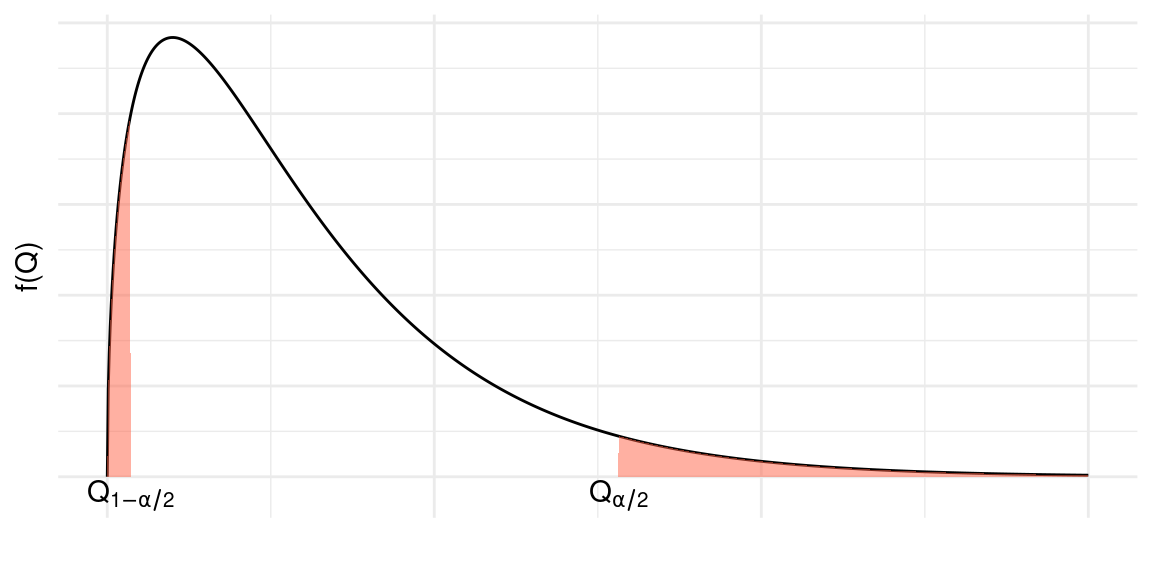
\includegraphics{inferencia_com_R_files/figure-latex/unnamed-chunk-63-1} \end{center}

Com essa definição, podemos ver que a abscissa \(\chi^2_{n;\alpha/2}\) deixa probabilidade \(\alpha/2\) acima dela e a abscissa \(\chi^2_{n;1-\alpha/2}\) deixa probabilidade \(\alpha/2\) abaixo dela.

\begin{center}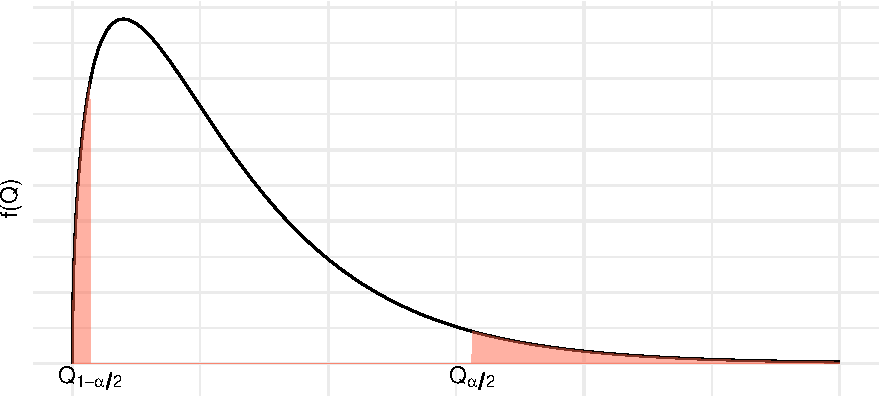
\includegraphics{inferencia_com_R_files/figure-latex/unnamed-chunk-64-1} \end{center}

Logo,

\[P\left(\chi^2_{n;\frac{\alpha}{2}}\leq \chi^2_{n} \leq \chi^2_{n;1-\frac{\alpha}{2}}\right)=1-\alpha\]

Como o resultado acima vale para qualquer distribuição qui-quadrado, podemos usar o resultado anterior para escrever

\[P\left(\chi^2_{n-1;\frac{\alpha}{2}}\leq \frac{(n-1)S^2}{\sigma^2} \leq \chi^2_{n-1;1-\frac{\alpha}{2}}\right)=1-\alpha\]

Daí resulta que

\[P\left(\frac{\chi^2_{n-1;\frac{\alpha}{2}}}{(n-1)S^2}\leq \frac{1}{\sigma^2} \leq \frac{\chi^2_{n-1;1-\frac{\alpha}{2}}}{(n-1)S^2}\right)=1-\alpha\]

\[P\left(\frac{(n-1)S^2}{\chi^2_{n-1;1-\frac{\alpha}{2}}}\leq \sigma^2 \leq \frac{(n-1)S^2}{\chi^2_{n-1;\frac{\alpha}{2}}}\right)=1-\alpha\]

e esse é o intervalo de confiança para a variância de uma população normal.

Seja \(X\sim N(\mu,\sigma^2)\) uma população normal. Se \(X_1,X_2,\ldots,X_n\) é uma amostra aleatória dessa população, então o intervalo de confiança de nível de confiança \(1-\alpha\) para a variância populacional \(\sigma^2\) é dado por

\[\left[\frac{(n-1)S^2}{\chi^2_{n-1;1-\frac{\alpha}{2}}};\frac{(n-1)S^2}{\chi^2_{n-1;\frac{\alpha}{2}}}\right],\]

onde \(\chi^2_{n-1;\frac{\alpha}{2}}\) é o valor crítico da distribuição qui-quadrado com \(n-1\) graus de liberdade que deixa a área \(\frac{\alpha}{2}\) abaixo dela e \(\chi^2_{n-1;1-\frac{\alpha}{2}}\) é o valor crítico da distribuição qui-quadrado com \(n-1\) graus de liberdade que deixa a área \(\frac{\alpha}{2}\) acima dela.

\hypertarget{margem-de-erro-3}{%
\subsection{Margem de Erro}\label{margem-de-erro-3}}

XXX

\hypertarget{determinauxe7uxe3o-do-tamanho-da-amostra-3}{%
\subsection{Determinação do tamanho da amostra}\label{determinauxe7uxe3o-do-tamanho-da-amostra-3}}

XXX

\hypertarget{teste-de-hipuxf3teses}{%
\chapter{Teste de Hipóteses}\label{teste-de-hipuxf3teses}}

Vimos que é possível, através de estatísticas amostrais adequadas, estimar parâmetros de uma população, dentro de um certo intervalo de confiança. Nos testes de hipóteses, ao invés de se construir um intervalo de confiança no qual se espera que o parâmetro da população esteja contido, testa-se a validade de uma afirmação sobre um parâmetro da população. Então, num teste de hipóteses, procura-se tomar decisões a respeito de uma população, com base em informações obtidas de amostras desta mesma população.

\hypertarget{ideia-geral-1}{%
\section{Ideia Geral}\label{ideia-geral-1}}

O contexto em que se baseia a teoria de teste de hipóteses é basicamente o mesmo da teoria de estimação por intervalo de confiança. Temos uma população representada por uma variável aleatória \(X\) cuja distribuição de probabilidade depende de algum parâmetro \(\theta\). O interesse agora está em testar a veracidade de alguma afirmativa sobre \(\theta\).

\hypertarget{hipuxf3tese-nula}{%
\subsection{Hipótese nula}\label{hipuxf3tese-nula}}

A hipótese nula, representada por \(H_0\), é a hipótese básica que queremos testar. Em geral, definimos a hipótese nula de modo que o nosso objetivo seja rejeitar \(H_0\). Nesse curso consideraremos apenas hipóteses nulas simples, isto é, hipóteses que estabelecem que o parâmetro de interesse é igual a um determinado valor. A forma geral é

\[H_0: \theta=\theta_0\]

Alguns exemplos são:

\[H_0: \mu=6 ~~~~~~ H_0: p=0.5 ~~~~~~ H_0: \sigma^2=25\]

O procedimento de teste de hipóteses resultará em uma \emph{regra de decisão} que nos permitirá \emph{rejeitar} ou \emph{não rejeitar} \(H_0\).

\hypertarget{hipuxf3tese-alternativa}{%
\subsection{Hipótese alternativa}\label{hipuxf3tese-alternativa}}

A hipótese alternativa, representada por \(H_1\), é a hipótese que devemos considerar no caso de rejeição da hipótese nula. A forma mais geral de \(H_1\) é a hipótese bilateral

\[H_1:\theta\ne\theta_0.\]

Porém, em algumas situações, podemos ter informação que nos permita restringir o domínio da hiótese alternativa. Temos, então, hipóteses unilaterais à esquerda

\[H_1:\theta<\theta_0\]

e hipóteses unilaterais à direita

\[H_1:\theta>\theta_0.\]

A escolha entre essas formas de hipótese alternativa se faz com base no conhecimento sobre o problema sendo considerado.

\hypertarget{estatuxedstica-de-teste}{%
\subsection{Estatística de teste}\label{estatuxedstica-de-teste}}

Assim como na construção dos intervalos de confiança, iremos usar uma estatística amostral apropriada para construir o nosso teste de hipóteses e nesse contexto, essa estatística é chamada \emph{estatística de teste}. As estatísticas de teste usuais são a média amostral \(\bar X\) e a proporção amostral \(\hat P\), que serão usadas na construção de testes sobre a média e a proporção populacionais, respectivamente.

\hypertarget{tipos-de-erro}{%
\subsection{Tipos de erro}\label{tipos-de-erro}}

O procedimento de decisão é definido em termos da hipótese nula \(H_0\) e as decisões possíveis são (i) rejeitar ou (ii) não rejeitar \(H_0\). Existem duas possibilidades de erro:

\begin{itemize}
\tightlist
\item
  Erro tipo I: rejeitar \(H_0\) quando \(H_0\) é verdadeira
\item
  Erro tipo II: não rejeitar \(H_0\) quando \(H_0\) é falsa
\end{itemize}

\hypertarget{regra-de-decisuxe3o}{%
\subsection{Regra de decisão}\label{regra-de-decisuxe3o}}

A decisão sobre a hipótese nula é tomada com base em uma regra que estabelece um conjunto de valores, chamado \emph{região crítica} (RC) ou \emph{região de rejeição}, de modo que se, o valor observado da estatística amostral cair nesse região, rejeitaremos \(H_0\); caso contrário, não rejeitaremos \(H_0\).

\hypertarget{regiuxe3o-cruxedtica}{%
\subsection{Região crítica}\label{regiuxe3o-cruxedtica}}

Em geral, a definição da região crítica é feita da seguinte forma: RC é o conjunto de valores cuja probabilidade de ocorrência é pequena sob a hipótese de veracidade de \(H_0\).

A definição de ``probabilidade pequena'' se faz através da escolha do \textbf{nível de significância} \(\alpha\) do teste, que é a \textbf{probabilidade do erro tipo I}, isto é,

\[\alpha=P(\text{erro tipo I})=P(\text{rejeitar } H_0 | H_0 \text{ verdadeira})\]

Em geral, o valor de \(\alpha\) é pequeno e as escolhas mais comuns são \(\alpha=0.05\) e \(\alpha=0.01\).

Definido o nível de significância \(\alpha\), podemos estabelecer a região crítica usando a distribuição amostral da estatística de teste.

\hypertarget{cco-e-poder-do-teste}{%
\subsection{CCO e Poder do Teste}\label{cco-e-poder-do-teste}}

No procedimento de teste de hipóteses, as decisões possíveis são rejeitar ou não rejeitar \(H_0\). Definem-se, assim, as seguintes funções em termos das probabilidades de cada uma delas. A \emph{Curva Característica da Operação} (CCO) é definida como

\[\beta(\theta)=P(\text{não rejeitar } H_0|\theta)\]

Define-se a \emph{função Poder de Teste} como

\[Q(\theta)=1-\beta(\theta)=P(\text{rejeitar } H_0|\theta)\]

Estas funções (probabilidades) estão condicionadas ao verdadeiro e desconhecido valor do parâmetro \(\theta\). Se este valor estiver no conjunto de valores definidos pela hipótese alternativa, então \(Q(\theta)\) corresponde a uma probabilidade de \textbf{acerto}: ela mede a probabilidade de se rejeitar \(H_0\) quando \(H_0\) é falsa. Por outro lado, se a hipótese nula é \(H_0: \theta=\theta_0\), então

\begin{itemize}
\tightlist
\item
  \(Q(\theta_0)=1-\beta(\theta_0)\)
\item
  \(Q(\theta_0)=1-P(\text{não rejeitar } H_0|\theta)\)
\item
  \(Q(\theta_0)=1-P(\text{não rejeitar } H_0|H_0 \text{ verdadeira})\)
\item
  \(Q(\theta_0)=P(\text{rejeitar } H_0|H_0 \text{ verdadeira})\)
\item
  \(Q(\theta_0)=\alpha\)
\end{itemize}

\hypertarget{exemplo}{%
\subsection{Exemplo}\label{exemplo}}

Consideremos uma população representada por uma variável aleatória normal com média \(\mu\) e variância 400. Deseja-se testar:

\[H_0:\mu=100~~~\text{vs}~~~H_1: \mu \ne 100\]

com base em uma amostra aleatória simples de tamanho \(n=16\). Para tal, define-se a seguinte região crítica:

\[RC: \bar X < 85\text{ ou }\bar X > 115\]

\begin{enumerate}
\def\labelenumi{\arabic{enumi}.}
\tightlist
\item
  Calcule a probabilidade do erro tipo I
\item
  Calcule a função poder do teste para os seguintes valores de \(\mu: 75, 80, 85, 90, 95, 100, 105, 110, 115, 120, 125\)
\end{enumerate}

\textbf{Solução}

Como queremos fazer um teste sobre a média da população, é natural usarmos \(\bar X\) como estatística de teste. Como a população é normal com média \(\mu\) e variância 400, sabemos que \(\bar X\sim N(\mu,\frac{400}{16}=25)\)

\begin{enumerate}
\def\labelenumi{\arabic{enumi}.}
\tightlist
\item
  Sob a hipótese nula, \(\mu=100\). Então,
\end{enumerate}

\begin{itemize}
\tightlist
\item
  \(\alpha = P(\text{rejeitar } H_0 | H_0 \text{ verdadeira}\rightarrow \mu=100)\)
\item
  \(\alpha = P\Big(\{\bar X<85\} \cup \{\bar X>115\}|\bar X\sim N(100,25)\Big)\)
\item
  \(\alpha = P\Big(\bar X<85 |\bar X\sim N(\mu,25)\Big) + P\Big(\bar X>115 |\bar X\sim N(\mu,25)\Big)\)
\item
  \(\alpha = P\Big(Z<\frac{85-100}{5}\Big) + P\Big(Z>\frac{115-100}{5}\Big)\)
\item
  \(\alpha = P\Big(Z<-3\Big) + P\Big(Z>3\Big)\)
\item
  \(\alpha = 2\times P\Big(Z>3\Big)\)
\item
  \(\alpha = 0.0027\)
\end{itemize}

\begin{enumerate}
\def\labelenumi{\arabic{enumi}.}
\setcounter{enumi}{1}
\tightlist
\item
  A função poder do teste é dada por:
\end{enumerate}

\begin{itemize}
\tightlist
\item
  \(Q(\mu) = 1-\beta(\mu)\)
\item
  \(Q(\mu)=1-P(\text{não rejeitar } H_0|\mu)\)
\item
  \(Q(\mu)=1-P(85<\bar X<115|\mu)\)
\item
  \(Q(\mu)=1-P(85<\bar X<115|\bar X\sim N(\mu,25))\)
\item
  \(Q(\mu)=1-P(\frac{85-\mu}{5}< Z<\frac{115-\mu}{5}|\bar X\sim N(\mu,25))\)
\end{itemize}

\begin{tabular}{r|r}
\hline
Mu & Q(mu)\\
\hline
75 & 0.97725\\
\hline
80 & 0.84134\\
\hline
85 & 0.50000\\
\hline
90 & 0.15866\\
\hline
95 & 0.02278\\
\hline
100 & 0.00270\\
\hline
105 & 0.02278\\
\hline
110 & 0.15866\\
\hline
115 & 0.50000\\
\hline
120 & 0.84134\\
\hline
125 & 0.97725\\
\hline
\end{tabular}

\begin{center}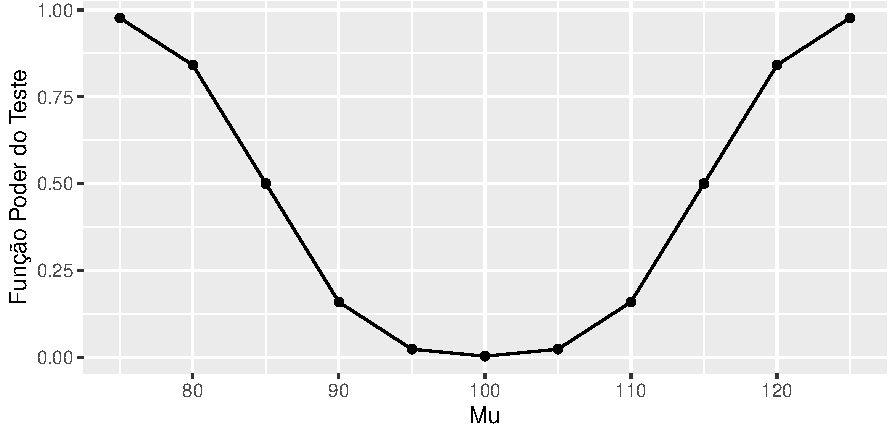
\includegraphics{inferencia_com_R_files/figure-latex/unnamed-chunk-66-1} \end{center}

Observe que, para \(\mu=100\), valor da hipótese nula, a função poder é igual à probabilidade do erro tipo I (nível de significância).

É interessante notar também que quanto mais distante do valor \(\mu_0=100\), maior o poder do teste, ou seja, há uma probabilidade mais alta de se rejeitar \(H_0\) quando o valor alternativo \(\mu\) está bem distante de \(\mu_0\).

Agora, considere a situação do exemplo anterior, com as seguintes diferenças: o tamanho da amostra é \(n=100\) e a região crítica passa a ser

\[RC: \bar X < 94\text{ ou }\bar X > 106\]

Note que é razoável ``estreitar'' a região crítica, já que a amostra é maior. Nesse caso, \(\alpha\) é exatamente igual ao do exemplo anterior, já a função poder do teste para os mesmos valores (em vermelho \(n=100\)):

\begin{center}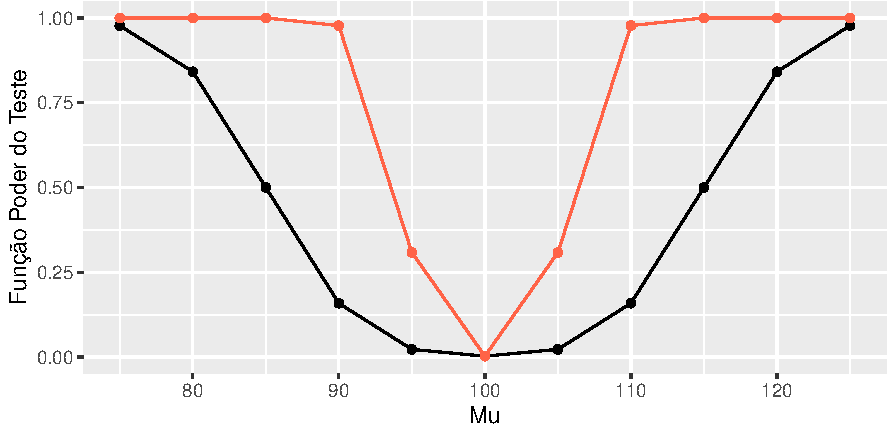
\includegraphics{inferencia_com_R_files/figure-latex/unnamed-chunk-67-1} \end{center}

Note que o poder do teste baseado em uma amostra de tamanho 100 é sempre maior que o poder do teste baseado em uma amostra de tamanho 16.

\hypertarget{t.h.-para-a-muxe9dia-de-uma-normal-com-variuxe2ncia-conhecida}{%
\section{T.H. para a média de uma Normal com variância conhecida}\label{t.h.-para-a-muxe9dia-de-uma-normal-com-variuxe2ncia-conhecida}}

Neste capítulo iremos aplicar os conceitos básicos sobre a teoria de teste de hipóteses a uma situação específica. Nosso interesse estará concentrado na média de uma população normal. Assim como no caso dos intervalos de confiança, iremos iniciar nossos estudos supondo que a variância dessa população seja conhecida. Como já dito, essa situação não é muito comum na prática, mas, em termos didáticos, a apresentação dos conceitos fica simplificada. Entendendo bem a construção de um teste de hipóteses para esse caso particular, a apresentação para as outras situações é bastante semelhante, mudando apenas a distribuição amostral.

\textbf{Contextualizando com um exemplo}

Depois de uma pane geral no sistema de informação de uma empresa, o gerente administrativo deseja saber se houve alteração no tempo de processamento de determinada atividade. Antes da pane, o tempo de processamento podia ser aproximado por uma variável aleatória normal com média de 100 minutos e desvio padrão de 10 minutos. O gerente acredita que a pane não tenha alterado a variabilidade do processo. Uma amostra de 16 tempos de processamento após a pane revela uma média de 105,5 minutos. Ao nível de significância de 5\%, qual é a conclusão sobre a alteração do tempo médio de processamento?

\textbf{Solução}

O interesse do gerente é comparar os tempos antes e depois da pane. Antes da pane, o tempo médio de processamento era de 100 minutos. Como ele não sabe o tipo de alteração que possa ter ocorrido, ele precisa saber se o tempo médio depois da pane é diferente do tempo anterior. Isso nos leva às seguintes hipóteses nula e alternativa:

\[H_0:\mu=100\text{  vs  } H_1:\mu\neq 100\]

Seja \(X\) a variável aleatória que representa o tempo de processamento. Então, pelos dados do problema, temos que \(X\sim N(\mu; 100)\). Antes da pane, \(\mu =100\). Como a população é normal, sabemos que a distribuição da média amostral também é normal e como não deve ter havido alteração na variabilidade do processo, resulta que o desvio padrão é de 10 minutos em qualquer situação. Logo,

\[\bar X \sim N\left(\mu,\frac{100}{16}\right)\]

ou equivalentemente,

\[Z=\frac{\bar X-\mu}{2,5}\sim N(0,1)\]

Pelo enunciado do problema, o nível de significância é de 5\%. Isso significa que a probabilidade do erro tipo I é 0,05. Como visto, o erro tipo I consiste em rejeitar a hipótese nula quando ela é verdadeira. Logo,

\[\alpha=P(\text{rejeitar }H_0|H_0\text{ verdadeira})=0,05\]

Quando \(H_0\) verdadeira, a estatística de teste tem a seguinte distribuição:

\[H_0\text{ verdadeira} \Rightarrow \bar X \sim N\left(100,\frac{100}{16}\right)\]

ou equivalentemente,

\[Z=\frac{\bar X-100}{\sqrt{\frac{100}{16}}}\sim N(0,1)\]

A nossa região crítica consiste nos valores de \(X\) com probabilidade pequena de ocorrerem sob essa hipótese. Ou seja, a região crítica consiste nos valores de \(X\) muito afastados da média suposta de \(\mu=100\). Como a hipótese alternativa é bilateral, ``muito afastado'' significa ``muito maior'' ou ``muito menor'' do que \(\mu=100\).

\begin{center}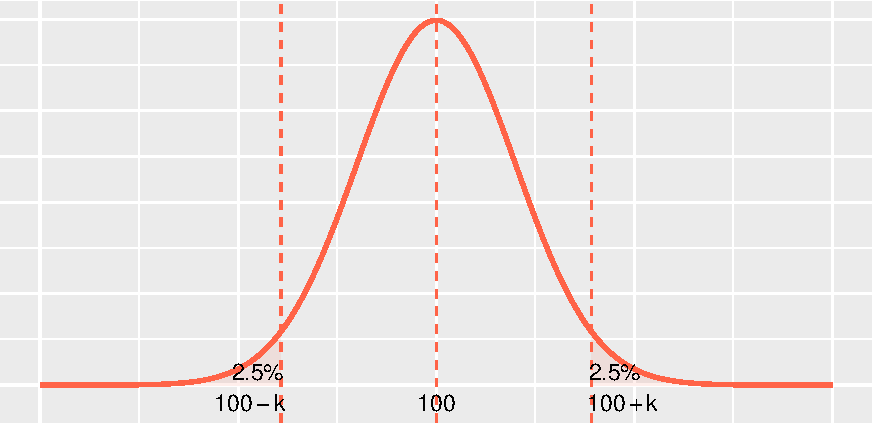
\includegraphics{inferencia_com_R_files/figure-latex/unnamed-chunk-68-1} \end{center}

Então, nossa região crítica é

\[\bar X < 100-k \text{  ou  } \bar X  > 100+k\]

e isso é equivalente a

\[\bar X -100 < -k \text{  ou  } \bar X -100 > +k\]

Usando a função módulo, podemos escrever:

\[RC: |\bar X -100|>k\]

e o valor da constante \(k\) é determinado pelo nível de significância:

\(P\left[|\bar X -100|>k\Big|\bar X \sim N\left(100;6,25\right)\right] = 0,05\)

\(P\left(\bar X < 100-k|\bar X \sim N(100,6,25)\right)+P\left(\bar X > 100+k|\bar X \sim N(100,6,25)\right) = 0,05\)

\(P\left(Z<\frac{-k}{2,5}\right)+P\left(Z>\frac{k}{2,5}\right) = 0,05\)

\(P\left(Z>\frac{k}{2,5}\right)+P\left(Z>\frac{k}{2,5}\right) = 0,05\)

\(P\left(Z>\frac{k}{2,5}\right) = 0,025\)

Como, \(z_{0,025}=1.96\), então \(\frac{k}{2,5}=1,96\), assim \(k=4,9\).

A região crítica é

\[RC: \bar X<95,1\text{  ou  }\bar X>104,9\]

Como o valor da estatística de teste para a amostra observada está na região crítica, devemos rejeitar a hipótese nula, ou seja, as evidências amostrais indicam uma alteração do tempo de processamento da tarefa após a pane.

A função poder do teste é definida como

\[\beta(\mu)=P(\text{rejeitar } H_0|\mu)\]

Em termos da nossa região crítica podemos escrever

\[
\begin{aligned}
\beta(\mu)&= P\left[\bar X<95,1 |\bar X \sim N(100,6,25)\right] + P\left[\bar X>104,9 |\bar X \sim N(100,6,25)\right] \\
&=P\left[Z<\frac{95,1-\mu}{2,5}\right]+P\left[Z>\frac{104,9-\mu}{2,5}\right]
\end{aligned}
\]

Calculando \(\beta(\mu)\) para diferentes valores de \(\mu\) obtemos o gráfico exibido na Figura abaixo:

\begin{center}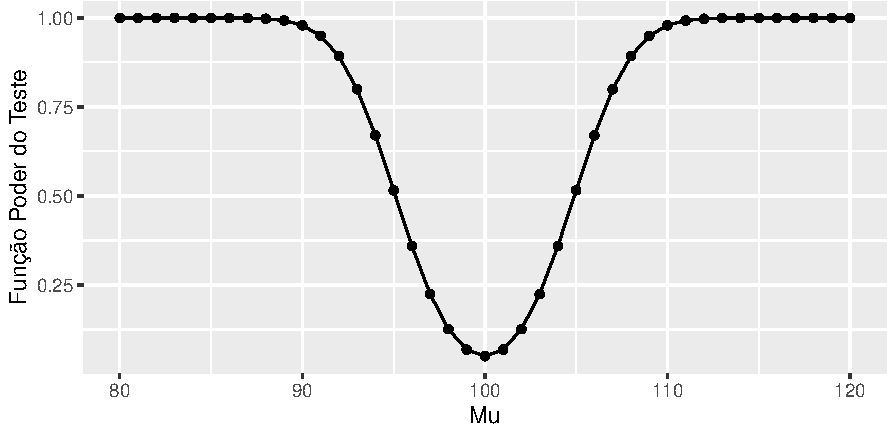
\includegraphics{inferencia_com_R_files/figure-latex/unnamed-chunk-69-1} \end{center}

\hypertarget{construindo-o-teste-de-hipuxf3teses}{%
\subsection{Construindo o teste de hipóteses}\label{construindo-o-teste-de-hipuxf3teses}}

De posse de uma amostra aleatória simples \(X_1, X_2, \ldots, X_n\) extraída de uma população \(X\sim N(\mu; \sigma^2)\), nosso interesse está em testar a hipótese nula

\[H_0: \mu = \mu_0\]

a um nível de significância \(\alpha\).

Dependendo do conhecimento sobre o problema, a hipótese alternativa pode tomar uma das três formas:

\[H_1:\mu\neq\mu_0~~~~~~H_1:\mu>\mu_0~~~~~~H_1:\mu<\mu_0\]

Em qualquer dos casos, a estatística de teste é a média amostral; se a variância \(\sigma^2\) é conhecida, sabemos que

\[\bar X \sim N\left(\mu,\frac{\sigma^2}{n}\right)\]

A regra de decisão consiste em rejeitar a hipótese nula se o valor de \(\bar X\) estiver ``longe'' do valor \(\mu_0\). No caso da hipótese alternativa bilateral, estar longe significa ser muito maior ou muito menor que \(\mu_0\); para a alternativa unilateral à direita, estar longe significa ser muito maior do que \(\mu_0\) e para a alternativa unilateral à esquerda, longe significa ser muito menor que \(\mu_0\). As expressões ``muito menor'' e ``muito maior'' ficam perfeitamente definidas a partir do valor do nível de significância \(\alpha\).

Veja as Figuras abaixo, em que ilustra-se a região crítica para as três hipóteses alternativas. Como antes, vamos denotar por \(z_\alpha\) a abscissa da curva normal padrão que deixa área (probabilidade) \(\alpha\) acima dela.

\begin{center}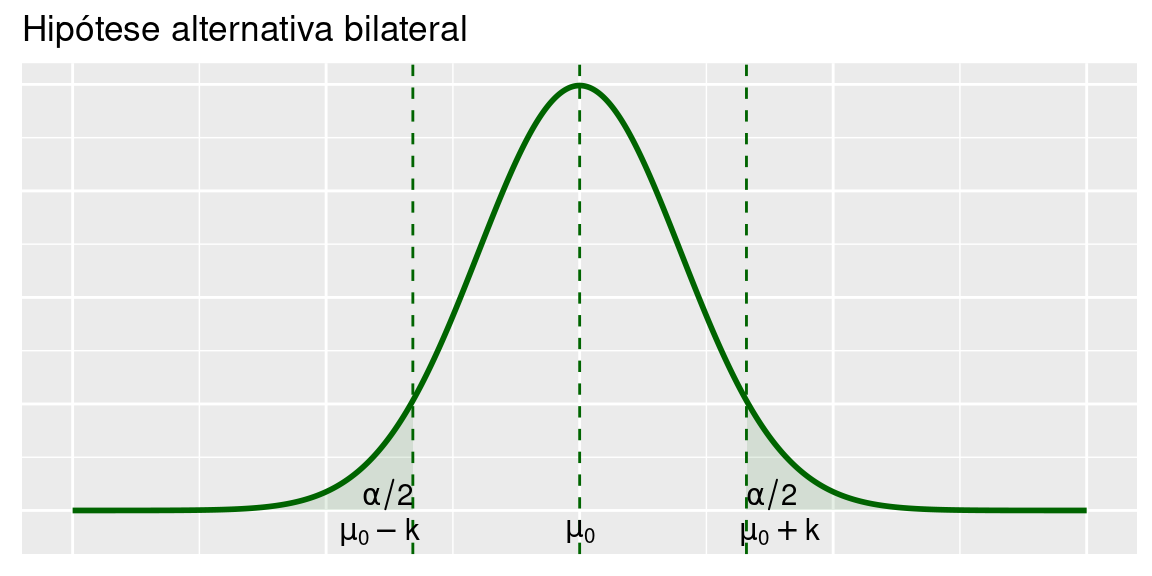
\includegraphics{inferencia_com_R_files/figure-latex/unnamed-chunk-70-1} \end{center}

\begin{center}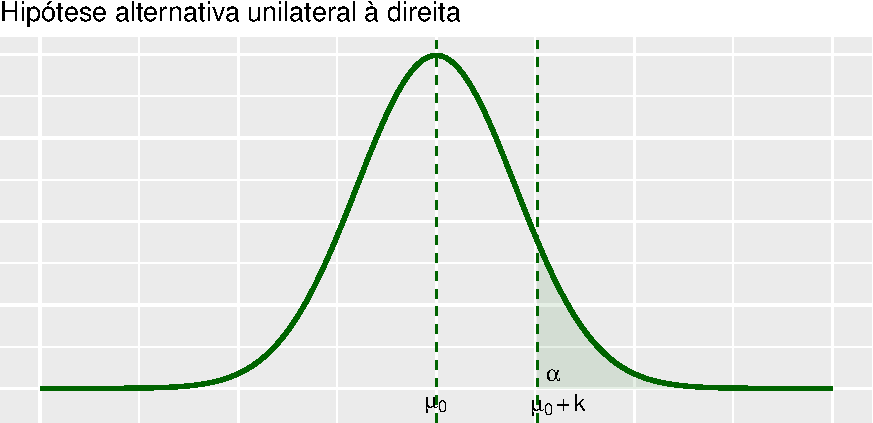
\includegraphics{inferencia_com_R_files/figure-latex/unnamed-chunk-71-1} \end{center}

\begin{center}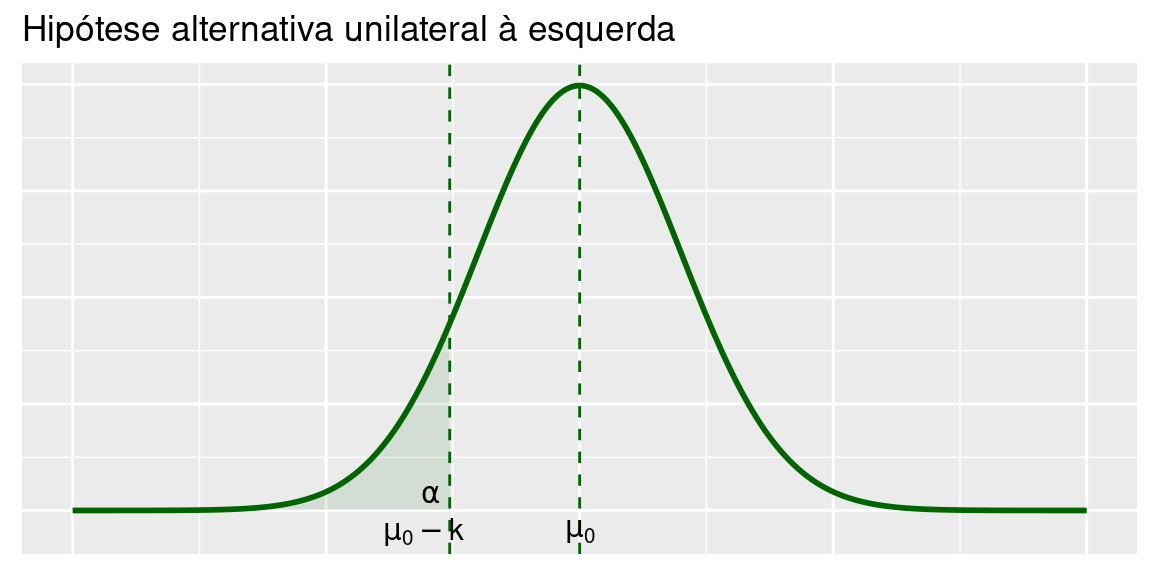
\includegraphics{inferencia_com_R_files/figure-latex/unnamed-chunk-72-1} \end{center}

\hypertarget{bilateral}{%
\subsubsection{Bilateral}\label{bilateral}}

Consideremos as hipóteses

\[H_0:\mu=\mu_0 \text{  vs  } H_1:\mu\ne\mu_0\]

A região crítica é

\[\bar X < \mu_0-k\text{ ou }\bar X > \mu_0+k\]

e se a hipótese nula é verdadeira,

\[\bar X \sim N\left(\mu_0,\frac{\sigma^2}{n}\right)\]

Com nível de significância \(\alpha=P(\text{erro tipo I})\), temos que ter:

\(\alpha=P\left(\text{rejeitar }H_0|H_0\text{ verdadeira}\right)\)

\(\alpha=P\left(\bar X < \mu_0-k\text{ ou }\bar X > \mu_0+k|\bar X \sim N\left(\mu_0,\frac{\sigma^2}{n}\right)\right)\)

\(\alpha=P\left(\bar X < \mu_0-k|\bar X \sim N\left(\mu_0,\frac{\sigma^2}{n}\right)\right) + P\left(\bar X > \mu_0+k|\bar X \sim N\left(\mu_0,\frac{\sigma^2}{n}\right)\right)\)

\(\alpha=P\left(Z<\frac{-k}{\frac{\sigma}{\sqrt n}}\right)+P\left(Z>\frac{k}{\frac{\sigma}{\sqrt n}}\right)\)

\(\alpha=2\times P\left(Z>\frac{k}{\frac{\sigma}{\sqrt n}}\right)\)

\(\frac{\alpha}{2}=P\left(Z>\frac{k}{\frac{\sigma}{\sqrt n}}\right)\)

\(\frac{k}{\frac{\sigma}{\sqrt n}}=z_{\frac{\alpha}{2}}\)

\(k = z_{\frac{\alpha}{2}}\frac{\sigma}{\sqrt n}\)

Logo, a região crítica é:

\[\bar X < \mu_0-z_{\frac{\alpha}{2}}\frac{\sigma}{\sqrt n}\text{ ou }\bar X > \mu_0+z_{\frac{\alpha}{2}}\frac{\sigma}{\sqrt n}\]

\hypertarget{unilateral-uxe0-direita}{%
\subsubsection{Unilateral à direita}\label{unilateral-uxe0-direita}}

Consideremos as hipóteses

\[H_0:\mu=\mu_0 \text{  vs  } H_1:\mu>\mu_0\]

A região crítica é

\[\bar X > \mu_0+k\]

e se a hipótese nula é verdadeira,

\[\bar X \sim N\left(\mu_0,\frac{\sigma^2}{n}\right)\]

Com nível de significância \(\alpha=P(\text{erro tipo I})\), temos que ter:

\(\alpha=P\left(\text{rejeitar }H_0|H_0\text{ verdadeira}\right)\)

\(\alpha=P\left(\bar X > \mu_0+k|\bar X \sim N\left(\mu_0,\frac{\sigma^2}{n}\right)\right)\)

\(\alpha=P\left(Z>\frac{k}{\frac{\sigma}{\sqrt n}}\right)\)

\(\frac{k}{\frac{\sigma}{\sqrt n}}=z_{\alpha}\)

\(k = z_{\alpha}\frac{\sigma}{\sqrt n}\)

Logo, a região crítica é:

\[\bar X > \mu_0+z_{\alpha}\frac{\sigma}{\sqrt n}\]

\hypertarget{unilateral-uxe0-esquerda}{%
\subsubsection{Unilateral à esquerda}\label{unilateral-uxe0-esquerda}}

Consideremos as hipóteses

\[H_0:\mu=\mu_0 \text{  vs  } H_1:\mu<\mu_0\]

A região crítica é

\[\bar X < \mu_0-k\]

e se a hipótese nula é verdadeira,

\[\bar X \sim N\left(\mu_0,\frac{\sigma^2}{n}\right)\]

Com nível de significância \(\alpha=P(\text{erro tipo I})\), temos que ter:

\(\alpha=P\left(\text{rejeitar }H_0|H_0\text{ verdadeira}\right)\)

\(\alpha=P\left(\bar X < \mu_0-k|\bar X \sim N\left(\mu_0,\frac{\sigma^2}{n}\right)\right)\)

\(\alpha=P\left(Z<-\frac{k}{\frac{\sigma}{\sqrt n}}\right)\)

\(\alpha=P\left(Z>\frac{k}{\frac{\sigma}{\sqrt n}}\right)\)

\(\frac{k}{\frac{\sigma}{\sqrt n}}=z_{\alpha}\)

\(k = z_{\alpha}\frac{\sigma}{\sqrt n}\)

Logo, a região crítica é:

\[\bar X < \mu_0-z_{\alpha}\frac{\sigma}{\sqrt n}\]

\hypertarget{teste-de-hipuxf3teses-vs-intervalo-de-confianuxe7a}{%
\subsection{Teste de Hipóteses vs Intervalo de Confiança}\label{teste-de-hipuxf3teses-vs-intervalo-de-confianuxe7a}}

É interessante notar a expressão que aparece na região crítica para o teste bilateral; ela é a mesma obtida para a margem de erro do intervalo de confiança para a média de uma população normal com variância conhecida:

\[\varepsilon=z_{\frac{\alpha}{2}}\frac{\sigma}{\sqrt n}\]

Podemos ver, assim, que existe uma relação entre os dois procedimentos; na verdade, em um teste de hipóteses bilateral, rejeitamos a hipótese nula \(H_0\) se o valor observado da estatística de teste não estiver no intervalo de confiança.

\hypertarget{valor-p-ou-p-valor}{%
\subsection{Valor P (ou p-valor)}\label{valor-p-ou-p-valor}}

Nos exemplos acima, a determinação da região crítica foi feita com base no nível de significância, isto é, fixado o nível de significância encontramos o valor \(k\) que definia os limites entre valores prováveis (aqueles que levam à não rejeição de \(H_0\)) e pouco prováveis (aqueles que levam à rejeição de \(H_0\)). Um outro procedimento bastante usual, especialmente quando são utilizados programas computacionais, consiste em calcular a probabilidade de se obter um valor tão ou mais desfavorável que o valor observado, se \(H_0\) for verdadeira. Essa probabilidade é chamada valor P ou p-valor.

Portanto, definimos p-valor como: a probabilidade de obtermos um valor tão ou mais extremo que o valor observado dado que \(H_0\) é verdadeira. Devemos rejeitar a hipótese nula \(H_0\) ao nível de significância \(\alpha\) sempre que o p-valor for menor ou igual a \(\alpha\),ou seja:

\[\text{Rejeitamos } H_0\Leftrightarrow \text{p-valor} \leq \alpha\]

\hypertarget{exemplo-3}{%
\subsection{Exemplo}\label{exemplo-3}}

\textbf{Solução}

No exemplo exposto no início da seção, o valor obtido com os dados amostrais para a estatística de teste foi \(\bar x = 105,5\). Como o teste é bilateral, valores ``longe'' de 100 são aqueles muito menores ou muito maiores que 100. O procedimento visto consistiu em dividir a probabilidade do erro tipo I igualmente nas duas caudas da distribuição normal e dessa forma identificamos a região crítica. Vamos, agora, calcular o valor P para o nosso exemplo; ele é a probabilidade de obtermos um valor tão ou mais extremo que o valor observado. Como o valor observado está à direita da média, devemos calcular a seguinte probabilidade:

\[
\begin{aligned}
P &= P\left(\bar X \geq 105,5|H_0\text{ verdadeira}\right)\\
&= P\left[\bar X \geq 105,5|\bar X \sim N\left(100;\frac{100}{16}\right)\right]\\
&=P\left(Z\geq \frac{105,5-100}{2,5}\right)\\
&=P(Z\geq 2,2)\\
&=0,0139
\end{aligned}
\]

Vamos analisar a Figura abaixo, onde está ilustrado esse valor. O valor amostral observado para \(\bar X\) é \(\bar x = 105,5 = 100+5,5\). Como o teste é bilateral, se tivéssemos obtido o valor \(\bar x = 100 - 5,5\), esse valor também seria considerado tão afastado de \(100\) quanto \(105,5\). Assim, para testes bilaterais, temos que considerar a probabilidade nas duas caudas da distribuição. O que esse resultado está nos dizendo é o seguinte: se \(H_0\) for verdadeira, a probabilidade de obtermos um valor distante de \(100\) por \(5,5\) unidades em qualquer direção é \(2\times 0,0139 = 0,0278\). Essa probabilidade é chamada valor P.

\begin{center}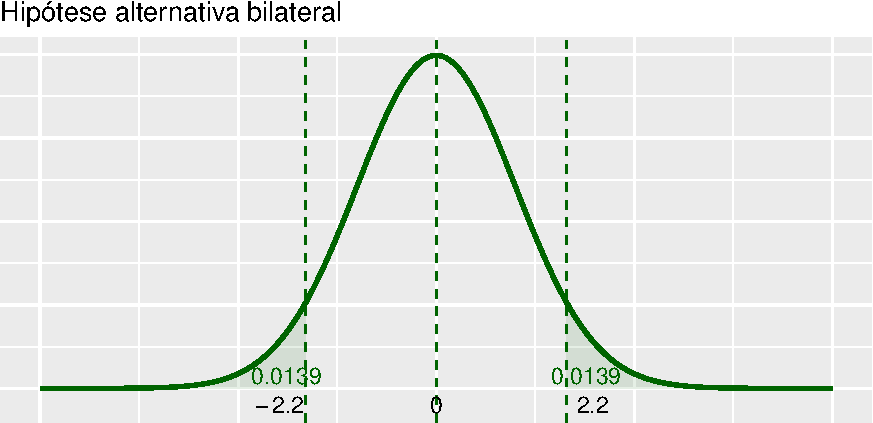
\includegraphics{inferencia_com_R_files/figure-latex/unnamed-chunk-73-1} \end{center}

No exemplo, vemos que o valor P é pequeno, o que significa que é pouco provável obtermos um valor tão extremo quando \(H_0\) é verdadeira. Logo, é razoável supormos que a hipótese nula não seja verdadeira, a mesma conclusão obtida ao trabalharmos com o nível de significância de 5\%. Na verdade, rejeitaríamos a hipótese nula para qualquer nível de significância maior que \(0,0278\).

\hypertarget{t.h.-para-a-muxe9dia-de-uma-normal-com-variuxe2ncia-desconhecida}{%
\section{T.H. para a média de uma Normal com variância desconhecida}\label{t.h.-para-a-muxe9dia-de-uma-normal-com-variuxe2ncia-desconhecida}}

Neste capítulo você completará seu estudo básico de testes de hipóteses sobre a média de uma população, analisando a situação relativa a uma população normal quando não se conhece a variância desta população. Assim como no caso do intervalo de confiança, para testar hipóteses relativas à média de tal população, é necessário estimar essa variância e isso introduz mais uma fonte de variabilidade no procedimento: com uma única amostra, queremos testar hipóteses sobre a média, mas precisamos também estimar a variância da população. O procedimento é simples e análogo aos casos estudados nos caítulos anteriores; o que muda é a distribuição amostral da estatística de teste. Em vez de usarmos a distribuição normal para determinar os valores críticos, usaremos novamente a distribuição t de Student.

Considere uma população descrita por uma variável aleatória normal com média \(\mu\) e variância \(\sigma^2\): \(X\sim N(\mu,\sigma^2)\). Nosso interesse é testar hipóteses sobre a média \(\mu\) a partir de uma amostra aleatória simples \(X_1, X_2, \ldots, X_n\). Como visto anteriormente, se a variância \(\sigma^2\) não é conhecida, então temos que usar a estatística

\[T=\sqrt{n}\frac{\bar X-\mu}{S}\]

cuja distribuição \(t\) de Student com \(n-1\) graus de liberdade.

\hypertarget{construindo-o-teste-de-hipuxf3teses-1}{%
\subsection{Construindo o teste de hipóteses}\label{construindo-o-teste-de-hipuxf3teses-1}}

De posse desta estatística de teste, o procedimento de construção do teste é idêntico ao visto anteriormente: identificadas a hipótese nula (sempre na forma de uma hipótese simples \(\mu=\mu_0\)) e a hipótese alternativa, a região crítica é formada pelos valores da estatística de teste pouco prováveis sob \(H_0\). O nível de significância e o tipo de hipótese alternativa permitem a identificação precisa do que são ``valores pouco prováveis'': são valores na(s) cauda(s) da distribuição de \(T\) quando a hipótese nula é verdadeira.

Seja \(X_1,X_2,\ldots,X_n\) uma amostra amostra aleatória simples de uma população \(X\) cuja disribuição é \(N(\mu; \sigma^2)\). Nosso interesse é testar alguma hipótese sobre a média \(\mu\) desta população. Em geral, a variância \(\sigma^2\) não é conhecida e, portanto, vamos estimá-la por

\[S^2=\frac{1}{n-1}\sum_{i=1}^n \left(X_i-\bar X\right)^2\]

Lembre-se que \(S^2\) é um estimador não-viesado de \(\sigma^2\).

A hipótese nula que iremos considerar será

\[H_0:\mu=\mu_0\]

As possíveis formas da hipótese alternativa são:

\begin{itemize}
\tightlist
\item
  Bilateral: \(H_1:\mu\ne\mu_0\)
\item
  Unilateral à direita: \(H_1:\mu > \mu_0\)
\item
  Unilateral à esuqerda: \(H_1:\mu < \mu_0\)
\end{itemize}

Como antes, a escolha entre essas três possibilidades se faz com base no conhecimento do problema. Se não temos informação alguma sobre a alternativa, temos que usar um teste bilateral.

Como o teste é sobre a média de uma população normal, a estatística amostral que deve ser utilizada é \(\bar X\). Como a variância populacional não é conhecida, sabemos que

\[T=\frac{\bar X-\mu}{\frac{S}{\sqrt n}} \sim t(n-1)\]

e é a nossa estatística de teste.

A regra de decisão consiste em definir a região crítica RC como o conjunto de valores cuja probabilidade de ocorrência é pequena sob a hipótese de veracidade de \(H_0\). Logo, nossa regra de decisão se baseia na estatística de teste

\[T_0=\frac{\bar X-\mu_0}{\frac{S}{\sqrt n}} \sim t(n-1)\]

Como a estatística de teste segue uma distribuição t de Student, valores com pequena probabilidade de ocorrência estão nas caudas da distribuição. Isso equivale a valores de \(\bar X\) ``distandes'' de \(\mu_0\). Assim, a região crítica para cada tipo de hipótese alternativa é definida como segue:

\begin{itemize}
\tightlist
\item
  Bilateral: \(T_0 < -k\) ou \(T_0 > k\)
\item
  Unilateral à direita: \(T_0 > k\)
\item
  Unilateral à esuqerda: \(T_0 < -k\)
\end{itemize}

Nas Figuras abaixo ilustram-se as regiões críticas para cada tipo de hipótese alternativa.

\begin{center}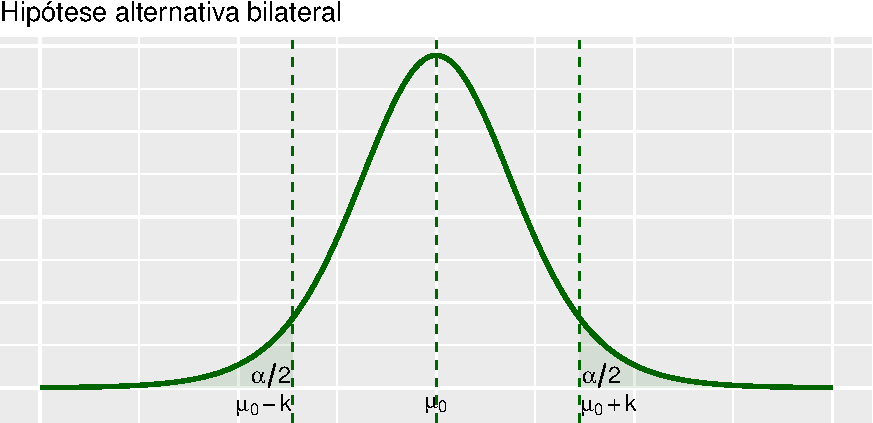
\includegraphics{inferencia_com_R_files/figure-latex/unnamed-chunk-74-1} \end{center}

\begin{center}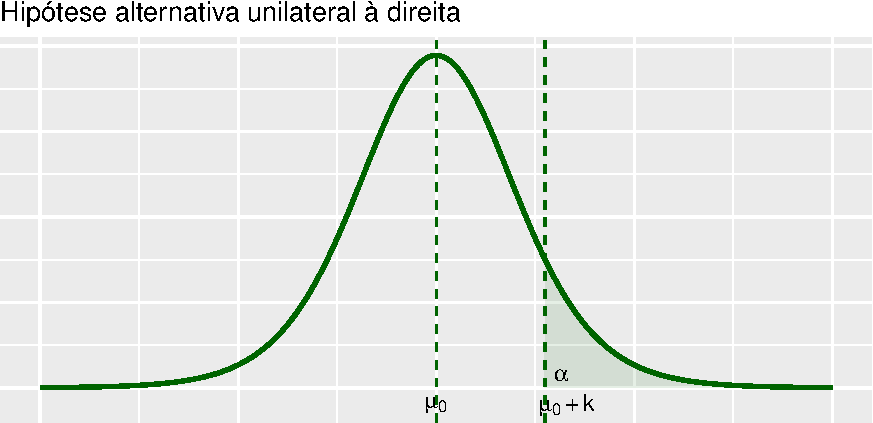
\includegraphics{inferencia_com_R_files/figure-latex/unnamed-chunk-75-1} \end{center}

\begin{center}\includegraphics{inferencia_com_R_files/figure-latex/unnamed-chunk-76-1} \end{center}

O procedimento usual de teste de hipóteses consiste em se fixar o nível de significância \(\alpha\), que, por definição, é a probabilidade de se cometer o erro tipo I:

\[\alpha = P(\text{erro tipo I}) = P(\text{rejeitar }H_0|H_0\text{ é verdadeira})\]

Assim, para cada tipo de hipótese alternativa a região crítica é identificada impondo-se a condição \(P(T \in RC|H0\text{ é verdadeira}) = \alpha\)

\hypertarget{bilateral-1}{%
\subsubsection{Bilateral}\label{bilateral-1}}

A região crítica é calculada como:

\[
\begin{aligned}
\alpha&=P\left[T_0<-k\right|T_0\sim t(n-1)]+P\left[T_0>k\right|T_0\sim t(n-1)]\\
\alpha&=2\times P\left[T_0<-k\right|T_0\sim t(n-1)]\\
\frac{\alpha}{2}&=P\left[T_0>k\right|T_0\sim t(n-1)]
\end{aligned}
\]

Usando a notação \(t_{n;\alpha}\) para denotar a abcissa da distribuição \(t\) de Student com \(n\) graus de liberdade que deixa área (probabilidade) \(\alpha\) acima dela, resulta a seguinte região crítica para o teste bilateral:

\[T_0<-t_{n-1;\frac{\alpha}{2}}~~~~~~\text{ou}~~~~~~T_0>t_{n-1;\frac{\alpha}{2}}\]

Essa região crítica também pode ser escrita de outra forma usando a seguinte equivalência:

\[T_0<-t_{n-1;\frac{\alpha}{2}}\Longrightarrow \frac{\bar X-\mu_0}{\frac{S}{\sqrt n}}<-t_{n-1;\frac{\alpha}{2}}\Longrightarrow\bar X<\mu_0-t_{n-1;\frac{\alpha}{2}}\frac{S}{\sqrt n}\]

\[T_0>t_{n-1;\frac{\alpha}{2}}\Longrightarrow \frac{\bar X-\mu_0}{\frac{S}{\sqrt n}}>t_{n-1;\frac{\alpha}{2}}\Longrightarrow\bar X>\mu_0+t_{n-1;\frac{\alpha}{2}}\frac{S}{\sqrt n}\]

\hypertarget{unilateral-uxe0-direita-1}{%
\subsubsection{Unilateral à direita}\label{unilateral-uxe0-direita-1}}

A região crítica é calculada como:

\[
\begin{aligned}
\alpha&=P\left[T_0>k\right|T_0\sim t(n-1)]\\
t_{n-1;\alpha}&=k
\end{aligned}
\]

ou seja, a região crítica é

\[T_0 > t_{n-1;\alpha}\]

ou equivalentemente

\[\bar X>\mu_0+t_{n-1;\alpha}\frac{S}{\sqrt n}\]

\hypertarget{unilateral-uxe0-esquerda-1}{%
\subsubsection{Unilateral à esquerda}\label{unilateral-uxe0-esquerda-1}}

De forma análoga, obtém-se a seguinte região crítica para o teste unilateral à esquerda:

\[T_0 <- t_{n-1;\alpha}\]

ou equivalentemente

\[\bar X<\mu_0-t_{n-1;\alpha}\frac{S}{\sqrt n}\]
\#\#\# Teste de Hipóteses vs Intervalo de Confiança

xxx

\hypertarget{valor-p-ou-p-valor-1}{%
\subsection{Valor P (ou p-valor)}\label{valor-p-ou-p-valor-1}}

XXX

\hypertarget{exemplo-4}{%
\subsection{Exemplo}\label{exemplo-4}}

Depois de uma pane geral no sistema de informação de uma empresa, o gerente administrativo deseja saber se houve alteração no tempo de processamento de determinada atividade. Antes da pane, o tempo de processamento podia ser aproximado por uma variável aleatória normal com média de 100 minutos. Uma amostra de 16 tempos de processamento após a pane revela uma média \(\bar x = 105,5\) minutos e um desvio padrão \(s = 10\) minutos. Ao nível de significância de 5\%, qual é a conclusão sobre a alteração do tempo médio de processamento?

\textbf{Solução}

Como visto, as hipóteses do problema são:

\[
\begin{cases}
H_0:\mu=\mu_0 \\
H_1:\mu\ne\mu_0
\end{cases}
\]

Como a variância não é conhecida, temos que usar a distribuição \(t\) de Student com \(n-1=16-1=15\) graus de liberdade. Para um teste bilateral com nível de significância de 5\%, a abscissa de interesse é aquela que deixa área de \(0,025\) acima. Consultando a Tabela, resulta

\[t_{15;0,025}=2,131\]

A estatística de teste é

\[T_0=\frac{\bar X -100}{\frac{10}{\sqrt{16}}}\sim t(15)\]

e a região crítica é

\[T_0<-2,131~~~~\text{ou}~~~~T_0>2,131\]

O valor observado da estatísitca de teste é

\[T_0=\frac{105,5 -100}{\frac{10}{\sqrt{16}}}=2,2\]

Como esse valor pertence à região crítica, rejeitamos a hipótese nula e concluímos que houve alteração no tempo de processamento após a pane.

Em termos da média amostral, a região crítica é

\[\bar X<100-2,131\times\frac{10}{\sqrt{16}}~~~~\text{ou}~~~~\bar X>100+2,131\times\frac{10}{\sqrt{16}}\]

ou

\[\bar X<105,33~~~~\text{ou}~~~~\bar X>94,673\]

Comparando com a Região Crítica obtida no Exemplo 1 da seção anterior (\(\bar X < 95.1\text{ ou }\bar X > 104.9\)), note que com o mesmo nível de significância, a região crítica no caso de variância desconhecida é mais extrema, refletindo a maior variabilidade da distribuição t-student.

\begin{center}\includegraphics{inferencia_com_R_files/figure-latex/unnamed-chunk-77-1} \end{center}

Para calcular o p-valor:

\[
\begin{aligned}
p-valor &= 2\times P\left(\bar X>105,5 \Big| \frac{\bar X-100}{\frac{10}{\sqrt 16}} \sim t(15)\right)\\
&= 2\times P\left(t(15)>\frac{105,5-100}{\frac{10}{\sqrt 16}}\right)\\
&= 2\times P\left(t(15)>2,2\right)\\
&= 2\times 0, 02195 = 0, 0439
\end{aligned}
\]

Como \(p-valor < 0,05\), rejeitamos \(H_0\) ao nível de significância de 5\%.

\hypertarget{t.h.-para-a-proporuxe7uxe3o-populacional}{%
\section{T.H. para a proporção populacional}\label{t.h.-para-a-proporuxe7uxe3o-populacional}}

Já aprendemos a construir testes de hipóteses sobre a média de uma população normal com variância \(\sigma^2\) conhecida. O procedimento baseou-se na distribuição amostral da média amostral que, com as hipóteses de normalidade e conhecimento da variância populacional, sabemos ser normal com a mesma média e variância \(\frac{\sigma^2}{n}\). Agora, iremos fazer uso do Teorema Limite Central para construir testes de hipóteses sobre proporções com base em amostras grandes. Vimos que, para amostras grandes, a distribuição amostral da proporção amostral pode ser aproximada por uma distribuição normal e, assim, o procedimento de teste de hipóteses será idêntico ao estudado sobre a média de uma população normal com variância \(\sigma^2\) conhecida.

O contexto de interesse é o seguinte: temos uma população em que cada elemento é classificado de acordo com a presença ou ausência de determinada característica. Em termos de variável aleatória, essa população é representada por uma v.a. de Bernoulli, isto é:

\[
X=\begin{cases}
1,\text{  se elemento possui característica de interesse}\\
0,\text{  se elemento não possui característica de interesse}
\end{cases}
\]

Então, \(P(X = 1) = p\), \(E(X) = p\) e \(V(X) = p(1-p)\). O parâmetro \(p\) é também a proporção de elementos da população que possuem a caracterísitca de interesse. Em geral, esse parâmetro é desconhecido e queremos testar hipóteses feitas sobre seu possível valor.

Suponha, então, que dessa população seja extraída uma amostra aleatória simples \(X_1,\ldots,X_n\) com reposição. Vimos que a proporção \(\hat P\) de elementos na amostra que possuem a característica de interesse, definida por

\[\hat P = \frac{S_n}{n} = \frac{X_1+X_2+\ldots+X_n}{n}\]

é um estimador não-viesado para \(p\) com variância \(\frac{p(1-p)}{n}\). Mais precisamente,

\[E(\hat P)=p\]

\[V(\hat P)=\frac{p(1-p)}{n}\]

\hypertarget{construindo-o-teste-de-hipuxf3teses-2}{%
\subsection{Construindo o teste de hipóteses}\label{construindo-o-teste-de-hipuxf3teses-2}}

Como a proporção amostral é uma média de uma amostra aleatória simples de uma população com distribuição de Bernoulli com parâmetro \(p\), o Teorema Central do Limite nos diz, então, que a distribuição de \(\hat P\) se aproxima de uma nornal com média \(p\) e variância \(\frac{p(1-p)}{n}\).

Resumindo, temos o seguinte resultado:

\[\hat P \approx N\left(p,\frac{p(1-p)}{n}\right)\]

ou, equivalentemente,

\[\frac{\hat P-p}{\sqrt{\frac{p(1-p)}{n}}}\approx N(0,1)\]

Vamos ver, agora, como usar esse resultado para construir testes de hipóteses sobre a verdadeira proporção populacional \(p\).

A hipótese nula que consideraremos será uma hipótese simples:

\[H_0:p=p_0\]

As hipóteses alternativas possíveis são

\begin{itemize}
\tightlist
\item
  Bilateral: \(H_1:p\neq p_0\)
\item
  Unilateral à direita: \(H_1:p > p_0\)
\item
  Unilateral à esquerda: \(H_1:p < p_0\)
\end{itemize}

Como no caso da média, a escolha das hipóteses nula e alternativa deve ser feita levando-se em conta que a hipótese nula deve ser uma hipótese simples. Assim, você deve ``traduzir'' a situação de interesse do problema em desigualdades envolvendo a proporção \(p\). A hipótese alternativa é a desigualdade que não inclui o sinal de \(=\). A estatística de teste é

\[Z=\frac{\hat P-p}{\sqrt{\frac{p(1-p)}{n}}}\approx N(0,1)\]

Dado um nível de significância \(\alpha\), a região crítica é definida como o conjunto de valores da estatísttca de teste que têm probabilidade pequena de ocorrerem sob a veracidade da hipótese nula. Assim, a região crítica é definida como o conjunto de valores de

\[Z_0=\frac{\hat P-p_0}{\sqrt{\frac{p_0(1-p_0)}{n}}}\approx N(0,1)\]

com pequena probabilidade de ocorrência. Como estamos exatamente no mesmo procedimento de teste de hipóteses será idêntico ao estudado sobre a média de uma população normal com variância \(\sigma^2\) conhecida,

\begin{itemize}
\tightlist
\item
  \(Z_0 < -Z_\frac{\alpha}{2}\) ou \(Z_0>Z_\frac{\alpha}{2}\) (teste bilateral)
\item
  \(Z_0 > z_\alpha\) (teste unilateral à direita)
\item
  \(Z_0 < -z_\alpha\) (teste unilateral à esquerda)
\end{itemize}

ou

\begin{itemize}
\tightlist
\item
  \(\hat P < p_0-Z_\frac{\alpha}{2}\sqrt{\frac{p_0(1-p_0)}{n}}\) ou \(\hat P > p_0+Z_\frac{\alpha}{2}\sqrt{\frac{p_0(1-p_0)}{n}}\) (teste bilateral)
\item
  \(\hat P > p_0+Z_\alpha\sqrt{\frac{p_0(1-p_0)}{n}}\) (teste unilateral à direita)
\item
  \(\hat P < p_0-Z_\alpha\sqrt{\frac{p_0(1-p_0)}{n}}\) (teste unilateral à direita)
\end{itemize}

\hypertarget{valor-p-ou-p-valor-2}{%
\subsection{Valor P (ou p-valor)}\label{valor-p-ou-p-valor-2}}

Como já visto, o valor P é a probabilidade de se obter um valor tão ou mais extremo (na direção da hipótese alternativa) que o valor observado da estatística de teste. Denotando por \(Z_0\) o valor observado da estatística de teste, temos as seguintes possibilidades:

\begin{itemize}
\tightlist
\item
  \(\text{p-valor}=2\times P(Z>|Z_0|)\) (teste bilateral)
\item
  \(\text{p-valor}= P(Z>|Z_0|)\) (teste unilateral à direita ou à esquerda)
\end{itemize}

Valores pequenos de \(\text{p-valor}\) indicam que o valor observado é pouco provável de ocorrer sob a hipótese nula; logo, valores pequenos de \(\text{p-valor}\) levam à rejeição da hipótese nula. A hipótese nula é rejeitada a qualquer nível de significância \(\alpha \geq \text{p-valor}\).

\hypertarget{exemplo-5}{%
\subsection{Exemplo}\label{exemplo-5}}

Uma amostra de 64 elementos é usada para testar

\[
\begin{cases}
H_0:p=0,35 \\
H_1:p\neq 0,35
\end{cases}
\]

Estabeleça a região crítica para o nível de significância de 1\%. Se a proporção amostral para esta amostra é \(\hat P = 0,26\), calcule o \(\text{p-valor}\).

\textbf{Solução}

Com \(\alpha=0,01\) e um teste bilateral, resulta que \(z_{0,005}=2,59\). A estatística de teste é

\[Z_0=\frac{0,26-0,35}{\sqrt{\frac{0,35\times 0,65}{64}}}=-1,51\]

e a região crítica é

\[Z_0<-2,59~~~~\text{ou}~~~~Z_0>2,59\]

Como o teste é bilateral, o \(\text{p-valor}\) é calculado como

\[
\begin{aligned}
\text{p-valor} &= 2\times P(Z>|-1,51|) \\
&= 2\times 0,0655\\
&= 0,131
\end{aligned}
\]

Como o \(\text{p-valor}\) é grande, não se rejeita a hipótese nula, ou seja, a probabilidade de se obter um valor tão extremo quanto o observado é alta, se \(H_0\) for verdadeira. A hipótese nula só seria rejeitada para níveis de significância maiores que 13,1\%.

\hypertarget{t.h.-para-a-variuxe2ncia-de-uma-normal}{%
\section{T.H. para a variância de uma Normal}\label{t.h.-para-a-variuxe2ncia-de-uma-normal}}

Agora completaremos o estudo de teste de hipóteses sobre parâmetros de uma população, analisando o caso da variância de uma população normal. Assim como na construção de intervalos de confiança, nossa estatística de teste tem distribuição qui-quadrado e a região crítica, como antes, será formada pelos valores pouco prováveis desta estatística de teste sob a hipótese nula.

Considere uma população descrita por uma variável aleatória normal com média \(\mu\) e variância \(\sigma^2: X\sim N(\mu; \sigma^2)\). Nosso interesse é testar hipóteses sobre a a variância \(\sigma^2\) a partir de uma amostra aleatória simples \(X_1, X_2,\ldots, X_n\). Como visto anteriormente, a estatística

\[\chi^2=\frac{(n-1)S^2}{\sigma^2}\]

tem distribuição qui-quadrado com \(n-1\) graus de liberdade.

De posse desta estatística de teste, o procedimento de construção do teste é idêntico ao visto nos últimos capítulos: identificadas a hipótese nula (sempre na forma de uma hipótese simples \(\sigma^2=\sigma^2_0\)) e a hipótese alternativa, a região crítica é formada pelos valores da estatística de teste pouco prováveis sob \(H_0\). O nível de significância e o tipo de hipótese alternativa permitem a identificação precisa do que são ``valores pouco prováveis'': são valores na(s) cauda(s) da distribuição de \(\chi^2\) quando a hipótese nula é verdadeira.

\hypertarget{construindo-o-teste-de-hipuxf3teses-3}{%
\subsection{Construindo o teste de hipóteses}\label{construindo-o-teste-de-hipuxf3teses-3}}

Seja \(X_1, X_2,\ldots, X_n\) uma amostra aleatória simples de uma população \(X\) cuja distribuição é \(N(\mu,\sigma^2)\). Nosso interesse é testar alguma hipótese sobre a variância \(\sigma^2\), que é estimada por

\[S^2=\frac{1}{n-1}\sum_{i=1}^n(X_i-\bar X)^2\]

Lembre-se que \(S^2\) é um estimador não-viesado de \(\sigma^2\).

A hipótese nula que iremos considerar será

\[H_0:\sigma^2=\sigma^2_0\]

As possíveis formas da hipótese alternativa são:

\begin{itemize}
\tightlist
\item
  Bilateral: \(H_1:\sigma^2\neq \sigma^2_0\)
\item
  Unilateral à direita: \(H_1:\sigma^2 > \sigma^2_0\)
\item
  Unilateral à esquerda: \(H_1:\sigma^2 < \sigma^2_0\)
\end{itemize}

Como o teste é sobre a variância de uma população normal, a estatística amostral a ser utilizada é

\[\frac{(n-1)S^2}{\sigma^2}\sim \chi^2_{n-1}\]

O procedimento de decisão é definido em termos da hipótese nula \(H_0\) e as decisões possíveis são (i) rejeitar ou (ii) não rejeitar \(H_0\). Conforme já visto, existem duas possibilidades de erro:

\begin{itemize}
\tightlist
\item
  Erro tipo I: rejeitar \(H_0\) quando \(H_0\) é verdadeira
\item
  Erro tipo II: não rejeitar \(H_0\) quando \(H_0\) é falsa
\end{itemize}

A regra de decisão consiste em definir a região crítica RC como o conjunto de valores cuja probabilidade de ocorrência é pequena sob a hipótese de veracidade de \(H_0\). Logo, nossa regra de decisão se baseia na estatística de teste

\[X_0=\frac{(n-1)S^2}{\sigma^2_0}\sim \chi^2_{n-1}\]

Os valores com pequena probabilidade de ocorrência estão nas caudas da distribuição. Assim, a região crítica para cada tipo de hipótese alternativa é definida como segue:

\begin{itemize}
\tightlist
\item
  \(X_0<k_I\) ou \(X^2_0>k_S\) (teste bilateral)
\item
  \(X_0>k_S\) (teste unilateral à direita)
\item
  \(X_0<k_I\) (teste unilateral à esquerda)
\end{itemize}

\hypertarget{bilateral-2}{%
\subsubsection{Bilateral}\label{bilateral-2}}

O procedimento usual de teste de hipóteses consiste em se fixar o nível de significância \(\alpha\), que, por definição, é a probabilidade do erro tipo I:

\[\alpha=P(\text{erro tipo I})=(\text{rejeitar }H_0|H_0~\text{é verdadeira})\]

Assim, para cada tipo de hipótese alternativa a região crítica é identificada impondo-se a condição

\[P(X_0 \in RC|H_0~\text{é verdadeira})=\alpha\]

A região crítica é calculada como:

\[P\left[X_0<k_I|X_0\sim\chi^2_{n-1}\right]+P\left[X_0>k_S|X_0\sim\chi^2_{n-1}\right]=\alpha\]

Mesmo a distribuição qui-quadrado não sendo simétrica, é prática usual dividir a probabilidade de erro em partes iguais, ou seja, os limites da região crítica são definidos de modo que

\begin{itemize}
\tightlist
\item
  \(P\left[X_0<k_I|X_0\sim\chi^2_{n-1}\right]=\frac{\alpha}{2}\)
\item
  \(P\left[X_0>k_S|X_0\sim\chi^2_{n-1}\right]=\frac{\alpha}{2}\)
\end{itemize}

\begin{center}\includegraphics{inferencia_com_R_files/figure-latex/unnamed-chunk-78-1} \end{center}

Usando a notação \(\chi^2_{n,\alpha}\) para denotar a abscissa da distribuição qui-quadrado com \(n\) graus de liberdade que deixa área (probabilidade) \(\alpha\) acima dela, resulta a seguinte região crítica para o teste bilateral:

\[X_0<\chi^2_{n-1,1-\frac{\alpha}{2}}~~~~\text{ou}~~~~X_0>\chi^2_{n-1,\frac{\alpha}{2}}\]

ou também,

\[S^2<\frac{n-1}{\sigma^2_0}\chi^2_{n-1,1-\frac{\alpha}{2}}~~~~\text{ou}~~~~S^2>\frac{n-1}{\sigma^2_0}\chi^2_{n-1,\frac{\alpha}{2}}\]

\hypertarget{unilateral-uxe0-direita-2}{%
\subsubsection{Unilateral à direita}\label{unilateral-uxe0-direita-2}}

A região crítica é calculada como:

\[P\left[X_0>k_S|X_0\sim\chi^2_{n-1}\right]=\alpha\Longrightarrow k_S=\chi^2_{n-1,\alpha}\]

ou seja, a região crítica é

\[X_0>\chi^2_{n-1,\alpha}\]

ou também,

\[S^2>\frac{n-1}{\sigma^2_0}\chi^2_{n-1,\alpha}\].

\begin{center}\includegraphics{inferencia_com_R_files/figure-latex/unnamed-chunk-79-1} \end{center}

\hypertarget{unilateral-uxe0-esquerda-2}{%
\subsubsection{Unilateral à esquerda}\label{unilateral-uxe0-esquerda-2}}

De forma análoga, obtém-se a seguinte região crítica para o teste unilateral à esquerda:

\[X_0<\chi^2_{n-1,1-\alpha}\]

ou também,

\[S^2<\frac{n-1}{\sigma^2_0}\chi^2_{n-1,1-\alpha}\].

\begin{center}\includegraphics{inferencia_com_R_files/figure-latex/unnamed-chunk-80-1} \end{center}

\hypertarget{valor-p}{%
\subsection{Valor P}\label{valor-p}}

Como já visto, o valor P é a probabilidade de se obter um valor tão ou mais extremo (na direção da hipótese alternativa) que o valor observado da estatística de teste. Denotando por \(X_0\) o valor observado da estatística de teste, temos as seguintes possibilidades:

\begin{itemize}
\tightlist
\item
  \(\text{p-valor}=2\times \text{mín}\{P(\chi_{n-1}>X_0),P(\chi_{n-1}<X_0)\}\) (teste bilateral)
\item
  \(\text{p-valor}= P(\chi_{n-1}>X_0)\) (teste unilateral à direita)
\item
  \(\text{p-valor}= P(\chi_{n-1}<X_0)\) (teste unilateral à esquerda)
\end{itemize}

Valores pequenos de \(\text{p-valor}\) indicam que o valor observado é pouco provável de ocorrer sob a hipótese nula; logo, valores pequenos de \(\text{p-valor}\) levam à rejeição da hipótese nula. A hipótese nula é rejeitada a qualquer nível de significância \(\alpha \geq \text{p-valor}\).

\hypertarget{exemplo-6}{%
\subsection{Exemplo}\label{exemplo-6}}

XXX

\hypertarget{t.h.-adequauxe7uxe3o-de-ajuste-goodness-of-fit}{%
\section{T.H. Adequação de Ajuste (Goodness of Fit)}\label{t.h.-adequauxe7uxe3o-de-ajuste-goodness-of-fit}}

Os procedimentos de testes de hipóteses que discutimos nas seções prévias são projetados para problemas em que a população ou a distribuição de probabilidades seja conhecida e as hipóteses envolvam os parâmetros da distribuição.

Outro tipo de hipótese é frequentemente encontrada: \emph{Não conhecemos a distribuição sob consideração da população e desejamos testar a hipótese de que uma distribuição particular será satisfatória como um modelo para a população}

Por exemplo, podemos desejar testar a hipótese de que a população seja normal. Ou seja, as hipóteses são:

\[
\begin{cases}
H_0:~~\text{a forma da distribuição da população é (Normal, Poisson etc.)}\\
H_1:~~\text{a forma da distribuição da população não é (Normal, Poisson etc.)}
\end{cases}
\]

Utilizaremos aqui o \textbf{teste de adequação de ajuste}, baseado na distribuição qui-quadrado.

O procedimento de teste requer uma amostra de tamanho \(n\), proveniente da população cuja distribuição de probabilidades é desconhecida. Essas \(n\) observações são arranjadas em um histograma de frequências, tendo \(k\) intervalos de classe onde \(O_i\) é a frequência observada no \(i\)-ésimo intervalo de classe. A partir da distribuição de probabilidades utilizada na hipótese, calculamos a frequência esperada no \(i\)-ésimo intervalo de classe, denotada como \(E_i\).

\hypertarget{construindo-o-teste-de-hipuxf3teses-4}{%
\subsection{Construindo o teste de hipóteses}\label{construindo-o-teste-de-hipuxf3teses-4}}

A estatística de teste é:

\[\chi^2_0=\sum_{i=1}^n\frac{(O_i-E_i)^2}{E_i}\]

Se a população seguir a distribuição testada na hipótese nula, a estatística de teste \(\chi^2_0\) terá, aproximadamente, uma distribuição qui-quadrado com \(k-p-1\) graus de liberdade, em que \(p\) representa o número de parâmetros da distribuição utilizada na hipótese, estimados pelas estatísticas amostrais.

Deve-se rejeitar a hipótese nula de que a distribuição da população é a distribuição utilizada na hipótese, se a estatística de teste for ``muito grande''. Isto é, rejeitaríamos a um nível de significância \(\alpha\), se o valor calculado da estatística de teste \(\chi^2_0>\chi^2_{k-p-1;\alpha}\).

Já o p-valor é calculado como \(P(\chi^2_{k-p-1;\alpha}>\chi^2_0)\).

Um ponto a ser notado na aplicação desse procedimento de teste se refere à magnitude das \textbf{frequências esperadas}. Se essas frequências forem muito pequenas, então a estatística de teste \(\chi^2_0\) não refletirá o desvio entre o observado e esperado, mas somente a pequena magnitude das frequências esperadas. Portanto, quando uma classe obtiver frequência esperada menor que 3, deve-se combiná-la a classe anterior (intervalos de classe não necessitam ter a mesma largura)

\hypertarget{exemplo-7}{%
\subsection{Exemplo}\label{exemplo-7}}

Supõe-se que o número de defeito nas placas de circuito impresso siga a distribuição de Poisson. Uma amostra aleatória de \(n=60\) placas impressas foi coletada e o número de defeitos, observado. Está correta a suposição?

\begin{longtable}[]{@{}ll@{}}
\toprule
Número de Defeitos & Frequência Observada \\
\midrule
\endhead
0 & 32 \\
1 & 15 \\
2 & 9 \\
3 (ou mais) & 4 \\
\bottomrule
\end{longtable}

\textbf{Solução}

A média da distribuição de Poisson considerada neste exemplo é desconhecida e tem de ser estimada a partir dos dados da amostra. Isto é, a estimativa do número médio de defeitos por placa é a média amostral, ou seja:

\[\frac{0\times32+1\times15+2\times9+3\times4}{32+15+9+4}=0.75\]

A partir da distribuição de Poisson com parâmetro \(0.75\), podemos calcular \(p_i\), a probabilidade teórica utilizada na hipótese, associada ao \(i\)-ésimo intervalo de classe.

Uma vez que cada intervalo de classe corresponde a um número particular de defeitos, podemos encontrar \(p_i\) como segue:

\begin{itemize}
\tightlist
\item
  \(p_1=P(X=0)=\frac{e^{-0.75}(0.75)^0}{0!}=0.472\)
\item
  \(p_2=P(X=1)=\frac{e^{-0.75}(0.75)^1}{1!}=0.354\)
\item
  \(p_3=P(X=2)=\frac{e^{-0.75}(0.75)^2}{2!}=0.133\)
\item
  \(p_4=P(X\geq3)=1-p_1-p_2-p_3=0.041\)
\end{itemize}

As frequências esperadas são calculadas pela multiplicação do tamanho da amostra \(n=60\) vezes as probabilidades \(p_i\) (\(E_i=n\times p_i\)):

\begin{itemize}
\tightlist
\item
  \(E_1=60\times0.472=28.32\)
\item
  \(E_2=60\times0.354=21.24\)
\item
  \(E_3=60\times0.133=7.98\)
\item
  \(E_4=60\times0.041=2.46\)
\end{itemize}

Já que a frequência esperada em \(E_4\) é menor do que 3, combinamos \(E_3\) e \(E_4\).

\begin{longtable}[]{@{}llll@{}}
\toprule
Número de Defeitos & \(O_i\) & \(E_i\) & \(\frac{(O_i-E_i)^2}{E_i}\) \\
\midrule
\endhead
0 & 32 & 28,32 & \(\frac{(32-28,32)^2}{28,32}=0.4782\) \\
1 & 15 & 21,24 & \(\frac{(15-21,24)^2}{21,24}=1.8332\) \\
2 (ou mais) & 13 & 10,44 & \(\frac{(13-10,44)^2}{10,44}=0.6277\) \\
Total & 60 & 60 & 2.9391 \\
\bottomrule
\end{longtable}

Portanto, usando \(\alpha=0.05\), temos que:

\begin{itemize}
\tightlist
\item
  \(H_0:\) a forma da distribuição de defeitos é Poisson
\item
  \(H_1:\) a forma da distribuição de defeitos não é Poisson
\item
  \(\chi^2_0=2.9391\)
\item
  \(k-p-1=3-1-1=1\) e \(\chi^2_{1;0.05}=3.841459\)
\end{itemize}

Conclusão: como \(\chi^2_0(2.9391)<\chi^2_{1;0.05}(3.841459)\), não podemos rejeitar a hipótese nula de que a distribuição de defeitos nas placas de circuito impresso é Poisson a um nível de significância de 5\%.

Para calcular o p-valor, devemos fazer \(P(\chi_1^2>2.9391)=0.087\), note portanto que \(p-valor>0.05\) o que nos faz não rejeitar a um nível de significância de 5\%, porém \(p-valor<0.1\) o que nos faria rejeitar \(H_0\) a um nível de significância de 10\%.

\hypertarget{t.h.-para-a-tabela-de-continguxeancia}{%
\section{T.H. para a Tabela de Contingência}\label{t.h.-para-a-tabela-de-continguxeancia}}

Muitas vezes, os \(n\) elementos de uma amostra proveniente de uma população podem ser classificados de acordo com dois critérios diferentes. É então interessante saber se os dois métodos de classificação são estatisticamente independentes; por exemplo, podemos considerar a população de engenheiros se graduando e podemos desejar determinar se o salário inicial é independente das disciplinas acadêmicas.

Considere que o primeiro método de classificação tenha \(r\) níveis e que o segundo método tenha \(c\) níveis. Seja \(O_{ij}\) a frequência observada para o nível \(i\) do primeiro método de classificação e nível \(j\) para o segundo método. Os dados, em geral, aparecem como na tabela a seguir, chamada de \textbf{tabela de contingência}

\begin{longtable}[]{@{}llllll@{}}
\toprule
& & Colunas & & & \\
\midrule
\endhead
& & 1 & 2 & \ldots{} & \(c\) \\
Linhas & 1 & \(O_{11}\) & \(O_{12}\) & \ldots{} & \(O_{1c}\) \\
& 2 & \(O_{21}\) & \(O_{22}\) & \ldots{} & \(O_{2c}\) \\
& \ldots{} & \ldots{} & \ldots{} & \ldots{} & \ldots{} \\
& \(r\) & \(O_{r1}\) & \(O_{r2}\) & \ldots{} & \(O_{rc}\) \\
\bottomrule
\end{longtable}

Estamos interessados em testar a hipótese de que os métodos linha-coluna de classificação são independentes. Se rejeitarmos essa hipótese, concluiremos que haverá alguma interação entre os dois critérios de classificação

Portanto, as hipóteses são:

\[
\begin{cases}
H_0:~~\text{os métodos de classificação são independentes}\\
H_1:~~\text{há interação entre os métodos de classificação (dependentes)}
\end{cases}
\]

Os procedimentos exatos de teste são difíceis de obter, porém uma estatística de teste aproximada é válida para \(n\) grande. Seja \(p_{ij}\) a probabilidade de um elemento selecionado aleatoriamente cair na \(ij\)-ésima célula, dado que as duas classificações são independentes. Então, \(p_{ij}=u_{i}v_{j}\) em que \(u_{i}\) é a probabilidade de um elemento selecionado cair aleatoriamente na linha classe \(i\) e \(v_j\) é a probabilidade de um elemento selecionado aleatoriamente cair na coluna classe \(j\). Agora, supondo independência, os estimadores \(u_i\) e \(v_j\) são:
\[\hat u_i=\frac{1}{n}\sum_{j=1}^cO_{ij} \text{ e } \hat v_j=\frac{1}{n}\sum_{i=1}^rO_{ij}\]

Logo, a frequência esperada de cada célula é

\[E_{ij}=n\hat u_i\hat v_j=\frac{1}{n}\sum_{j=1}^cO_{ij}\sum_{i=1}^rO_{ij}\]

\hypertarget{construindo-o-teste-de-hipuxf3teses-5}{%
\subsection{Construindo o teste de hipóteses}\label{construindo-o-teste-de-hipuxf3teses-5}}

Assim, para \(n\) grande, a estatística de teste tem uma distribuição aproximada qui-quadrado com \((r-1)(c-1)\) graus de liberdade, se a hipótese nula for verdadeira:

\[\chi^2_0=\sum_{j=1}^c\sum_{i=1}^r\frac{(O_{ij}-E_{ij})^2}{E_{ij}}\]

Rejeita-se a hipótese de independência, se o valor observado da estatística de teste \(\chi^2_0>\chi^2_{(r-1)(c-1);\alpha}\). Já o p-valor é calculado como \(P(\chi^2_{(r-1)(c-1)}>\chi^2_0)\).

\hypertarget{exemplo-8}{%
\subsection{Exemplo}\label{exemplo-8}}

Uma companhia tem de escolher entre três planos de saúde. O gerente deseja saber se a preferência para os planos é independente da classificação do trabalho e quer usar \(\alpha=0.05\). As opiniões de uma amostra aleatória de 500 empregados foram coletadas:

\begin{longtable}[]{@{}llllll@{}}
\toprule
& & Plano de saúde & & & \\
\midrule
\endhead
& & 1 & 2 & 3 & Total \\
Classificação & Assalariados & 160 & 140 & 40 & 340 \\
& Diaristas & 40 & 60 & 60 & 160 \\
& Total & 200 & 200 & 100 & 500 \\
\bottomrule
\end{longtable}

\textbf{Solução}

Para calcular as frequências esperadas, temos primeiro que calcular:

\begin{itemize}
\tightlist
\item
  \(\hat u_1=\frac{340}{500}=0.68\)
\item
  \(\hat u_2=\frac{160}{500}=0.32\)
\item
  \(\hat v_1=\frac{200}{500}=0.40\)
\item
  \(\hat v_2=\frac{200}{500}=0.40\)
\item
  \(\hat v_3=\frac{100}{500}=0.20\)
\end{itemize}

Agora,

\begin{itemize}
\tightlist
\item
  \(E_{11} = n \hat u_1 \hat v_1 = 500\times 0.68 \times 0.40 = 136\)
\item
  \(E_{12} = n \hat u_1 \hat v_2 = 500\times 0.68 \times 0.40 = 136\)
\item
  \(E_{13} = n \hat u_1 \hat v_3 = 500\times 0.68 \times 0.20 = 68\)
\item
  \(E_{21} = n \hat u_2 \hat v_1 = 500\times 0.32 \times 0.40 = 64\)
\item
  \(E_{22} = n \hat u_2 \hat v_2 = 500\times 0.32 \times 0.40 = 64\)
\item
  \(E_{23} = n \hat u_2 \hat v_2 = 500\times 0.32 \times 0.20 = 32\)
\end{itemize}

As frequências esperadas são mostradas na tabela a seguir:

\begin{longtable}[]{@{}llllll@{}}
\toprule
& & Plano de saúde & & & \\
\midrule
\endhead
& & 1 & 2 & 3 & Total \\
Classificação & Assalariados & 136 & 136 & 68 & 340 \\
& Diaristas & 64 & 64 & 32 & 160 \\
& Total & 200 & 200 & 100 & 500 \\
\bottomrule
\end{longtable}

Portanto, usando \(\alpha=0.05\), temos que:

\[
\begin{cases}
H_0:~~\text{a preferência é independente da classificação de trabalho}\\
H_1:~~\text{a preferência depende da classificação de trabalho}
\end{cases}
\]

Então,

\((r-1)(c-1)=(2-1)(3-1)=2\) e \(\chi^2_{2;0.05}=5.991465\)

E \(\frac{(O_{ij}-E_{ij})^2}{E_{ij}}\), resultando em:

\begin{longtable}[]{@{}llllll@{}}
\toprule
& & j & & & \\
\midrule
\endhead
& & 1 & 2 & 3 & \(\sum\) \\
i & 1 & 4.235294 & 0.1176471 & 11.52941 & 15.88235 \\
& 2 & 9 & 0.25 & 24.5 & 33.75 \\
& \(\sum\) & 13.2352941 & 0.3676471 & 36.0294118 & 49.63235 \\
\bottomrule
\end{longtable}

Conclusão: como \(\chi^2_0(49.63)>\chi^2_{2;0.05}(5.99)\), rejeita-se a hipótese nula de independência a um nível de significância de 5\%.

Para calcular o p-valor, devemos fazer \(P(\chi_2^2>49.63)=1.67\times 10^{-11}\), note portanto que o p-valor é extremamente pequeno, o que nos faz rejeitar a hipótese nula a um nível de significância de 5\% e a níveis menores também.

\hypertarget{inferuxeancia-estatuxedstica-para-duas-populauxe7uxf5es}{%
\chapter{Inferência Estatística para Duas Populações}\label{inferuxeancia-estatuxedstica-para-duas-populauxe7uxf5es}}

Até aqui foram apresentados testes de hipóteses e intervalos de confiança para o parâmetro de uma única população (a média \(\mu\), a variância \(\sigma^2\) ou uma proporção \(p\)). A partir de agora iremos estender aqueles resultados para o caso de duas populações independentes.

\hypertarget{comparauxe7uxe3o-das-muxe9dias-de-distribuiuxe7uxf5es-normais}{%
\section{Comparação das médias de distribuições Normais}\label{comparauxe7uxe3o-das-muxe9dias-de-distribuiuxe7uxf5es-normais}}

Suponha que queremos comparar duas médias de duas populações independentes e ambas com distribuição Normal. Da população 1 retiramos uma amostra aleatória \(X_{11},\ldots,X_{1,n_1}\) de tamanho \(n_1\) e da população 2 retiramos uma amostra aleatória \(X_{21},\ldots,X_{2,n_2}\) de tamanho \(n_2\).

Vamos supor que \(X_1\sim N\left(\mu_1,\sigma^2_1\right)\) e \(X_2\sim N\left(\mu_2,\sigma^2_2\right)\). Assim temos que

\[\bar X_1 \sim N\left(\mu_1,\frac{\sigma^2_1}{n_1}\right)~~~~\text{e}~~~~\bar X_2 \sim N\left(\mu_2,\frac{\sigma^2_2}{n_2}\right).\]

Além disso,

\[\bar X_1 - \bar X_2 \sim N\left(\mu_1-\mu_2,\frac{\sigma^2_1}{n_1}+\frac{\sigma^2_2}{n_2}\right)\]

Consideramos três casos distintos para o teste de hipóteses para comparação de duas médias. O primeiro caso em que temos as variâncias das populações conhecidas, o segundo as variâncias são desconhecidas, porém iguais e o terceiro caso em que temos as variâncias desconhecidas e distintas.

\hypertarget{variuxe2ncias-conhecidas}{%
\subsection{Variâncias Conhecidas}\label{variuxe2ncias-conhecidas}}

Consideraremos nesta seção as inferências estatísticas para a diferença de médias \(\mu_1-\mu_2\) de duas distribuições normais, em que as variâncias são conhecidas. Assim, um estimador lógico de \(\mu_1-\mu_2\) é a diferença das médias amostrais \(\bar X_1-\bar X_2\). Baseando-se nas propriedades de valores esperados,

\[E(\bar X_1-\bar X_2)=\mu_1-\mu_2\]
\[V(\bar X_1-\bar X_2)=V(\bar X_1)+V(\bar X_2)=\frac{\sigma^2_1}{n_1}+\frac{\sigma^2_2}{n_2}\]

Portanto, podemos estabelecer que:

\[Z=\frac{\bar X_1-\bar X_2-(\mu_1-\mu_2)}{\sqrt{\frac{\sigma^2_1}{n_1}+\frac{\sigma^2_2}{n_2}}}\sim N(0,1)\]

\hypertarget{teste-de-hipuxf3teses-1}{%
\subsubsection{Teste de Hipóteses}\label{teste-de-hipuxf3teses-1}}

Estamos interessados em testar a hipótese nula: \(H_0: \mu_1-\mu_2=\Delta_0\), contra as seguintes hipóteses alternativas:

\begin{itemize}
\tightlist
\item
  \(H_1: \mu_1-\mu_2 \ne \Delta_0\)
\item
  \(H_1: \mu_1-\mu_2 > \Delta_0\)
\item
  \(H_1: \mu_1-\mu_2 < \Delta_0\)
\end{itemize}

A estatística de teste será

\[z_0=\frac{\bar X_1-\bar X_2-\Delta_0}{\sqrt{\frac{\sigma^2_1}{n_1}+\frac{\sigma^2_2}{n_2}}}\]

Portanto, podemos estabelecer para um teste com nível de significância \(\alpha\):

\begin{longtable}[]{@{}
  >{\raggedright\arraybackslash}p{(\columnwidth - 4\tabcolsep) * \real{0.29}}
  >{\raggedright\arraybackslash}p{(\columnwidth - 4\tabcolsep) * \real{0.52}}
  >{\raggedright\arraybackslash}p{(\columnwidth - 4\tabcolsep) * \real{0.19}}@{}}
\toprule
\begin{minipage}[b]{\linewidth}\raggedright
Hipótese Alternativa (\(H_1\))
\end{minipage} & \begin{minipage}[b]{\linewidth}\raggedright
Região Crítica
\end{minipage} & \begin{minipage}[b]{\linewidth}\raggedright
p-valor
\end{minipage} \\
\midrule
\endhead
\(H_1: \mu_1-\mu_2 \ne \Delta_0\) & \(z_0<-z_{\frac{\alpha}{2}}\) ou \(z_0>z_{\frac{\alpha}{2}}\) & \(2\times P(Z>|z_0|)\) \\
\(H_1: \mu_1-\mu_2 > \Delta_0\) & \(z_0>z_{\alpha}\) & \(P(Z>z_0)\) \\
\(H_1: \mu_1-\mu_2 < \Delta_0\) & \(z_0<-z_{\alpha}\) & \(P(Z<z_0)\) \\
\bottomrule
\end{longtable}

\hypertarget{exemplo-9}{%
\paragraph{Exemplo}\label{exemplo-9}}

Uma pessoa que desenvolve produtos está interessada em reduzir o tempo de secagem do zarcão. Duas formulações de tinta são testadas; a formulação 1 tem uma química padrão e a formulação 2 tem um novo ingrediente para secagem, que deve reduzir o tempo de secagem. Da experiência, sabe-se que o desvio padrão do tempo de secagem é igual a oito minutos, e essa variabilidade inerente não deve ser afetada pela adição do novo ingrediente. Dez espécimes são pintados com a formulação 1 e outros dez espécimes são pintados com a formulação 2. Os vinte espécimes são pintados em uma ordem aleatória. Os tempos médios de secagem das duas amostras são \(\bar x_1=121\) minutos e \(\bar x_2=112\) minutos, respectivamente. Quais são as conclusões que o idealizador de produtos pode tirar sobre a eficiência do novo ingrediente, usando \(\alpha=0.05\)?

Solução:

\begin{itemize}
\tightlist
\item
  \(H_0: \mu_1-\mu_2=0\rightarrow H_0: \mu_1=\mu_2\) vs \(H_1: \mu_1>\mu_2\)
\item
  \(z_0=\frac{121-112}{\sqrt{\frac{8^2}{10}+\frac{8^2}{10}}}=2.52\)
\item
  \(z_{0.05}=1.645\)
\item
  Como \(z_0(2.52)>z_{0.05}(1.64)\), devemos rejeitar \(H_0\), portanto há evidência a um nível de significância de 5\% de que a formulação 2 reduz significativamente o tempo de secagem.
\item
  \(p-valor=P(Z>2.52)=0.0059\)
\end{itemize}

\hypertarget{intervalo-de-confianuxe7a-1}{%
\subsubsection{Intervalo de Confiança}\label{intervalo-de-confianuxe7a-1}}

Se \(\bar x_1\) e \(\bar x_2\) forem as médias de duas amostras aleatórias independentes de tamanhos \(n_1\) e \(n_2\), provenientes de populações com variâncias conhecidas \(\sigma_1^2\) e \(\sigma_2^2\), respectivamente, então um intervalo de confiança de \(100(1-\alpha)\%\) para \(\mu_1-\mu_2\) é:

\[(\bar x_1-\bar x_2) -z_{\frac{\alpha}{2}}\sqrt{\frac{\sigma^2_1}{n_1}+\frac{\sigma^2_2}{n_2}}\leq \mu_1-\mu_2 \leq (\bar x_1-\bar x_2) +z_{\frac{\alpha}{2}}\sqrt{\frac{\sigma^2_1}{n_1}+\frac{\sigma^2_2}{n_2}}\]

\hypertarget{exemplo-10}{%
\paragraph{Exemplo}\label{exemplo-10}}

Testes de resistência à tensão foram feitos em dois tipos diferentes de estruturas de alumínio. Essas estruturas foram usadas na fabricação das asas de um avião comercial. De experiências passadas com o processo de fabricação dessas estruturas e com o procedimento de testes, os desvios-padrão das resistências à tensão são considerados conhecidos. Os dados obtidos são os seguintes: \(n_1=10, \bar x_1=87.6, \sigma_1=1, n_2=12, \bar x_2=74.5, \sigma_2=1.5\). Se \(\mu_1\) e \(\mu_2\) denotarem as resistências médias verdadeiras à tensão para os dois tipos da estrutura, construa um intervalo de confiança de 90\% para a diferença na resistência média \(\mu_1-\mu_2\).

Solução:

\begin{itemize}
\tightlist
\item
  \(z_{0.05}=1.645\)
\item
  \((87.6-74.5) -1.645\sqrt{\frac{1^2}{10}+\frac{1.5^2}{12}}\leq \mu_1-\mu_2 \leq (87.6-74.5)+1.645\sqrt{\frac{1^2}{10}+\frac{1.5^2}{12}}\)
\item
  \(12.22 \leq \mu_1-\mu_2 \leq 13.98\)
\end{itemize}

Note que o intervalo de confiança não inclui o zero, implicando que a resistência média da estrutura 1 (\(\mu_1\)) excede a resistência média da estrutura 2 (\(\mu_2\)). De fato, podemos estabelecer que estamos 90\% confiantes de que a resistência média à tensão da estrutura 1 excede a resistência média da estrutura 2 por um valor entre 12.22 e 13.98 quilogramas por milímetro quadrado

\hypertarget{variuxe2ncias-desconhecidas}{%
\subsection{Variâncias Desconhecidas}\label{variuxe2ncias-desconhecidas}}

Consideraremos nesta seção as inferências estatísticas para a diferença de médias \(\mu_1-\mu_2\) de duas distribuições normais, em que as variâncias são desconhecidas.

Nesta situação, \textbf{dois casos} diferentes tem de ser tratados:

\begin{itemize}
\tightlist
\item
  \textbf{Caso 1}: as variâncias das duas distribuições são desconhecidas, porém iguais;
\item
  \textbf{Caso 2}: as variâncias das duas distribuições são desconhecidas e não necessariamente iguais.
\end{itemize}

Em ambos os casos, o estimador de \(\mu_1-\mu_2\) é a diferença das médias amostrais \(\bar X_1-\bar X_2\).

\hypertarget{caso-1-sigma2_1sigma2_2sigma2}{%
\subsubsection{\texorpdfstring{Caso 1: \(\sigma^2_1=\sigma^2_2=\sigma^2\)}{Caso 1: \textbackslash sigma\^{}2\_1=\textbackslash sigma\^{}2\_2=\textbackslash sigma\^{}2}}\label{caso-1-sigma2_1sigma2_2sigma2}}

Considerando

\[S^2_p=\frac{(n_1-1)S^2_1+(n_2-1)S^2_2}{n_1+n_2-2}\]

Podemos estabelecer

\[T=\frac{\bar X_1-\bar X_2-(\mu_1-\mu_2)}{S_p\sqrt{\frac{1}{n_1}+\frac{1}{n_2}}}\sim T(n_1+n_2-2)\]

\textbf{Teste de hipóteses}

Estamos interessados em testar a hipótese nula:

\[H_0: \mu_1-\mu_2=\Delta_0,\]

contra as seguintes hipóteses alternativas:

\begin{itemize}
\tightlist
\item
  \(H_1: \mu_1-\mu_2 \ne \Delta_0\)
\item
  \(H_1: \mu_1-\mu_2 > \Delta_0\)
\item
  \(H_1: \mu_1-\mu_2 < \Delta_0\)
\end{itemize}

A estatística de teste é

\[t_0=\frac{\bar X_1-\bar X_2-\Delta_0}{S_p\sqrt{\frac{1}{n_1}+\frac{1}{n_2}}}\]

Portanto, podemos estabelecer para um teste com nível de significância \(\alpha\):

\begin{longtable}[]{@{}
  >{\raggedright\arraybackslash}p{(\columnwidth - 4\tabcolsep) * \real{0.25}}
  >{\raggedright\arraybackslash}p{(\columnwidth - 4\tabcolsep) * \real{0.59}}
  >{\raggedright\arraybackslash}p{(\columnwidth - 4\tabcolsep) * \real{0.16}}@{}}
\toprule
\begin{minipage}[b]{\linewidth}\raggedright
Hipótese Alternativa (\(H_1\))
\end{minipage} & \begin{minipage}[b]{\linewidth}\raggedright
Região Crítica
\end{minipage} & \begin{minipage}[b]{\linewidth}\raggedright
p-valor
\end{minipage} \\
\midrule
\endhead
\(H_1: \mu_1-\mu_2 \ne \Delta_0\) & \(t_0<-t_{\frac{\alpha}{2};n_1+n_2-2}\) ou \(t_0>t_{\frac{\alpha}{2};n_1+n_2-2}\) & \(2\times P(T>|t_0|)\) \\
\(H_1: \mu_1-\mu_2 > \Delta_0\) & \(t_0>t_{\alpha;n_1+n_2-2}\) & \(P(T>t_0)\) \\
\(H_1: \mu_1-\mu_2 < \Delta_0\) & \(t_0<-t_{\alpha;n_1+n_2-2}\) & \(P(T<t_0)\) \\
\bottomrule
\end{longtable}

\hypertarget{exemplo-11}{%
\paragraph{Exemplo}\label{exemplo-11}}

Dois catalisadores estão sendo analisados para determinar como eles afetam o rendimento médio de um processo químico. Especificamente, o catalisador 1 está corretamente em uso, mas o catalisador 2 é aceitável. Uma vez que o catalisador 2 é mais barato, ele deve ser adotado, desde que não mude o rendimento do processo. Um teste é feito em uma planta piloto, resultando em \(\bar x_1=92.255, \bar x_2=92.733, n_1=n_2=8, s_1=2.39, s_2=2.98\). Há alguma diferença entre os rendimentos médios? Use \(\alpha=0.05\) e considere variâncias iguais.

\textbf{Solução}

\begin{itemize}
\tightlist
\item
  \(H_0: \mu_1=\mu_2\) vs \(H_1: \mu_1\ne\mu_2\)
\item
  \(s^2_p=\frac{(8-1)2.39^2+(8-1)2.98^2}{8+8-2}=7.30\)
\item
  \(s_p=\sqrt{7.30}=2.70\)
\item
  \(t_0=\frac{92.255-92.733}{2.70\sqrt{\frac{1}{8}+\frac{1}{8}}}=-0.35\)
\item
  \(t_{0.025;14}=-2.14\)
\item
  \(p-valor=2\times P(T>|-0.35|)=0.7315483\)
\end{itemize}

Como \(t_0(-0.35)<t_{0.025;14}(-2.14)\), não devemos rejeitar \(H_0\), portanto não há evidência a um nível de significância de 5\% para concluir que o catasalidor 2 resulta em um rendimento médio diferente do catalisador 1.

\textbf{Intervalo de Confiança}

Se \(\bar x_1\), \(\bar x_2\), \(s_1^2\) e \(s_2^2\) forem as médias e as variâncias amostrais de duas amostras aleatórias independentes de tamanhos \(n_1\) e \(n_2\), respectivamente, provenientes de duas populações normais independentes, com variâncias desconhecidas e iguais, então um intervalo de confiança de \(100(1-\alpha)\%\) para \(\mu_1-\mu_2\) é:

\[\left[(\bar x_1-\bar x_2) -t_{\frac{\alpha}{2};n_1+n_2-2}S_p\sqrt{\frac{1}{n_1}+\frac{1}{n_2}}\leq \mu_1-\mu_2 \leq (\bar x_1-\bar x_2) +t_{\frac{\alpha}{2};n_1+n_2-2}S_p\sqrt{\frac{1}{n_1}+\frac{1}{n_2}}\right]\]

\hypertarget{exemplo-12}{%
\paragraph{Exemplo}\label{exemplo-12}}

Testes de resistência à tensão foram feitos em dois tipos diferentes de estruturas de alumínio. Essas estruturas foram usadas na fabricação das asas de um avião comercial. Os dados obtidos são os seguintes: \(n_1=10, \bar x_1=87.6, s_1=1, n_2=12, \bar x_2=74.5, s_2=1.5\). Se \(\mu_1\) e \(\mu_2\) denotarem as resistências médias verdadeiras à tensão para os dois tipos da estrutura, construa um intervalo de confiança de 90\% para a diferença na resistência média \(\mu_1-\mu_2\).

\textbf{Solução}

\begin{itemize}
\tightlist
\item
  \(t_{0.05;20}=1.72\)
\item
  \(s^2_p=\frac{(10-1)1^2+(12-1)1.5^2}{10+12-2}=1.6875\)
\item
  \((87.6-74.5) -1.72\times 1.30\sqrt{\frac{1}{10}+\frac{1}{12}}\leq \mu_1-\mu_2 \leq (87.6-74.5) +1.72\times 1.30\sqrt{\frac{1}{10}+\frac{1}{12}}\)
\item
  \(12.14 \leq \mu_1-\mu_2 \leq 14.06\)
\end{itemize}

Note que o intervalo de confiança não inclui o zero, implicando que a resistência média da estrutura 1 (\(\mu_1\)) excede a resistência média da estrutura 2 (\(\mu_2\)). De fato, podemos estabelecer que estamos 90\% confiantes de que a resistência média à tensão da estrutura 1 excede a resistência média da estrutura 2 por um valor entre 12.14 e 14.06 quilogramas por milímetro quadrado

Note que para o mesmo caso com as variâncias conhecidas, no capítulo anterior, o intervalo obtido é mais estreito, mostrando uma maior precisão.

\hypertarget{caso-2-sigma2_1nesigma2_2}{%
\subsubsection{\texorpdfstring{Caso 2: \(\sigma^2_1\ne\sigma^2_2\)}{Caso 2: \textbackslash sigma\^{}2\_1\textbackslash ne\textbackslash sigma\^{}2\_2}}\label{caso-2-sigma2_1nesigma2_2}}

Podemos estabelecer

\[T=\frac{\bar X_1-\bar X_2-(\mu_1-\mu_2)}{\sqrt{\frac{S^2_1}{n_1}+\frac{S^2_2}{n_2}}}\sim T(v)\]

Onde,

\[v=\frac{\Big(\frac{s_1^2}{n_1}+\frac{s_2^2}{n_2}\Big)^2}{\frac{(s_1^2/n_1)^2}{n_1-1}+\frac{(s_2^2/n_2)^2}{n_2-1}}\]

Se \(v\) não for um número inteiro, arredonde para o menor inteiro mais próximo.

\textbf{Teste de hipóteses}

Estamos interessados em testar a hipótese nula:

\[H_0: \mu_1-\mu_2=\Delta_0,\]

contra as seguintes hipóteses alternativas:

\begin{itemize}
\tightlist
\item
  \(H_1: \mu_1-\mu_2 \ne \Delta_0\)
\item
  \(H_1: \mu_1-\mu_2 > \Delta_0\)
\item
  \(H_1: \mu_1-\mu_2 < \Delta_0\)
\end{itemize}

A estatística de teste é

\[t_0=\frac{\bar X_1-\bar X_2-\Delta_0}{\sqrt{\frac{S^2_1}{n_1}+\frac{S^2_2}{n_2}}}\]

Portanto, podemos estabelecer para um teste com nível de significância \(\alpha\):

\begin{longtable}[]{@{}
  >{\raggedright\arraybackslash}p{(\columnwidth - 4\tabcolsep) * \real{0.28}}
  >{\raggedright\arraybackslash}p{(\columnwidth - 4\tabcolsep) * \real{0.53}}
  >{\raggedright\arraybackslash}p{(\columnwidth - 4\tabcolsep) * \real{0.19}}@{}}
\toprule
\begin{minipage}[b]{\linewidth}\raggedright
Hipótese Alternativa (\(H_1\))
\end{minipage} & \begin{minipage}[b]{\linewidth}\raggedright
Região Crítica
\end{minipage} & \begin{minipage}[b]{\linewidth}\raggedright
p-valor
\end{minipage} \\
\midrule
\endhead
\(H_1: \mu_1-\mu_2 \ne \Delta_0\) & \(t_0<-t_{\frac{\alpha}{2};v}\) ou \(t_0>t_{\frac{\alpha}{2};v}\) & \(2\times P(T>|t_0|)\) \\
\(H_1: \mu_1-\mu_2 > \Delta_0\) & \(t_0>t_{\alpha;v}\) & \(P(T>t_0)\) \\
\(H_1: \mu_1-\mu_2 < \Delta_0\) & \(t_0<-t_{\alpha;v}\) & \(P(T<t_0)\) \\
\bottomrule
\end{longtable}

\hypertarget{exemplo-13}{%
\paragraph{Exemplo}\label{exemplo-13}}

Dois catalisadores estão sendo analisados para determinar como eles afetam o rendimento médio de um processo químico. Especificamente, o catalisador 1 está corretamente em uso, mas o catalisador 2 é aceitável. Uma vez que o catalisador 2 é mais barato, ele deve ser adotado, desde que não mude o rendimento do processo. Um teste é feito em uma planta piloto, resultando em \(\bar x_1=92.255, \bar x_2=92.733, n_1=n_2=8, s_1=2.39, s_2=2.98\). Há alguma diferença entre os rendimentos médios? Use \(\alpha=0.05\) e considere variâncias diferentes.

\textbf{Solução}

\begin{itemize}
\tightlist
\item
  \(H_0: \mu_1=\mu_2\) vs \(H_1: \mu_1\ne\mu_2\)
\item
  \(v=\frac{\Big(\frac{2.39^2}{8}+\frac{2.98^2}{8}\Big)^2}{\frac{(2.39^2/8)^2}{8-1}+\frac{(2.98^2/8)^2}{8-1}}=13.34\approx13\)
\item
  \(t_0=\frac{92.255-92.733}{\sqrt{\frac{2.39^2}{8}+\frac{2.98^2}{8}}}=-0.35\)
\item
  \(t_{0.025;13}=-2.16\)
\item
  \(p-valor=2\times P(T>|-0.35|)=0.7319441\)
\end{itemize}

Como \(t_0(-0.35)<t_{0.025;13}(-2.16)\), não devemos rejeitar \(H_0\), portanto não há evidência a um nível de significância de 5\% para concluir que o catasalidor 2 resulta em um rendimento médio diferente do catalisador 1.

\textbf{Intervalo de Confiança}

Se \(\bar x_1\), \(\bar x_2\), \(s_1^2\) e \(s_2^2\) forem as médias e as variâncias amostrais de duas amostras aleatórias independentes de tamanhos \(n_1\) e \(n_2\), respectivamente, provenientes de duas populações normais independentes, com variâncias desconhecidas e desiguais, então um intervalo de confiança de \(100(1-\alpha)\%\) para \(\mu_1-\mu_2\) é:

\[\left[(\bar x_1-\bar x_2) -t_{\frac{\alpha}{2};v}\sqrt{\frac{S_1^2}{n_1}+\frac{S_2^2}{n_2}}\leq \mu_1-\mu_2 \leq (\bar x_1-\bar x_2) +t_{\frac{\alpha}{2};v}\sqrt{\frac{S_1^2}{n_1}+\frac{S_2^2}{n_2}}\right]\]

\hypertarget{exemplo-14}{%
\paragraph{Exemplo}\label{exemplo-14}}

Testes de resistência à tensão foram feitos em dois tipos diferentes de estruturas de alumínio. Essas estruturas foram usadas na fabricação das asas de um avião comercial. Os dados obtidos são os seguintes: \(n_1=10, \bar x_1=87.6, s_1=1, n_2=12, \bar x_2=74.5, s_2=1.5\). Se \(\mu_1\) e \(\mu_2\) denotarem as resistências médias verdadeiras à tensão para os dois tipos da estrutura, construa um intervalo de confiança de 90\% para a diferença na resistência média \(\mu_1-\mu_2\).

\textbf{Solução}

\begin{itemize}
\tightlist
\item
  \(v=\frac{\Big(\frac{1^2}{10}+\frac{1.5^2}{12}\Big)^2}{\frac{(1^2/10)^2}{10-1}+\frac{(1.5^2/12)^2}{12-1}}=19.19055\approx19\)
\item
  \(t_{0.05;19}=1.73\)
\item
  \((87.6-74.5) -1.73\times \sqrt{\frac{1^2}{10}+\frac{1.5^2}{12}}\leq \mu_1-\mu_2 \leq (87.6-74.5) +1.73\times \sqrt{\frac{1^2}{10}+\frac{1.5^2}{12}}\)
\item
  \(12.17 \leq \mu_1-\mu_2 \leq 14.03\)
\end{itemize}

Note que o intervalo de confiança não inclui o zero, implicando que a resistência média da estrutura 1 (\(\mu_1\)) excede a resistência média da estrutura 2 (\(\mu_2\)). De fato, podemos estabelecer que estamos 90\% confiantes de que a resistência média à tensão da estrutura 1 excede a resistência média da estrutura 2 por um valor entre 12.17 e 14.03 quilogramas por milímetro quadrado.

\hypertarget{comparauxe7uxe3o-das-variuxe2ncias-de-distribuiuxe7uxf5es-normais}{%
\section{Comparação das variâncias de distribuições Normais}\label{comparauxe7uxe3o-das-variuxe2ncias-de-distribuiuxe7uxf5es-normais}}

Suponha que queremos comparar as variâncias \(\sigma^2_1\) e \(\sigma^2_2\) de duas populações Normais independentes. Para isso, retiramos uma amostra aleatória \(X_{11},X_{12},\ldots,X_{1n_1}\) da população 1, com distribuição \(N(\mu_1,\sigma^2_1)\), e uma amostra \(X_{21},X_{22},\ldots,X_{2n_2}\) da população 2, com distribuição \(N(\mu_2,\sigma^2_2)\).

Como vimos anteriormente,

\[Q_1=\frac{n_1-1}{\sigma^2_1}s^2_1\sim\chi^2_{n_1-1}\]

\[Q_2=\frac{n_2-1}{\sigma^2_2}s^2_2\sim\chi^2_{n_2-1}\]

onde \(s^2_1\) é a variância amostral da população 1 e \(s^2_2\) a variância amostral da população 2. Neste caso, a expressão \(F\)

\[F=\frac{\frac{Q_1}{n_1-1}}{\frac{Q_2}{n_2-1}}=\frac{\frac{s^2_1}{\sigma^2_1}}{\frac{s^2_2}{\sigma^2_2}}=\frac{s^2_1}{s^2_2}\frac{\sigma^2_2}{\sigma^2_1}\sim F(n_1-1;n_2-1)\]

\hypertarget{teste-de-hipuxf3teses-2}{%
\subsection{Teste de hipóteses}\label{teste-de-hipuxf3teses-2}}

Desejamos testar as hipóteses relativas à igualdade das duas variâncias; isto é, \(H_0:\sigma^2_1=\sigma^2_2\), contra as seguintes hipóteses alternativas:

\begin{itemize}
\tightlist
\item
  \(H_1: \sigma^2_1\ne\sigma^2_2\)
\item
  \(H_1: \sigma^2_1>\sigma^2_2\)
\item
  \(H_1: \sigma^2_1<\sigma^2_2\)
\end{itemize}

A estatística de teste é

\[f_0=\frac{s^2_1}{s^2_2}.\]

Portanto, podemos estabelecer para um teste com nível de significância \(\alpha\):

\begin{longtable}[]{@{}
  >{\raggedright\arraybackslash}p{(\columnwidth - 2\tabcolsep) * \real{0.28}}
  >{\raggedright\arraybackslash}p{(\columnwidth - 2\tabcolsep) * \real{0.72}}@{}}
\toprule
\begin{minipage}[b]{\linewidth}\raggedright
Hipótese Alternativa (\(H_1\))
\end{minipage} & \begin{minipage}[b]{\linewidth}\raggedright
Região Crítica
\end{minipage} \\
\midrule
\endhead
\(H_1: \sigma^2_1\ne\sigma^2_2\) & \(f_0<f_{1-\frac{\alpha}{2};n_1-1;n_2-1}\) ou \(f_0>f_{\frac{\alpha}{2};n_1-1;n_2-1}\) \\
\(H_1: \sigma^2_1>\sigma^2_2\) & \(f_0>f_{\alpha;n_1-1;n_2-1}\) \\
\(H_1: \sigma^2_1<\sigma^2_2\) & \(f_0<f_{1-\alpha;n_1-1;n_2-1}\) \\
\bottomrule
\end{longtable}

\begin{longtable}[]{@{}ll@{}}
\toprule
Hipótese Alternativa (\(H_1\)) & p-valor \\
\midrule
\endhead
\(H_1: \sigma^2_1\ne\sigma^2_2\) & \(2\times \min\{{P(F<f_0),P(F>f_0)}\}\) \\
\(H_1: \sigma^2_1>\sigma^2_2\) & \(P(F>f_0)\) \\
\(H_1: \sigma^2_1<\sigma^2_2\) & \(P(F<f_0)\) \\
\bottomrule
\end{longtable}

\hypertarget{exemplo-15}{%
\subsubsection{Exemplo}\label{exemplo-15}}

Duas misturas diferentes de gases estão sendo estudadas para determinar se uma delas é superior na redução da variabilidade de espessura das camadas de óxido. Dezesseis pastilhas são atacadas com cada gás. Os desvios-padrão da espessura de óxido são: \(s_1=1.96\) angstroms e \(s_2=2.13\) angstroms, respectivamente. Há qualquer evidência que indique ter um gás preferível em relação ao outro? Use um nível de significância de 2\%.

\textbf{Solução}

\begin{itemize}
\tightlist
\item
  \(H_0: \sigma^2_1=\sigma^2_2\) vs \(H_1: \sigma^2_1\ne\sigma^2_2\)
\item
  \(n=16\)
\item
  \(\alpha=0.02 \rightarrow F_{0.99;15;15} = 0.28 \rightarrow F_{0.01;15;15} = 3.52\)
\item
  \(f_0=\frac{1.96^2}{2.13^2}=0.85\)
\item
  \(p-valor=2\times \min\{{P(F<0.85),P(F>0.85)}\}=2\times \min\{{0.3785271,0.6214729}\}=0.7570542\)
\end{itemize}

Como \(F_{0.99;15;15}(0.28)<f_0(0.85)<F_{0.01;15;15}(3.52)\), não devemos rejeitar \(H_0\), portanto não há evidência a um nível de significância de 2\% para indicar um gás que resulte em uma variância menor da espessura de óxido.

\hypertarget{intervalo-de-confianuxe7a-2}{%
\subsection{Intervalo de Confiança}\label{intervalo-de-confianuxe7a-2}}

Se \(s_1^2\) e \(s_2^2\) forem variâncias de amostras aleatórias de tamanhos \(n_1\) e \(n_2\), respectivamente, provenientes de duas populações normais independentes, com variâncias desconhecidas \(\sigma_1^2\) e \(\sigma_2^2\), então um intervalo de confiança de \(100(1-\alpha)\%\) para a razão \(\frac{\sigma^2_1}{\sigma^2_2}\) é

\[\frac{s_1^2}{s_2^2\times f_{\frac{\alpha}{2};n_1-1;n_2-1}}\leq \frac{\sigma^2_1}{\sigma^2_2} \leq \frac{s_1^2}{s_2^2\times f_{1-\frac{\alpha}{2};n_1-1;n_2-1}}\]

\hypertarget{exemplo-16}{%
\subsubsection{Exemplo}\label{exemplo-16}}

Dois processos diferentes para esmerilhar podem ser usados, podendo produzir peças com iguais rugosidades médias na superfícies. Uma amostra aleatória de \(n_1=11\) peças, proveniente do primeiro processo, resulta em um desvio-padrão de \(s_1=5.1\) micropolegadas. Uma amostra aleatória de \(n_2=16\) peças, proveniente do segundo processo, resulta em um desvio-padrão de \(s_2=4.7\) micropolegadas. Encontre um intervalo de confiança de 90\% para a razão \(\frac{\sigma^2_1}{\sigma^2_2}\)

\textbf{Solução}

\begin{itemize}
\tightlist
\item
  \(\frac{s_1^2}{s_2^2}=\frac{5.1^2}{4.7^2}=1.177\)
\item
  \(f_{1-\frac{\alpha}{2};n_1-1;n_2-1}=f_{0.95;10;15}=0.351\)
\item
  \(f_{\frac{\alpha}{2};n_1-1;n_2-1}=f_{0.05;10;15}=2.544\)
\item
  \(\frac{1.177}{2.544} \leq \frac{\sigma^2_1}{\sigma^2_2} \leq \frac{1.177}{0.351}\)
\item
  \(0.4626572 \leq \frac{\sigma^2_1}{\sigma^2_2} \leq 3.353276\)
\end{itemize}

Note que o intervalo de confiança inclui o valor 1, portanto, não podemos afirmar que as razões da rugosidade da superfície para os dois processos sejam diferentes com um nível de confiança de 90\%.

\hypertarget{comparauxe7uxe3o-das-proporuxe7uxf5es-populacionais}{%
\section{Comparação das proporções populacionais}\label{comparauxe7uxe3o-das-proporuxe7uxf5es-populacionais}}

Consideremos \(X_1\) e \(X_2\) variáveis aleatórias que representam determinada característica de duas populações com distribuição de Bernoulli com parâmetros \(p_1\) e \(p_2\) respectivamente.

Retiremos duas amostras aleatórias independentes, \(X_{11},\ldots,X_{1,n1}\) e \(X_{21},\ldots,Y_{2,n2}\), dessas populações. Cada \(X_{1i}\), \(i=1,\ldots,n_1\) e cada \(X_{2j}, j=1,\ldots,n_2\), tem distribuição de Bernoulli com parâmetros \(p_1\) e \(p_2\) respectivamente, com médias \(p_1\) e \(p_2\) e variâncias \(\sigma^2_1=p_1(1-p_1)\) e \(\sigma^2_2=p_2(1-p_2)\), respectivamente.

As variáveis \(\hat p_1=\bar X_1\) e \(\hat p_2=\bar X_2\) são os estimadores de \(p_1\) e \(p_2\), respectivamente, e tem distribuição amostral aproximadamente normal:

\[\hat p_1\sim N\left(p_1,\frac{p_1(1-p_1)}{n_1}\right)~~~~\text{e}~~~~\hat p_2\sim N\left(p_2,\frac{p_2(1-p_2)}{n_2}\right).\]

Assim, temos que

\[\hat p_1-\hat p_2\sim N\left(p_1-p_2,\frac{p_1(1-p_1)}{n_1}+\frac{p_2(1-p_2)}{n_2}\right)\]

ou seja,

\[Z=\frac{\hat p_1-\hat p_2 - (p_1-p_2)}{\sqrt{\frac{\hat p_1(1-\hat p_1)}{n_1}+\frac{\hat p_2(1-\hat p_2)}{n_2}}}\sim N(0,1).\]

\hypertarget{teste-de-hipuxf3teses-3}{%
\subsection{Teste de hipóteses}\label{teste-de-hipuxf3teses-3}}

Estamos interessados em testar a hipótese nula: \(H_0: p_1=p_2\), contra as seguintes hipóteses alternativas:

\begin{itemize}
\tightlist
\item
  \(H_1: p_1\ne p_2\)
\item
  \(H_1: p_1>p_2\)
\item
  \(H_1: p_1<p_2\)
\end{itemize}

A estatística de teste é

\[z_0=\frac{\hat p_1-\hat p_2}{\sqrt{\frac{\hat p_1(1-\hat p_1)}{n_1}+\frac{\hat p_2(1-\hat p_2)}{n_2}}}\]

Portanto, podemos estabelecer para um teste com nível de significância \(\alpha\):

\begin{longtable}[]{@{}ll@{}}
\toprule
Hipótese Alternativa (\(H_1\)) & Região Crítica \\
\midrule
\endhead
\(H_1: p_1\ne p_2\) & \(z_0<-z_{\frac{\alpha}{2}}\) ou \(z_0>z_{\frac{\alpha}{2}}\) \\
\(H_1: p_1>p_2\) & \(z_0>z_{\alpha}\) \\
\(H_1: p_1<p_2\) & \(z_0<-z_{\alpha}\) \\
\bottomrule
\end{longtable}

\begin{longtable}[]{@{}ll@{}}
\toprule
Hipótese Alternativa (\(H_1\)) & p-valor \\
\midrule
\endhead
\(H_1: p_1\ne p_2\) & \(2\times P(Z>|z_0|)\) \\
\(H_1: p_1>p_2\) & \(P(Z>z_0)\) \\
\(H_1: p_1<p_2\) & \(P(Z<z_0)\) \\
\bottomrule
\end{longtable}

\hypertarget{exemplo-17}{%
\subsubsection{Exemplo}\label{exemplo-17}}

Um artigo médico comparou a eficácia de um extrato-padrão de erva-de-são-joão com um placebo em 200 pacientes diagnosticados com depressão unipolar. Pacientes foram designados aleatoriamente em dois grupos de 100 pacientes: um grupo recebeu a erva-de-são-joão e o outro recebeu placebo. Depois de 8 semanas, 19 dos pacientes tratados com placebo mostraram melhoria, enquanto 27 daqueles tratados com erva-de-são-joão melhoraram. Há alguma razão para acreditar que a erva-de-são-joão seja efetiva no tratamento de depressão unipolar?

\textbf{Solução}

\begin{itemize}
\tightlist
\item
  sendo 1 a população que recebeu placebo e 2 a que recebu a erva-de-são-joão
\item
  \(H_0: p_1=p_2\) vs \(H_1: p_1 < p_2\)
\item
  \(\hat p_1=\frac{19}{100}=0.19; \hat p_2=\frac{27}{100}=0.27\)
\item
  \(z_0=\frac{0.19-0.27}{\sqrt{\frac{0.19(1-0.19)}{100}+\frac{0.27(1-0.27)}{100}}}=-1.35\)
\item
  \(z_{0.05}=1.645\)
\item
  \(p-valor= P(Z>|-1.35|)=0.08850799\)
\end{itemize}

Como \(-z_{0.05}(-1.645)\leq z_0 (-1.35)\), não devemos rejeitar \(H_0\) com \(\alpha=0.05\), portanto não há evidência a um nível de significância de 5\% para confirmar que a erva-de-são-joão seja efetiva no tratamento de depressão unipolar

\hypertarget{intervalo-de-confianuxe7a-3}{%
\subsection{Intervalo de Confiança}\label{intervalo-de-confianuxe7a-3}}

Se \(\hat p_1\) e \(\hat p_2\) forem as proporções amostrais de observações de duas amostras aleatórias e independentes, de tamanhos \(n_1\) e \(n_2\), que pertençam a uma classe de interesse, então um intervalo aproximado de confiança de \(100(1-\alpha)\%\) nas proporções verdadeiras \(p_1-p_2\) é:

\[\left[(\hat p_1-\hat p_2) \pm z_{\frac{\alpha}{2}}\sqrt{\frac{\hat p_1(1-\hat p_1)}{n_1}+\frac{\hat p_2(1-\hat p_2)}{n_2}}\right]\]

\hypertarget{exemplo-18}{%
\subsubsection{Exemplo}\label{exemplo-18}}

Uma vez que \(n_1=85,\hat p_1=0.12,n_2=85, \hat p_2=0.09\), construa um intervalo aproximado de confiança de 95\% para a diferença da proporção de mancais defeituosos produzidos pelos dois processos.

\textbf{Solução}

\begin{itemize}
\tightlist
\item
  \(z_{0.025}=1.96\)
\item
  \((0.12-0.09) - 1.96\sqrt{\frac{0.12(1-0.12)}{85}+\frac{0.09(1-0.09)}{85}}\leq p_1-p_2 \leq (0.12-0.09) + 1.96\sqrt{\frac{0.12(1-0.12)}{85}+\frac{0.09(1-0.09)}{85}}\)
\item
  \(-0.06205497 \leq p_1-p_2 \leq 0.122055\)
\end{itemize}

Note que o intervalo de confiança não o zero; assim, com base nos dados das amostras, parece improvável que as proporções sejam diferentes.

\hypertarget{anuxe1lise-de-variuxe2ncia-anova}{%
\chapter{Análise de Variância (ANOVA)}\label{anuxe1lise-de-variuxe2ncia-anova}}

ANOVA é uma coleção de modelos estatísticos no qual a variância amostral é particionada em diversos componentes devido a diferentes fatores (variáveis), que nas aplicações estão associados a um processo, produto ou serviço. Através desta partição, a ANOVA estuda a influência destes fatores na característica de interesse.

\hypertarget{anova-para-um-uxfanico-fator}{%
\section{ANOVA para um único fator}\label{anova-para-um-uxfanico-fator}}

Considere um processo, produto ou serviço no qual queremos avaliar o impacto do fator \(A\), tal que \(A\) tenha \(k\) níveis, sendo que esses níveis são fixos. Suponha que uma amostra de \(N\) unidades experimentais é selecionada completamente aleatória de uma população de unidades experimentais. A unidade experimental é a unidade básica para o qual os tratamentos são aplicados. Podemos organizar os dados da seguinte forma:

\begin{longtable}[]{@{}lllllll@{}}
\toprule
Nível & Fator A & & & & Somas & Médias \\
\midrule
\endhead
1 & \(y_{11}\) & \(y_{12}\) & \(\ldots\) & \(y_{1n_1}\) & \(y_{1.}\) & \(\bar y_{1.}\) \\
2 & \(y_{21}\) & \(y_{22}\) & \(\ldots\) & \(y_{2n_2}\) & \(y_{2.}\) & \(\bar y_{2.}\) \\
\(\vdots\) & \(\vdots\) & \(\vdots\) & \(\vdots\) & \(\vdots\) & \(\vdots\) & \(\vdots\) \\
\(k\) & \(y_{k1}\) & \(y_{k2}\) & \(\ldots\) & \(y_{kn_k}\) & \(y_{k.}\) & \(\bar y_{k.}\) \\
\bottomrule
\end{longtable}

Para uma boa análise é necessário descrever os dados através de um modelo apropriado. Um dos mais simples é o modelo de efeitos, descrito por:

\[y_{ij}=\mu +\alpha_i+\varepsilon_{ij}\]

Em que:

\begin{itemize}
\tightlist
\item
  \(j = 1, \cdots, n_i\) e \(i = 1,2, \cdots,k\)
\item
  \(\mu\) é um parâmetro comum a todos os tratamentos e representa a média geral dos dados
\item
  \(\alpha_{i}\) é o efeito que o nível \(i\) do fator provoca na variável resposta
\item
  \(\varepsilon_{ij}\) é o erro aleatório experimental
\end{itemize}

O erro experimental \((\varepsilon_{ij})\) pode ser descrito como a variabilidade devido aos outros fatores que influenciam no processo, produto ou serviço e que não foram considerados no experimento. Ele representa as variações não explicadas pelo modelo, que tem como causa as variações presentes em diversas fontes não consideradas no estudo.

A partir dos dados, utilizaremos a seguinte notação:

\begin{itemize}
\tightlist
\item
  \(y_{i.}=\displaystyle \sum_{j=1}^{n_{i}} y_{ij}\): soma das observações do nível \(i\) do fator A
\item
  \(\overline{y}_{i.}=\cfrac{\displaystyle\sum_{j=1}^{n_{i}} y_{ij}}{\displaystyle n_{i}}\): média das observações do nível \(i\) do fator A
\item
  \(y_{..}=\displaystyle\sum_{i=1}^{k} \sum_{j=1}^{n_{i}}y_{ij}\): soma de todas as observações
\item
  \(\overline{y}_{..}=\frac{\displaystyle \sum_{i=1}^{k}\sum_{j=1}^{n_{i}} y_{ij}}{\displaystyle N}\): média geral das observações, sendo \(N=\displaystyle\sum^{k}_{i=1}n_{i},\) total de observações
\end{itemize}

Além disso, faremos a hipótese de que o erro experimental são variáveis aleatórias independentes e identicamente distribuídas com distribuição normal com média zero e variância \(\sigma^2\), isto é, assumimos que

\[\varepsilon_{ij} \sim N(0, \sigma^2)\]

Desta forma, concluímos que \(y_{ij}\) também tem distribuição normal com média \(\mu + \alpha_i\) e variância \(\sigma^2\), para todo \(j=1, \cdots, n_i\) e \(i=1, \cdots, k\).

Na prática estamos interessado em avaliar o impacto do fator na resposta. Para isto, queremos avaliar o efeito que os diferentes níveis do fator provoca na variável resposta, ou seja, queremos testar as hipóteses:

\[
\begin{cases} 
H_0: \alpha_1=\ldots=\alpha_k=0 \\
H_1:\alpha_i\neq 0~~~~\text{(para algum }i=1,\ldots,k\text{)}
\end{cases}
\]

\hypertarget{partiuxe7uxe3o-da-variabilidade-total}{%
\subsection{Partição da variabilidade total}\label{partiuxe7uxe3o-da-variabilidade-total}}

A técnica da ANOVA está associada a partição da variabilidade total dos dados em componentes. A soma de quadrados total é definida como medida da variabilidade total dos dados,

\[SQT=\sum_{i=1}^{k}\sum_{j=1}^{n_{i}}(y_{ij} - \overline{y}_{..})^{2}\]

Intuitivamente isto é razoável, pois se dividirmos SQT pelos seus graus de liberdade (N-1), obtemos a variância amostral dos dados.

A soma de quadrados do fator \(A\) é o desvio das médias estimadas em cada tratamento (nível) em torno da média geral dos dados,

\[SQA=\sum_{i=1}^{k}\sum_{j=1}^{n_{i}}(\bar y_{i.} - \overline{y}_{..})^{2}\]

Já a soma de quadrados do erro é o desvio das observações em torno da média estimada do seu nível (tratamento),

\[SQE=\sum_{i=1}^{k}\sum_{j=1}^{n_{i}}(y_{ij} - \overline{y}_{i.})^{2}\]

Uma forma para calcularmos os graus de liberdade consiste em determinarmos o valor esperado das componentes \(SQA\) e \(SQE\). O termo que multiplica \(\sigma^2\) corresponde aos graus de liberdade.

Chegamos que o valor esperado destes quadrados médios são,

\begin{itemize}
\tightlist
\item
  \(E[SQA]=(k-1)\sigma^2+\sum_{i=1}^{k} n_i\alpha_i^2\)
\item
  \(E[SQE]=(N-k)\sigma^2\)
\end{itemize}

Com isso podemos definir os quadrados médios como,

\begin{itemize}
\tightlist
\item
  \(QMA=\frac{SQA}{k-1}\Longrightarrow E[QMA]=\sigma^2+\sum_{i=1}^{k} n_i\alpha_i^2\)
\item
  \(QME=\frac{SQE}{N-k}\Longrightarrow E[QME]=\sigma^2\)
\end{itemize}

Portanto, o \(QME\) é um bom estimador para a variância. Assim, se não existe diferença entre os níveis (tratamentos) do fator \(A\) (isto é, \(\alpha_i=0\)), \(QMA\) também é um bom estimador para a variância. Entretanto, se existe diferença entre as médias dos níveis, o valor esperado do quadrado médio do fator \(A\) (devido aos níveis) é maior do que \(\sigma^2\). Assim, temos os seguintes graus de liberdade:

\begin{longtable}[]{@{}lll@{}}
\toprule
SQ & Graus de Liberdade & QM \\
\midrule
\endhead
\(SQA\) & \(k-1\) & \(QMA\) \\
\(SQE\) & \(N-k\) & \(QME\) \\
\(SQT\) & \(N-1\) & \\
\bottomrule
\end{longtable}

Com isso, está claro que para testarmos as hipóteses sobre diferenças entre as médias dos níveis, podemos comparar o quadrado médio do tratamento (\(QMA\)) com o quadrado médio do erro (\(QME\)). A seguir, vamos apresentar um método para fazermos essa comparação.

Agora vamos desenvolver um teste para avaliar a hipótese de diferenças ou não entre as médias populacionais dos níveis, isto é, o efeito do fator \(A\) com as seguintes hipóteses:

\[
\begin{cases} 
H_0: \alpha_1=\ldots=\alpha_k=0 \\
H_1:\alpha_i\neq 0~~~~\text{(para algum }i=1,\ldots,k\text{)}
\end{cases}
\]

Como os erros \(\varepsilon_{ij}\) tem distribuição Normal com média \(0\) e variância \(\sigma^2\) e são independentes, as observações \(y_{ij}\) tem distribuição Normal com média \(\mu+\alpha_i\) e variância \(\sigma^2\) e também são independentes. Desde que \(y_{ij}\) tem distribuição Normal e são independentes, obtemos que

\[\frac{SQT}{\sigma^2}\sim \chi^2_{N-1}\]

tem distribuição Qui-quadrado com (\(N-1\)) graus de liberdade. Da mesma forma,

\[\frac{SQE}{\sigma^2}\sim \chi^2_{N-k}\]

e

\[\frac{SQA}{\sigma^2}\sim \chi^2_{k-1}\]

Como \(\frac{SQA}{\sigma^2}\) e \(\frac{SQE}{\sigma^2}\) têm distribuição Qui-Quadrado, independentes, obtemos que

\[F_0=\frac{\frac{SQA}{k-1}}{\frac{SQE}{N-k}}=\frac{QMA}{QME}\sim F_{(k-1;N-k)}\]

\hypertarget{construuxe7uxe3o-do-teste-de-hipuxf3teses}{%
\subsection{Construção do teste de hipóteses}\label{construuxe7uxe3o-do-teste-de-hipuxf3teses}}

Se \(F_0>F_{\alpha;k-1;N-k}\), rejeitamos \(H_0\) e concluímos que existe diferença significativa entre as médias dos níveis do fator (tratamentos), no qual \(F(\alpha,k-1,N-k)\) corresponde ao quantil da distribuição \(F\) de Snedecor com nível de confiança \(1-\alpha\). Podemos ainda calcular o \(p-valor\) como \(P[F(k-1,N-k)>F_0 | H_0]\).

A ANOVA pode ser representada na tabela a seguir:

\begin{longtable}[]{@{}lllll@{}}
\toprule
FV & SQ & GL & QM & \(F_0\) \\
\midrule
\endhead
Fator & SQA & k-1 & \(QMA=\frac{SQA}{k-1}\) & \(F_0=\frac{QMA}{QME}\) \\
Erro & SQE & N-k & \(QME=\frac{SQE}{N-k}\) & \\
Total & SQT & N-1 & & \\
\bottomrule
\end{longtable}

\hypertarget{exemplo-19}{%
\subsection{Exemplo}\label{exemplo-19}}

Considere o processo de produção de uma fibra sintética, no qual o experimentador quer conhecer a influência da porcentagem de algodão na resistência da fibra. Para isto, foi realizado um experimento totalmente aleatorizado, no qual diversos níveis de porcentagem de algodão foram avaliados com respeito à resistência da fibra. Um ponto importante no planejamento do experimento é que para cada nível do fator (porcentagem de algodão), os outros fatores que influenciam o processo (como o meio ambiente, máquina, matéria prima, etc) devem apresentar um padrão homogêneo de variabilidade. No experimento, tomamos 5 níveis para a porcentagem de algodão e 5 replicações:

\begin{longtable}[]{@{}lllllllll@{}}
\toprule
k & Algodão & Resistência da Fibra & & & & & Somas & Médias \\
\midrule
\endhead
1 & 15 & 7 & 7 & 15 & 11 & 9 & 49 & 9,8 \\
2 & 20 & 12 & 17 & 12 & 18 & 18 & 77 & 15,4 \\
3 & 25 & 14 & 18 & 18 & 19 & 19 & 88 & 17,6 \\
4 & 30 & 19 & 25 & 22 & 19 & 23 & 108 & 21,6 \\
5 & 35 & 7 & 10 & 11 & 15 & 11 & 54 & 10,8 \\
& & & & & & & \(y_{..}\)=376 & \(\bar y_{..}\)=15,04 \\
\bottomrule
\end{longtable}

\textbf{Solução}

As somas de quadrados é dada por:

\[SQT=\sum^k_{i=1}\sum^{n_i}_{j=1}y_{ij}^{2}-\frac{y^{2}_{..}}{N}=636,96\]

\[SQA=\sum^k_{i=1}\cfrac{1}{n_i}y_{i.}^{2} -\frac{y^{2}_{..}}{N}= 475,76\]

Com isso, temos que

\[SQE=SQT-SQA= 161,20\]

\begin{longtable}[]{@{}lllll@{}}
\toprule
FV & SQ & Graus de Liberdade & Quadrados Médios & \(F_0\) \\
\midrule
\endhead
Fator & 475,76 & 5-1=4 & \(\frac{475,76}{4}=118,94\) & \(14,757\) \\
Erro & 161,20 & 25-5=20 & \(\frac{161,20}{20}=8,06\) & \\
Total & 636,96 & 25-1=24 & & \\
\bottomrule
\end{longtable}

O valor aproximado do \(p-valor\) é \(P[F_{(4,20)}> F_0|H_0]=0,000\) e para \(\alpha = 0,05\), obtemos que \(F[0,05, 4, 20]=2,87\). Portanto, com 95\% de confiança, rejeitamos \(H_0\), ou seja, pelo menos um \(\alpha_i\) é diferente de zero, para \(i=1,\ldots,n\). Isto é, para pelo menos um nível há diferença entre as médias, ou seja, a porcentagem de algodão tem influência na resistência da fibra.

\hypertarget{anova-para-dois-fatores}{%
\section{ANOVA para dois fatores}\label{anova-para-dois-fatores}}

Muita vezes, ao estudarmos um processo, produto ou serviço, temos diversos fatores que podem influenciar na característica de interesse. A técnica da ANOVA permite avaliar o impacto que estes fatores provocam na característica de interesse.

Para isto, considere um experimento com dois fatores, denominados A e B, no qual o fator A tem \(a\) níveis e o fator B tem \(b\) níveis. Para cada combinação de níveis, realizamos \(r\) réplicas. Na tabela a seguir, apresentamos os dados do experimento.

\begin{longtable}[]{@{}
  >{\raggedright\arraybackslash}p{(\columnwidth - 10\tabcolsep) * \real{0.09}}
  >{\raggedright\arraybackslash}p{(\columnwidth - 10\tabcolsep) * \real{0.23}}
  >{\raggedright\arraybackslash}p{(\columnwidth - 10\tabcolsep) * \real{0.23}}
  >{\raggedright\arraybackslash}p{(\columnwidth - 10\tabcolsep) * \real{0.09}}
  >{\raggedright\arraybackslash}p{(\columnwidth - 10\tabcolsep) * \real{0.23}}
  >{\raggedright\arraybackslash}p{(\columnwidth - 10\tabcolsep) * \real{0.14}}@{}}
\toprule
\begin{minipage}[b]{\linewidth}\raggedright
Fator A
\end{minipage} & \begin{minipage}[b]{\linewidth}\raggedright
Fator B
\end{minipage} & \begin{minipage}[b]{\linewidth}\raggedright
\end{minipage} & \begin{minipage}[b]{\linewidth}\raggedright
\end{minipage} & \begin{minipage}[b]{\linewidth}\raggedright
\end{minipage} & \begin{minipage}[b]{\linewidth}\raggedright
Médias
\end{minipage} \\
\midrule
\endhead
& 1 & 2 & \(\ldots\) & \(b\) & \\
1 & \(y_{111},\ldots,y_{11r}\) & \(y_{121},\ldots,y_{12r}\) & \(\ldots\) & \(y_{1b1},\ldots,y_{1br}\) & \(\bar y_{1..}\) \\
2 & \(y_{211},\ldots,y_{21r}\) & \(y_{221},\ldots,y_{22r}\) & \(\ldots\) & \(y_{2b1},\ldots,y_{2br}\) & \(\bar y_{2..}\) \\
\(\vdots\) & \(\vdots\) & \(\vdots\) & \(\vdots\) & \(\vdots\) & \(\vdots\) \\
\(a\) & \(y_{a11},\ldots,y_{a1r}\) & \(y_{a21},\ldots,y_{a2r}\) & \(\ldots\) & \(y_{ab1},\ldots,y_{abr}\) & \(\bar y_{a..}\) \\
Média & \(\bar y_{.1.}\) & \(\bar y_{.2.}\) & \(\ldots\) & \(\bar y_{.b.}\) & \(\bar y_{...}\) \\
\bottomrule
\end{longtable}

\textbf{Contextualizando com um exemplo}

Para exemplificar, uma empresa que produz limpadores de para-brisas para automóveis quer saber como os fatores Tipo de Caixa Redutora e Tipo de Eixo, utilizados na fabricação dos motores que acionam os limpadores, influenciam o ruído produzido, quando da utilização destes. Para isso realizamos um experimento com \(54\) motores, com \(3\) tipos de Eixo (Rolado, Cortado e Importado) e \(2\) tipos de Caixas Redutora (Nacional e Importada). Para cada motor (unidade experimental) medimos o ruído. Neste experimento, temos por interesse encontrar a combinação entre caixa redutora e eixo que minimiza o ruído

\begin{longtable}[]{@{}llllllllll@{}}
\toprule
Fator A & Fator B & & & & & & & & \\
\midrule
\endhead
& Rolado & & & Cortado & & & Importado & & \\
Nacional & 42.1 & 42 & 40.3 & 38.2 & 37.4 & 37 & 40.9 & 40.7 & 39.4 \\
& 38.9 & 38.9 & 43.7 & 42.3 & 42.3 & 42.1 & 42 & 41.4 & 41.3 \\
& 41 & 40.1 & 40.3 & 40.5 & 41.3 & 40.4 & 40.6 & 41.3 & 41.6 \\
Importada & 39.6 & 40.2 & 48.4 & 41.3 & 46.8 & 40.3 & 39.6 & 36.9 & 39.9 \\
& 40.9 & 41 & 41 & 40.5 & 39.9 & 39.3 & 38.1 & 38 & 36.2 \\
& 39.9 & 41 & 42.7 & 41.3 & 40.1 & 40.1 & 36.7 & 37.2 & 36.7 \\
\bottomrule
\end{longtable}

Para que possamos analisar os resultados do experimento, precisamos de um modelo que descreva os dados. Para facilitar a notação, apresentamos um modelo de dados balanceados (o número de réplicas (\(r\)) não depende do tratamento (\(ij\))):

\[y_{ij}=\mu +\alpha_i+\beta_j+\tau_{ij}+\varepsilon_{ijk}\]

restrito a

\begin{itemize}
\tightlist
\item
  \(\alpha_{.}=\sum_{i=1}^{a}\alpha_i=0~,~\beta_{.}=\sum_{j=1}^{b}\beta_j=0\)
\item
  \(\tau_{.j}=\sum_{i=1}^{a}\tau_{ij}=0~,~\tau_{i.}=\sum_{j=1}^{b}\tau_{ij}=0\)
\end{itemize}

Durante o desenvolvimento deste módulo utilizaremos a seguinte notação:

\begin{itemize}
\tightlist
\item
  \(y_{i..} = \sum_{j=1}^{b}\sum_{k=1}^{r}y_{ijk}\)
\item
  \(y_{.j.}=\sum_{i=1}^{a}\sum_{k=1}^{r}y_{ijk}\)
\item
  \(y_{ij.}=\sum_{k=1}^{r}y_{ijk}\)
\item
  \(y_{...}=\sum_{i=1}^{a}\sum_{j=1}^{b}\sum_{k=1}^{r}y_{ijk}\)
\item
  \(\overline{y}_{i..}=\frac{1}{b~r}\sum_{j=1}^{b}\sum_{k=1}^{r}y_{ijk}\)
\item
  \(\overline{y}_{.j.}=\frac{1}{a~r}\sum_{i=1}^{a}\sum_{k=1}^{r}y_{ijk}\)
\item
  \(\overline{y}_{ij.}=\frac{1}{r}\sum_{k=1}^{r}y_{ijk}\)
\item
  \(\overline{y}_{...}=\frac{1}{b~a~r}\sum_{i=1}^{a}\sum_{j=1}^{b}\sum_{k=1}^{r}y_{ijk}\)
\item
  \(\varepsilon_{ijk}\sim N(0;~\sigma^2)\)
\item
  \(Y_{ijk}\sim N(\mu +\alpha_i+\beta_j+\tau_{ij};~\sigma^2)\)
\end{itemize}

onde,

\begin{itemize}
\tightlist
\item
  \(Y_{ijk}\) representa a k-ésima leitura no i-ésimo nível do fator A e j-ésimo nível do fator B;
\item
  \(\mu\) é a média geral dos dados;
\item
  \(\alpha_i\) é o efeito do nível \(i\) do fator A;
\item
  \(\beta_j\) é o efeito do nível \(j\) do fator B;
\item
  \(\tau_{ij}\) é o efeito da interação \(ij\) entre os fatores;
\item
  \(\varepsilon_{ijk}\) é o erro aleatório.
\end{itemize}

Em um experimento com dois fatores, temos como interesse avaliar se existe interação entre os fatores ao avaliar o efeito da interação através de um teste de hipóteses. Caso o efeito da interação não seja significativo, avaliamos os efeitos principais (individuais), também através de testes de hipóteses apropriados

\begin{longtable}[]{@{}
  >{\raggedright\arraybackslash}p{(\columnwidth - 2\tabcolsep) * \real{0.35}}
  >{\raggedright\arraybackslash}p{(\columnwidth - 2\tabcolsep) * \real{0.65}}@{}}
\toprule
\begin{minipage}[b]{\linewidth}\raggedright
Objetivo
\end{minipage} & \begin{minipage}[b]{\linewidth}\raggedright
Hipótese
\end{minipage} \\
\midrule
\endhead
efeito do fator A & \(H_0:\alpha_1=\ldots=\alpha_a=0~~\text{vs}~~H_1:\alpha_i\neq0\) \\
efeito do fator B & \(H_0:\beta_1=\ldots=\beta_b=0~~\text{vs}~~H_1:\beta_i\neq0\) \\
efeito da interação (\(A\times B\)) & \(H_0:\tau_{ij}=0~\forall i,j~~~\text{vs}~~H_1:\tau_{ij}\neq0\) \\
\bottomrule
\end{longtable}

\hypertarget{partiuxe7uxe3o-da-variabilidade-total-1}{%
\subsection{Partição da variabilidade total}\label{partiuxe7uxe3o-da-variabilidade-total-1}}

Na decomposição da soma de quadrados, vamos ``quebrar'' a variabilidade total dos dados, denominada soma de quadrados total, em diversos componentes. Neste caso, mostramos que

\[SQ_T = SQ_A + SQ_B + SQ_{AB} + SQ_E\]

\begin{itemize}
\tightlist
\item
  \(SQ_T\) é a soma de quadrados total
\item
  \(SQ_A\) é a soma de quadrados do fator A
\item
  \(SQ_B\) é a soma de quadrados do fator B
\item
  \(SQ_{AB}\) é a soma de quadrados da interação \(A\times B\)
\item
  \(SQ_E\) é a soma de quadrados do erro
\end{itemize}

onde,

\[SQ_T=\sum_{i=1}^{a}\sum_{j=1}^{b}\sum_{k=1}^{r}(y_{ijk}-\overline{y}_{...})^2\]\\
\[SQ_A=b~r\sum_{i=1}^{a}(\overline{y}_{i..}-\overline{y}_{...})^2\]
\[SQ_B=a~r\sum_{j=1}^{b}(\overline{y}_{.j.}-\overline{y}_{...})^2\]
\[SQ_{AB}=r~\sum_{i=1}^{a}\sum_{j=1}^{b}(\overline{y}_{ij.}-\overline{y}_{i..}-\overline{y}_{.j.}+\overline{y}_{...})^2\]\\
\[SQ_E=\sum_{i=1}^{a}\sum_{j=1}^{b}\sum_{k=1}^{r}(y_{ijk}-\overline{y}_{ij.})^2\]

Cada soma de quadrados dividido por seu grau de liberdade determina o quadrado médio (QM), ou seja

\begin{longtable}[]{@{}
  >{\raggedright\arraybackslash}p{(\columnwidth - 4\tabcolsep) * \real{0.24}}
  >{\raggedright\arraybackslash}p{(\columnwidth - 4\tabcolsep) * \real{0.11}}
  >{\raggedright\arraybackslash}p{(\columnwidth - 4\tabcolsep) * \real{0.64}}@{}}
\toprule
\begin{minipage}[b]{\linewidth}\raggedright
Quadrado Médio
\end{minipage} & \begin{minipage}[b]{\linewidth}\raggedright
Variação
\end{minipage} & \begin{minipage}[b]{\linewidth}\raggedright
Valor esperado
\end{minipage} \\
\midrule
\endhead
\(\frac{SQ_A}{a-1}\) & A & \(\sigma^2+\frac{br}{a-1}\sum^{a}_{i=1}\left(\alpha_i\right)^2\) \\
\(\frac{SQ_B}{b-1}\) & B & \(\sigma^2+\frac{ar}{b-1}\sum^{b}_{j=1}\left(\beta_j\right)^2\) \\
\(\frac{SQ_{AB}}{(a - 1)(b-1)}\) & \({A\times B}\) & \(\sigma^2+\frac{r}{(a-1)(b-1)}\sum^{a}_{i=1}\sum^{b}_{j=1}\left(\tau_{ij}\right)^2\) \\
\(\frac{SQ_E}{ab(r-1)}\) & Erro & \(\sigma^2\) \\
\bottomrule
\end{longtable}

\hypertarget{construuxe7uxe3o-do-teste-de-hipuxf3teses-1}{%
\subsection{Construção do teste de hipóteses}\label{construuxe7uxe3o-do-teste-de-hipuxf3teses-1}}

\begin{itemize}
\tightlist
\item
  Estatística de Teste para o Fator A: \(F_0=\frac{QM_A}{QM_E}\)

  \begin{itemize}
  \tightlist
  \item
    Rejeita \(H_0\) se \(F_0>F_{1-\alpha;a-1;ab(n-1)}\)
  \end{itemize}
\item
  Estatística de Teste para o Fator B: \(F_0=\frac{QM_B}{QM_E}\)

  \begin{itemize}
  \tightlist
  \item
    Rejeita \(H_0\) se \(F_0>F_{1-\alpha;b-1;ab(n-1)}\)
  \end{itemize}
\item
  Estatística de Teste para o Fator \(A\times B\): \(F_0=\frac{QM_{AB}}{QM_E}\)

  \begin{itemize}
  \tightlist
  \item
    Rejeita \(H_0\) se \(F_0>F_{1-\alpha;(a-1)(b-1);ab(n-1)}\)
  \end{itemize}
\end{itemize}

\hypertarget{exemplo-continuauxe7uxe3o}{%
\subsection{Exemplo (continuação)}\label{exemplo-continuauxe7uxe3o}}

\textbf{Solução}

\begin{longtable}[]{@{}llllll@{}}
\toprule
FV & SQ & Graus de Liberdade & Quadrados Médios & \(F_0\) & pvalor \\
\midrule
\endhead
A & 3,84 & 1 & 3,84 & 1,071 & 0,30588 \\
B & 32,44 & 2 & 16,221 & 4,524 & 0,01584 \\
\(A\times B\) & 52,51 & 2 & 26,257 & 7,324 & 0,00168 \\
Erro & 172,08 & 48 & 3,585 & & \\
\bottomrule
\end{longtable}

Para \(\alpha = 0,05\), portanto, com 95\% de confiança

\begin{itemize}
\tightlist
\item
  Fator A (tipo de caixa redutora): não rejeitamos \(H_0\)
\item
  Fator B (tipo de eixo): rejeitamos \(H_0\)
\item
  Fator \(A\times B\) (interação): rejeitamos \(H_0\)
\end{itemize}

Conclusão: os efeitos do tipo de eixo e a interação entre os fatores influenciam os ruídos dos motores.

\hypertarget{regressuxe3o-linear}{%
\chapter{Regressão Linear}\label{regressuxe3o-linear}}

Regressão Linear é uma coleção de técnicas estatísticas para construir modelos que descrevem de maneira razoável relações entre várias variáveis explicativas de um determinado processo. Isto é, o principal objetivo da Regressão Linear é modelar uma variável contínua \(Y\) como uma função matemática de uma ou mais variávei(s) \(X\) para que possamos usar esse modelo de regressão para prever o \(Y\) quando apenas o \(X\) é conhecido. Usamo a nomenclatura Regressão Linear Simples quando somente uma única variável explicativa será utilizada para explicar \(Y\), enquanto Regressão Linear Múltipla lida com mais de uma variável explicativa.

A equação matemática pode ser generalizada da forma:

\[Y=X\beta+\varepsilon,\]

onde,

\[Y = \left[\begin{array}{r}
Y_1       \\
Y_2    \\
\vdots \\
Y_n    \end{array}\right], ~ X = \left[\begin{array}{rrrrr}
1 & x_{11} & x_{12} & \ldots & x_{1p} \\
1 & x_{21} & x_{22} & \ldots & x_{2p} \\
\vdots & \vdots & \vdots & \ddots & \ldots \\
1 & x_{n1} & x_{n2} & \ldots & x_{np} \\
\end{array}\right], ~ \beta = \left[\begin{array}{r}
\beta_0       \\
\beta_1    \\
\vdots \\
\beta_p    \end{array}\right], ~ \varepsilon = \left[\begin{array}{r}
\varepsilon_1       \\
\varepsilon_2    \\
\vdots \\
\varepsilon_n \end{array}\right],\]

em que

\begin{itemize}
\tightlist
\item
  \(Y\) é um vetor \(n\times 1\) cujos componentes corresponde às \(n\) respostas;
\item
  \(X\) é uma matriz de dimensão \(n\times (p+1)\) denominada matriz do modelo;
\item
  \(\varepsilon\) é um vetor de dimensão \(n\times 1\) cujos componentes são os erros, a parte de \(Y\) que o modelo de regressão não consegue explicar; e
\item
  \(\beta\) é um vetor \((p+1)\times 1\) cujos elementos são os coeficientes de regressão.
\end{itemize}

\textbf{Contextualizando com um exemplo}

Para exemplificar, vamos usar a base de dados \(\texttt{cars}\) que vem com o software \(\texttt{R}\). Você pode acessar essa base de dados simplesmente digitando \(\texttt{cars}\) no console do seu \(\texttt{R}\). Esta base consiste em 50 observações (linhas) e 2 variáveis (colunas) - \(\texttt{dist}\) e \(\texttt{speed}\). As primeiras seis observações são:

\begin{verbatim}
##   speed dist
## 1     4    2
## 2     4   10
## 3     7    4
## 4     7   22
## 5     8   16
## 6     9   10
\end{verbatim}

\hypertarget{gruxe1ficos-uxfateis}{%
\section{Gráficos úteis}\label{gruxe1ficos-uxfateis}}

Antes de começarmos a construir o modelo de regressão, é uma boa prática analisar e entender as variáveis. O objetivo deste exemplo é construir um modelo de regressão simples que possamos usar para prever a Distância (\(\texttt{dist}\)) estabelecendo uma relação linear estatisticamente significativa com a Velocidade (\(\texttt{speed}\)). Normalmente, para cada uma das variáveis independentes (preditoras), os seguintes gráficos são desenhados para visualizar o comportamento:

\begin{itemize}
\tightlist
\item
  \emph{Scatter plot} (gráfico de dispersão): Os gráficos de dispersão podem ajudar a visualizar quaisquer relações lineares entre a variável dependente (resposta) e as variáveis independentes (preditoras). Idealmente, se você tiver várias variáveis preditoras, um gráfico de dispersão será desenhado para cada uma delas contra a resposta.
\end{itemize}

\begin{verbatim}
## 
## Attaching package: 'gridExtra'
\end{verbatim}

\begin{verbatim}
## The following object is masked from 'package:dplyr':
## 
##     combine
\end{verbatim}

\begin{center}\includegraphics{inferencia_com_R_files/figure-latex/unnamed-chunk-83-1} \end{center}

O gráfico de dispersão sugere uma relação linearmente crescente entre as variáveis \(\texttt{dist}\) e \(\texttt{speed}\). Isso é bom, porque, uma das suposições subjacentes à regressão linear é que a relação entre as variáveis de resposta e preditoras é linear e aditiva.

\begin{itemize}
\tightlist
\item
  \emph{Boxplot}: Para identificar quaisquer observações discrepantes na variável. Ter discrepâncias no seu preditor pode afetar drasticamente as previsões, pois elas podem afetar facilmente a direção/inclinação da reta de melhor ajuste.
\end{itemize}

\begin{center}\includegraphics{inferencia_com_R_files/figure-latex/unnamed-chunk-84-1} \end{center}

Geralmente, qualquer ponto de dados que esteja fora do intervalo interquartílico de \(1,5\times(1,5 \times IQR)\) é considerado um outlier, onde, o \(IQR\) é calculado como a distância entre os valores do \(25º\) e \(75º\) percentil dessa variável.

\begin{itemize}
\tightlist
\item
  \emph{Density plot} (gráfico de densidade): Para ver a distribuição da variável preditora. Idealmente, é preferida uma distribuição próxima da normal (uma curva em forma de sino), sem ser inclinada para a esquerda ou direita.
\end{itemize}

\begin{center}\includegraphics{inferencia_com_R_files/figure-latex/unnamed-chunk-85-1} \end{center}

\hypertarget{modelo-estatuxedstico}{%
\section{Modelo estatístico}\label{modelo-estatuxedstico}}

Agora, vamos definir o modelo como,

\[Dist=\beta_0+\beta_1\times Speed+\varepsilon~\text{ou}~Y=\beta X+\varepsilon,~\text{onde}~Y = \left[\begin{array}{r}
Y_1       \\
Y_2    \\
\vdots \\
Y_{50}    \end{array}\right], ~ X = \left[\begin{array}{rr}
1 & x_{1,1} \\
1 & x_{2,1}  \\
\vdots & \vdots \\
1 & x_{{50},1} \\
\end{array}\right], ~ \beta = \left[\begin{array}{r}
\beta_0       \\
\beta_1\end{array}\right], ~ \varepsilon = \left[\begin{array}{r}
\varepsilon_1       \\
\varepsilon_2  \\
\vdots \\
\varepsilon_{50}\end{array}\right],\]

em que \(Y\) representa a variável resposta (ditância), \(x_1\) representa a variável explicativa (velocidade) e \(\varepsilon\) representa o erro experimental. Esse é um modelo de regressão linear simples. O termo linear é usado pois a equação é uma função linear de parâmetros desconhecidos \(\beta_0\) e \(\beta_1\) denominados coeficientes da regressão.

De maneira geral, a variável resposta \(Y\) pode ser relacionada a um número \(p\) de variáveis de entrada e o modelo de regressão linear com \(p\) variáveis explicativas também pode ser escrito como

\[Y_i=\beta_{0}+\beta_{1}x_{i1}+\beta_{2}x_{i2}+...+\beta_{p}x_{ip}+\varepsilon_i,~~~i=1,...,n,\]

em que,

\begin{itemize}
\tightlist
\item
  \(x_{i1},x_{i2},...,x_{ip}\) são valores das variáveis explicativas, constantes conhecidas;
\item
  \(\beta_{0},\beta_{1},\beta_{2},...,\beta_{p}\) são parâmetros ou coeficientes da regressão;
\item
  \(\varepsilon_i\) são erros aleatórios independentes.
\end{itemize}

Este modelo descreve um hiperplano p-dimensional referente às variáveis explicativas. O parâmetro \(\beta_0\) corresponde ao intercepto do plano com o eixo \(z\). Se \(x=(x_1, x_2,\ldots,x_p)=(0,0,\ldots,0)\) o parâmetro \(\beta_0\) fornece a resposta média nesse ponto. Caso contrário, não é possível interpretar o parâmetro \(\beta_0\). Já os coeficientes \(\beta_i\) indicam uma mudança na resposta média a cada unidade de mudança em \(x_i\), quando as demais variáveis são mantidas fixas.

\hypertarget{efeito-das-interauxe7uxf5es}{%
\subsection{Efeito das interações}\label{efeito-das-interauxe7uxf5es}}

Modelos mais complexos do que o apresentado também são analisados usando técnicas de regressão linear múltipla. Consideremos o modelo de regressão linear com duas variáveis regressoras, \(x_1\) e \(x_2\), dado por

\[Y=\beta_0+\beta_1 x_{1}+\beta_2 x_{2}+\beta_{3}\underbrace{x_{1}\,x_{2}}_{\mbox{interação}} + \varepsilon.\]

Neste caso, \(x_1x_2\) representa a interação existente entre as variáveis \(x_1\) e \(x_2\). Se a interação está presente e é significativa, o efeito de \(x_{1}\) na resposta média depende do nível de \(x_2\) e analogamente o efeito de \(x_2\) na resposta média depende do nível de \(x_{1}\).

Sabendo que \(E(\varepsilon)=0\), tem-se que

\[E(Y|x)=\beta_0+\beta_1x_1+\beta_2x_2+\beta_3x_1x_2.\]

A interpretação para os parâmetros \(\beta_1\) e \(\beta_2,\) no modelo com interação, não é o mesmo visto anteriormente.

\hypertarget{suposiuxe7uxf5es-para-o-modelo}{%
\subsection{Suposições para o modelo}\label{suposiuxe7uxf5es-para-o-modelo}}

As suposições necessárias para o modelo de regressão linear são:

\begin{enumerate}
\def\labelenumi{\roman{enumi})}
\item
  O erro tem média zero e variância \(\sigma^2\), desconhecida;
\item
  Os erros são não correlacionados;
\item
  Os erros têm distribuição normal;
\item
  As variáveis regressoras \(x_{1}, x_{2}, \ldots, x_{p}\) assumem valores fixos.
\end{enumerate}

As suposições (i)-(iii), simbolicamente, podem ser representadas por

\[\varepsilon_{i} {\stackrel{\mbox{iid}}{\sim}}N(0, \sigma^2).\]

Se as suposições do modelo se verificam, então a variável \(Y\) tem distribuição normal com variância \(\sigma^2\) e média

\[E(Y\mid x)=\beta_0+\beta_1 x_{1}+\beta_2 x_{2}+\ldots+\beta_p x_{p}.\]

Neste caso, os parâmetros \(\beta_j,j=1,\dots,p\) representam a variação (média) esperada na variável resposta (\(Y\)) quando a variável \(x_j\) sofre um acréscimo unitário, enquanto todas as outras variáveis \(x_i~~(i\neq j)\) são mantidas constantes. Por esse motivo os \(\beta_j\) são chamados de coeficientes parciais.

Se os valores de \(x_j\) incluem os valores \(x_j=0,j=1,\dots,p\) então \(\beta_0\) é a média de \(Y\) quando \(x_j=0.\) Em caso contrário não existe interpretação prática.

\hypertarget{representauxe7uxe3o-matricial}{%
\section{Representação Matricial}\label{representauxe7uxe3o-matricial}}

Lembrando que se temos \(n\) observações \((n > p)\) da variável resposta e das \(p\) variáveis explicativas, onde, \(y_i\) é o valor da variável resposta na \(i\)-ésima observação enquanto que \(x_{ij}\) é o valor da variável \(x_j\) na \(i\)-ésima observação, podemos representar os dados de um Modelo de Regressão Linear Múltipla da seguinte forma:

\begin{longtable}[]{@{}lllll@{}}
\toprule
\(y\) & \(x_1\) & \(x_2\) & \(\ldots\) & \(x_p\) \\
\midrule
\endhead
\(y_1\) & \(x_{11}\) & \(x_{12}\) & \(\ldots\) & \(x_{1p}\) \\
\(y_2\) & \(x_{21}\) & \(x_{22}\) & \(\ldots\) & \(x_{2p}\) \\
\(\vdots\) & \(\vdots\) & \(\vdots\) & \(\vdots\) & \(\vdots\) \\
\(y_n\) & \(x_{n1}\) & \(x_{n2}\) & \(\ldots\) & \(x_{np}\) \\
\bottomrule
\end{longtable}

onde cada observação satisfaz,

\[Y_i=\beta_0 + \beta_1 x_{i1} + \beta_2 x_{i2} + \ldots + \beta_p x_{ip} + \varepsilon_i, \quad i=1,\ldots, n\]

Considerando que a entrada de dados apresentada na tabela, o modelo pode ser escrito como

\[Y=X\beta+\varepsilon\]

onde,

\[Y = \left[\begin{array}{r}
Y_1       \\
Y_2    \\
\vdots \\
Y_n    \end{array}\right], ~ X = \left[\begin{array}{rrrrr}
1 & x_{11} & x_{12} & \ldots & x_{1p} \\
1 & x_{21} & x_{22} & \ldots & x_{2p} \\
\vdots & \vdots & \vdots & \ddots & \ldots \\
1 & x_{n1} & x_{n2} & \ldots & x_{np} \\
\end{array}\right], ~ \beta = \left[\begin{array}{r}
\beta_0       \\
\beta_1    \\
\vdots \\
\beta_p    \end{array}\right], ~ \varepsilon = \left[\begin{array}{r}
\varepsilon_1       \\
\varepsilon_2    \\
\vdots \\
\varepsilon_n \end{array}\right],\]

Em que,

\begin{itemize}
\tightlist
\item
  \(Y\) é um vetor \(n\times 1\) cujos componentes corresponde às \(n\) respostas;
\item
  \(X\) é uma matriz de dimensão \(n\times (p+1)\) denominada matriz do modelo;
\item
  \(\varepsilon\) é um vetor de dimensão \(n\times 1\) cujos componentes são os erros, a parte de \(Y\) que o modelo de regressão não consegue explicar; e
\item
  \(\beta\) é um vetor \((p+1)\times 1\) cujos elementos são os coeficientes de regressão.
\end{itemize}

\hypertarget{estimauxe7uxe3o-dos-paruxe2metros-do-modelo}{%
\subsection{Estimação dos parâmetros do modelo}\label{estimauxe7uxe3o-dos-paruxe2metros-do-modelo}}

Os parâmetros de um modelo de regressão são exclusivamente os coeficientes \(\beta_j\). Para estimá-los iremos utilizar o método dos mínimos quadrados que tem como objetivo encontrar o vetor \(\widehat{\beta}\) que minimiza os erros ao quadrado (\(\varepsilon^2\)):

\[
\begin{aligned}
L&=\sum_{i=1}^n\varepsilon_i^2=\varepsilon^\prime \varepsilon\\
&= (Y-X\beta)^\prime (Y-X\beta)\\
&=Y^\prime Y-Y^\prime X\beta-\beta^\prime X^\prime Y+\beta^\prime X^\prime X\beta\\
&=Y^\prime Y-2\beta^\prime X^\prime Y+\beta^\prime X^\prime X\beta
\end{aligned}
\]

Sendo que \(Y^\prime X\beta=\beta^\prime X^\prime Y\), pois o produto resulta em um escalar. A notação \(X^\prime\) representa o transposto da matriz \(X\) enquanto que \(Y^\prime\) e \(\beta^\prime\) representam os transpostos dos vetores \(Y\) e \(\beta\), respectivamente.

Usando a técnica de derivação (em termos matriciais) obtemos,

\[\dfrac{\partial L}{\partial\beta}=-2X^\prime Y+2X^\prime X\beta\]

Igualando a zero e substituindo o vetor \(\beta\) pelo vetor \(\widehat{\beta}\), temos \((X^\prime X)\widehat{\beta}=X^\prime Y\). Em geral, a matriz \((X^\prime X)\) é não singular, ou seja, tem determinante diferente de zero, e portanto é invertível. Desta forma, conclui-se que os estimadores para os parâmetros \(\beta_j,\quad j=0,\dots,p\) são dados pelo vetor

\[\widehat{\beta}=(X^\prime X)^{-1} X^\prime Y.\]

Portanto, o modelo de regressão linear ajustado e o vetor de resíduos são respectivamente,

\[\widehat{Y}=X\widehat{\beta}\]

e

\[\hat\varepsilon=e=Y-\widehat{Y}.\]

\hypertarget{propriedades-dos-estimadores-1}{%
\subsection{Propriedades dos estimadores}\label{propriedades-dos-estimadores-1}}

Pelo Teorema de Gauss-Markov temos que o estimador de mínimos quadrados \(\widehat{\beta}\) é não viciado e tem variância mínima entre todos os estimadores não viciados que são combinações lineares dos \(Y_i\). Desta propriedade descorremos que,

\begin{enumerate}
\def\labelenumi{(\roman{enumi})}
\tightlist
\item
  \(E(\widehat{\beta})=\beta\)
\item
  \(SQE = y^\prime y-\widehat{\beta}^\prime X^\prime y\)
\item
  \(\dfrac{SQE}{\sigma^2}\sim\chi^{2}_{n-(p+1)}\)
\item
  \(\widehat{\sigma}^2=QME=\dfrac{SQE}{n-p-1}\)
\item
  \(\widehat{\sigma}^{2}(\widehat{\beta}_j)=\widehat{\sigma}^2C_{jj}\), sendo \(C\) a diagonal da matriz \({(X^\prime X)}^{-1}\)
\end{enumerate}

\hypertarget{exemplo-20}{%
\subsection{Exemplo}\label{exemplo-20}}

O ganho de um transistor consiste na diferença entre o emissor e o coletor. A variável \texttt{Ganho} (em hFE) pode ser controlada no processo de deposição de íons por meio das variáveis \texttt{Tempo de emissão} (em minutos) e \texttt{Dose de íons} (\(\times 10^{14}\)).

As 14 observações coletadas no experimento estão expostas abaixo:

\begin{longtable}[]{@{}lll@{}}
\toprule
Ganho & Tempo & Dose \\
\midrule
\endhead
1004 & 195 & 4 \\
1636 & 255 & 4 \\
852 & 195 & 4.6 \\
1506 & 255 & 4.6 \\
1272 & 225 & 4.2 \\
1270 & 225 & 4.1 \\
1269 & 225 & 4.6 \\
903 & 195 & 4.3 \\
1555 & 255 & 4.3 \\
1260 & 225 & 4 \\
1146 & 225 & 4.7 \\
1276 & 225 & 4.3 \\
1225 & 225 & 4.72 \\
1321 & 230 & 4.3 \\
\bottomrule
\end{longtable}

Supor a construção de um modelo para relacionar a variável ganho (em íons) com as variáveis explicativas emissor de tempo e emissor da dose é razoável. Assim, definimos o modelo de regressão linear múltipla dado por,

\[Y=\beta_0+\beta_1x_1+\beta_2x_2+\varepsilon\]

onde,

\begin{itemize}
\tightlist
\item
  \(Y\) representa a variável resposta (o ganho em íons)
\item
  \(x_1\) e \(x_2\) representam as variáveis explicativas (o emissor de tempo e o emissor de dose, respectivamente)
\item
  \(\varepsilon\) representa o erro experimental
\item
  \(\beta_0,\beta_1\) e \(\beta_2\) são denominados coeficientes da regressão
\end{itemize}

Esse é um modelo de regressão linear múltipla com duas variáveis independentes ou explicativas (\(x_1\) e \(x_2\)).

\textbf{Solução}

Podemos estimar os coeficientes \(\beta\)'s utilizando Mínimos Quadrados, resultando em

\[\widehat{\beta}=(X^\prime X)^{-1} X^\prime Y=
\begin{bmatrix}-520.08 \\ 10.78 \\ -152.15\end{bmatrix}.\]

Isto é,

\[\text{Ganho}=-520.08+10.78\times\text{Tempo}-152.15\times\text{Dose}\]

Assim,

\begin{itemize}
\tightlist
\item
  \(\beta_2=-152,15\) indica que a cada acréscimo de uma unidade na \(Dose\) a resposta média decrescerá \(152,15\) unidades; e
\item
  \(\beta_1=10,78\) indica um acréscimo na resposta média de \(10,78\) unidades para cada acréscimo de uma unidade na variável \(Dose\)
\end{itemize}

Verificando as propriedados dos estimadores, temos que:

\[\widehat{\sigma}^2= QME = \dfrac{SQE}{n-p-1}=\dfrac{y^\prime y-\widehat{\beta}^\prime X^\prime y}{14-2-1}=1.220,1\]

Assim,

\[\widehat{\sigma}^{2}(\widehat{\beta}_{0})=\widehat{\sigma}^{2}C_{00}=36905,13\implies \widehat{\sigma}(\widehat{\beta}_{0})=192,1071\]

\[\widehat{\sigma}^{2}(\widehat{\beta}_{1})=\widehat{\sigma}^{2}C_{11}=0,2249791\implies \widehat{\sigma}(\widehat{\beta}_{1})=0,4743196\]\\
\[\widehat{\sigma}^{2}(\widehat{\beta}_{2})=\widehat{\sigma}^{2}C_{22}=1345,088\implies \widehat{\sigma}(\widehat{\beta}_{2})=36,67544.\]

\hypertarget{anuxe1lise-de-variuxe2ncia-anova-1}{%
\section{Análise de Variância (ANOVA)}\label{anuxe1lise-de-variuxe2ncia-anova-1}}

A análise de variância é baseada na decomposição da soma de quadrados. Em outras palavras, o desvio de uma observação em relação à média pode ser decomposto como o desvio da observação em relação ao valor ajustado pela regressão mais o desvio do valor ajustado em relação à média, isto é, podemos escrever \((Y_i-\bar{Y})\) como

\[(Y_i-\bar{Y})=(Y_i-\bar{Y}+\widehat{Y}_i-\widehat{Y}_i)=(\widehat{Y}_i-\bar{Y})+(Y_i-\widehat{Y}_i).\]

Elevando cada componente ao quadrado e somando para todo o conjunto de observações, obtemos

\[\sum_{i=1}^n(Y_i-\bar{Y})^{2} = \sum_{i=1}^n(\widehat{Y}_i - \bar{Y})^2 + \sum_{i=1}^n(Y_i-\widehat{Y}_i)^{2},\]

em que

\[\sum_{i=1}^n(Y_i-\bar{Y})^{2}=SQT~~~~\mbox(é\ a\ Soma\ de\ Quadrados\ Total);\]

\[\sum_{i=1}^n(\widehat{Y}_i-\bar{Y})^2=SQR~~~~\mbox(é\ a\ Soma\ de\ Quadrados\ da\ Regressão)\ e\]

\[\sum_{i=1}^n(Y_i-\widehat{Y}_i)^2=SQE~~~~\mbox(é\ a\ Soma\ de\ Quadrados\ dos\ Erros\ (dos\ Resíduos)).\]

Desta forma, escrevemos

\[SQT=SQR+SQE,\]

em que decompomos a Soma de Quadrados Total em Soma de Quadrados da Regressão e Soma de Quadrados dos Erros.

A soma de quadrados total (SQT), considerando a notação matricial, é dada por

\[SQT=Y^\prime\left(I-\dfrac{J}{n}\right)Y,\]

em que

\[J =\left[\begin{array}{cccc}1~~1~~ \ldots~~1\\1~~1~~\ldots~~1\\\vdots~~\vdots~~\ddots~~\vdots\\1~~1~~\ldots~~1\\\end{array}\right]_{n \times n}.\]

Além disso, de ``Propriedades dos Estimadores'' temos que a soma de quadrados dos erros (dos resíduos) em notação matricial é dada por

\[SQE=Y^\prime(I-H)Y.\]

A matriz \(I\) é a matriz identidade com dimensão \(n\times n\) e a matriz \(H=X [X^\prime X]^{-1}X^\prime\) é chamada matriz chapéu que transforma o vetor de respostas \(Y\) no vetor de valores ajustados \(\widehat{Y}\), pois

\[\widehat{Y}=X\widehat{\beta}=X[X^\prime X]^{-1}X^\prime Y=HY.\]

Desta forma, obtemos que a soma de quadrados da regressão é dada por

\[SQR=Y^\prime \left(H-\dfrac{J}{n}\right)Y.\]

Notemos que as somas de quadrados da Análise de Variância são representadas na forma quadrática \(Y^\prime AY\), em que \(A\) é uma matriz simétrica.

Vale ressaltar que

\begin{itemize}
\tightlist
\item
  \(H\) é quadrada de dimensão \(n \times n\) e envolve apenas \(X\) (as variáveis independentes assumidas como constantes).
\item
  \(H\) é idempotente, isto é, \(HH=H\).
\item
  As matrizes \(\left(I-\dfrac{J}{n}\right)\), \(\left(H-\dfrac{J}{n}\right)\) e \((I-H)\) são idempotentes.
\end{itemize}

Em problemas de regressão linear, certos testes de hipóteses sobre os parâmetros do modelo são úteis para verificar a adequabilidade do modelo.

O teste para significância da regressão é um teste para determinar se há uma relação linear entre a variável resposta \(Y\) e algumas das variáveis regressora \(x_1,x_2,\dots,x_p\). Consideremos as hipóteses:

\[H_0:\beta_1=\beta_2=\ldots=\beta_p=0\]

\[H_1:\beta_j \neq 0 \text{ para qualquer } j=1,\ldots,p\]

Se rejeitamos \(H_0\), temos que ao menos uma variável explicativa \(x_1,x_2,\dots,x_p\) contribui significativamente para o modelo.

Sob \(H_0,\) temos que \(\dfrac{SQR}{\sigma^2} \sim \chi^2_{(p)}~~~~\mbox{e que}~~~~\dfrac{SQE}{\sigma^2} \sim \chi^2_{(n-p-1)}.\)

Além disso, temos que \(SQR\) e \(SQE\) são independentes. Logo, concluímos sob \(H_0\) que

\[F_0=\dfrac{\dfrac{SQR}{p}}{\dfrac{SQE}{n-p-1}}= \dfrac{QMR}{QME}~\sim ~F_{(p ; \, n-p-1)}.\]

Portanto, rejeitamos \(H_0\) se \(F_0 > F_{(1-\alpha ; \, p ; \, n-p-1)}\) e se \(p-valor=P[F_{p;n-p-1} > F_0]<\alpha,\) em que \(\alpha\) é o nível de significância considerado. Geralmente adotamos \(\alpha=5\%.\)

A Tabela Anova com a estatística \(F\) é dada por

\begin{longtable}[]{@{}lllll@{}}
\toprule
Fonte & Soma de Quadrados & Graus de Liberdade & Quadrado Médio & \(F_0\) \\
\midrule
\endhead
Regressão & SQR & \(p\) & \(\frac{SQR}{p}\) & \(F_0=\frac{QMR}{QME}\) \\
Erro (Resíduo) & SQE & \(n-p-1\) & \(\frac{SQE}{n-p-1}\) & \\
Total & SQT & \(n-1\) & & \\
\bottomrule
\end{longtable}

\hypertarget{exemplo-continuauxe7uxe3o-1}{%
\subsection{Exemplo (continuação)}\label{exemplo-continuauxe7uxe3o-1}}

No nosso exemplo, como \(p-valor<\alpha\) rejeitamos \(H_0\), ou seja, temos que ao menos uma variável explicativa que contribui significativamente para o modelo.

\begin{Shaded}
\begin{Highlighting}[]
\NormalTok{dados }\OtherTok{=} \FunctionTok{matrix}\NormalTok{(}\FunctionTok{c}\NormalTok{(}\DecValTok{1004}\NormalTok{, }\DecValTok{195}\NormalTok{, }\DecValTok{4}\NormalTok{,}
                 \DecValTok{1636}\NormalTok{, }\DecValTok{255}\NormalTok{, }\DecValTok{4}\NormalTok{,}
                 \DecValTok{852}\NormalTok{, }\DecValTok{195}\NormalTok{, }\FloatTok{4.6}\NormalTok{,}
                 \DecValTok{1506}\NormalTok{, }\DecValTok{255}\NormalTok{, }\FloatTok{4.6}\NormalTok{,}
                 \DecValTok{1272}\NormalTok{, }\DecValTok{225}\NormalTok{, }\FloatTok{4.2}\NormalTok{,}
                 \DecValTok{1270}\NormalTok{, }\DecValTok{225}\NormalTok{, }\FloatTok{4.1}\NormalTok{,}
                 \DecValTok{1269}\NormalTok{, }\DecValTok{225}\NormalTok{, }\FloatTok{4.6}\NormalTok{,}
                 \DecValTok{903}\NormalTok{, }\DecValTok{195}\NormalTok{, }\FloatTok{4.3}\NormalTok{,}
                 \DecValTok{1555}\NormalTok{, }\DecValTok{255}\NormalTok{, }\FloatTok{4.3}\NormalTok{,}
                 \DecValTok{1260}\NormalTok{, }\DecValTok{225}\NormalTok{, }\DecValTok{4}\NormalTok{,}
                 \DecValTok{1146}\NormalTok{, }\DecValTok{225}\NormalTok{, }\FloatTok{4.7}\NormalTok{,}
                 \DecValTok{1276}\NormalTok{, }\DecValTok{225}\NormalTok{, }\FloatTok{4.3}\NormalTok{,}
                 \DecValTok{1225}\NormalTok{, }\DecValTok{225}\NormalTok{, }\FloatTok{4.72}\NormalTok{,}
                 \DecValTok{1321}\NormalTok{, }\DecValTok{230}\NormalTok{, }\FloatTok{4.3}\NormalTok{), }\AttributeTok{ncol =} \DecValTok{3}\NormalTok{, }\AttributeTok{byrow =}\NormalTok{ T)}
\NormalTok{Y }\OtherTok{=}\NormalTok{ dados[,}\DecValTok{1}\NormalTok{]}
\NormalTok{X }\OtherTok{=} \FunctionTok{cbind}\NormalTok{(}\FunctionTok{rep}\NormalTok{(}\DecValTok{1}\NormalTok{,}\FunctionTok{nrow}\NormalTok{(dados)),dados[,}\DecValTok{2}\SpecialCharTok{:}\DecValTok{3}\NormalTok{])}
\NormalTok{n }\OtherTok{=} \FunctionTok{nrow}\NormalTok{(dados)}
\NormalTok{p }\OtherTok{=} \FunctionTok{ncol}\NormalTok{(dados) }\SpecialCharTok{{-}} \DecValTok{1}
\NormalTok{beta }\OtherTok{=} \FunctionTok{solve}\NormalTok{(}\FunctionTok{t}\NormalTok{(X)}\SpecialCharTok{\%*\%}\NormalTok{X)}\SpecialCharTok{\%*\%}\FunctionTok{t}\NormalTok{(X)}\SpecialCharTok{\%*\%}\NormalTok{Y}

\NormalTok{I }\OtherTok{=} \FunctionTok{diag}\NormalTok{(n)}
\NormalTok{J }\OtherTok{=} \FunctionTok{matrix}\NormalTok{(}\DecValTok{1}\NormalTok{, }\AttributeTok{nrow =}\NormalTok{ n, }\AttributeTok{ncol =}\NormalTok{ n)}
\NormalTok{(}\AttributeTok{SQT =} \FunctionTok{t}\NormalTok{(Y)}\SpecialCharTok{\%*\%}\NormalTok{(I}\SpecialCharTok{{-}}\NormalTok{J}\SpecialCharTok{/}\NormalTok{n)}\SpecialCharTok{\%*\%}\NormalTok{Y)}
\end{Highlighting}
\end{Shaded}

\begin{verbatim}
##          [,1]
## [1,] 665387.2
\end{verbatim}

\begin{Shaded}
\begin{Highlighting}[]
\NormalTok{H }\OtherTok{=}\NormalTok{ X}\SpecialCharTok{\%*\%}\FunctionTok{solve}\NormalTok{(}\FunctionTok{t}\NormalTok{(X)}\SpecialCharTok{\%*\%}\NormalTok{X)}\SpecialCharTok{\%*\%}\FunctionTok{t}\NormalTok{(X)}
\NormalTok{(}\AttributeTok{SQE =} \FunctionTok{t}\NormalTok{(Y)}\SpecialCharTok{\%*\%}\NormalTok{(I}\SpecialCharTok{{-}}\NormalTok{H)}\SpecialCharTok{\%*\%}\NormalTok{Y)}
\end{Highlighting}
\end{Shaded}

\begin{verbatim}
##          [,1]
## [1,] 13421.12
\end{verbatim}

\begin{Shaded}
\begin{Highlighting}[]
\NormalTok{(}\AttributeTok{SQR =} \FunctionTok{t}\NormalTok{(Y)}\SpecialCharTok{\%*\%}\NormalTok{(H}\SpecialCharTok{{-}}\NormalTok{J}\SpecialCharTok{/}\NormalTok{n)}\SpecialCharTok{\%*\%}\NormalTok{Y)}
\end{Highlighting}
\end{Shaded}

\begin{verbatim}
##          [,1]
## [1,] 651966.1
\end{verbatim}

\begin{Shaded}
\begin{Highlighting}[]
\NormalTok{(}\AttributeTok{QMR =}\NormalTok{ SQR}\SpecialCharTok{/}\NormalTok{p)}
\end{Highlighting}
\end{Shaded}

\begin{verbatim}
##        [,1]
## [1,] 325983
\end{verbatim}

\begin{Shaded}
\begin{Highlighting}[]
\NormalTok{(}\AttributeTok{QME =}\NormalTok{ SQE}\SpecialCharTok{/}\NormalTok{(n}\SpecialCharTok{{-}}\NormalTok{p}\DecValTok{{-}1}\NormalTok{))}
\end{Highlighting}
\end{Shaded}

\begin{verbatim}
##          [,1]
## [1,] 1220.101
\end{verbatim}

\begin{Shaded}
\begin{Highlighting}[]
\NormalTok{(}\AttributeTok{F\_0 =}\NormalTok{ QMR}\SpecialCharTok{/}\NormalTok{QME)}
\end{Highlighting}
\end{Shaded}

\begin{verbatim}
##         [,1]
## [1,] 267.177
\end{verbatim}

\begin{Shaded}
\begin{Highlighting}[]
\NormalTok{(}\AttributeTok{pvalor =} \FunctionTok{pf}\NormalTok{(F\_0, }\AttributeTok{df1 =}\NormalTok{ p, }\AttributeTok{df2 =}\NormalTok{ n}\SpecialCharTok{{-}}\NormalTok{p}\DecValTok{{-}1}\NormalTok{, }\AttributeTok{lower.tail =}\NormalTok{ F))}
\end{Highlighting}
\end{Shaded}

\begin{verbatim}
##              [,1]
## [1,] 4.741632e-10
\end{verbatim}

\begin{longtable}[]{@{}llllll@{}}
\toprule
Fonte & Soma de Quadrados & Graus de Liberdade & Quadrado Médio & \(F_0\) & p-valor \\
\midrule
\endhead
Regressão & \ensuremath{6.519661\times 10^{5}} & 2 & \ensuremath{3.2598305\times 10^{5}} & 267.1770159 & \ensuremath{4.7416322\times 10^{-10}} \\
Erro (Resíduo) & \ensuremath{1.3421115\times 10^{4}} & 11 & 1220.1013938 & & \\
Total & \ensuremath{6.6538721\times 10^{5}} & 13 & & & \\
\bottomrule
\end{longtable}

\hypertarget{medidas-de-associauxe7uxe3o}{%
\section{Medidas de Associação}\label{medidas-de-associauxe7uxe3o}}

\hypertarget{coeficiente-de-determinauxe7uxe3o-muxfaltiplo-r2}{%
\subsection{\texorpdfstring{Coeficiente de Determinação Múltiplo (\(R^2\))}{Coeficiente de Determinação Múltiplo (R\^{}2)}}\label{coeficiente-de-determinauxe7uxe3o-muxfaltiplo-r2}}

O coeficiente de determinação múltiplo é dado por

\[R^2 = \frac{SQR}{SQT} = 1-\frac{SQE}{SQT}.\]

Ele representa a proporção da variabilidade de \(Y\) explicada pelas variáveis regressoras. Assim, quanto mais próximo \(R^2\) estiver de \(1\), maior é a explicação da variável resposta pelo modelo ajustado.

\hypertarget{coeficiente-de-determinauxe7uxe3o-ajustado-r2_a}{%
\subsection{\texorpdfstring{Coeficiente de Determinação Ajustado (\(R^2_a\))}{Coeficiente de Determinação Ajustado (R\^{}2\_a)}}\label{coeficiente-de-determinauxe7uxe3o-ajustado-r2_a}}

O coeficiente de determinação ajustado é definido como

\[R^2_a=1-\left(\frac{n-1}{n-p}\right)(1-R^2).\]

Este coeficiente ajustado pode ser menor quando outra variável \(X\) entra no modelo, pois a diminuição na \(SQE\) pode ser compensada pela perda de \(1\) grau de liberdade no denominador \(n-p\). Observe que foi exatamente isso que aconteceu no nosso caso exemplo, um indicativo de que alguma variável não é tão significativa.

\begin{Shaded}
\begin{Highlighting}[]
\NormalTok{(}\AttributeTok{R2 =}\NormalTok{ SQR}\SpecialCharTok{/}\NormalTok{SQT)}
\end{Highlighting}
\end{Shaded}

\begin{verbatim}
##           [,1]
## [1,] 0.9798296
\end{verbatim}

\begin{Shaded}
\begin{Highlighting}[]
\NormalTok{(}\AttributeTok{R2ajustado =} \DecValTok{1}\SpecialCharTok{{-}}\NormalTok{(n}\DecValTok{{-}1}\NormalTok{)}\SpecialCharTok{/}\NormalTok{(n}\SpecialCharTok{{-}}\NormalTok{p)}\SpecialCharTok{*}\NormalTok{(}\DecValTok{1}\SpecialCharTok{{-}}\NormalTok{R2))}
\end{Highlighting}
\end{Shaded}

\begin{verbatim}
##           [,1]
## [1,] 0.9781488
\end{verbatim}

\hypertarget{testes-de-hipuxf3teses-para-os-coeficientes-da-regressuxe3o}{%
\section{Testes de hipóteses para os coeficientes da regressão}\label{testes-de-hipuxf3teses-para-os-coeficientes-da-regressuxe3o}}

Testes de hipóteses para os coeficientes da regressão são fundamentais para se determinar se cada variável explicativa é importante para o modelo de regressão. Por exemplo, o modelo pode ser mais eficaz com a inclusão ou com a exclusão de novas variáveis.

Adicionar uma variável ao modelo de regressão sempre causa um aumento na soma dos quadrados da regressão e um decréscimo na soma dos quadrados do erro. Entretanto, a adição de variáveis regressoras também aumenta a variância do valor ajustado \(\widehat{Y}\). Por isso, devemos ter cuidado para incluir somente variáveis regressoras que realmente explicam a variável resposta.

As hipóteses para testar a significância de qualquer coeficiente de regressão individualmente são dadas por:

\[H_0: \beta_j = 0 ~\text{vs}~ H_1: \beta_j \neq 0,~ j=1,\ldots,p\]

Se \(H_0\) (\(\beta_j=0\)) não é rejeitada, então podemos retirar \(x_j\) do modelo já que esta variável não influencia a resposta de forma significativa.

Supondo que os erros são independentes e identicamente distribuídos temos que \(\widehat{\beta}\sim N_p(\beta;\sigma^2C)\). Assim, sob \(H_0\) temos que

\[N_0=\dfrac{\widehat{\beta}_ j}{\sqrt{\sigma^2 C_{jj}}} \sim N(0,1)\]

Além disso, \(\dfrac{(n-p-1)\widehat{\sigma}^2}{\sigma^2} \sim \chi ^2_{(n-p-1)}\) é independente de \(N_0\), portanto segue que a estatística do teste é dada por

\[t_0=\dfrac{\widehat{\beta}_j}{\sqrt{\widehat{\sigma}^2C_{jj}}} \sim t_{(n-p-1)}\]

A hipótese nula \(\beta_j=0\) é rejeitada se

\[|t_0| > t_{(1-\frac{\alpha}{2},\,n-p-1)}.\]

Considerando o \(p-valor\), dado por meio da expressão

\[2\times P\left( t_{n-p-1}> |t_0| \right),\]

rejeitamos \(H_0\) se \(p-valor<\alpha\).

O denominador é frequentemente chamado de erro padrão de \(\widehat{\beta}_j\) e denotado por

\[se_{(\widehat{\beta}_j)}=\sqrt{\widehat{\sigma}^2C_{jj}}.\]

No nosso exemplo todas as variáveis são significativas no modelo ao considerar \(\alpha=5\%\), no entanto ao considerar \(\alpha=1\%\), o intercepto não se mostra significativo. A decisão de removê-lo ou não da análise pertence a você, especialista.

\begin{Shaded}
\begin{Highlighting}[]
\NormalTok{cov\_beta\_chapeu }\OtherTok{=}\NormalTok{ QME}\SpecialCharTok{\%*\%}\FunctionTok{diag}\NormalTok{(}\FunctionTok{solve}\NormalTok{(}\FunctionTok{t}\NormalTok{(X)}\SpecialCharTok{\%*\%}\NormalTok{X))}
\NormalTok{(}\AttributeTok{t\_0 =} \FunctionTok{c}\NormalTok{(beta)}\SpecialCharTok{/}\FunctionTok{sqrt}\NormalTok{(cov\_beta\_chapeu))}
\end{Highlighting}
\end{Shaded}

\begin{verbatim}
##           [,1]     [,2]      [,3]
## [1,] -2.707223 22.72973 -4.148522
\end{verbatim}

\begin{Shaded}
\begin{Highlighting}[]
\NormalTok{(}\AttributeTok{pvalor =} \DecValTok{2}\SpecialCharTok{*}\FunctionTok{pt}\NormalTok{(}\FunctionTok{abs}\NormalTok{(t\_0),}\AttributeTok{df=}\NormalTok{n}\SpecialCharTok{{-}}\NormalTok{p}\DecValTok{{-}1}\NormalTok{,}\AttributeTok{lower.tail =}\NormalTok{ F))}
\end{Highlighting}
\end{Shaded}

\begin{verbatim}
##            [,1]         [,2]        [,3]
## [1,] 0.02039185 1.349125e-10 0.001620499
\end{verbatim}

\hypertarget{intervalo-de-confianuxe7a-para-os-coeficientes-da-regressuxe3o}{%
\section{Intervalo de confiança para os coeficientes da regressão}\label{intervalo-de-confianuxe7a-para-os-coeficientes-da-regressuxe3o}}

Considerando a estatística \(t_0\), um intervalo com \(100(1-\alpha)\%\) de confiança para os coeficientes da regressão \(\beta_j,~~~j=0,1,2,\ldots,p,\) é dado por

\[\left[\widehat{\beta}_j-t_{\left(\dfrac{\alpha}{2},n-p-1\right)}{\sqrt{\widehat{\sigma}^2 C_{jj}}}\,;\,\widehat{\beta}_j+t_{\left(\dfrac{\alpha}{2},n-p-1\right)}{\sqrt{\widehat{\sigma}^2 C_{jj}}}\, \right].\]

No nosso exemplo considerando \(\alpha=5\%\),

\begin{Shaded}
\begin{Highlighting}[]
\NormalTok{(}\AttributeTok{lim\_inf =} \FunctionTok{c}\NormalTok{(beta)}\SpecialCharTok{{-}}\FunctionTok{qt}\NormalTok{(}\FloatTok{0.025}\NormalTok{,}\AttributeTok{df=}\NormalTok{n}\SpecialCharTok{{-}}\NormalTok{p}\DecValTok{{-}1}\NormalTok{, }\AttributeTok{lower.tail =}\NormalTok{ F)}\SpecialCharTok{*}\FunctionTok{sqrt}\NormalTok{(cov\_beta\_chapeu))}
\end{Highlighting}
\end{Shaded}

\begin{verbatim}
##           [,1]     [,2]     [,3]
## [1,] -942.9015 9.737187 -232.871
\end{verbatim}

\begin{Shaded}
\begin{Highlighting}[]
\NormalTok{(}\AttributeTok{lim\_sup =} \FunctionTok{c}\NormalTok{(beta)}\SpecialCharTok{+}\FunctionTok{qt}\NormalTok{(}\FloatTok{0.025}\NormalTok{,}\AttributeTok{df=}\NormalTok{n}\SpecialCharTok{{-}}\NormalTok{p}\DecValTok{{-}1}\NormalTok{, }\AttributeTok{lower.tail =}\NormalTok{ F)}\SpecialCharTok{*}\FunctionTok{sqrt}\NormalTok{(cov\_beta\_chapeu))}
\end{Highlighting}
\end{Shaded}

\begin{verbatim}
##           [,1]     [,2]      [,3]
## [1,] -97.25182 11.82513 -71.42678
\end{verbatim}

Assim, um resumo pode ser visto na tabela abaixo:

\begin{longtable}[]{@{}lllll@{}}
\toprule
\(\beta_j\) & \(t_0\) & \(t_{11;2.5\%}\) & \(p-valor\) & IC \\
\midrule
\endhead
\(\beta_0\) & -2.7072227 & -2,20 & 0.0203918 & {[}-942.9015346; -97.2518192{]} \\
\(\beta_1\) & 22.7297315 & -2,20 & \ensuremath{1.3491246\times 10^{-10}} & {[}9.7371874; 11.8251284{]} \\
\(\beta_2\) & -4.1485223 & -2,20 & 0.0016205 & {[}-232.8709716; -71.4267778{]} \\
\bottomrule
\end{longtable}

\hypertarget{seleuxe7uxe3o-de-variuxe1veis-regressuxe3o-linear-muxfaltipla}{%
\section{Seleção de Variáveis (Regressão Linear Múltipla)}\label{seleuxe7uxe3o-de-variuxe1veis-regressuxe3o-linear-muxfaltipla}}

Em modelos de regressão múltipla é necessário determinar um subconjunto de variáveis independentes que melhor explique a variável resposta. Isto é, dentre todas as variáveis explicativas disponíveis, devemos encontrar um subconjunto de variáveis importantes para o modelo.

Construir um modelo que inclui apenas um subconjunto de variáveis explicativas envolve dois objetivos conflitantes:

\begin{itemize}
\tightlist
\item
  Obter o máximo de informação por meio de um modelo com tantas variáveis independentes possíveis;
\item
  Diminuir a variância da estimativa e o custo da coleta por meio de um modelo com menor número possível de variáveis.
\end{itemize}

Desta forma, obter um equilíbrio entre esses dois compromissos é de interesse. Para isto, utilizamos uma técnica, denominada de seleção de variáveis. Existem duas principais estratégias no processo de seleção de variáveis:

\begin{itemize}
\tightlist
\item
  \emph{Todos os modelos possíveis}: considera todos os subconjuntos possíveis de variáveis explicativas, e considerando critérios de avaliação, seleciona o melhor deles
\item
  \emph{Seleção Automática}: faz uma busca do melhor subconjunto de variáveis explicativas sem considerar todos os possíveis subconjuntos
\end{itemize}

\hypertarget{seleuxe7uxe3o-de-todos-os-modelos-possuxedveis}{%
\subsection{Seleção de todos os modelos possíveis}\label{seleuxe7uxe3o-de-todos-os-modelos-possuxedveis}}

Considere o modelo de regressão linear múltipla e suas suposições

\[Y=\beta_0+\beta_1 x_1+\beta_2 x_2+...+\beta_p x_p+\epsilon,\]

O método de todos os modelos possíveis possibilita a análise do ajuste de todos os submodelos compostos pelos possíveis subconjuntos das \(p\) variáveis e identifica os melhores desses subconjuntos, segundo critérios de avaliação.

Utilizando a base de dados \(\texttt{mtcars}\) vamos supor a construção de um modelo para relacionar a variável \(\texttt{mpg}\) com as variáveis explicativas \(\texttt{disp}\), \(\texttt{hp}\) e \(\texttt{wt}\). Assim, todas as combinações possíveis são:

\begin{itemize}
\tightlist
\item
  Modelo 1: \(\text{mpg} = \beta_0+\beta_1\text{disp}\)
\item
  Modelo 2: \(\text{mpg} = \beta_0+\beta_2\text{hp}\)
\item
  Modelo 3: \(\text{mpg} = \beta_0+\beta_3\text{wt}\)
\item
  Modelo 4: \(\text{mpg} = \beta_0+\beta_1\text{disp}+\beta_2\text{hp}\)
\item
  Modelo 5: \(\text{mpg} = \beta_0+\beta_1\text{disp}+\beta_3\text{wt}\)
\item
  Modelo 6: \(\text{mpg} = \beta_0+\beta_2\text{hp}+\beta_3\text{wt}\)
\item
  Modelo 7: \(\text{mpg} = \beta_0+\beta_1\text{disp}+\beta_2\text{hp}+\beta_3\text{wt}\)
\end{itemize}

Alguns critérios para avaliar os modelos são:

\begin{itemize}
\tightlist
\item
  \(R_a^2\): não necessariamente aumenta com a adição de parâmetros no modelo, consequentemente, um modelo ótimo é o modelo que tem o \(R_a^2\) máximo; e
\item
  AIC e BIC: ambos os critérios de informação penalizam modelos com muitas variáveis sendo que valores menores de AIC e BIC são preferíveis.
\end{itemize}

Testando nosso exemplo:

\begin{Shaded}
\begin{Highlighting}[]
\NormalTok{mod1 }\OtherTok{=} \FunctionTok{lm}\NormalTok{(mpg }\SpecialCharTok{\textasciitilde{}}\NormalTok{ disp, }\AttributeTok{data =}\NormalTok{ mtcars)}
\NormalTok{mod2 }\OtherTok{=} \FunctionTok{lm}\NormalTok{(mpg }\SpecialCharTok{\textasciitilde{}}\NormalTok{ hp, }\AttributeTok{data =}\NormalTok{ mtcars)}
\NormalTok{mod3 }\OtherTok{=} \FunctionTok{lm}\NormalTok{(mpg }\SpecialCharTok{\textasciitilde{}}\NormalTok{ wt, }\AttributeTok{data =}\NormalTok{ mtcars)}
\NormalTok{mod4 }\OtherTok{=} \FunctionTok{lm}\NormalTok{(mpg }\SpecialCharTok{\textasciitilde{}}\NormalTok{ disp}\SpecialCharTok{+}\NormalTok{hp, }\AttributeTok{data =}\NormalTok{ mtcars)}
\NormalTok{mod5 }\OtherTok{=} \FunctionTok{lm}\NormalTok{(mpg }\SpecialCharTok{\textasciitilde{}}\NormalTok{ disp}\SpecialCharTok{+}\NormalTok{wt, }\AttributeTok{data =}\NormalTok{ mtcars)}
\NormalTok{mod6 }\OtherTok{=} \FunctionTok{lm}\NormalTok{(mpg }\SpecialCharTok{\textasciitilde{}}\NormalTok{ hp}\SpecialCharTok{+}\NormalTok{wt, }\AttributeTok{data =}\NormalTok{ mtcars)}
\NormalTok{mod7 }\OtherTok{=} \FunctionTok{lm}\NormalTok{(mpg }\SpecialCharTok{\textasciitilde{}}\NormalTok{ disp}\SpecialCharTok{+}\NormalTok{hp}\SpecialCharTok{+}\NormalTok{wt, }\AttributeTok{data =}\NormalTok{ mtcars)}

\NormalTok{selecao }\OtherTok{=} \FunctionTok{data.frame}\NormalTok{(}\AttributeTok{R2a=}\FunctionTok{rep}\NormalTok{(}\ConstantTok{NA}\NormalTok{,}\DecValTok{7}\NormalTok{),}\AttributeTok{AIC=}\ConstantTok{NA}\NormalTok{,}\AttributeTok{BIC=}\ConstantTok{NA}\NormalTok{)}
\NormalTok{selecao}\SpecialCharTok{$}\NormalTok{R2a }\OtherTok{=} \FunctionTok{c}\NormalTok{(}\FunctionTok{summary}\NormalTok{(mod1)}\SpecialCharTok{$}\NormalTok{adj.r.squared,}\FunctionTok{summary}\NormalTok{(mod2)}\SpecialCharTok{$}\NormalTok{adj.r.squared,}
                \FunctionTok{summary}\NormalTok{(mod3)}\SpecialCharTok{$}\NormalTok{adj.r.squared,}\FunctionTok{summary}\NormalTok{(mod4)}\SpecialCharTok{$}\NormalTok{adj.r.squared,}
                \FunctionTok{summary}\NormalTok{(mod5)}\SpecialCharTok{$}\NormalTok{adj.r.squared,}\FunctionTok{summary}\NormalTok{(mod6)}\SpecialCharTok{$}\NormalTok{adj.r.squared,}
                \FunctionTok{summary}\NormalTok{(mod7)}\SpecialCharTok{$}\NormalTok{adj.r.squared)}
\NormalTok{selecao}\SpecialCharTok{$}\NormalTok{AIC }\OtherTok{=} \FunctionTok{c}\NormalTok{(}\FunctionTok{AIC}\NormalTok{(mod1),}\FunctionTok{AIC}\NormalTok{(mod2),}\FunctionTok{AIC}\NormalTok{(mod3),}\FunctionTok{AIC}\NormalTok{(mod4),}\FunctionTok{AIC}\NormalTok{(mod5),}\FunctionTok{AIC}\NormalTok{(mod6),}\FunctionTok{AIC}\NormalTok{(mod7))}
\NormalTok{selecao}\SpecialCharTok{$}\NormalTok{BIC }\OtherTok{=} \FunctionTok{c}\NormalTok{(}\FunctionTok{BIC}\NormalTok{(mod1),}\FunctionTok{BIC}\NormalTok{(mod2),}\FunctionTok{BIC}\NormalTok{(mod3),}\FunctionTok{BIC}\NormalTok{(mod4),}\FunctionTok{BIC}\NormalTok{(mod5),}\FunctionTok{BIC}\NormalTok{(mod6),}\FunctionTok{BIC}\NormalTok{(mod7))}
\NormalTok{selecao}
\end{Highlighting}
\end{Shaded}

\begin{verbatim}
##         R2a      AIC      BIC
## 1 0.7089548 170.2094 174.6066
## 2 0.5891853 181.2386 185.6358
## 3 0.7445939 166.0294 170.4266
## 4 0.7308774 168.6186 174.4815
## 5 0.7658223 164.1678 170.0307
## 6 0.8148396 156.6523 162.5153
## 7 0.8082829 158.6430 165.9717
\end{verbatim}

Qual modelo você escolheria?

\hypertarget{seleuxe7uxe3o-automuxe1tica}{%
\subsection{Seleção automática}\label{seleuxe7uxe3o-automuxe1tica}}

Como a seleção de todas as regressões possíveis necessita de um considerável esforço computacional, outros métodos foram desenvolvidos para selecionar o melhor subconjunto de variáveis sequencialmente, adicionando ou removendo variáveis em cada passo. O critério para a adição ou remoção de covariáveis é geralmente baseado na estatística \(F\), comparando modelos com e sem as variáveis em questão. O AIC, assim como outros critérios, também podem ser utilizados na decisão de inserir e remover variáveis.

Existem três procedimentos automáticos:

\begin{enumerate}
\def\labelenumi{(\arabic{enumi})}
\tightlist
\item
  Método Forward
\item
  Método Backward
\item
  Método Stepwise
\end{enumerate}

\hypertarget{muxe9todo-forward}{%
\subsubsection{Método Forward}\label{muxe9todo-forward}}

Esse procedimento parte da suposição de que não há variável no modelo, apenas o intercepto. A ideia do método é adicionar uma variável de cada vez. A primeira variável selecionada é aquela com maior correlação com a resposta.

\begin{enumerate}
\def\labelenumi{\arabic{enumi}.}
\tightlist
\item
  Ajustamos o modelo com a variável com maior correlação amostral com a variável resposta
\end{enumerate}

\begin{itemize}
\tightlist
\item
  Supondo que essa variável seja \(x_1\), calculamos a estatística \(t\) para testar se ela realmente é significativa para o modelo
\end{itemize}

\begin{enumerate}
\def\labelenumi{\arabic{enumi}.}
\setcounter{enumi}{1}
\tightlist
\item
  Considerando que \(x_1\) foi selecionado para o modelo, o próximo passo é encontrar uma variável com maior correlação com a resposta considerando a presença da primeira variável no modelo
\end{enumerate}

\begin{itemize}
\tightlist
\item
  Esta é chamada de correlação parcial e é a correlação dos resíduos do modelo \(\hat{y}=\hat{\beta}_0+\hat{\beta}_1x_1\) com os resíduos do modelo \(\hat{x}_j=\hat{\alpha}_{0j}+\hat{\alpha}_{1j}x_1\), \(j=2,3,\ldots,p\)
\item
  Vamos supor que a maior correlação parcial com \(y\) seja \(x_2\)
\item
  Se o valor da estatística é maior do que \(t_{crítica}\), \(x_2\) é selecionado para o modelo
\end{itemize}

\begin{enumerate}
\def\labelenumi{\arabic{enumi}.}
\setcounter{enumi}{2}
\tightlist
\item
  O processo é repetido até que não seja incluída mais nenhuma variável explicativa, significativa, no modelo.
\end{enumerate}

No nosso exemplo vamos calcular as correlações entre as candidatas a variáveis explicativas (\(\texttt{disp,hp,wt}\)) e variável resposta (\(\texttt{mpg}\)):

\begin{Shaded}
\begin{Highlighting}[]
\FunctionTok{cor}\NormalTok{(mtcars}\SpecialCharTok{$}\NormalTok{disp, mtcars}\SpecialCharTok{$}\NormalTok{mpg)}
\end{Highlighting}
\end{Shaded}

\begin{verbatim}
## [1] -0.8475514
\end{verbatim}

\begin{Shaded}
\begin{Highlighting}[]
\FunctionTok{cor}\NormalTok{(mtcars}\SpecialCharTok{$}\NormalTok{hp, mtcars}\SpecialCharTok{$}\NormalTok{mpg)}
\end{Highlighting}
\end{Shaded}

\begin{verbatim}
## [1] -0.7761684
\end{verbatim}

\begin{Shaded}
\begin{Highlighting}[]
\FunctionTok{cor}\NormalTok{(mtcars}\SpecialCharTok{$}\NormalTok{wt, mtcars}\SpecialCharTok{$}\NormalTok{mpg)}
\end{Highlighting}
\end{Shaded}

\begin{verbatim}
## [1] -0.8676594
\end{verbatim}

Qual variável seria a primeira candidata?

Como a correlação entre a variável explicativa \(\texttt{wt}\) e a variável resposta \(\texttt{mpg}\) foi a que apresentou maior correlação, essa será a escolhida:

\begin{Shaded}
\begin{Highlighting}[]
\NormalTok{mod1 }\OtherTok{=} \FunctionTok{lm}\NormalTok{(mpg }\SpecialCharTok{\textasciitilde{}}\NormalTok{ wt, }\AttributeTok{data =}\NormalTok{ mtcars)}
\FunctionTok{summary}\NormalTok{(mod1)}
\end{Highlighting}
\end{Shaded}

\begin{verbatim}
## 
## Call:
## lm(formula = mpg ~ wt, data = mtcars)
## 
## Residuals:
##     Min      1Q  Median      3Q     Max 
## -4.5432 -2.3647 -0.1252  1.4096  6.8727 
## 
## Coefficients:
##             Estimate Std. Error t value Pr(>|t|)    
## (Intercept)  37.2851     1.8776  19.858  < 2e-16 ***
## wt           -5.3445     0.5591  -9.559 1.29e-10 ***
## ---
## Signif. codes:  0 '***' 0.001 '**' 0.01 '*' 0.05 '.' 0.1 ' ' 1
## 
## Residual standard error: 3.046 on 30 degrees of freedom
## Multiple R-squared:  0.7528, Adjusted R-squared:  0.7446 
## F-statistic: 91.38 on 1 and 30 DF,  p-value: 1.294e-10
\end{verbatim}

A variável \(\texttt{wt}\) é significativa? Ela deve se manter no modelo?

O teste \(t\) mostrou que essa variável é significativa para o modelo, pois p-valor menor que qualquer \(\alpha\) usualmente utilizado. Portanto agora iremos calcular as correlações parciais (\(\texttt{disp,hp}\)) entre os resíduos dos modelos:

\begin{Shaded}
\begin{Highlighting}[]
\NormalTok{residuos\_mod1 }\OtherTok{=} \FunctionTok{residuals}\NormalTok{(mod1)}
\NormalTok{test1 }\OtherTok{=} \FunctionTok{lm}\NormalTok{(disp }\SpecialCharTok{\textasciitilde{}}\NormalTok{ wt, }\AttributeTok{data =}\NormalTok{ mtcars)}
\NormalTok{test2 }\OtherTok{=} \FunctionTok{lm}\NormalTok{(hp }\SpecialCharTok{\textasciitilde{}}\NormalTok{ wt, }\AttributeTok{data =}\NormalTok{ mtcars)}
\NormalTok{residuos\_test1 }\OtherTok{=} \FunctionTok{residuals}\NormalTok{(test1)}
\NormalTok{residuos\_test2 }\OtherTok{=} \FunctionTok{residuals}\NormalTok{(test2)}
\FunctionTok{cor}\NormalTok{(residuos\_test1,residuos\_mod1)}
\end{Highlighting}
\end{Shaded}

\begin{verbatim}
## [1] -0.3371636
\end{verbatim}

\begin{Shaded}
\begin{Highlighting}[]
\FunctionTok{cor}\NormalTok{(residuos\_test2,residuos\_mod1)}
\end{Highlighting}
\end{Shaded}

\begin{verbatim}
## [1] -0.5469926
\end{verbatim}

Qual variável deve ser a próxima candidata a entrar no modelo?

Como a correlação parcial entre as variávels \(\texttt{hp}\) e \(\texttt{wt}\) foi maior, a variável \(\texttt{hp}\) é a próxima candidata a entrar no modelo:

\begin{Shaded}
\begin{Highlighting}[]
\NormalTok{mod2 }\OtherTok{=} \FunctionTok{lm}\NormalTok{(mpg }\SpecialCharTok{\textasciitilde{}}\NormalTok{ wt }\SpecialCharTok{+}\NormalTok{ hp, }\AttributeTok{data =}\NormalTok{ mtcars)}
\FunctionTok{summary}\NormalTok{(mod2)}
\end{Highlighting}
\end{Shaded}

\begin{verbatim}
## 
## Call:
## lm(formula = mpg ~ wt + hp, data = mtcars)
## 
## Residuals:
##    Min     1Q Median     3Q    Max 
## -3.941 -1.600 -0.182  1.050  5.854 
## 
## Coefficients:
##             Estimate Std. Error t value Pr(>|t|)    
## (Intercept) 37.22727    1.59879  23.285  < 2e-16 ***
## wt          -3.87783    0.63273  -6.129 1.12e-06 ***
## hp          -0.03177    0.00903  -3.519  0.00145 ** 
## ---
## Signif. codes:  0 '***' 0.001 '**' 0.01 '*' 0.05 '.' 0.1 ' ' 1
## 
## Residual standard error: 2.593 on 29 degrees of freedom
## Multiple R-squared:  0.8268, Adjusted R-squared:  0.8148 
## F-statistic: 69.21 on 2 and 29 DF,  p-value: 9.109e-12
\end{verbatim}

A variável \(\texttt{hp}\) é significativa? Ela deve se manter no modelo?

Novamente, o teste \(t\) mostrou que essa variável é significativa para o modelo. Portanto como existe somente mais uma candidata a variável explicativa, iremos testar o modelo com as três variáveis juntas:

\begin{Shaded}
\begin{Highlighting}[]
\NormalTok{mod3 }\OtherTok{=} \FunctionTok{lm}\NormalTok{(mpg }\SpecialCharTok{\textasciitilde{}}\NormalTok{ wt }\SpecialCharTok{+}\NormalTok{ hp }\SpecialCharTok{+}\NormalTok{ disp, }\AttributeTok{data =}\NormalTok{ mtcars)}
\FunctionTok{summary}\NormalTok{(mod3)}
\end{Highlighting}
\end{Shaded}

\begin{verbatim}
## 
## Call:
## lm(formula = mpg ~ wt + hp + disp, data = mtcars)
## 
## Residuals:
##    Min     1Q Median     3Q    Max 
## -3.891 -1.640 -0.172  1.061  5.861 
## 
## Coefficients:
##              Estimate Std. Error t value Pr(>|t|)    
## (Intercept) 37.105505   2.110815  17.579  < 2e-16 ***
## wt          -3.800891   1.066191  -3.565  0.00133 ** 
## hp          -0.031157   0.011436  -2.724  0.01097 *  
## disp        -0.000937   0.010350  -0.091  0.92851    
## ---
## Signif. codes:  0 '***' 0.001 '**' 0.01 '*' 0.05 '.' 0.1 ' ' 1
## 
## Residual standard error: 2.639 on 28 degrees of freedom
## Multiple R-squared:  0.8268, Adjusted R-squared:  0.8083 
## F-statistic: 44.57 on 3 and 28 DF,  p-value: 8.65e-11
\end{verbatim}

A variável \(\texttt{disp}\) é significativa? Ela deve se manter no modelo?

Note que dessa vez a variável \(\texttt{disp}\) não foi significativa para o modelo, pois apresenta um p-valor superior aos comumente utilizados. Portanto, o modelo final será composto pelas variáveis \(\texttt{hp}\) e \(\texttt{wt}\) segundo o método de seleção Forward

\hypertarget{muxe9todo-backward}{%
\subsubsection{Método Backward}\label{muxe9todo-backward}}

Enquanto o método Forward começa sem nenhuma variável no modelo e adiciona variáveis a cada passo, o método Backward faz o caminho oposto: incorpora inicialmente todas as variáveis e depois, por etapas, cada uma pode ser ou não eliminada. A decisão de retirada da variável é tomada baseando-se no p-valor do teste de hipóteses de significância de cada variável, que são calculados para cada variável como se ela fosse a última a entrar no modelo.

\begin{enumerate}
\def\labelenumi{\arabic{enumi}.}
\tightlist
\item
  Ajusta-se um modelo com todas as \(p\) candidatas à variáveis explicativas
\item
  Elimina-se do modelo a variável que obtiver maior p-valor (menos significativa) e caso este p-valor seja maior do que um nível de significância \(\alpha\) pré-determinado
\item
  Ajusta-se novamente o modelo, agora com as \(p-1\) variáveis. O processo é repetido.
\item
  O algoritmo de eliminação termina quando o maior p-valor obtido for menor que o nível de significância \(\alpha\).
\end{enumerate}

No nosso exemplo vamos começar ajustando um modelo com as três candidatas à variável explicativa:

\begin{Shaded}
\begin{Highlighting}[]
\NormalTok{mod1 }\OtherTok{=} \FunctionTok{lm}\NormalTok{(mpg }\SpecialCharTok{\textasciitilde{}}\NormalTok{ disp }\SpecialCharTok{+}\NormalTok{ hp }\SpecialCharTok{+}\NormalTok{ wt, }\AttributeTok{data =}\NormalTok{ mtcars)}
\FunctionTok{summary}\NormalTok{(mod1)}
\end{Highlighting}
\end{Shaded}

\begin{verbatim}
## 
## Call:
## lm(formula = mpg ~ disp + hp + wt, data = mtcars)
## 
## Residuals:
##    Min     1Q Median     3Q    Max 
## -3.891 -1.640 -0.172  1.061  5.861 
## 
## Coefficients:
##              Estimate Std. Error t value Pr(>|t|)    
## (Intercept) 37.105505   2.110815  17.579  < 2e-16 ***
## disp        -0.000937   0.010350  -0.091  0.92851    
## hp          -0.031157   0.011436  -2.724  0.01097 *  
## wt          -3.800891   1.066191  -3.565  0.00133 ** 
## ---
## Signif. codes:  0 '***' 0.001 '**' 0.01 '*' 0.05 '.' 0.1 ' ' 1
## 
## Residual standard error: 2.639 on 28 degrees of freedom
## Multiple R-squared:  0.8268, Adjusted R-squared:  0.8083 
## F-statistic: 44.57 on 3 and 28 DF,  p-value: 8.65e-11
\end{verbatim}

Todas as variáveis são significativas? Devemos eliminar alguma variável?

Note que devemos ajustar um novo modelo após eliminar a variável \(\texttt{disp}\), pois ela possui o maior p-valor e esse p-valor é maior do que qualquer \(\alpha\) usual.

\begin{Shaded}
\begin{Highlighting}[]
\NormalTok{mod2 }\OtherTok{=} \FunctionTok{lm}\NormalTok{(mpg }\SpecialCharTok{\textasciitilde{}}\NormalTok{ hp }\SpecialCharTok{+}\NormalTok{ wt, }\AttributeTok{data =}\NormalTok{ mtcars)}
\FunctionTok{summary}\NormalTok{(mod2)}
\end{Highlighting}
\end{Shaded}

\begin{verbatim}
## 
## Call:
## lm(formula = mpg ~ hp + wt, data = mtcars)
## 
## Residuals:
##    Min     1Q Median     3Q    Max 
## -3.941 -1.600 -0.182  1.050  5.854 
## 
## Coefficients:
##             Estimate Std. Error t value Pr(>|t|)    
## (Intercept) 37.22727    1.59879  23.285  < 2e-16 ***
## hp          -0.03177    0.00903  -3.519  0.00145 ** 
## wt          -3.87783    0.63273  -6.129 1.12e-06 ***
## ---
## Signif. codes:  0 '***' 0.001 '**' 0.01 '*' 0.05 '.' 0.1 ' ' 1
## 
## Residual standard error: 2.593 on 29 degrees of freedom
## Multiple R-squared:  0.8268, Adjusted R-squared:  0.8148 
## F-statistic: 69.21 on 2 and 29 DF,  p-value: 9.109e-12
\end{verbatim}

Todas as variáveis são significativas? Devemos eliminar alguma variável?

Agora não devemos eliminar nenhuma outra variável, pois a variável \(\texttt{hp}\) que possui o menor p-valor ainda assim apresenta valor menor do que qualquer \(\alpha\) usual. Portanto, como esperado, o modelo final, mais uma vez contem as variáveis \(\texttt{hp}\) e \(\texttt{wt}\) segundo o método de seleção Barckward.

\hypertarget{muxe9todo-stepwise}{%
\subsubsection{Método Stepwise}\label{muxe9todo-stepwise}}

Stepwise é uma modificação da seleção Forward em que cada passo todas as variáveis do modelo são previamente verificadas pelos seus p-valores. Uma variável adicionada no modelo no passo anterior pode ser redundante para o modelo por causa do seu relacionamento com as outras variáveis e se seu p-valor for maior do que \(\alpha\), ela é removida do modelo.

\begin{enumerate}
\def\labelenumi{\arabic{enumi}.}
\tightlist
\item
  Iniciamos com uma variável: aquela que tiver maior correlação com a variável resposta.
\item
  A cada passo do forward, depois de incluir uma variável, aplica-se o backward para ver se será descartada alguma variável.
\item
  Continuamos o processo até não incluir ou excluir nenhuma variável.
\end{enumerate}

No nosso exemplo vamos calcular as correlações entre as candidatas a variáveis explicativas (\(\texttt{disp,hp,wt}\)) e variável resposta (\(\texttt{mpg}\)):

\begin{Shaded}
\begin{Highlighting}[]
\FunctionTok{cor}\NormalTok{(mtcars}\SpecialCharTok{$}\NormalTok{disp, mtcars}\SpecialCharTok{$}\NormalTok{mpg)}
\end{Highlighting}
\end{Shaded}

\begin{verbatim}
## [1] -0.8475514
\end{verbatim}

\begin{Shaded}
\begin{Highlighting}[]
\FunctionTok{cor}\NormalTok{(mtcars}\SpecialCharTok{$}\NormalTok{hp, mtcars}\SpecialCharTok{$}\NormalTok{mpg)}
\end{Highlighting}
\end{Shaded}

\begin{verbatim}
## [1] -0.7761684
\end{verbatim}

\begin{Shaded}
\begin{Highlighting}[]
\FunctionTok{cor}\NormalTok{(mtcars}\SpecialCharTok{$}\NormalTok{wt, mtcars}\SpecialCharTok{$}\NormalTok{mpg)}
\end{Highlighting}
\end{Shaded}

\begin{verbatim}
## [1] -0.8676594
\end{verbatim}

Qual deve ser a primeira variável candidata a entrar no modelo?

Como a correlação entre a variável explicativa \(\texttt{wt}\) e a variável resposta \(\texttt{mpg}\) foi a que apresentou maior correlação, essa será a escolhida:

\begin{Shaded}
\begin{Highlighting}[]
\NormalTok{mod1 }\OtherTok{=} \FunctionTok{lm}\NormalTok{(mpg }\SpecialCharTok{\textasciitilde{}}\NormalTok{ wt, }\AttributeTok{data =}\NormalTok{ mtcars)}
\FunctionTok{summary}\NormalTok{(mod1)}
\end{Highlighting}
\end{Shaded}

\begin{verbatim}
## 
## Call:
## lm(formula = mpg ~ wt, data = mtcars)
## 
## Residuals:
##     Min      1Q  Median      3Q     Max 
## -4.5432 -2.3647 -0.1252  1.4096  6.8727 
## 
## Coefficients:
##             Estimate Std. Error t value Pr(>|t|)    
## (Intercept)  37.2851     1.8776  19.858  < 2e-16 ***
## wt           -5.3445     0.5591  -9.559 1.29e-10 ***
## ---
## Signif. codes:  0 '***' 0.001 '**' 0.01 '*' 0.05 '.' 0.1 ' ' 1
## 
## Residual standard error: 3.046 on 30 degrees of freedom
## Multiple R-squared:  0.7528, Adjusted R-squared:  0.7446 
## F-statistic: 91.38 on 1 and 30 DF,  p-value: 1.294e-10
\end{verbatim}

A variável \(\texttt{wt}\) é significativa? Ela deve se manter no modelo?

O teste \(t\) mostrou que essa variável é significativa para o modelo, pois p-valor menor que qualquer \(\alpha\) usualmente utilizado. Portanto agora iremos calcular as correlações parciais entre os resíduos dos modelos:

\begin{Shaded}
\begin{Highlighting}[]
\NormalTok{residuos\_mod1 }\OtherTok{=} \FunctionTok{residuals}\NormalTok{(mod1)}
\NormalTok{test1 }\OtherTok{=} \FunctionTok{lm}\NormalTok{(disp }\SpecialCharTok{\textasciitilde{}}\NormalTok{ wt, }\AttributeTok{data =}\NormalTok{ mtcars)}
\NormalTok{test2 }\OtherTok{=} \FunctionTok{lm}\NormalTok{(hp }\SpecialCharTok{\textasciitilde{}}\NormalTok{ wt, }\AttributeTok{data =}\NormalTok{ mtcars)}
\NormalTok{residuos\_test1 }\OtherTok{=} \FunctionTok{residuals}\NormalTok{(test1)}
\NormalTok{residuos\_test2 }\OtherTok{=} \FunctionTok{residuals}\NormalTok{(test2)}
\FunctionTok{cor}\NormalTok{(residuos\_test1,residuos\_mod1)}
\end{Highlighting}
\end{Shaded}

\begin{verbatim}
## [1] -0.3371636
\end{verbatim}

\begin{Shaded}
\begin{Highlighting}[]
\FunctionTok{cor}\NormalTok{(residuos\_test2,residuos\_mod1)}
\end{Highlighting}
\end{Shaded}

\begin{verbatim}
## [1] -0.5469926
\end{verbatim}

E agora, qual variável deve ser a próxima candidata a entrar no modelo?

Como a correlação parcial entre as variávels \(\texttt{hp}\) e \(\texttt{wt}\) foi maior, a variável \(\texttt{hp}\) é a próxima candidata a entrar no modelo:

\begin{Shaded}
\begin{Highlighting}[]
\NormalTok{mod2 }\OtherTok{=} \FunctionTok{lm}\NormalTok{(mpg }\SpecialCharTok{\textasciitilde{}}\NormalTok{ wt }\SpecialCharTok{+}\NormalTok{ hp, }\AttributeTok{data =}\NormalTok{ mtcars)}
\FunctionTok{summary}\NormalTok{(mod2)}
\end{Highlighting}
\end{Shaded}

\begin{verbatim}
## 
## Call:
## lm(formula = mpg ~ wt + hp, data = mtcars)
## 
## Residuals:
##    Min     1Q Median     3Q    Max 
## -3.941 -1.600 -0.182  1.050  5.854 
## 
## Coefficients:
##             Estimate Std. Error t value Pr(>|t|)    
## (Intercept) 37.22727    1.59879  23.285  < 2e-16 ***
## wt          -3.87783    0.63273  -6.129 1.12e-06 ***
## hp          -0.03177    0.00903  -3.519  0.00145 ** 
## ---
## Signif. codes:  0 '***' 0.001 '**' 0.01 '*' 0.05 '.' 0.1 ' ' 1
## 
## Residual standard error: 2.593 on 29 degrees of freedom
## Multiple R-squared:  0.8268, Adjusted R-squared:  0.8148 
## F-statistic: 69.21 on 2 and 29 DF,  p-value: 9.109e-12
\end{verbatim}

Todas as variáveis são significativas? Existe alguma que deva ser removida do modelo?

Novamente, o teste \(t\) mostrou que essa variável é significativa para o modelo e também mostrou que a variável previamente inserida \(\texttt{wt}\) continuou significativa. Portanto, como falta somente a variável \(\texttt{disp}\), ela será inserida em um novo modelo:

\begin{Shaded}
\begin{Highlighting}[]
\NormalTok{mod3 }\OtherTok{=} \FunctionTok{lm}\NormalTok{(mpg }\SpecialCharTok{\textasciitilde{}}\NormalTok{ wt }\SpecialCharTok{+}\NormalTok{ hp }\SpecialCharTok{+}\NormalTok{ disp, }\AttributeTok{data =}\NormalTok{ mtcars)}
\FunctionTok{summary}\NormalTok{(mod3)}
\end{Highlighting}
\end{Shaded}

\begin{verbatim}
## 
## Call:
## lm(formula = mpg ~ wt + hp + disp, data = mtcars)
## 
## Residuals:
##    Min     1Q Median     3Q    Max 
## -3.891 -1.640 -0.172  1.061  5.861 
## 
## Coefficients:
##              Estimate Std. Error t value Pr(>|t|)    
## (Intercept) 37.105505   2.110815  17.579  < 2e-16 ***
## wt          -3.800891   1.066191  -3.565  0.00133 ** 
## hp          -0.031157   0.011436  -2.724  0.01097 *  
## disp        -0.000937   0.010350  -0.091  0.92851    
## ---
## Signif. codes:  0 '***' 0.001 '**' 0.01 '*' 0.05 '.' 0.1 ' ' 1
## 
## Residual standard error: 2.639 on 28 degrees of freedom
## Multiple R-squared:  0.8268, Adjusted R-squared:  0.8083 
## F-statistic: 44.57 on 3 and 28 DF,  p-value: 8.65e-11
\end{verbatim}

Mais uma vez, todas as variáveis são significativas? Existe alguma que deva ser removida do modelo?

Note que dessa vez a variável \(\texttt{disp}\) não foi significativa para o modelo, pois apresenta um p-valor superior aos comumente utilizados. Portanto, o modelo final também será composto pelas variáveis \(\texttt{wt}\) e \(\texttt{hp}\) segundo o método de seleção Stepwise.

\hypertarget{algumas-considerauxe7uxf5es}{%
\subsubsection{Algumas considerações}\label{algumas-considerauxe7uxf5es}}

A seleção de variáveis é um meio para se chegar a um modelo, mas não é a etapa final. O objetivo é construir um modelo que seja bom para obter predições ou que explique bem o relacionamento entre os dados. Os métodos de seleção automática têm a vantagem de não necessitar de grande esforço computacional. Mas eles não indicam o melhor modelo respeitando algum critério (não retorna um conjunto de modelos em que o pesquisador tem o poder de escolha). Se por acaso existe um grande número de variáveis, é recomendado usar métodos de seleção automática para eliminar aquelas com efeitos insignificantes e o conjunto reduzido de variáveis pode então ser investigado pelo método de todos os modelos possíveis. Já o método de todos os modelos possíveis identifica modelos que são melhores respeitando o critério que o pesquisador quiser. É indicado, então, usar métodos automáticos combinados com outros critérios.

A escolha do modelo final não é uma tarefa fácil. Além dos critérios formais, devemos responder às seguintes questões: O modelo faz sentido? O modelo é útil para o objetivo pretendido? Se, por exemplo, o custo da coleta dos dados de uma variável é exorbitante e impossível de ser obtido, isso resultará em um modelo sem utilidade. Todos os coeficientes são razoáveis, ou seja, os sinais e magnitude dos valores fazem sentido e os erros padrões são relativamente pequeno? A adequabilidade do modelo é satisfatória? Sem outliers, tem variância constante, normalidade e os dados são independentes?

Um princípio a ser levado em consideração é o ``princípio da parcimônia'': modelos mais simples devem ser escolhidos aos mais complexos, desde que a qualidade do ajuste seja similar.

\hypertarget{variuxe1veis-dummy}{%
\section{Variáveis Dummy}\label{variuxe1veis-dummy}}

Imagine um modelo em que você utilize uma variável explicativa categórica. Por exemplo, na base de dados \(\texttt{iris}\) imagine que você queira ajustar um modelo de regressão para a variável \(\texttt{Sepal.Length}\) utilizando todas as demais variáveis. Note que a variável \(\texttt{Species}\) é categórica, pois contêm o tipo de espécie da planta:

\begin{Shaded}
\begin{Highlighting}[]
\NormalTok{fit }\OtherTok{=} \FunctionTok{lm}\NormalTok{(Sepal.Length }\SpecialCharTok{\textasciitilde{}}\NormalTok{ ., }\AttributeTok{data =}\NormalTok{ iris)}
\FunctionTok{summary}\NormalTok{(fit)}
\end{Highlighting}
\end{Shaded}

\begin{verbatim}
## 
## Call:
## lm(formula = Sepal.Length ~ ., data = iris)
## 
## Residuals:
##      Min       1Q   Median       3Q      Max 
## -0.79424 -0.21874  0.00899  0.20255  0.73103 
## 
## Coefficients:
##                   Estimate Std. Error t value Pr(>|t|)    
## (Intercept)        2.17127    0.27979   7.760 1.43e-12 ***
## Sepal.Width        0.49589    0.08607   5.761 4.87e-08 ***
## Petal.Length       0.82924    0.06853  12.101  < 2e-16 ***
## Petal.Width       -0.31516    0.15120  -2.084  0.03889 *  
## Speciesversicolor -0.72356    0.24017  -3.013  0.00306 ** 
## Speciesvirginica  -1.02350    0.33373  -3.067  0.00258 ** 
## ---
## Signif. codes:  0 '***' 0.001 '**' 0.01 '*' 0.05 '.' 0.1 ' ' 1
## 
## Residual standard error: 0.3068 on 144 degrees of freedom
## Multiple R-squared:  0.8673, Adjusted R-squared:  0.8627 
## F-statistic: 188.3 on 5 and 144 DF,  p-value: < 2.2e-16
\end{verbatim}

No modelo anterior foram ``criadas'' (automaticamente, pelo \(\texttt{R}\)) duas variáveis: \(\texttt{Speciesversicolor}\) e \(\texttt{Speciesvirginica}\). Isto significa que o efeito/influência da espécie setosa está ligado ao valor do intercepto, portanto, quando a espécie é versicolor há um decréscimo de \(-0.72356\) em relação a categoria setosa no tamanho da sépala (\(\texttt{Sepal.Length}\)) e quando a espécie é virginica esse decréscimo é ainda maior. Assim, uma variável dummy é uma variável artificial criada para representar um atributo com duas ou mais categorias/níveis distintos.

As variáveis dummy atribuem os números `0' e `1' para indicar participação em qualquer categoria mutuamente exclusiva e exaustiva. Algumas considerações:

\begin{enumerate}
\def\labelenumi{\arabic{enumi}.}
\tightlist
\item
  O número de variáveis fictícias necessárias para representar uma única variável de atributo é igual ao número de níveis (categorias) nessa variável menos um, pois a matriz de coeficiente das variáveis explicativas não pode ser linearmente dependente
\item
  Para uma determinada variável de atributo, nenhuma das variáveis fictícias construídas pode ser redundante. Ou seja, uma variável dummy não pode ser um múltiplo constante ou uma relação linear simples de outra
\item
  A interação de duas variáveis de atributo (por exemplo, Sexo e Estado Civil) é representada por uma terceira variável dummy, que é simplesmente o produto das duas variáveis dummy individuais.
\end{enumerate}

\hypertarget{anuxe1lise-de-resuxedduos}{%
\section{Análise de Resíduos}\label{anuxe1lise-de-resuxedduos}}

Tanto na Regressão Linear Simples quanto na Regressão Múltipla, as suposições do modelo ajustado precisam ser validadas para que os resultados sejam confiáveis. Chamamos de Análise dos Resíduos um conjunto de técnicas utilizadas para investigar a adequabilidade de um modelo de regressão com base nos resíduos.

Como visto anteriormente, o resíduo \((e_i)\) é dado pela diferença entre a variável resposta observada \((Y_i)\) e a variável resposta estimada \((\widehat{Y}_i)\). A ideia básica da análise dos resíduos é que, se o modelo for apropriado, os resíduos devem refletir as propriedades impostas pelo termo de erro do modelo. Tais suposições são:

\begin{enumerate}
\def\labelenumi{\roman{enumi}.}
\tightlist
\item
  \(\varepsilon_i\) e \(\varepsilon_j\) são independentes \((i\neq j)\);
\item
  \(Var(\varepsilon_i) = \sigma^2\) (constante);
\item
  \(\varepsilon_i \sim N(0,\sigma^2)\) (normalidade);
\item
  Modelo é linear;
\item
  Não existir outliers (pontos atípicos) influentes.
\end{enumerate}

Na Regressão Múltipla, além das suposições listadas acima, precisamos diagnosticar colinearidade e multicolinearidade entre as variáveis de entrada para que a relação existente entre elas não interfira nos resultados, causando inferências errôneas ou pouco confiáveis

As técnicas utilizadas para verificar as suposições descritas acima podem ser informais (como gráficos) ou formais (como testes). As técnicas gráficas, por serem visuais, podem ser subjetivas e por isso técnicas formais são mais indicadas para a tomada de decisão. O ideal é combinar as técnicas disponíveis, tanto formais quanto informais, para o diagnóstico de problemas nas suposições do modelo.

Algumas técnicas gráficas para análise dos resíduos são:

\begin{itemize}
\tightlist
\item
  \textbf{Quantile-quantile plot (QQplot)}: verificar a normalidade dos dados
\item
  \textbf{Gráfico dos resíduos versus a ordem de coleta dos dados}: avaliar a hipótese de independência dos dados
\item
  \textbf{Gráfico dos resíduos versus valores ajustados}: verifica a homoscedasticidade do modelo, isto é, \(\sigma^2\) constante
\item
  \textbf{Gráfico dos Resíduos Padronizados versus valores ajustados}: verifica se existem outliers em \(Y\)
\end{itemize}

Para a análise formal dos resíduos, podemos realizar os seguintes testes

\begin{itemize}
\tightlist
\item
  \textbf{Testes de Normalidade}: Shapiro-Wilk
\item
  \textbf{Teste para independência dos resíduos}: Durbin-Watson
\item
  \textbf{Teste de homoscedasticidade dos resíduos}: Breusch-Pagan
\item
  \textbf{Teste para verificar se o modelo ajustado é realmente linear}: Teste de falta de ajuste (\emph{Lack of fit})
\end{itemize}

Para cada suposição do modelo, vamos mostrar detalhadamente as técnicas para diagnóstico do modelo definido para \(\text{mpg} = \beta_0+\beta_1\text{wt}+\beta_2\text{hp}\)

\begin{Shaded}
\begin{Highlighting}[]
\NormalTok{fit }\OtherTok{=} \FunctionTok{lm}\NormalTok{(mpg }\SpecialCharTok{\textasciitilde{}}\NormalTok{ wt }\SpecialCharTok{+}\NormalTok{ hp, }\AttributeTok{data =}\NormalTok{ mtcars)}
\NormalTok{ajustados }\OtherTok{=} \FunctionTok{as.vector}\NormalTok{(fit}\SpecialCharTok{$}\NormalTok{fitted.values)}
\NormalTok{residuos }\OtherTok{=} \FunctionTok{as.vector}\NormalTok{(fit}\SpecialCharTok{$}\NormalTok{residuals)}
\NormalTok{df }\OtherTok{=} \FunctionTok{data.frame}\NormalTok{(ajustados,residuos)}
\end{Highlighting}
\end{Shaded}

\hypertarget{diagnuxf3stico-de-normalidade}{%
\subsection{Diagnóstico de normalidade}\label{diagnuxf3stico-de-normalidade}}

A normalidade dos resíduos é uma suposição essencial para que os resultados do ajuste do modelo de regressão linear sejam confiáveis. Podemos verificar essa suposição por meio do QQplot e por meio de testes de hipótese tais como Shapiro-Wilk.

No \(\texttt{R}\), para gerar o QQplot, podemos usar os seguintes comandos:

\begin{Shaded}
\begin{Highlighting}[]
\FunctionTok{library}\NormalTok{(ggplot2)}
\FunctionTok{ggplot}\NormalTok{(df, }\FunctionTok{aes}\NormalTok{(}\AttributeTok{sample =}\NormalTok{ residuos)) }\SpecialCharTok{+}
  \FunctionTok{stat\_qq}\NormalTok{() }\SpecialCharTok{+}
  \FunctionTok{stat\_qq\_line}\NormalTok{() }\SpecialCharTok{+}
  \FunctionTok{ggtitle}\NormalTok{(}\StringTok{"Quantile{-}quantile plot (QQplot)"}\NormalTok{)}
\end{Highlighting}
\end{Shaded}

\begin{center}\includegraphics{inferencia_com_R_files/figure-latex/unnamed-chunk-105-1} \end{center}

Como os pontos seguem o comportamento da reta (não estão distantes dela), com exceção dos quantis mais altos, temos indícios de que os erros são normalmente distribuídos.

Já o teste de hipóstes de Shapiro-Wilk, que tem \(H_0: \text{dados são normalmente distribuídos}\), pode ser feito no \texttt{R} segundo o comando a seguir:

\begin{Shaded}
\begin{Highlighting}[]
\FunctionTok{shapiro.test}\NormalTok{(residuos)}
\end{Highlighting}
\end{Shaded}

\begin{verbatim}
## 
##  Shapiro-Wilk normality test
## 
## data:  residuos
## W = 0.92792, p-value = 0.03427
\end{verbatim}

Note que o p-valor obtido foi \(0.03427\), portanto para \(\alpha = 1\%\) os dados podem ser considerados normalmente distribuídos. No entanto para \(\alpha = 5\%\) isso não pode ser afirmado.

\hypertarget{diagnuxf3stico-de-homocedasticidade}{%
\subsection{Diagnóstico de homocedasticidade}\label{diagnuxf3stico-de-homocedasticidade}}

Homocedasticidade é o termo para designar variância constante dos erros experimentais \(\varepsilon_i\) para observações distintas. Caso a suposição de homocedasticidade não seja válida, podemos listar alguns efeitos no ajuste do modelo:

\begin{itemize}
\tightlist
\item
  Os erros padrões dos estimadores, obtidos pelo Método dos Mínimos Quadrados, são incorretos e portanto a inferência estatística não é válida
\item
  Não podemos mais dizer que os Estimadores de Mínimos Quadrados são os melhores estimadores de mínima variância para \(\beta\), embora ainda possam ser não viciados
\end{itemize}

Vale ressaltar que a ausência de homoscedasticidade é chamada de heteroscedasticidade.

O gráfico dos resíduos versus valores ajustados (valores preditos) é uma das principais técnicas utilizadas para verificar as suposições dos resíduos. Para o diagnóstico de heteroscedasticidade, tentamos encontrar alguma tendência no gráfico. Por isso, se os pontos estão aleatoriamente distribuídos em torno do 0, sem nenhum comportamento ou tendência, temos indícios de que a variância dos resíduos é homoscedástica. Já a presença de ``funil'' é um indicativo da presença de heteroscedasticidade.

No \(\texttt{R}\), para gerar o gráfico dos resíduos versus valores ajustados, podemos usar os seguintes comandos:

\begin{Shaded}
\begin{Highlighting}[]
\FunctionTok{ggplot}\NormalTok{(df, }\FunctionTok{aes}\NormalTok{(}\AttributeTok{x =}\NormalTok{ ajustados, }\AttributeTok{y =}\NormalTok{ residuos)) }\SpecialCharTok{+}
  \FunctionTok{geom\_point}\NormalTok{() }\SpecialCharTok{+}
  \FunctionTok{geom\_hline}\NormalTok{(}\AttributeTok{yintercept =} \DecValTok{0}\NormalTok{, }\AttributeTok{color =} \StringTok{"red"}\NormalTok{) }\SpecialCharTok{+}
  \FunctionTok{ggtitle}\NormalTok{(}\StringTok{"Gráfico dos resíduos versus valores ajustados"}\NormalTok{)}
\end{Highlighting}
\end{Shaded}

\begin{center}\includegraphics{inferencia_com_R_files/figure-latex/unnamed-chunk-107-1} \end{center}

Note que o gráfico dos resíduos versus valores ajustados do modelo escolhido parece apresentar um comportamento aletório, no entanto também parece haver uma relação quadrática não explicada, pois o gráfico parece formar uma parábola.

Já o teste de hipóstes de Breusch-Pagan, que tem \(H_0:\text{as variâncias dos erros são iguais (homoscedasticidade)}\), pode ser feito no \texttt{R} segundo o comando a seguir:

\begin{Shaded}
\begin{Highlighting}[]
\FunctionTok{library}\NormalTok{(lmtest)}
\FunctionTok{bptest}\NormalTok{(fit)}
\end{Highlighting}
\end{Shaded}

\begin{verbatim}
## 
##  studentized Breusch-Pagan test
## 
## data:  fit
## BP = 0.88072, df = 2, p-value = 0.6438
\end{verbatim}

Como p-valor maior que qualquer \(\alpha\) usual, não rejeitamos a hipótese de que as variâncias dos erros são iguais.

\hypertarget{diagnuxf3stico-de-independuxeancia}{%
\subsection{Diagnóstico de independência}\label{diagnuxf3stico-de-independuxeancia}}

Uma análise gráfica para verificar a hipótese de independência dos resíduos pode ser feita por meio do gráfico dos resíduos versus a ordem da coleta dos dados. Se ao avaliar o gráfico, percebemos uma tendência dos pontos, ou seja, se os pontos tiverem um comportamento que se repete em determinado ponto do gráfico, temos indícios de dependência dos resíduos.

No \(\texttt{R}\), para gerar o gráfico dos resíduos versus a ordem da coleta dos dados, podemos usar os seguintes comandos:

\begin{Shaded}
\begin{Highlighting}[]
\FunctionTok{ggplot}\NormalTok{(df, }\FunctionTok{aes}\NormalTok{(}\AttributeTok{x=}\DecValTok{1}\SpecialCharTok{:}\FunctionTok{length}\NormalTok{(residuos), }\AttributeTok{y =}\NormalTok{ residuos)) }\SpecialCharTok{+}
  \FunctionTok{geom\_line}\NormalTok{() }\SpecialCharTok{+}
  \FunctionTok{ggtitle}\NormalTok{(}\StringTok{"Gráfico dos resíduos versus a ordem de coleta"}\NormalTok{)}
\end{Highlighting}
\end{Shaded}

\begin{center}\includegraphics{inferencia_com_R_files/figure-latex/unnamed-chunk-109-1} \end{center}

Analisando o gráfico vemos que os pontos não parecem ter uma tendência e por isso temos indícios de independência dos erros.

Já o teste de hipóstes de Durbin-Watson, que tem \(H_0:\text{os dados são independentes}\), pode ser feito no \texttt{R} segundo o comando a seguir:

\begin{Shaded}
\begin{Highlighting}[]
\FunctionTok{dwtest}\NormalTok{(fit)}
\end{Highlighting}
\end{Shaded}

\begin{verbatim}
## 
##  Durbin-Watson test
## 
## data:  fit
## DW = 1.3624, p-value = 0.02061
## alternative hypothesis: true autocorrelation is greater than 0
\end{verbatim}

Repare que para \(\alpha=1\%\) não rejeitamos a hipótese de que os resíduos são independentes. No entanto para \(\alpha=5\%\) esta hipótese é rejeitada.

\hypertarget{valores-extremos}{%
\subsection{Valores extremos}\label{valores-extremos}}

Em análise de regressão, a resposta observada de alguns casos pode não corresponder ao modelo ajustado aos dados, neste caso, dizemos que esta resposta é um outlier ou valor extremo. Em regressão linear simples, o gráfico de dispersão pode nos mostrar quais observações não correspondem ao modelo ajustado. Entretanto, quando lidamos com modelos de regressão múltipla, devemos realizar uma análise mais cuidadosa.

O teste de hipóteses mais famoso para identificar valores extremos é o teste de Bonferroni, onde \(H_0:\text{observação não é outlier}\). No \texttt{R} esse teste pode ser performado conforme o comando abaixo:

\begin{Shaded}
\begin{Highlighting}[]
\FunctionTok{library}\NormalTok{(car)}
\FunctionTok{outlierTest}\NormalTok{(fit)}
\end{Highlighting}
\end{Shaded}

\begin{verbatim}
## No Studentized residuals with Bonferroni p < 0.05
## Largest |rstudent|:
##                rstudent unadjusted p-value Bonferroni p
## Toyota Corolla 2.605152            0.01454      0.46528
\end{verbatim}

Note que a resposta do teste no \(\texttt{R}\) é a observação que segundo o teste de Bonferroni apresenta valor extremo.

\hypertarget{teste-da-falta-de-ajuste-lack-of-fit}{%
\subsection{\texorpdfstring{Teste da falta de ajuste (\emph{lack of fit})}{Teste da falta de ajuste (lack of fit)}}\label{teste-da-falta-de-ajuste-lack-of-fit}}

O teste assume que a normalidade, independência e homocedasticiade da variância dos resíduos sejam válidos. Assim, após o ajuste, é importante verificar se o modelo linear é adequado. O procedimento do teste envolve particionar a soma dos quadrados dos resíduos em dois componentes, \(SQ_E = SQ_{PE}+SQ_{LOF}.\) em que \(SQ_{PE}\) é a soma dos quadrados devido ao Erro Puro e \(SQ_{LOF}\) é a soma dos quadrados devido ao Falta de Ajuste.

\begin{itemize}
\tightlist
\item
  O teste estatístico para o Falta de Ajuste é
\end{itemize}

\[F_0=\frac{\frac{SQ_{LOF}}{(m-p-1)}}{\frac{SQ_{PE}}{(n-m)}}=\frac{QM_{LOF}}{QM_{PE}}.\]

Seja, \(H_0:\text{modelo linear adequado}\), então rejeitamos \(H_0\) se \(F_0>F_{(\alpha,m - p-1; n - m)}\), onde o p-valor é dado por: \(\text{P-valor}=P[F_{(m - p -1; n - m)}> F_0]\).

\begin{longtable}[]{@{}
  >{\raggedright\arraybackslash}p{(\columnwidth - 8\tabcolsep) * \real{0.14}}
  >{\raggedright\arraybackslash}p{(\columnwidth - 8\tabcolsep) * \real{0.16}}
  >{\raggedright\arraybackslash}p{(\columnwidth - 8\tabcolsep) * \real{0.17}}
  >{\raggedright\arraybackslash}p{(\columnwidth - 8\tabcolsep) * \real{0.26}}
  >{\raggedright\arraybackslash}p{(\columnwidth - 8\tabcolsep) * \real{0.28}}@{}}
\toprule
\begin{minipage}[b]{\linewidth}\raggedright
Fonte
\end{minipage} & \begin{minipage}[b]{\linewidth}\raggedright
Soma de Quadrados
\end{minipage} & \begin{minipage}[b]{\linewidth}\raggedright
Graus de Liberdade
\end{minipage} & \begin{minipage}[b]{\linewidth}\raggedright
Quadrado Médio
\end{minipage} & \begin{minipage}[b]{\linewidth}\raggedright
\(F_0\)
\end{minipage} \\
\midrule
\endhead
Regressão & SQR & \(p\) & \(\frac{SQR}{p}\) & \(F_0=\frac{QMR}{QME}\) \\
Erro (Resíduo) & SQE & \(n-p-1\) & \(\frac{SQE}{n-p-1}\) & \\
Falta de Ajuste & SQE - SQE(puro) & \(m-p-1\) & \(\frac{SQE-SQE(puro)}{m-p-1}\) & \(F_0=\frac{QMR(puro)}{QME(puro)}\) \\
Erro Puro & SQE(puro) & \(n-m\) & \(\frac{SQE(puro)}{n-m}\) & \\
Total & SQR & \(n-1\) & & \\
\bottomrule
\end{longtable}

No \(\texttt{R}\) o comando utilizado será:

\begin{Shaded}
\begin{Highlighting}[]
\DocumentationTok{\#\# library(devtools)}
\DocumentationTok{\#\# install\_github("cran/alr3")}
\NormalTok{alr3}\SpecialCharTok{::}\FunctionTok{pureErrorAnova}\NormalTok{(fit)}
\end{Highlighting}
\end{Shaded}

\begin{verbatim}
## Analysis of Variance Table
## 
## Response: mpg
##              Df Sum Sq Mean Sq  F value  Pr(>F)  
## wt            1 847.73  847.73 865.0258 0.02164 *
## hp            1  83.27   83.27  84.9737 0.06879 .
## Residuals    29 195.05    6.73                   
##  Lack of fit 28 194.07    6.93   7.0724 0.29027  
##  Pure Error   1   0.98    0.98                   
## ---
## Signif. codes:  0 '***' 0.001 '**' 0.01 '*' 0.05 '.' 0.1 ' ' 1
\end{verbatim}

Note que com o p-valor obtido não rejeitamos a hipótese de que o modelo é adequado.

\hypertarget{anuxe1lise-de-colinearidade-e-multicolinearidade}{%
\subsection{Análise de Colinearidade e Multicolinearidade}\label{anuxe1lise-de-colinearidade-e-multicolinearidade}}

Quando trabalhamos com mais de uma variável regressora, é muito importante verificar se essas variáveis explicativas são correlacionadas. Desta forma, se não houver nenhum relacionamento entre elas, dizemos que são ortogonais. Na prática, é muito difícil que as variáveis de entrada sejam ortogonais e, felizmente, a falta de ortogonalidade não é séria. Mas se as variáveis forem muito correlacionadas, as inferências baseadas no modelo de regressão podem ser errôneas ou pouco confiáveis. Por isso, é necessário verificar se as variáveis são altamente correlacionadas

Na literatura, os termos Colinearidade (Multicolinearidade) são utilizados para indicar a existência forte de correlação entre duas (ou mais) variáveis independentes. Entretanto, alguns autores designam de Colinearidade a existência de relação linear entre duas variável explicativa (matriz de correlação) e de Multicolinearidade a existência de relação linear entre uma variável explicativa e as demais.

Se a matriz \(X^\prime X\) é singular, isto é, algumas variáveis explicativas são combinações lineares de outras, temos Multicolinearidade e não há Estimadores de Mínimos Quadrados único para os parâmetros. Se \(X^\prime X\) é aproximadamente singular, temos Multicolinearidade aproximada.

\hypertarget{colinearidade}{%
\subsubsection{\texorpdfstring{\textbf{Colinearidade}}{Colinearidade}}\label{colinearidade}}

Algumas características no ajuste do modelo podem indicar problema de colinearidade:

\begin{itemize}
\tightlist
\item
  \(\hat{\beta}_i\) com sinal oposto ao esperado
\item
  Grandes mudanças em \(\hat{\beta}_i\) quando adicionamos ou excluímos variáveis ou observações
\item
  \(\hat{\beta}_i\) não significante para um \(X_i\) teoricamente importante
\end{itemize}

Para diagnosticar colinearidade, temos que verificar se a matriz de correlações das variáveis explicativas apresenta altas correlações. Se a correlação de duas variáveis for próxima de 1, indica problema.

\begin{Shaded}
\begin{Highlighting}[]
\NormalTok{X }\OtherTok{=} \FunctionTok{data.frame}\NormalTok{(}\AttributeTok{disp=}\NormalTok{mtcars}\SpecialCharTok{$}\NormalTok{disp,}\AttributeTok{hp=}\NormalTok{mtcars}\SpecialCharTok{$}\NormalTok{hp,}\AttributeTok{wt=}\NormalTok{mtcars}\SpecialCharTok{$}\NormalTok{wt)}
\FunctionTok{cor}\NormalTok{(X)}
\end{Highlighting}
\end{Shaded}

\begin{verbatim}
##           disp        hp        wt
## disp 1.0000000 0.7909486 0.8879799
## hp   0.7909486 1.0000000 0.6587479
## wt   0.8879799 0.6587479 1.0000000
\end{verbatim}

Note que a variável \(\texttt{disp}\) apresenta alta correlação com as variáveis \(\texttt{hp}\) e \(\texttt{wt}\), portanto pode haver um problema de colinearidade quando na consideração de tal variável no modelo.

\hypertarget{multicolinearidade}{%
\subsubsection{\texorpdfstring{\textbf{Multicolinearidade}}{Multicolinearidade}}\label{multicolinearidade}}

A multicolinearidade é um problema no ajuste do modelo que pode causar impactos na estimativa dos parâmetros. Podemos diagnosticar Multicolinearidade por meio do VIF (Variance Inflation Factor). Geralmente, o VIF é indicativo de problemas de multicolinearidade se \(VIF>10\).

No \(\texttt{R}\) o comando utilizado será:

\begin{Shaded}
\begin{Highlighting}[]
\FunctionTok{library}\NormalTok{(car)}
\NormalTok{fit }\OtherTok{=} \FunctionTok{lm}\NormalTok{(mpg }\SpecialCharTok{\textasciitilde{}}\NormalTok{ disp }\SpecialCharTok{+}\NormalTok{ hp }\SpecialCharTok{+}\NormalTok{ wt, }\AttributeTok{data =}\NormalTok{ mtcars)}
\FunctionTok{vif}\NormalTok{(fit)}
\end{Highlighting}
\end{Shaded}

\begin{verbatim}
##     disp       hp       wt 
## 7.324517 2.736633 4.844618
\end{verbatim}

Como não existem variáveis com VIF maior que 10, podemos dizer que não há multicolinearidade.

  \bibliography{book.bib,packages.bib}

\end{document}
